\documentclass[a4paper,10pt,twoside]{lib/StyleThese}

%!TEX root = Manuscrit.tex
% Unknown author.

\usepackage{amsmath,amssymb}
\usepackage[T1]{fontenc}
\usepackage[utf8]{inputenc}
\usepackage[french]{babel}

\usepackage[left=1.5in,right=1.3in,top=1.1in,bottom=1.1in,includefoot,includehead,headheight=13.6pt]{geometry}
\renewcommand{\baselinestretch}{1.05}

\usepackage{silence}

\WarningFilter{minitoc(hints)}{W0023}
\WarningFilter{minitoc(hints)}{W0024}
\WarningFilter{minitoc(hints)}{W0028}
\WarningFilter{minitoc(hints)}{W0030}

\usepackage{aecompl}
\usepackage{url}

% List of abbreviations
% Do not try putting acronyms in section titles, that would cause infinite loop of pdftex compilation
\usepackage[printonlyused,withpage]{acronym}

% My pdf code

\usepackage{ifpdf}

\ifpdf
  \usepackage[pdftex]{graphicx}
\else
  \usepackage{graphicx}
\fi

\graphicspath{{.}{images/}}

% Links in pdf

\usepackage[table,xcdraw, dvipsnames]{xcolor}
%\usepackage{color}
\definecolor{linkcol}{rgb}{0,0,0.4}
\definecolor{citecol}{rgb}{0.5,0,0}

% Table of contents for each chapter

\usepackage[nottoc, notlof, notlot]{tocbibind}
\usepackage{minitoc}
\setcounter{minitocdepth}{2}
\mtcindent=15pt
% Use \minitoc where to put a table of contents

% definitions.
% -------------------

\setcounter{secnumdepth}{3}
\setcounter{tocdepth}{2}

% Some useful commands and shortcut for maths:  partial derivative and stuff

\newcommand{\pd}[2]{\frac{\partial #1}{\partial #2}}
\def\abs{\operatorname{abs}}
\def\argmax{\operatornamewithlimits{arg\,max}}
\def\argmin{\operatornamewithlimits{arg\,min}}
\def\diag{\operatorname{Diag}}
\newcommand{\eqRef}[1]{(\ref{#1})}

\usepackage{rotating}                    % Sideways of figures & tables
%\usepackage{bibunits}
%\usepackage[sectionbib]{chapterbib}          % Cross-reference package (Natural BiB)
%\usepackage{natbib}                  % Put References at the end of each chapter
                                         % Do not put 'sectionbib' option here.
                                         % Sectionbib option in 'natbib' will do.
\usepackage{fancyhdr}                    % Fancy Header and Footer

% \usepackage{txfonts}                     % Public Times New Roman text & math font

%%% Fancy Header %%%%%%%%%%%%%%%%%%%%%%%%%%%%%%%%%%%%%%%%%%%%%%%%%%%%%%%%%%%%%%%%%%
% Fancy Header Style Options

\pagestyle{fancy}                       % Sets fancy header and footer
\fancyfoot{}                            % Delete current footer settings

%\renewcommand{\chaptermark}[1]{         % Lower Case Chapter marker style
%  \markboth{\chaptername\ \thechapter.\ #1}}{}} %

%\renewcommand{\sectionmark}[1]{         % Lower case Section marker style
%  \markright{\thesection.\ #1}}         %

\fancyhead[LE,RO]{\bfseries\thepage}    % Page number (boldface) in left on even
% pages and right on odd pages
\fancyhead[RE]{\bfseries\nouppercase{\leftmark}}      % Chapter in the right on even pages
\fancyhead[LO]{\bfseries\nouppercase{\rightmark}}     % Section in the left on odd pages

\let\headruleORIG\headrule
\renewcommand{\headrule}{\color{black} \headruleORIG}
\renewcommand{\headrulewidth}{1.0pt}
\usepackage{colortbl}
\arrayrulecolor{black}

\fancypagestyle{plain}{
  \fancyhead{}
  \fancyfoot{}
  \renewcommand{\headrulewidth}{0pt}
}

\usepackage{FrAlgorithm}
\usepackage[noend]{FrAlgorithmic}
\usepackage{scrextend}

%%% Clear Header %%%%%%%%%%%%%%%%%%%%%%%%%%%%%%%%%%%%%%%%%%%%%%%%%%%%%%%%%%%%%%%%%%
% Clear Header Style on the Last Empty Odd pages
\makeatletter

\def\cleardoublepage{\clearpage\if@twoside \ifodd\c@page\else%
  \hbox{}%
  \thispagestyle{empty}%              % Empty header styles
  \newpage%
  \if@twocolumn\hbox{}\newpage\fi\fi\fi}

\makeatother

%%%%%%%%%%%%%%%%%%%%%%%%%%%%%%%%%%%%%%%%%%%%%%%%%%%%%%%%%%%%%%%%%%%%%%%%%%%%%%%
% Prints your review date and 'Draft Version' (From Josullvn, CS, CMU)
\newcommand{\reviewtimetoday}[2]{\special{!userdict begin
    /bop-hook{gsave 20 710 translate 45 rotate 0.8 setgray
      /Times-Roman findfont 12 scalefont setfont 0 0   moveto (#1) show
      0 -12 moveto (#2) show grestore}def end}}
% You can turn on or off this option.
% \reviewtimetoday{\today}{Draft Version}
%%%%%%%%%%%%%%%%%%%%%%%%%%%%%%%%%%%%%%%%%%%%%%%%%%%%%%%%%%%%%%%%%%%%%%%%%%%%%%%

\newenvironment{maxime}[1]
{
\vspace*{0cm}
\hfill
\begin{minipage}{0.5\textwidth}%
%\rule[0.5ex]{\textwidth}{0.1mm}\\%
\hrulefill $\:$ {\bf #1}\\
%\vspace*{-0.25cm}
\it
}%
{%

\hrulefill
\vspace*{0.5cm}%
\end{minipage}
}

\let\minitocORIG\minitoc
\renewcommand{\minitoc}{\minitocORIG \vspace{1.5em}}

\usepackage{subfigure}
\usepackage{multirow}
% \usepackage{slashbox}

\newenvironment{bulletList}%
{ \begin{list}%
	{$\bullet$}%
	{\setlength{\labelwidth}{25pt}%
	 \setlength{\leftmargin}{30pt}%
	 \setlength{\itemsep}{\parsep}}}%
{ \end{list} }

\newtheorem{definition}{Définition}
\renewcommand{\epsilon}{\varepsilon}

% centered page environment

\newenvironment{vcenterpage}
{\newpage\vspace*{\fill}\thispagestyle{empty}\renewcommand{\headrulewidth}{0pt}}
{\vspace*{\fill}}

% Hyperref code

\ifpdf
  \usepackage[pagebackref,hyperindex=true]{hyperref}
\else
  \usepackage[dvipdfm,pagebackref,hyperindex=true]{hyperref}
\fi

% nicer backref links
\renewcommand*{\backref}[1]{}
\renewcommand*{\backrefalt}[4]{%
\ifcase #1 %
(Non cité.)%
\or
(Cité en page~#2.)%
\else
(Cité en pages~#2.)%
\fi}
\renewcommand*{\backrefsep}{, }
\renewcommand*{\backreftwosep}{ et~}
\renewcommand*{\backreflastsep}{ et~}

% Change this to change the informations included in the pdf file

% See hyperref documentation for information on those parameters

\hypersetup
{
bookmarksopen=true,
pdftitle="Outils pour l’analyse de code et de contre-mesures pour l’injection de fautes multiples",
pdfauthor="Etienne Boespflug", %auteur du document
pdfsubject="Outils pour l’analyse de code et de contre-mesures pour l’injection de fautes multiples", %sujet du document
%pdftoolbar=false, %barre d'outils non visible
pdfmenubar=true, %barre de menu visible
pdfhighlight=/O, %effet d'un clic sur un lien hypertexte
colorlinks=true, %couleurs sur les liens hypertextes
pdfpagemode=UseNone, %aucun mode de page
pdfpagelayout=SinglePage, %ouverture en simple page
pdffitwindow=true, %pages ouvertes entierement dans toute la fenetre
linkcolor=linkcol, %couleur des liens hypertextes internes
citecolor=citecol, %couleur des liens pour les citations
urlcolor=linkcol %couleur des liens pour les url
}


\usepackage{amsthm}
\newtheorem{theorem}{Théorème}[chapter]
\newtheorem{defi}{Définition}[chapter]
\newtheorem{probl}{Problématique}[chapter]
\newtheorem{proper}{Propriété}[chapter]
\newtheorem{hypo}{Hypothèse}[chapter]
\newtheorem{lemma}{Lemme}[chapter]
\usepackage{minted}
\usemintedstyle{native}

\usepackage{bussproofs}
\usepackage{amsmath}
\usepackage{amssymb}
\usepackage{bbm}
\usepackage{comment}
\usepackage{stmaryrd}
\usepackage{pdfpages}
\usepackage{framed}
\usepackage{float}

\usepackage{tikz}
\usepackage{tikzpagenodes} % floating figures for chapter
\usepackage{etoc}
\usepackage{rotating}
\usepackage{lstautogobble}
\usepackage{changepage} % custom width tables
\usepackage{morewrites} % multiple write for table of contents.

% Glossaries
\usepackage[automake, acronym, toc]{glossaries}
\makeglossaries

\newacronym{cfi}{CFI}{Control Flow Integrity}
\newacronym{dse}{DSE}{Dynamic Symbolic Execution}
\newacronym{tsm}{TSM}{Trusted Plateform Module}
\newacronym{rom}{ROM}{Read-Only Memory}
\newacronym{fissc}{FISSC}{Fault Injection and Simulation Secure Collection}
\newacronym{llvm}{LLVM}{Low-Level Virtual Machine}
\newacronym{aot}{AOT}{Ahead Of Time}
\newacronym{jit}{JIT}{Just In Time}
\newacronym{llvm-ir}{LLVM-IR}{LLVM-Intermediate Representation}
\newacronym{anssi}{ANSSI}{Agence Nationale de la Sécurité des Système d'Information}
\newacronym{ccp}{CCP}{Countermeasure Check Point}
\newacronym{cc}{CC}{Critères Communs}
\newacronym{iso}{ISO}{International Organization for Standardization}
\newacronym{cs}{CS}{Countermeasure Structure}
\newacronym{aes}{AES}{Advanced Encryption Standard}
\newacronym{jil}{JIL}{Join Interpretation Library}
\newacronym{ssa}{SSA}{Single Static Assignement}
\newacronym{pathc}{PC}{Path Constraint}
\newacronym{iot}{IoT}{Internet of Things}

\newacronym{bfs}{BFS}{Brute Force Selection}
\newacronym{sw}{SW}{Strategy Widening}
\newacronym{ss}{SS}{Strategy Shrinking}

\newacronym{yaml}{YAML}{YAML Ain't Markup Language}
\newacronym{nop}{NOP}{No-OPeration}
\newacronym{pc}{PC}{Program Counter}
\newacronym{hpc}{HPC}{High Performance Computing}
\newacronym{rsa}{RSA}{Rivest Shamir Adleman}
\newacronym{risc}{RISC}{Reduced Instruction Set Computer}
\newacronym{hsm}{HSM}{Hardware Secrurity Module}
\newacronym{pki}{PKI}{Public Key Infrastructure}
\newacronym{pin}{PIN}{Personal Identification Number}
\newacronym{aslr}{ASRL}{Adress Space Randomization Layout}
\newacronym{ram}{RAM}{Random-Access Memory}
\newacronym{dram}{DRAM}{Dynamic Random-Access Memory}
\newacronym{smt}{SMT}{Satisfiability Modulo Theory}

\newacronym{alu}{ALU}{Arithmetic Logic Unit}
\newacronym{eva}{EVA}{Evolved Value Analysis}
\newacronym{acsl}{ACSL}{ANSI/ISO C Specification Langage}
\newacronym{pdg}{PDG}{Program Dependency Graph}
\newacronym{wp}{WP}{Weakest Precondition}
\newacronym{cfg}{CFG}{Control Flow Graph}
\newacronym{sim}{SIM}{Subscriber Identification Module}
\newacronym{isa}{ISA}{Instruction Set Architecture}
\newacronym{api}{API}{Application Programming Interface}
\newacronym{rop}{ROP}{Return Oriented Programming}
 \newacronym{dart}{DART}{Directed Automated Random Testing}

\newacronym{sdc}{SDC}{Silent Data Corruption}
\newacronym{dpa}{DPA}{Differencial Power Analysis}
\newacronym{dfa}{DFA}{Differencial Fault Analysis}
\newacronym{des}{DES}{Data Encryption Standard}
\newacronym{dfs}{DFS}{Deep First Search}
\newacronym{bfs2}{BFS}{Breadth First Search}

\newacronym{swifi}{SWIFI}{SoftWare Implemented Fault Injection}
\newacronym{fiat}{FIAT}{Fault Injection-based Automated Testing}
\newacronym{fine}{FINE}{Fault Injection and moNitoring Environment}
\newacronym{define}{DEFINE}{DistributEd Fault Injection and moNitoring Environment}
\newacronym{exfi}{EXFI}{EXception based Fault Injector}
\newacronym{llfi}{LLFI}{LLVM Fault Injector}
\newacronym{pafi}{PAFI}{Prototype of Another Fault Injector}


\newacronym{rtl}{RTL}{Register Transfer Language}
\newacronym{vhdl}{VHDL}{VHSIC Hardware Description Language}
\newacronym{rrw}{RRW}{Read Read Write}
\newacronym{wwr}{WWR}{Write Write Read}



\newacronym{rte}{RTE}{RunTime Error}
\newacronym{ip}{IP}{Injection Point}
\newacronym{TI}{TI}{Test Inversion}
\newacronym{BI}{BI}{Branch Inversion}
\newacronym{TD}{TD}{Test Duplication}
\newacronym{TT}{TT}{Test Triplication}
\newacronym{LD}{LD}{Load Duplication}
\newacronym{LT}{LT}{Load Triplication}
\newacronym{TM}{TM}{Test Multiplication}
\newacronym{LM}{LM}{Load Multiplication}
\newacronym{TLM}{TLM}{Test and Load Multiplication}
\newacronym{DL}{DL}{Data Load}
\newacronym{JMP}{JMP}{JuMP}
\newacronym{CL}{CL}{Contre-mesure Locale}
\newacronym{CLP}{CLP}{Contre-mesure Locale Pondérée}
\newacronym{SSCF}{SSCF}{SecSwift ControlFlow}


\newacronym{ilp}{ILP}{Integer Linear Programming}

% Appendices
\usepackage{appendix}

\AtBeginEnvironment{subappendices}{%
\chapter*{Annexes}
\addcontentsline{toc}{chapter}{Annexes}
\counterwithin{figure}{section}
\counterwithin{table}{section}
}

% Avoid bug in numbering
\AtEndEnvironment{subappendices}{%
\counterwithout{figure}{section}
\counterwithout{table}{section}
}

\usepackage{pifont} % http://ctan.org/pkg/pifont
\newcommand{\cmark}{\ding{51}}
\newcommand{\xmark}{\ding{55}}

% Util
\newcommand{\revnote}[1]{{{\color{red}\textbf{NOTE}: \textit{#1}}}}
\newcommand{\footrevnote}[1]{{\footnote{\color{red}\textbf{NOTE}: \textit{#1}}}}

\definecolor{colString}{rgb}{0.6,0.1,0.1} 
\definecolor{Green}{rgb}{0.1,0.5,0.1}

% Listings
\lstdefinestyle{base}{
    language=C,
    basicstyle=\ttfamily\footnotesize\color{black},
    emptylines=1,
    breaklines=true,
    moredelim=**[is][\color{red}]{µ}{µ},
    moredelim=**[is][\color{teal}]{§}{§},
    moredelim=**[is][\color{orange}]{£}{£},
}

\lstdefinestyle{codeC}{
    language		={C},
    morekeywords	={byte,ADD},
    basicstyle	=\ttfamily\footnotesize, 
    backgroundcolor=\color{gray!3},
    identifierstyle=\color{black}, 
    keywordstyle	=\color{blue}, 
    stringstyle	=\color{colString}, 
    commentstyle	=\color{Green}, 
    columns		=flexible,
    keepspaces	=true,
    escapeinside	={\%*}{*)},
    tabsize		=4,
    frameround	=tttt,
    extendedchars=true,
    showspaces	=false,
    showstringspaces=false,
    numbers		=left,
    numbersep	=5pt,
    numbersep	=10pt,
    xleftmargin	=12pt,
    numberstyle	=\tiny,
    breaklines	=true,
    breakautoindent=true, 
    captionpos	=b,
    morekeywords={int8_t, uint8_t, size_t, uint8_t, int8_t, int32_t, uint32_t, bool, BOOL, true, false, uint}
}

\lstset{language=C,style=codeC}

% Math
\newcommand\deff{\stackrel{def}=}
\newcommand\trans{\rightarrow}
\newcommand\ltrans[1]{\stackrel{#1}{\trans}}
\newcommand\red[2]{\stackrel{#1}{#2}}
\newcommand{\hooklongrightarrow}{\lhook\joinrel\longrightarrow}
\newcommand\reda[1]{\stackrel{#1}{\hooklongrightarrow}}
\newcommand\ireda[2]{\stackrel{#1}{\hookrightarrow_{#2}}}
\newcommand\areda[1]{\ltrans{\al{#1}}}

\newcommand\ju[1]{\textbf{j}(#1)}
\newcommand\wt[1]{\textbf{w}(#1)}
\newcommand\rd[1]{\textbf{r}(#1)}
\newcommand\fm{\mbox{f}}
\newcommand\al[1]{\mbox{t}(#1)}
\newcommand\tR[1]{{\bf trigger}(#1)}

\renewcommand{\lstlistlistingname}{\bfseries{Table des Listings}}

% Document
\begin{document}

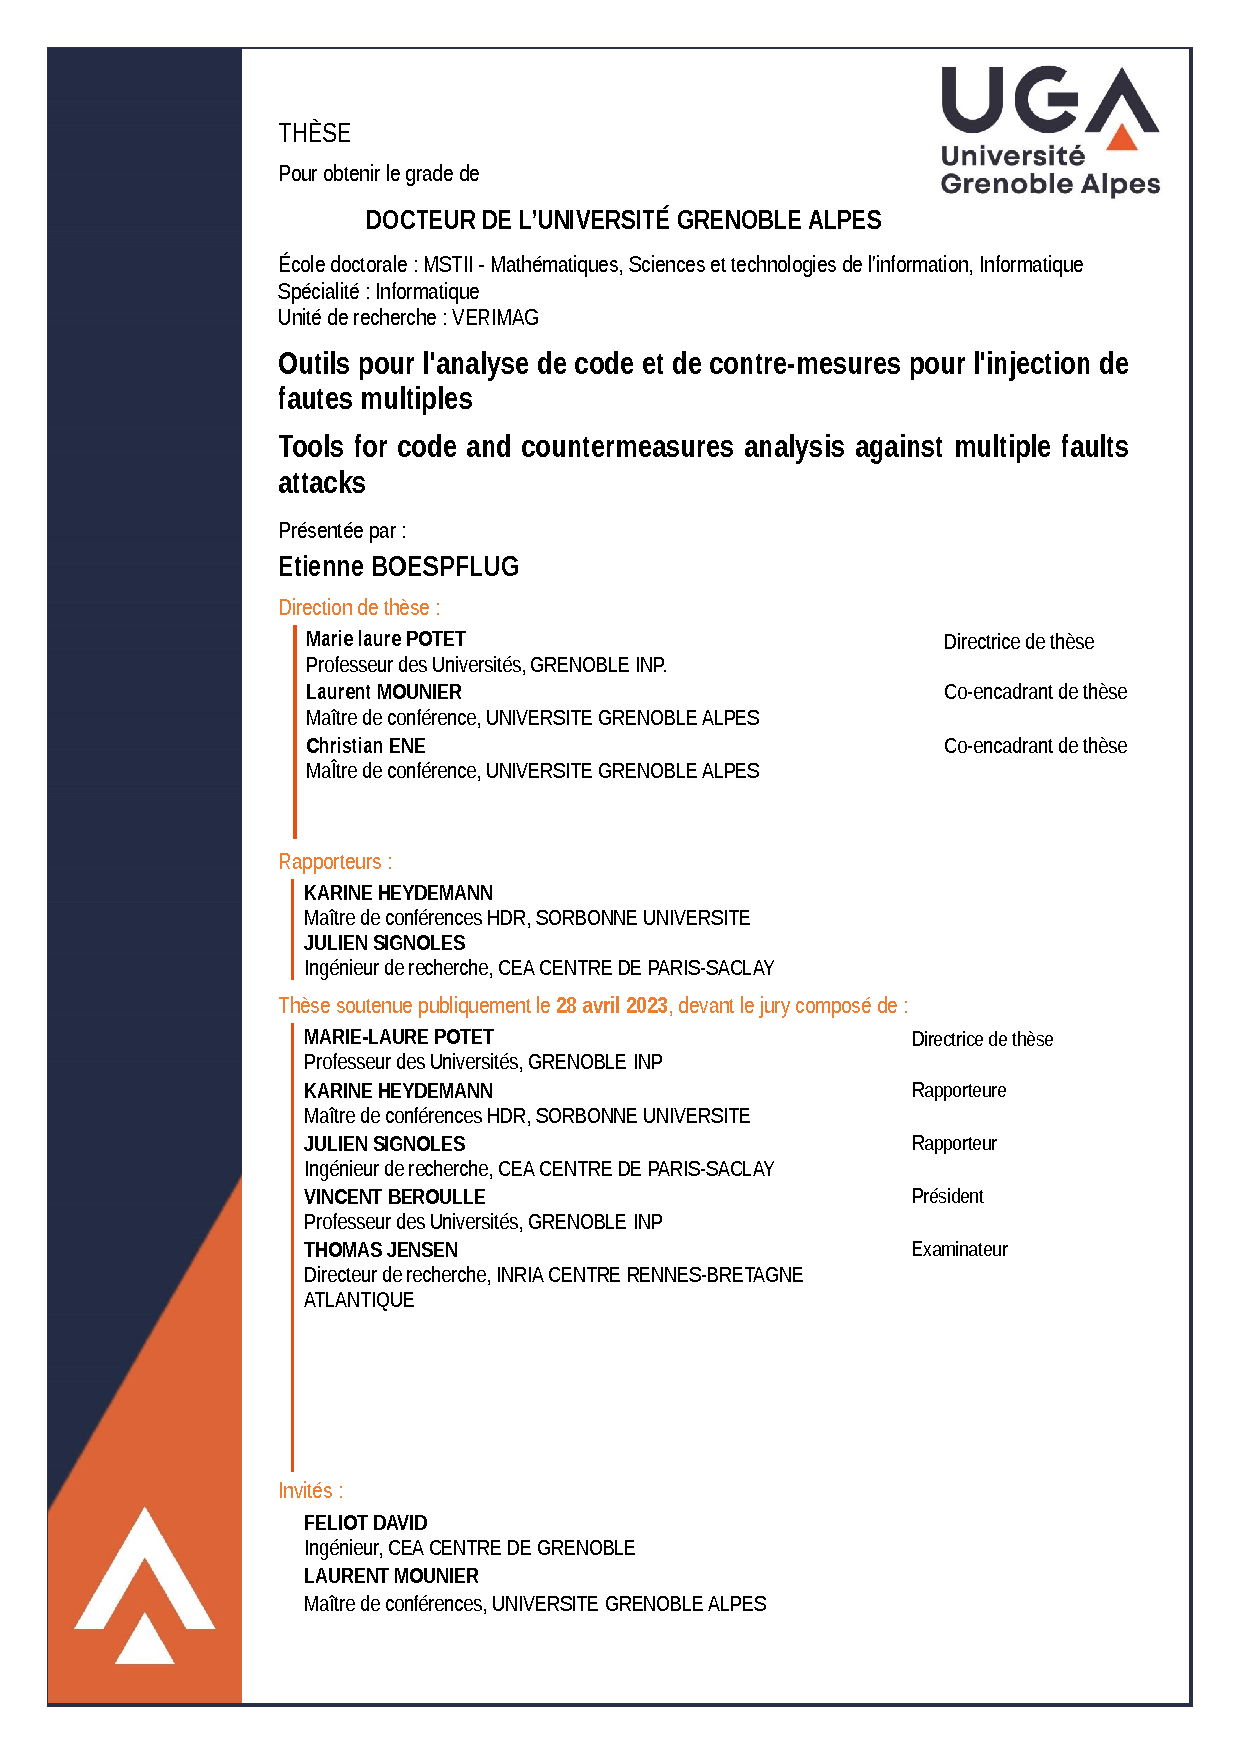
\includepdf[pages=-]{couverture_these.pdf}

\pagenumbering{roman}

\setcounter{page}{0}
\cleardoublepage

\section*{Remerciements}

    C'est la dernière page à rédiger pour ce manuscrit, et s'il ne s'agit probablement pas de la plus difficile à écrire, c'est pour autant loin d'être la plus simple. Je m'excuse par avance pour tous ceux que je vais fatalement oublier.
    
    Tout d'abord, mes sincères remerciements à \textit{Marie-Laure Potet}, ma directrice de thèse, qui m'a accompagné tout au long de ces quatre années de doctorat.
    Elle a su me guider et m'apporter son expérience du monde académique et son goût pour la recherche.
    Un grand merci aussi à mes co-encadrants, \textit{Cristian Ene} et tout particulièrement \textit{Laurent Mounier}, qui m'ont aidé et fait profiter de leur expertise dans les domaines de recherche de cette thèse.
    
    Je tiens aussi à remercier \textit{Karine Heydemann} et \textit{Julien Signoles}, mes rapporteurs, qui ont pris le temps de lire soigneusement toutes les pages de ce manuscrit et de m'en faire un retour pertinent et détaillé.
    Merci tout particulièrement à \textit{Julien} pour m'avoir accompagné depuis le début de la thèse en tant que référent pour le comité de suivi.
    Je remercie aussi les autres membres du jury, \textit{Thomas Jensen}, ainsi que \textit{Vincent Beroulle}, qui m'a fait l'honneur de présider le jury de thèse. 
    Je souhaiterais aussi remercier \textit{David Féliot}, qui m'a fourni des retours et des suggestions concernant l'outil Lazart et avec qui j'ai pu collaborer pour certaines publications. 
    
    Je voudrais aussi exprimer ma gratitude envers les membres permanents du laboratoire VERIMAG. Je n'ai pas eu la chance de tous vous connaître personnellement mais j'ai fait des rencontres enrichissantes et les discussions en salle de repos m'ont souvent été d'une grande aide sur le plan académique, technique et personnel.
    Je voudrais remercier tout particulièrement \textit{Erwann Jahier} et \textit{Patrick Fulconis}, qui m'ont sorti de situations techniques délicates et m'ont apporté de précieux conseils.
    Merci aussi aux différents doctorants et stagiaires que j'ai pu rencontrer au cours de ma thèse. Particulièrement mes collègues de bureau, \textit{Vincent Werner} et \textit{Maxime Lesourd}, pour les soirées bières et les discussions autour d'un café, \textit{Guilhem Lacombe} pour son travail sur Lazart et les projets de recherche qui ont été menés par la suite, \textit{Thomas Vigouroux} pour les moments de rire et son soutien sur la période difficile de la rédaction (le saumon fumé viendra un jour).
    Mes remerciements vont aussi à tous ceux que j'ai pu croiser que de façon occasionnelle, à \textit{Louis Dureuil} et \textit{Maxime Puys} (d'autant plus pour leur travail antérieur sur Lazart qui a été une excellente base pour le développement de l'outil), ainsi qu'à \textit{Soline Ducousso}, \textit{Jean-Baptiste Bréjon } et \textit{Johnathan Salwan} et bien d'autres.
    Je remercie également mes collègues enseignants pour ce qu'ils m'ont apportés durant la période où j'ai enseigné ainsi que les étudiants des différentes promotions de licence et de master qui m'ont fait découvrir cet aspect de la recherche.
    Merci aussi aux chercheurs et intervenants de l'Université de Limoges, où j'ai effectué ma licence et mon master, qui ont su me donner goût à l'informatique, la sécurité et la recherche. Ainsi qu'à mes camarades de promotions, pour les moments de rigolades et de sérieux qu'on a pu passer ensemble.
    Merci à tous ceux du monde académique et industriel que j'ai pu rencontrer au cours de réunions, séminaires, écoles d'été ou colloques, et merci à ceux qui ont réalisé les différents travaux qui m'ont inspiré et sur lesquels je me suis basé pour les recherches présentées dans ce manuscrit.
    
    À ma famille, ma mère \textit{Magali}, mon père \textit{Hervé} et mes deux frères, \textit{Vincent} et \textit{Arnaud}, qui ont été un soutien important pendant les moments difficiles, de doutes et de remise en question. 
    Un remerciement tout particulier à mes amies et amis qui m'ont accompagné et soutenu pendant cette thèse, chacun à sa manière : \textit{Audrey}, \textit{Aurélie}, \textit{Benjamin}, \textit{Clément}, \textit{Coraline}, \textit{Élise}, \textit{Étienne}, \textit{Fabien}, \textit{Florian}, \textit{Hildéric}, \textit{Jean-Baptiste}, \textit{Joris}, \textit{Julia}, \textit{Julie}, \textit{Mallaury}, \textit{Mélisse}, \textit{Morgan}, \textit{Pierre-Olivier}, \textit{Sophie}, les nombreux \textit{Thomas}, \textit{Quentin}, \textit{Victor}, ainsi que tous ceux de chez Origin.
    Enfin, merci à tous ceux que je n'ai pas pu citer ou que j'aurais oublié, ce manuscrit n'aurait pas vu le jour sans les conseils et le soutien qui m'ont été apportés au cours de ces quatre années de thèse. 

% Abstract
\cleardoublepage
\begin{vcenterpage}
    \noindent\rule[2pt]{\textwidth}{0.5pt}
    {\large\textbf{Outils pour l’analyse de code et de contre-mesures pour l'injection de fautes multiples\\}}
    {\large\textbf{Résumé :}}
    
        Les attaquants actifs sont capables d'intervenir sur le comportement du programme pendant son exécution. En particulier, les attaques par injection de fautes, qui ont émergées à l'origine en tant que méthode de test contre les fautes matérielles accidentelles, sont un vecteur d'attaque puissant dans lequel l'attaquant peut injecter des \textit{fautes} pendant l'exécution à l'aide de techniques physiques telles que les faisceaux lasers \cite{Roscian/FDTC13, Colombier/HOST19} ou des glitches de tension \cite{BarEl/IEEE06} ou de fréquence \cite{Agoyan/SCRAA10, Yuce/HSS18}. Plus récemment, des méthodes d'injection de fautes logicielles sont apparues \cite{Park/IIRW14}.
        Cette thèse s'intéresse à l'analyse de programmes dans le contexte des attaques en fautes, et plus particulièrement en fautes multiples, qui implique que l'attaquant est capable d'effectuer des attaques combinant plusieurs fautes. 
        Ces attaques combinées complexifient la tâche des outils d'évaluation automatique de robustesse en raison de l'explosion combinatoire des chemins d'exécution due aux fautes.
        
        Ce manuscrit présente les différentes contributions de cette thèse.
        En premier lieu, l'outil d'analyse de robustesse Lazart a été repris et développé au cours de cette thèse et vise à aider la recherche d'attaques dans un programme dans le contexte de fautes multiples.
        L'évaluation des protections contre ce type d'attaques a aussi été un sujet important de cette thèse et des contributions sont présentées pour aider au placement de contre-mesures logicielles.
        Enfin, les outils de placement utilisés dans la littérature se basent souvent sur une approche essais / erreurs qui n'est pas adaptée au contexte d'attaques multiples et s'intéressent rarement à montrer que les protections sont effectivement utiles. Une méthodologie d'optimisation de programmes protégés a été développée, visant à déterminer quelles portions des protections peuvent être retirées, tout en maintenant le même niveau de sécurité.
    
    {\large\textbf{Mots clés :}}
    Analyse de code, Injection de fautes, Fautes multiples, Contre-mesures logicielles, Évaluation de contre-mesures, Lazart
    \\
    \noindent\rule[2pt]{\textwidth}{0.5pt}
\end{vcenterpage}

\newpage
\begin{vcenterpage}
    \noindent\rule[2pt]{\textwidth}{0.5pt}
    \begin{center}
    {\large\textbf{Tools for code and countermeasures analysis against multiple faults attacks\\}}
    \end{center}
    {\large\textbf{Abstract:}}
    
        Active attackers are able to modify the behavior of the program during its execution. In particular, fault injection attacks, which originally emerged as a method of testing against accidental hardware faults, are a powerful attack vector in which the attacker can inject faults during execution using physical techniques such as laser beams \cite{Roscian/FDTC13, Colombier/HOST19}, or voltage \cite{BarEl/IEEE06} or frequency glitches \cite{Agoyan/SCRAA10, Yuce/HSS18}. More recently, software fault injection methods have been proposed \cite{Park/IIRW14}.
        
        This thesis focuses on analysing programs in the context of fault injection attacks, and more particularly multiple faults, which implies that the attacker is able to combine several faults to complete an attack.
        Combined attacks make more difficult the evaluation of the robustness of programs by tools because of the combinatorial explosion of the execution paths due to faults.
        
        This manuscript presents the different contributions of this thesis.
        First, the robustness analysis tool Lazart has been developped during this thesis, aiming at helping the
        search of attacks on software in a multi-fault contex.
        The evaluation of protections against this type of attacks has also been an important topic of this thesis and contribution are presented to assist the placement of software countermeasures.
        Finally, the placement tools used in the literature are often based on a trial-and-error approach that is not adapted to multiple fault contexts, and they rarely address the verification that these protections are effectively useful in the program. A methodology to optimise the placementof countermeasures has been developed, able to determine which portions of the protections in a program can be removed,  while maintaining the same level of security.
    
    {\large\textbf{Keywords:}}
    Code analysis, Fault injection, Multiple faults, Software countermeasures, Countermeasure evaluation, Lazart
    \\
    \noindent\rule[2pt]{\textwidth}{0.5pt}
\end{vcenterpage}

\newpage

% Tables of Contents
\dominitoc
\setcounter{tocdepth}{1}
\tableofcontents

\etocsettocstyle{}{} % from now on only local tocs

\listoffigures

\listoftables

\lstlistoflistings

\printglossaries

% Content
\mainmatter

%\part{Analyse de robustesse et injection de fautes}
\chapter{Contexte}
\label{chpt:contexte}
    
    \section*{Table des Matières}
    \localtableofcontents
    
    \section{Garantir la sécurité d'un programme ou d'un système}
    
        La sûreté et la sécurité des programmes et des systèmes sont des enjeux majeurs de nos jours. 
        
        La \textit{sûreté} se réfère à l'ensemble des risques dont la cause est accidentelle. La \textit{sécurité} concerne quant à elle les actes de malveillance.
        Si on prend pour analogie un aéroport, la panne d'un avion correspond à un risque de l'ordre de la sûreté tandis qu'un attentat relève de la sécurité.
        Une \textit{attaque} correspond à une tentative d'un adversaire (appelé \textit{attaquant}) d'obtenir un avantage sur un système. 
        Cet avantage peut se traduire par une élévation de privilèges \cite{Timmers/FDTC16} ou l'accès à des données sensibles \cite{Biham/AICC97} par exemple, mais dans un cadre général il peut s'agir de tout comportement qui n'a pas été prévu pour le système. 
        Par \textit{système} nous entendrons de manière générique un appareil informatique, un programme, un réseau de sous-systèmes et plus généralement, toute entité traitant de l'information répondant à des besoins de sûreté et susceptible d'être attaquée.
        
        Des ordinateurs aux téléphones modernes, en passant par les appareils connectés ou encore les cartes à puces, le nombre de systèmes et de technologies disponibles continue de croître \cite{HardwareEmbeddedSystems}. La surface d'attaque globale ne cesse donc de grandir, et la diversité des attaques qui doivent être prises en compte lors de la mise en place d'un système rend le processus de développement plus complexe. 
        
        Pour parer à ces menaces, des protections sont mises en oeuvre de manière à détecter ou bloquer les attaques. Ces protections peuvent prendre la forme de transformations du programme source, par exemple en modifiant l'algorithme \cite{Aumuller/CHES02} ou en rajoutant du code visant à détecter et/ou empêcher les attaques  \cite{Reis/ISCCO05, lalande}. Les protections peuvent aussi être appliquées au niveau de la plateforme, comme par exemple la randomisation de l'espace mémoire par le système d'exploitation de manière à rendre l'exploitation des attaques plus difficiles \cite{shacham2004effectiveness}. Ou encore, au niveau matériel, en ajoutant des protections physiques dans le composant de manière à limiter la lecture des données stockées \cite{Boneh/EUROCRYPT97}.
        
        De nouvelles attaques sont découvertes et mènent à la recherche de nouvelles protections qui sont par la suite attaquées à leur tour. Ainsi, les attaquants se diversifient et un système doit faire face à des menaces variées. 
        
        \begin{probl}
        \label{prob:help-dev}
            Comment faciliter le processus de développement d'un logiciel afin d'aider le développeur dans le choix et la mise en place des protections ?
        \end{probl}
        
        Plus encore, une nouvelle attaque peut être découverte après l'analyse de la sécurité d'un programme et ainsi mettre en lumière de nouvelles vulnérabilités. Les processus d'évaluation et de protection d'un système doivent donc être réexaminés à intervalles réguliers de manière à prendre en compte les nouvelles menaces. 
        
        Bien entendu, le niveau de sécurité dépend grandement du contexte d'utilisation d'un système. La confidentialité des communications d'un satellite militaire doit répondre à un niveau de sécurité plus élevé que celle d'une boite au lettre d'un particulier par exemple. A l'inverse, une serrure pour une résidence est une protection contre les tentatives d'intrusion dont la nécessité est discutable pour un satellite. Il est nécessaire d'évaluer le risque d'une attaque en fonction du niveau de sécurité qu'on souhaite atteindre et en fonction du système à protéger. La balance bénéfice/coût de l'attaquant est à prendre en compte par le défenseur pour évaluer les menaces du système.
        
        Pour permettre de certifier la sûreté et la sécurité d'un système, des méthodologies ont été développées. La certification \gls{cc} \cite{CommonCriteria17} est un processus de certification standardisé par la norme \gls{iso} 15408 permettant à des organismes spécialisés de garantir un certain niveau de sécurité sur un système. Les \gls{cc} proposent un ensemble de procédures permettant d'obtenir un niveau d'assurance sur la sécurité du système en question. Ainsi, il est possible de viser un type de certification en fonction du niveau de sécurité voulu. La figure \ref{tbl:common-criterias-levels} présente les différents niveaux d'assurance des \gls{cc}, chacun définissant un seuil de mise en place de moyens humains, d'expertise et de technologie par le fournisseur du produit et l'organisme de certification et des critères en fonction des problèmes découverts pour l'obtention ou non du certificat. 
        
        \begin{table}
        {\small
            \begin{center}
\begin{tabular}{cc}
\hline
EAL  & Description                                     \\ \hline
EAL1 & Testé fonctionnellement                         \\
EAL2 & Testé structurellement                          \\
EAL3 & Méthodiquement testé et vérifié                 \\
EAL4 & Méthodiquement conçu, testé et revu             \\
EAL5 & Semi-formellement conçu et testé                \\
EAL6 & Conception semi-formellement vérifiée et testée \\
EAL7 & Conception formellement vérifiée et testée      \\ \hline
\end{tabular}
            \end{center}
            }
                \caption{Les différents niveaux de certification des Critères Communs \cite{Dureuil/Phd16}}
                \label{tbl:common-criterias-levels}
\end{table}

        De la même manière, les audits de sécurité sont effectués pour les systèmes d'information et mettent en place des scénarios d'attaque variés de manière à s'assurer de la sécurité du système. Des tests d'intrusion (les \textit{pentests}) sont mis en oeuvre afin de simuler différents types d'attaquant et de vérifier la réaction du système.  
        Différents modèles d'attaquant sont considérés, en allant du test en boite noire où le système est inconnu de l'attaquant et qui se place à l'extérieur de celui-ci, au test en boite blanche où l'attaquant est modélisé comme connaissant les détails internes du système ou comme ayant un accès privilégié dans le système. 
        
        \begin{probl}
        \label{prob:help-auditor}
            Comment faciliter le processus d'évaluation par l'expert d'un programme et de ses protections à l'aide de méthodologies et d'outils ?
        \end{probl}
        
        La sécurité a un coût, à la fois en termes de moyens humains et d'expertise mais également parce que les protections peuvent complexifier le système, ou altérer les performances (rapidité d'exécution inférieure, taille du code plus grande...). De plus, d'autres problématiques industrielles comme des délais de production ou des limitation matérielles viennent se combiner à celle de la sécurité. 
        Par exemple, les processeurs modernes utilisent une optimisation appelée l'exécution spéculative qui vise à exécuter une branche d'un programme avant que la condition de branchement soit évaluée. Si la mauvaise branche a été choisie, la pipeline est déroulée pour revenir à son état précédent pour exécuter la bonne branche. Cette technique permet de fournir une performance accrue pour le processeur. Néanmoins, l'attaque Spectre, découverte en 2019 \cite{Kocher/SP2019}, a démontré qu'il était possible d'exploiter les effets de bord de cette optimisation de manière à retrouver des informations secrètes qui ne sont normalement pas accessibles. Un compromis est souvent nécessaire entre les différentes problématiques (sûreté, sécurité, performance, accessibilité etc.) liées au développement d'un système.
        
        Chaque couche ou noeud d'un système pouvant être menacé, une attaque peut être composée de plusieurs attaques visant des parties différentes du système. Par exemple, l'attaque \textit{Rowhammer} \cite{Kim/ACM14, Park/IIRW14}, permet à un attaquant de tirer profit d'effets de bord dans le fonctionnement des cellules mémoires \gls{dram} pour augmenter le niveau de privilèges sur une machine sans nécessité d'accès physique. 
        Ce fut aussi le cas lors du challenge \textit{Wookey} \cite{SSTIC20} où un chemin d'attaque hybride a été détecté dans lequel la protection contre le dépassement de tampon implémentée dans l'interface de carte à puce (\gls{iso} 7816) est contournée par une attaque physique. La combinaison des deux attaques permet d'obtenir une élévation de privilège. 
        
        \begin{probl}
        \label{prob:high-order-analysis}
            Comment évaluer un programme et ses protections dans un contexte d'attaques multiples ?
        \end{probl}
        
        Cette thèse s'inscrit dans ce contexte et vise à proposer des solutions pour la protection et l'évaluation d'un programme et de ses protections. Ce chapitre présente des problématiques générales liées à l'analyse de programmes et de protections ainsi que les contributions apportées dans cette thèse. 

        \subsection*{L'exemple verify\_pin}
            
            Le programme présenté dans le listing \ref{lst:verifyPIN-BU} est une version naïve d'un processus de vérification de code \gls{pin} en langage C. Ce programme servira d'exemple pour présenter les enjeux et les problématiques de la protection et l'analyse de programmes. 
            
\lstset{caption={Programme verify\_pin \og naif \fg{} },label=lst:verifyPIN-BU}
\begin{lstlisting}
// PIN secret.
static uint8_t card_pin[5] = {'0', '1', '2', '3', '\0'}; 
static int try_counter = 3;

bool compare(uint8_t* a1, uint8_t* a2)
{
    int i = 0;
    while(*a1 != '\0') {
        if(*a1 != *a2)
            return false;

        ++a1; ++a2;
    }

    return true;
}

bool verify_pin(uint8_t* user_pin) { 
    if(try_counter > 0) {    
        if(compare(card_pin, user_pin)) {
            try_counter = 3;
            return true;
        } else {
            try_counter--;
            return false;
        }
    }

    return false;
}
\end{lstlisting}

        La figure \ref{fig:verifyPIN-spec} est un schéma d'utilisation fonctionnel de ce programme. L'authentification nécessite que le compteur d'essais soit strictement positif et que le \gls{pin} d'entrée soit identique à celui de la carte.
        Le programme \texttt{verify\_pin} est décomposé en deux: la fonction \texttt{verify\_pin} prend en argument le \gls{pin} utilisateur et appelle la fonction \texttt{compare} qui se charge de comparer les deux chaînes correspondant aux \gls{pin}s.        
        
        \begin{figure}[!ht]\centering
            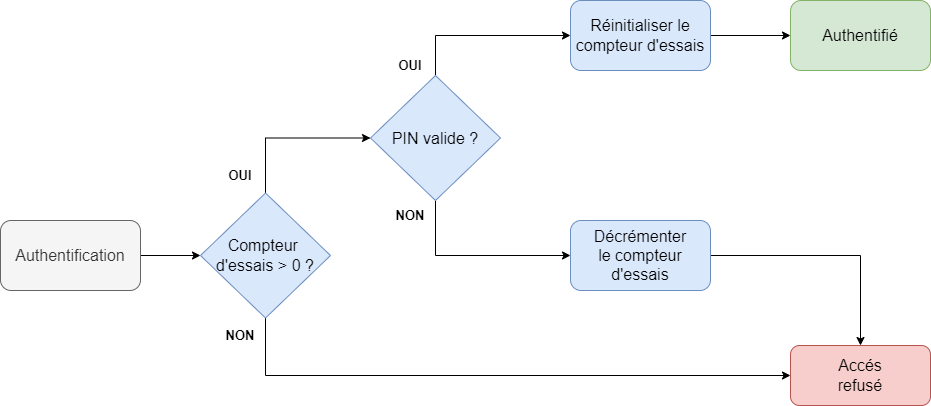
\includegraphics[scale=0.4]{ch1-context/img/verifyPINSpec.png}
            \caption{Schéma fonctionnel du programme \textit{verify\_pin}}  \label{fig:verifyPIN-spec}
        \end{figure}
        
        Dans la fonction principale, un compteur d'essai est vérifié de manière à limiter le nombre d'erreurs d'entrées successives autorisées. Le compteur est décrémenté en cas d'échec et remis à la valeur 3 lorsque l'authentification est un succès. Le \gls{pin} secret \texttt{card\_pin} est modélisé par un tableau statique pour cet exemple (ce qui n'est pas le cas dans la réalité).        
        
        La fonction \texttt{compare} effectue une comparaison de deux chaînes en bouclant sur chaque caractère jusqu'à atteindre un caractère terminant par le caractère nul `\textbackslash0'. Si deux caractères sont différents, la boucle se termine prématurément en retournant \textit{faux}. Cela correspond à ce qui est fait par des fonctions C standards telles que \texttt{strcmp}.
        Les deux fonctions retournent des valeurs booléennes \textit{vrai} et \textit{faux} respectivement représentées par les entiers $1$ et $0$.
        
        Ce programme illustre une problématique d'authentification qui est présente dans un grand nombre d'objets sécurisés, par exemple les cartes \gls{sim} des téléphones ou les cartes à puces.     
        
    \section{Modèles d'attaquant et objectif d'attaque}
    \label{sec:model-attack}
    
        Lorsqu'on s'intéresse à la sécurité d'un programme, il est nécessaire de définir l'adversaire contre lequel on souhaite se protéger, ce qui se traduit par le \textit{modèle d'attaquant}.
        
        On aimerait dans l'idéal pouvoir rester le plus général possible, mais en pratique les outils et méthodes d'analyse restreignent le contexte dans lequel le programme est étudié. Cela est fait d'une part, pour maintenir des temps de calcul réalistes et d'autre part, parce qu'il n'y a pas de limite théorique à la puissance d'un attaquant, qui va dépendre du contexte et des moyens mis en oeuvre. Si un programme est sécurisé face à un modèle d'attaquant précis, rien n'empêche qu'un autre type d'attaque soit découvert par la suite et remette en question la sécurité du programme. 
        
        \begin{probl}
        \label{prob:attack-model}
            Comment définir et modéliser un attaquant dans le contexte d'une analyse de sécurité ?
        \end{probl}
        
        Le \textit{modèle d'attaquant} peut être vu comme un ensemble contenant : l'objectif d'attaque et le pouvoir de l'attaquant, comme présenté dans la figure \ref{fig:attacker-model}.
        
        \begin{figure}[!ht]\centering
            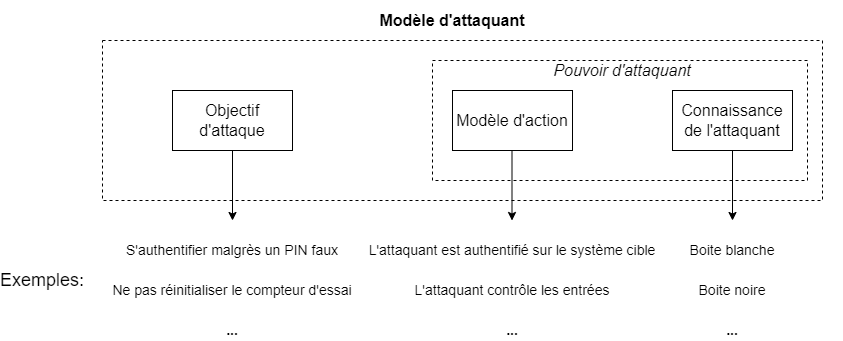
\includegraphics[width=\textwidth]{ch1-context/img/attack-model.png}
            \caption{Modèle d'attaquant}  \label{fig:attacker-model}
        \end{figure}
        
        On appelle \textit{objectif d'attaque} la propriété de sécurité visée par un adversaire. Pour l'exemple \textit{verify\_pin}, un objectif d'attaque naturel consiste à s'authentifier sans connaître le code de la carte. Un second objectif peut être de ne pas décrémenter le compteur d'essais lors d'un échec d'authentification. 
        
        On appelle \textit{modèle d'action}, l'ensemble des actions qu'un attaquant est capable d'effectuer sur le système cible. La \textit{surface d'attaque} correspond à l'ensemble des points du système sur lesquels l'attaquant effectue ses actions et est donc directement liée au modèle d'action considéré.
        
        Une \textit{vulnérabilité} est une faiblesse, dans une implémentation ou un système, pouvant être exploitée par un adversaire. Une vulnérabilité peut être un système mal configuré, non mis à jour, une erreur dans un logiciel, l'usage d'algorithme cryptographique non sûr ou même d'ordre organisationnel comme la présence d'un adversaire au sein du personnel de l'entreprise par exemple. Une vulnérabilité est intrinsèquement liée à un modèle d'attaquant, par exemple un programme peut être vulnérable aux dépassements de tampon ou à un défaut d'alimentation.
        
        On parle d'\textit{exploitation} pour désigner un programme ou une méthode permettant d'exploiter une vulnérabilité dans un système (en obtenant une élévation de privilège par exemple). La présence d'une vulnérabilité n'implique pas forcément qu'une exploitation soit possible dans l'immédiat. Par exemple, l'attaque \textit{Rowhammer} présentée précédemment a été d'abord théorisée \cite{Kim/ACM14} puis exploitée plus tard ~\cite{Seaborn/BH15,Gruss/DIMVA16}. Une vulnérabilité peut potentiellement être exploitée bien après sa découverte. Dans l'exemple \textit{verify\_pin}, une vulnérabilité sur la ré-initialisation du compteur de boucle en cas d'échec pourrait être exploitée pour obtenir un accès à la carte à l'aide d'une attaque par force brute.
        
        Enfin, le modèle d'attaquant inclus aussi la connaissance qu'un adversaire a sur sa cible, la \textit{connaissance de l'attaquant}. C'est ce que représente la diversité des tests en certification par exemple avec des attaquants agissant sur un système en boite noire ou en ayant un accès et une connaissance plus ou moins étendue sur le système. La \gls{jil} \cite{JIL} fait la distinction entre différents niveaux d'expertise reflétant la capacité d'un attaquant à utiliser des outils d'audit ou à créer de nouvelles attaques. Cette modélisation de la connaissance de l'adversaire sur le système permet aussi d'évaluer le risque que présente une vulnérabilité sur le système lors des processus d'audit. Un attaquant ayant un accès et des connaissances privilégiés sur le système est plus dangereux mais moins probable.
        
        En allant d'un attaquant ne contrôlant que les entrées du programme à un adversaire infiltré en tant d'administrateur sur la machine cible, le modèle d'attaquant peut radicalement varier en fonction du cadre d'usage du programme et des techniques d'attaques connues. Les exploitations peuvent mettre en oeuvre plusieurs types d'attaques, comme dans l'exemple \textit{Wookey} évoqué précédemment, et demande donc de prendre en compte des objectifs d'attaque variés.
        
        Dans le cadre de l'analyse logicielle, les outils et les techniques d'analyses doivent faire face à la diversité des modèles d'attaquants, bien que actuellement ils soient souvent spécifiques à des classes d'attaques particulières.
        
        \begin{probl}
            \label{prob:evolving-models}
            Comment faciliter l'analyse et la protection de programme pour des modèles d'attaquants qui évoluent et se complexifient ? 
        \end{probl}
        
    \section{Analyse de programmes}
    \label{sec:analysis}
        
        \begin{sloppypar}
        Le problème de l'arrêt énoncé par Alan Turing \cite{Turing/37} a montré qu'il n'existe pas de méthode d'analyse automatique permettant de savoir si un programme termine ou non. Lorsqu'on s'intéresse à la vérification de propriétés non triviales sur un programme, on se confronte au problème de l'indécidabilité \cite{Bradley/VMCAI06}. Toutefois, il existe des méthodes pour étudier le comportement d'un programme malgré cette limitation.
        \end{sloppypar}
        
        La fonction \texttt{foo} présentée dans le listing \ref{lst:foo-program} prend en entrée les variables $a$, $b$ et $c$ et calcule $a*b*c$. Même dans un cas simple comme celui-ci, il n'est pas trivial de s'assurer que la fonction se comporte toujours correctement.

\begin{lstlisting}[caption={Fonction foo}, label=lst:foo-program]
int foo(int a, int b, int c) {
    int total = 0;
    for(int i = 0; i < c; ++i)
        total += a * b;
    return total;
}
\end{lstlisting}        

        La fonction \textit{foo} possède un nombre fini d'\textit{exécutions} différentes possibles. Les entrées sont constituées seulement des trois variables  $a$, $b$ et $c$, mais il reste difficile de tester par force brute toutes les combinaisons d'entrées ($2^{96}$ possibilités dans le cas d'entiers codés sur 32 bits).
        Plus encore, certains programmes peuvent potentiellement avoir un nombre d'exécutions infinies. Le système peut attendre des entrées utilisateurs ou un évènement réseau sans limite finie, ce qui rend impossible l'exploration exhaustive des exécutions dans le cas de boucles ou de cycles infinis.
        
        Même si on pouvait effectuer une analyse exhaustive des exécutions, la question de la modélisation du système est aussi une problématique majeure. En effet, si on veut par exemple s'intéresser aux effets d'un dépassement de capacité du type entier dans la fonction \texttt{foo}, il faut prendre en compte l'encodage utilisé et les spécificités des architectures cibles. 
        Pour pallier ce problème, il est possible d'effectuer ces tests sur une véritable machine ce qui apporte des garanties concernant la précision de l'analyse mais nécessite la mise en place d'un banc de test physique et rend l'analyse spécifique au système de test choisi \cite{Faurax/Phd09}.
        
        De nombreuses techniques d'analyses ont été développées pour la vérification de programmes, que ce soit dans le domaine de la sécurité ou de la sûreté. Les méthodes d'analyses peuvent être classées en quatre catégories, présentées dans la figure \ref{fig:analysis-methods}, en fonction de leur approximation de l'ensemble des exécutions du programme étudié.
    
        \begin{figure}[!ht]
            \centering
            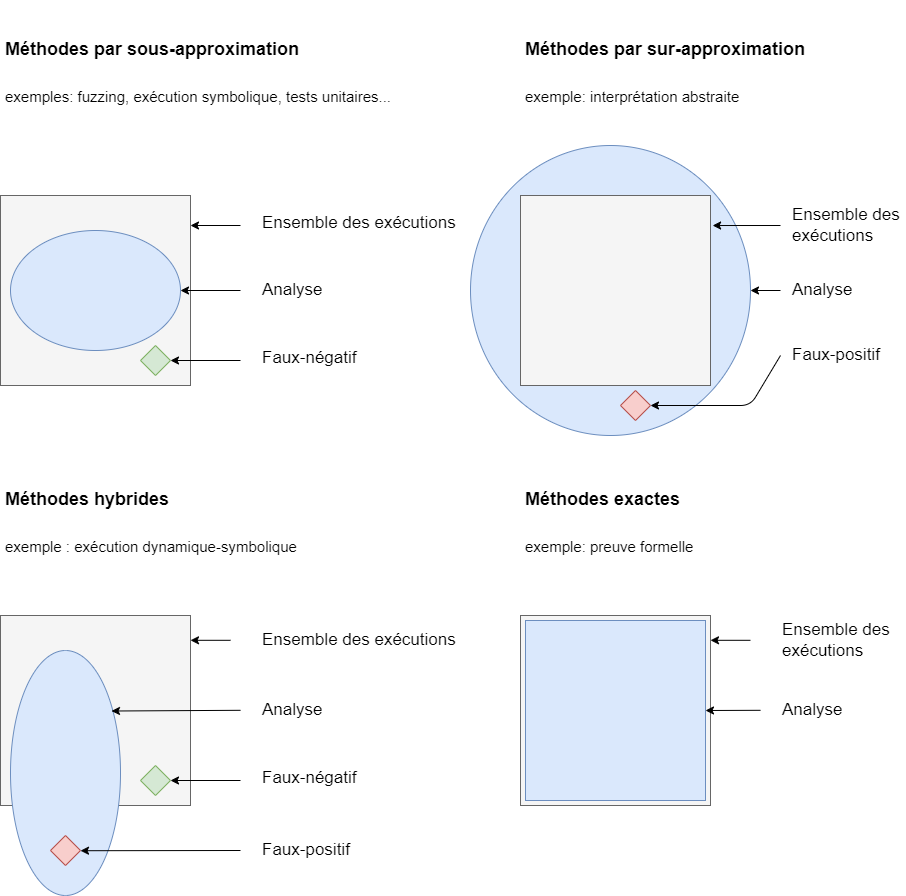
\includegraphics[scale=0.56]{ch1-context/img/analysis.drawio.fr.png}
            \caption{Méthodes d'analyses statiques} \label{fig:analysis-methods}           
        \end{figure}           
        
        Les \textit{méthodes par sous-approximations} étudient un sous-ensemble des exécutions possibles d'un programme. L'exemple naturel est le test. Les tests unitaires sont très utilisés en développement logiciel et consistent à tester indépendamment des fonctions et des modules d'un programme en se concentrant souvent sur les cas qui sont à priori susceptibles d'entraîner des erreurs (telles que les bornes du type des entrées ou des valeurs interdites par la spécification par exemple). 
        Le fuzzing \cite{Manes/TSE19} est une autre méthode de génération de test où les entrées sont choisies aléatoirement (ou semi-aléatoirement à l'aide d'heuristiques).
        L'exécution symbolique \cite{King/ACM76} (qui sera détaillé dans la section \ref{sec:se}) est aussi une méthode de génération de tests qui effectue une sous-approximation de l'ensemble des exécutions. 
        
        \begin{sloppypar}  
        A l'inverse, les \textit{méthodes par sur-approximation} produisent des faux-positifs puisqu'elles s'intéressent à un sur-ensemble des exécutions possibles. L'interprétation abstraite \cite{cousot1977abstract, Cousot/CSL14} est un exemple de méthode par sur-approximation. Le plugin \gls{eva} de Frama-C \cite{FramaC-EVA} utilise l'interprétation abstraite au niveau C. C'est aussi le cas des analyses faites par les compilateurs pour savoir si certaines transformations ou optimisations sur un programme peuvent être effectuées sans changer la sémantique d'un programme. 
        \end{sloppypar}   
      
        Les \textit{méthodes exactes} permettent de caractériser les exécutions d'un programme de manière exacte. La preuve formelle par exemple, consiste à prouver formellement qu'un programme est correct, à l'aide de théories mathématiques. Cela étant, ces techniques ne sont pas entièrement automatiques puisque le problème est indécidable en général. Les assistants de preuves tels que Coq \cite{Coq}, Isabelle \cite{Nipokow/SSBM02} ou encore le plugin WP de Frama-C \cite{FramaC-wp} assistent l'utilisateur qui peut être amené à effectuer une partie du travail d'analyse.
        
        Certaines méthodes présentent à la fois des faux-positifs et des faux-négatifs. L'exécution concolique \cite{Baldoni/CSUR18} est un exemple de \textit{méthode hybride}. Là encore, de nombreux outils existent comme DART \cite{Godefroid/PLDI05}, KLEE \cite{Cadar/OSDI08} ou encore Angr \cite{Shoshitaishvili/SSP16} pour n'en citer que quelques uns. Plus généralement, les méthodes combinant différentes techniques d'analyse tendent à se classer parmi les méthodes hybrides.
        Le typage dans certains langages de programmation peut aussi entrer dans cette catégorie.
        
        Cette classification n'est pas stricte et certaines techniques se rangent différemment en fonction du contexte. Le model-checking par exemple considère le programme comme un automate à état finis et permet de vérifier des propriétés sur ce modèle. En fonction de la manière dont est  défini le modèle, l'analyse pourra appartenir à différentes classes. 
        
        Ces méthodes d'analyse disposent chacune d'avantages et d'inconvénients, que ce soit en termes de précisions, de complétude ou de temps d'exécution. Ces caractéristiques dépendent aussi du niveau de représentation auquel l'analyse se situe. Les processus d'évaluation de programmes dans le cadre de la sécurité incluent le plus souvent plusieurs méthodes.
        
    \section{Protéger un programme}
    
        De manière à protéger un système contre des attaquants, des protections sont mises en oeuvre. Ces protections, qu'on appellera aussi \textit{contre-mesures}, visent à détecter ou prévenir les attaques. Celles-ci peuvent être mises en place à différents niveaux d'un système: sur le code source, sur le code machine, au niveau de la plateforme (machine virtuelle, système d'exploitation) ou encore au niveau physique. Dans le cas de protections ajoutées au niveau du code source d'un programme, on parle de protections logicielles. 
    
        Le ver de Morris \cite{morirs-worm}, considéré comme le premier \og ver \fg{} informatique, exploitait une vulnérabilité dans l'utilitaire \textit{finger} à l'aide d'un dépassement de tampon. Les attaques par dépassement de tampon constituent une classe d'attaques communément étudiée. Il s'agit de dépasser l'espace mémoire prévu (pour une chaîne de caractères ou un tableau par exemple) de manière à accéder à des segments de mémoire non prévus initialement. Cela peut par exemple permettre d'écraser l'adresse de retour de manière à rediriger le flot de contrôle vers un code malicieux, appelé \textit{shellcode}.
        
        Le programme \texttt{verify\_pin} présenté précédemment souffre d'une vulnérabilité de ce type, notamment à cause de l'utilisation d'un caractère nul pour la fin de chaîne. Le listing \ref{lst:verifyPIN-fixedloop} présente une variante de la fonction \texttt{compare} dans laquelle la taille est passée en paramètre ce qui constitue une première protection contre les attaques par dépassement de tampon. Les fonctions C \texttt{strcmp} et \texttt{memcmp} ont elles aussi vu naître leurs homologues \texttt{strcmp\_s} et \texttt{memcmp\_s}, prenant en paramètre la taille des chaînes à comparer pour s'assurer que la taille des tableaux n'est pas dépassée (si tant est que la bonne taille est passée en argument).
      
\lstset{caption={verify\_pin avec la taille passée en paramètre},label=lst:verifyPIN-fixedloop}
\begin{lstlisting}  
bool compare(uint8_t* a1, uint8_t* a2, size_t size)
{
    for(size_t i = 0; i < size; i++) {
        if(a1[i] != a2[i]) {
            return false;
        }
    }
    
    return true;
}
\end{lstlisting}  

        Les canaris constituent une autre solution de protection logicielle contre les attaques par dépassement de tampon. Il s'agit de valeurs particulières d'octets qui sont placées entre les tableaux de données (ou le plus souvent entre les parties sensibles, à savoir les valeurs de retour sur la pile). Il est alors possible de vérifier l'intégrité du canari pour détecter certains dépassements de mémoire et prendre les mesures nécessaires (invalidation de la donnée corrompue, arrêt du programme, signalement...). Des variantes existent mais cette méthode, qui est implémentée dans tous les compilateurs actuels, implique une surcharge de la mémoire pour les canaris et des mécanismes de vérification à l'exécution. 
        
        Des techniques comme l'utilisation d'une pile non exécutable visent à empêcher l'exécution d'un shellcode. Néanmoins, l'attaquant peut se servir de \textit{gadget}, c'est-à-dire des portions du programme cible (ou d'une bibliothèque) de tailles généralement assez courtes. Ces portions étant déjà dans la section instruction de la mémoire, il sera possible de les exécuter.
        L'attaquant va alors écraser les adresses de retour de manière à exécuter plusieurs gadgets à la suite et obtenir le comportement souhaité, ce qu'on appelle \gls{rop} \cite{Roemer/TISSEC12}.
        
        L'\gls{aslr}, effectuée au niveau de la plateforme, repose sur la randomisation de l'espace mémoire de manière à rendre plus difficile pour un attaquant de trouver les canaris ou des gadgets par exemple. Dans le même registre, les système d'exploitation peuvent mettre en place un réordonancement aléatoire des adresses mémoires manipulées.
        
        Ces contre-mesures visent à endiguer ou à limiter l'impact des attaques par débordement de tampon. Celles-ci peuvent prendre la forme de transformations du programme source (en ajoutant un argument de taille comme dans l'exemple précédent de \textit{compare}), être appliquées par un outil automatique (par exemple au moment de la compilation comme l'ajout de canaris), être des protections assurées par l'environnement (comme l'\gls{aslr} qui est effectuée par le système d'exploitation, la mise en place de machines virtuelles ou de système de détection d'intrusion (IDS)) ou encore être mises en place au niveau physique (en chiffrant la mémoire de la machine par exemple).
        
        Un autre exemple de protection concerne les attaques par canaux auxiliaires. Celles-ci visent à récupérer des informations à partir de données physiques telles que la consommation d'un composant ou le temps d'exécution. Pour la fonction \texttt{compare} précédente, un attaquant pourrait mesurer le temps d'exécution de la boucle de manière à savoir quel chiffre du code \gls{pin} était invalide et ainsi simplifier la recherche du secret \footnote{Un \gls{pin} à 4 chiffre comporte $10^4$ combinaisons, si un attaquant peut savoir quel chiffre est incorrect il devient alors capable de casser le \gls{pin} en $10 * 4$ essais au maximum.}.
        
        On peut se protéger de ce type d'attaque en transformant la boucle de la manière à la rendre en \textit{temps constant}, comme présenté dans le listing \ref{lst:verifyPIN-sidechannel} où la boucle n'est pas terminée prématurément en cas d'échec et où la condition est remplacée par une opération bit à bit. Un large éventail de protections logicielles et matérielles a été développé pour ce type d'attaque également \cite{Wittman/RSA08, Veryrat/TACIS12}.
        
\lstset{caption={verify\_pin en temps constant},label=lst:verifyPIN-sidechannel}
\begin{lstlisting}  
bool compare(uint8_t* a1, uint8_t* a2, uint8_t size)
{
    bool result = true;
    for(size_t i = 0; i < size; i++) 
        result |= a[i] ^ b[i];

    return result;
}
\end{lstlisting} 

        \begin{probl}
            \label{prob:cm-selection}
            Étant donné un modèle d'attaquant et un programme à protéger, comment aider au choix des contre-mesures ?
        \end{probl}
        
        La recherche de la meilleure contre-mesure implique la nécessité d'être capable d'analyser la robustesse d'un programme protégé ou de comparer différents programmes protégés. Des méthodes et des outils doivent donc être mis en place pour aider à l'analyse des contre-mesures.

    \section{Analyser les contre-mesures}
    \label{sec:ctx.cm}

        L'analyse de contre-mesures a plusieurs objectifs: en amont du processus de développement, l'aide au développeur pour la sélection et la mise en place des protections, et en aval, l'aide à l'auditeur pour la recherche de vulnérabilités et la comparaison de différents moyens de protection. Cette analyse se fait en fonction d'un modèle d'attaquant défini.

        En plus de renforcer la sécurité, d'autres paramètres concernant les contre-mesures sont à étudier. Il peut s'agir de métriques de performances (vitesse d'exécution, taille du programme, consommation en mémoire / courant), de contraintes matérielles ou encore de préoccupations telles que la facilité de déploiement ou d'automatisation (par exemple si la contre-mesure nécessite des primitives cryptographiques qui ne sont pas disponibles sur toutes les plateformes).
        Le plus souvent il est nécessaire de faire un compromis entre ces différents paramètres. Le problème de la performance est d'autant plus présent dans le monde de l'Internet des objets (\gls{iot}) ou des composants sécurisés tels que les cartes à puces. En effet, la puissance du matériel est limité mais ces appareils contiennent potentiellement des données sensibles comme des clefs de chiffrement ou des certificats par exemple.

        L'analyse des contre-mesures d'un programme peut être faite de différentes manières. L'utilisation d'ensembles de cas de tests, appelés \textit{benchmark}, permet aux concepteurs de contre-mesures de comparer leurs résultats à ceux obtenus par des contre-mesures existantes. L'évaluation de la protection dépend alors de la représentativité du benchmark choisi, ce qui peut être difficile à estimer. 
        La comparaison des versions protégées d'un programme peut alors être réalisée en comparant des métriques d'analyse. Il peut s'agir, entre autres, du nombre d'attaques trouvées ou du nombre d'attaques pondéré par la taille du programme. 
        La \textit{vérification formelle} peut aussi être utilisée pour effectuer une preuve que le programme protégé n'est pas vulnérable en cas d'attaque \cite{Rauzy/CE14, Moro/JCE14}.
        Les contre-mesures sont généralement pensées pour protéger le programme contre un modèle précis et la question de savoir si toutes les protections sont effectivement utiles est plus rarement considérée. 
        De plus, les contre-mesures étant parfois placée automatiquement, par la chaîne de compilation par exemple, la nécessité d'outils capables d'évaluer automatiquement la pertinence des protections est d'autant plus importante.
        
        \begin{probl}
            \label{prob:cm-effective}
            Comment s'assurer que les protections ajoutées à un programme sont effectivement utiles dans le modèle d'attaquant considéré ? Peut-on en enlever ?
        \end{probl}

        \begin{sloppypar}
        Les modèles d'attaquants puissants complexifient d'autant plus l'analyse que le nombre d'attaques et de chemins d'exécution à étudier peuvent devenir importants. Les attaques composées de plusieurs attaques, appelées \textit{attaques multiples}, comme c'est le cas dans l'exemple Wookey \cite{inter_cesti} cité précédemment, permettent d'attaquer les contre-mesures elles-mêmes: la première attaque neutralise la contre-mesure et une seconde exploite cette absence de protection.
        \end{sloppypar}
        
        \begin{probl}
            \label{prob:cm-multi-fault}
            Comment faciliter la mise en place de contre-mesures dans un contexte d'attaques multiples ?
        \end{probl}
            
    \section{Contributions et organisation du manuscrit}
    
        \subsection{Contributions} 
            
            Cette thèse s'intéresse aux attaques multiples dans lesquelles l'attaquant est actif, et peut donc intervenir sur l'exécution du programme. Les attaques par injection de fautes, présentées plus en détail dans le chapitre \ref{chpt:background}, sont un type d'attaques où l'attaquant peut intervenir sur l'état du programme pendant l'exécution. L'attaquant peut par exemple modifier les instructions du programme exécuté, sauter d'un point du programme à l'autre ou encore modifier les données manipulées par le programme, en fonction du modèle d'attaquant considéré.
            Ces attaques sont de plus en plus d'actualité pour différents facteurs. Premièrement, la baisse du coût du matériel pour réaliser ces attaques a permis de les rendre plus grand public \cite{Breier/TDSC19}. 
            De plus, ces attaques impliquent une grande puissance de l'attaquant qui est actif pendant l'exécution du programme.
        
            L'extension de l'outil \textit{Lazart}, développé depuis 2014 au sein du laboratoire \textit{VERIMAG}, a été réalisée tout au long de cette thèse. Lazart est un outil d'analyse de code travaillant au niveau de la représentation intermédiaire \gls{llvm} et qui utilise l'exécution concolique, à l'aide de l'outil KLEE, afin de trouver des chemins d'attaques en fautes multiples. 
            L'outil Lazart est destiné à aider au développement de programme robustes (problématique \ref{prob:help-dev}) et à l'évaluation de ces programmes (problématique \ref{prob:help-auditor}).
            
            L'outil a été porté sur des versions plus récentes de \gls{llvm} et de KLEE et a été enrichi avec notamment de nouveaux modèles d'attaquants, de nouvelles analyses et une nouvelle interface en fonction des besoins énoncés par des utilisateurs issus de la recherche et de l'industrie. Les problématiques de définition de modèles d'attaquant (problématiques \ref{prob:attack-model} et \ref{prob:evolving-models}) et d'analyse dans le cadre d'attaques multiples (problématiques \ref{prob:high-order-analysis}) sont également adressées, en partie, par l'outil Lazart.
            
            L'étude et l'analyse de contre-mesures a été le sujet principal de cette thèse.
            Cette thèse s'est orientée vers l'étude de l'application automatique de contre-mesures contre les fautes multiples et propose des solutions pour la sélection des portions d'un programme à protéger en fonction d'un scénario d'attaque et d'un ensemble de contre-mesures locales (problématiques \ref{prob:cm-selection}).
            Enfin, une méthodologie d'analyse de contre-mesure a été proposée, permettant de détecter les protections qui ne sont pas utiles pour un modèle d'attaquant donné dans le cadre d'attaques multiples (problématiques \ref{prob:cm-effective} et \ref{prob:cm-multi-fault}). Cette méthodologie a été implémentée au sein de l'outil Lazart. 
        
        \subsection{Organisation du manuscrit}      
        
            Le chapitre \ref{chpt:background} présente les pré-requis de cette thèse, notamment ce qui concerne les attaques physiques qui constituent le domaine d'étude principal de nos expérimentations. Il s'agira de présenter les attaques en fautes et proposer un aperçu des modèles de faute et outils d'analyse existants.
        
            Le chapitre \ref{chpt:lazart} traite le fonctionnement général et l'architecture de l'outil Lazart, la plateforme \gls{llvm} et l'exécution symbolique avec KLEE. Il se concentre sur l'utilisation de l'outil, la description d'une analyse et l'exploitation des résultats. Il présente les résultats obtenus sur un ensemble de programme et discute de l'aspect méthodologique notamment en ce qui concerne l'utilisation de Lazart dans une chaîne d'outils.
            Le chapitre \ref{chpt:lazart-implem} se concentre sur les choix d'implémentation des différents modules de l'outil.
        
            Le chapitre \ref{chpt:placement} aborde les problématiques de l'analyse de contre-mesures logicielles et présente diverses approches qui ont été proposées dans la littérature.
            Il propose aussi différents algorithmes visant le placement de contre-mesures afin de produire un programme protégé résistant à $n$ attaques, à partir d'un programme d'entrée et d'un modèle d'attaquant.  
            Le chapitre \ref{chpt:ccpo} présente une méthodologie permettant de déterminer les portions du code protégé pouvant être retirées sans introduire de nouvelles attaques, en fonction d'un scénario d'attaque fourni par l'utilisateur. Ce chapitre décrit cette méthodologie, présente son implémentation et discute des résultats obtenus sur un ensemble de programmes d'exemples.
            
            Enfin, le chapitre \ref{chpt:future-works} présentera des perspectives de recherche pouvant faire suite aux contributions de cette thèse.

\chapter{Analyse de robustesse dans le cadre d'injection de fautes multiples}
\chaptermark{Analyse de robustesse pour l'injection multi-fautes} % Header overflow
\label{chpt:background}

    \setcounter{tocdepth}{2}
    \section*{Table des Matières}
    \localtableofcontents
    
    \section{Attaques physiques et injection de fautes}
    \label{sec:physical-attacks}
    
        \subsection{Fautes matérielles aléatoires}
        
            En 1954, Isaac Azimov, un écrivain américain réputé pour ses écrits en science-fiction, publie le livre \og Les cavernes de l'acier \fg{} (dans son titre original \og The Caves of Steel \fg{} \cite{Asimov/Cave}), dans lequel un robot se voit désactivé par le rayonnement d'une particule alpha\footnote{Les particules alpha sont des rayonnements issus de la radioactivité.}. 
            
            Vingt ans plus tard, en 1975, Binder et al. \cite{binder1975satellite} indiquent que les anomalies électroniques observées sur les satellites de télécommunications pourraient être liées aux rayonnements ionisants issus du soleil provoquant le déclenchement de bascules. En 1978, May et al. \cite{May/78} découvrent que des erreurs de valeurs dans la mémoire dynamique \gls{dram}, appelées \textit{soft errors}, peuvent être causées par le rayonnement de particules alpha de l'environnement immédiat des cellules mémoires. 
            
            La problématique de la tolérance aux fautes (\textit{fault tolerance)} face aux corruptions silencieuses de la mémoire (\gls{sdc}) liées à des phénomènes physiques tels que les rayonnements cosmiques \cite{Ziegler/79}, est d'autant plus présente de nos jours en raison de la forte augmentation des tailles de stockages \cite{Charyyev/19}, ou des systèmes hautes performances (\gls{hpc}) \cite{di2016adaptive}. 
            
            Cela a donné lieu à la mise en place d'outils d'analyse de tolérance des programmes aux fautes matérielles \cite{Segall/FTCS88, Kanawati/FTCS92} ainsi que des mécanismes de protection au niveau logiciel ou matériel (comme le déploiement de codes correcteurs d'erreur ou de redondance des données par exemple \cite{Wu/17}). 
            Les années 90 voient émerger l'injection de fautes \cite{karlsson1994using, clark1995fault}, une technique visant à injecter volontairement des fautes dans un système afin d'observer leurs effets sur un composant. Ces injections sont réalisées en induisant un stress sur le système visé à l'aide de radiations d'ions lourds ou de perturbations de l'alimentation par exemple.
            
        \subsection{Attaques par canaux auxiliaires}
            
            En 1996, Korsher et al. \cite{Kocher/96TA} présentent une attaque sur certains crypto-systèmes tels que RSA \cite{Rivest/78RSA} et Diffie-Hellman \cite{Diffie/76}. Ils parviennent à trouver des secrets via l'information que laisse fuiter l'implémentation (sans attaque). Ils confirment ainsi qu'il est possible de profiter des différences dans le temps d'exécution de ces algorithmes pour retrouver les clefs de chiffrement secrètes.
            Ces attaques visant à obtenir de l'information secrète dans une implémentation à l'aide de l'étude de paramètres physiques sont nommées \textit{attaques par canaux auxiliaires} (\textit{side-chanel attacks}), ou attaques par canaux cachés. 
            
            Par la suite, les attaques par canaux auxiliaires se sont étendues à l'analyse de la consommation électrique (\gls{dpa}) \cite{Kocher/99DPA, Korcher/11}, du cache du processeur \cite{Tiri/DAC07}, des rayonnements électromagnétiques \cite{Pandolfi/CHES01} ou encore des ondes sonores telles que celles émises par un clavier \cite{Asonov/SSP04, Gupta/JCS18}.
            L'existence de telles attaques implique la nécessité que l'analyse de sécurité d'un système prenne en compte ce type d'objectifs d'attaque. 
            
        \subsection{Attaques par injection de fautes}
            
            En 1997, Boneh et al. \cite{Boneh/EUROCRYPT97} présentent un modèle théorique permettant de casser des implémentations de crypto-systèmes. Prenant pour appui l'existence de fautes matérielles, ils proposent d'injecter volontairement des fautes pour casser l'implémentation des algorithmes cryptographiques \gls{rsa}, Fiat-Shamir \cite{Fiat/86} et Schnorr \cite{Schnorr/JC91}.
            L'année suivante, Biham et al. \cite{Biham/AICC97} utilisent le terme de \gls{dfa} pour qualifier une attaque reposant sur l'injection volontaire de fautes afin de comparer une exécution normale à des exécutions fautées. Ils parviennent à récupérer la clef secrète d'une implémentation sur carte-à-puce de l'algorithme de chiffrement \gls{des} à l'aide de l'étude comparative d'un chiffré obtenu à partir d'un clair inconnu et de différents chiffrés dont le calcul a été fauté par la modification d'un bit. Ils proposent également une méthodologie pour appliquer ce type d'attaque. La \gls{dfa} est une attaque par canaux auxiliaires \textit{active} (où l'attaquant interagit avec le matériel cible).
            
            Dans les décennies suivantes, plusieurs techniques d'injection de fautes sont apparues: modification de la fréquence de l'horloge \cite{Agoyan/SCRAA10, Yuce/HSS18}, impulsion électromagnétiques \cite{Poucheret/FDTC11}, rayon de lumière \cite{Skorobogatov/CHES02} et faisceaux lasers \cite{Roscian/FDTC13, Colombier/HOST19} par exemple. Chaque méthode possède des caractéristiques spécifiques en ce qui concerne la difficulté et le coût de mise en place, la précision, la reproductibilité et l'effet des fautes \cite{BarEl/IEEE06}.
            
            \begin{sloppypar}   
            Les exploitations de l'injection de fautes ont montré la possibilité d'obtenir des données secrètes d'un algorithme cryptographique \cite{Boneh/JC01, Biham/AICC97}, l'élévation de privilèges \cite{Timmers/FDTC16}, l'introduction de vulnérabilité par dépassement de tampon \cite{Nashimoto/JCE17, SSTIC20} ou bien encore l'évitement d'un boot sécurisé \cite{Nashimoto/JCE17} ou du module d'exécution de confiance \cite{Nashimoto/IACR22}. Des techniques d'injection au niveau logiciel ont aussi été développées, comme par exemple \textit{RowHammer} \cite{Park/IIRW14} qui vise à induire un changement d'une cellule \gls{dram} en actualisant de façon répétée les lignes adjacentes. 
            \end{sloppypar}   
            
        \subsection{Plan du chapitre}
            
            Cette thèse vise l'aide à la conception d'applications robustes contre les attaques par injections de fautes, qui constituent une menace importante pour la sécurité des composants sensibles.
            Il s'agit à la fois de l'aide au développeur et à l'auditeur qui évalue la robustesse de l'application. C'est pourquoi les contributions de cette thèse se concentrent majoritairement sur le niveau logiciel (code source, représentation intermédiaire et assembleur), pour s'intéresser aux fautes mettant en cause la logique algorithmique des implémentations.
            L'objectif de ce chapitre est d'introduire les problématiques liées aux attaques par injection de fautes multiples et à leurs évaluation.
            La section \ref{sec:models} définit les concepts de fautes et de modèles de faute et présente un panorama des modèles considérés afin de présenter les enjeux liés à la modélisation des fautes et de leur propagation au sein d'un système. 
            La section \ref{sec:fi-protections} discute brièvement de la problématique de la mise en place de contre-mesures dans le cadre d'attaques en faute, ce qui sera détaillé dans le chapitre \ref{chpt:ccpo}.
            La section \ref{sec:multi-fault} se penche sur les problématiques posées par les fautes multiples, c'est-à-dire lorsque l'attaquant est capable d'injecter plusieurs fautes lors de son attaque. 
            La section \ref{sec:soa-tools} discute des différentes méthodes et outils utilisés pour l'analyse de robustesse dans le contexte de l'injection de fautes.
        
    \section{Fautes et modèles de faute}
    \label{sec:models}
    
        Un \textit{modèle de faute} correspond au \textit{modèle d'action} du modèle d'attaquant (section \ref{sec:model-attack}), instancié au contexte des attaques par injection de fautes. Il représente l'ensemble des fautes qu'un attaquant est capable de réaliser dans le modèle.
        La notion de \textit{faute} est directement liée au niveau de représentation considéré. 
        Au niveau du code source d'un programme par exemple, les modèles de faute considérés correspondent à des abstractions des effets qu'une faute à plus bas niveau peut avoir sur le programme (par exemple modifier une valeur dans une variable ou changer un branchement). 
        
        Cette section vise à présenter les modèles de faute communément considérés aux différents niveaux de représentation en se concentrant sur les modèles au niveau logiciel.
        La section \ref{sec:abstraction-level-fault} présente une classification des niveaux de représentation et discute des caractéristiques d'une faute et des problématiques de mise en relation des modèles de faute à des niveaux variables.
        La section \ref{sec:soa-models} donne un aperçu des modèles de faute issus des attaques par injection de fautes et de l'analyse de robustesse.
        Enfin, la section \ref{sec:model-classification} discute de la classification des modèles de faute. 
        
        \subsection{Niveaux de représentation et caractéristiques des fautes}
        \label{sec:abstraction-level-fault}
        
            Une \textit{faute} est une modification de l'état du système entraînant un effet sur son comportement. Celle-ci peut-être induite par une injection physique, une injection logicielle ou encore une erreur aléatoire.
            Différents niveaux de représentation sont considérés lorsqu'il s'agit d'analyser un programme ou d'appliquer des protections: au niveau logiciel (langage C, représentation intermédiaire ou assembleur), niveau micro-architectural (\gls{rtl}, \gls{vhdl}), au niveau matériel (technique d'injection physique utilisée) ou encore l'analyse d'un automate représentant le programme par exemple.
            
            La figure \ref{fig:abstraction-level} présente la terminologie qui sera utilisée dans la suite de ce manuscrit en ce qui concerne les niveaux de représentation.
            Les niveaux sont ici organisés en partant du niveau le plus bas (niveau physique) au niveau le plus haut (niveau algorithmique).
            Le \textit{niveau physique} correspond à la perturbation physique déclenchant le comportement fauté, que celle-ci soit liée à une erreur aléatoire, une injection de faute physique ou encore déclenchée par des moyens logiciels.
            Cette injection se traduit au \textit{niveau du circuit} sur les portes logiques, les bascules et latches ou les cellules mémoires et se manifeste en fonction de la partie du système visé, au niveau \textit{micro-architectural} en ciblant une modification des données, des instructions ou de parties spécifiques du processeur par exemple.
            A plus haut niveau, formant le \textit{niveau logiciel}, les fautes sont observables au niveau binaire, au niveau assembleur et au niveau source qui se rapprochent davantage de la logique algorithmique ou des propriétés logiques attendues par la spécification.
            
            \begin{figure}[ht]\centering
              
\includegraphics[scale=.43]{ch2-background/img/Modeles all.drawio.png}
              \caption{Classification et terminologie des niveaux de représentation}
              \label{fig:abstraction-level}
            \end{figure}
            
            Chaque niveau de représentation dispose d'avantages et d'inconvénients en ce qui concerne la représentativité du modèle étudié, la facilité de mise en place ou la facilité avec lesquels les résultats peuvent être observés. Un modèle plus haut niveau sera plus générique, plus proche des propriétés logiques de la spécification, tandis qu'un modèle bas niveau sera plus proche de l'effet des techniques d'injections de fautes.   
        
            La manière dont les fautes sont propagées aux travers des différents niveaux n'est pas toujours bien comprise. 
            Observer l'effet d'une faute à un niveau supérieur n'est pas forcément évident.
            L'effet de la faute peut se perdre, par exemple une modification de donnée qui aurait lieu juste avant une réécriture de cette variable passerait inaperçue (schéma \gls{wwr}, aussi appelé \textit{faute inactive}), et les techniques d'injection de fautes peuvent avoir des taux de reproductibilité assez bas.
            Observer l'effet des fautes est donc une problématique à part entière et la caractérisation des modèles de faute vise à comprendre l'effet des fautes et leur propagation aux niveaux suivants \cite{Balasch/FDTC11, Dureuil/CARDIS15, werner2020end}.             
            
            Le \textit{modèle de faute} est donc une spécification de l'ensemble des fautes qu'on autorise à l'attaquant et revient à décrire quelles sont les caractéristiques des fautes qui sont acceptées par le modèle.
            L'\textit{effet de la faute} est une caractéristique des fautes mais d'autres caractéristiques peuvent être considérées. En particulier la \textit{persistance temporelle} (\textit{combien de temps la faute a un impact sur le programme ?}) et la \textit{position spatio-temporelle} (\textit{où et quand la faute est injectée ?}). Pareillement, ces caractéristiques ont un sens qui dépend du niveau de représentation considéré.
            
            \subsubsection{Position spatio-temporelle d'une faute}
            
                Au niveau physique, une faute peut être caractérisée par sa position spatiale (\textit{où la faute est injectée ?}) et sa position temporelle (\textit{quand la faute est injectée ?}). En fonction de la technique d'injection utilisée, la position peut correspondre sur le composant à une entrée physique (tension d'alimentation ou fréquence d'horloge) ou à des bits dans des cellules mémoires ou un bus par exemple.
                La position temporelle correspond au moment où l'injection est effectuée, par exemple compté depuis le démarrage de l'exécution.
                
                A plus haut niveau, ces deux notions peuvent être plus difficiles à distinguer. Au niveau source par exemple, la position de la faute peut correspondre à un point de contrôle du programme, appelé alors \textit{point d'injection} (\gls{ip}). Le listing \ref{lst:inj-point} présente les points d'injection dans une fonction \texttt{compare} avec un modèle de faute permettant à l'attaquant d'inverser le résultat d'une condition. Durant l'exécution, $IP1$ et $IP2$ peuvent se déclencher, c'est-à-dire qu'une faute peut y être injectée à chaque exécution de boucle. 
            
\lstset{caption={Points d'injection pour la fonction \texttt{compare}},label=lst:inj-point}
\begin{lstlisting}     
bool compare(uint8_t* a1, uint8_t* a2, size_t size)
{
    bool result = true;
    for(size_t i = 0; i < size; i++) { // IP1
        if(a1[i] != a2[i]) { // IP2
            result = false;
        }
    }
    return result;
}
\end{lstlisting}            

                On appellera l'\textit{espace de faute} l'ensemble des points d'injection sur un programme pour un modèle de faute donné. La figure \ref{fig:soft-hard-compare} présente l'espace des fautes pour le modèle d'inversion de test logiciel, ainsi que l'espace des fautes d'un modèle au niveau physique permettant d'obtenir un comportement d'inversion de test, par exemple en ciblant le registre contenant le résultat de la condition lors des évaluations des tests. Les fautes sont ici les mêmes mais sont caractérisées par un ensemble de points d'injection dans le cas du modèle au niveau logiciel et par les paramètres de l'injection au niveau physique.
                
                \begin{figure}
                  \makebox[\textwidth][c]{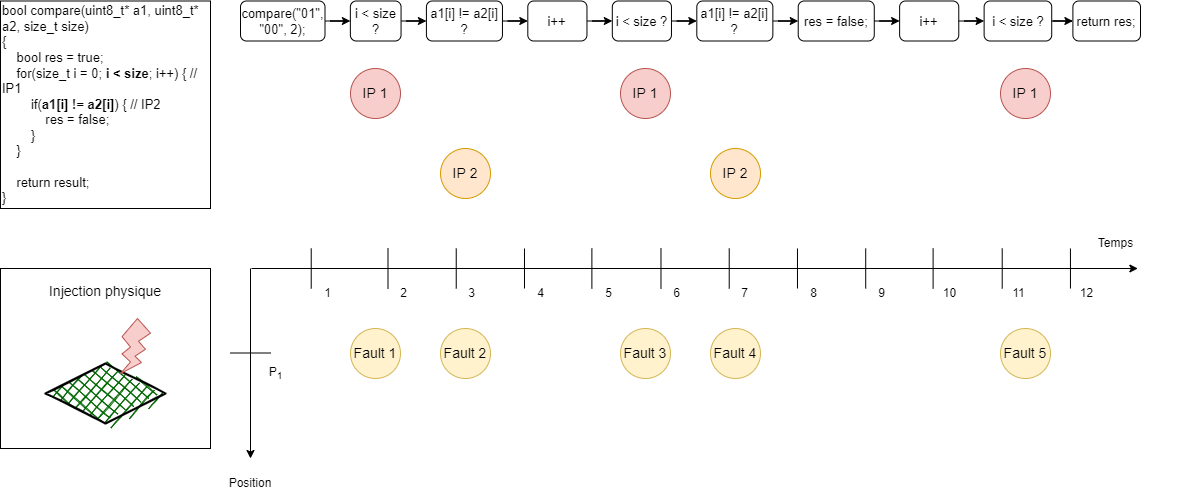
\includegraphics[scale=.41]{ch2-background/img/spatiotemporal.drawio.png}}
                  \caption{Comparaison des fautes sur la fonction compare en inversion de test}
                  \label{fig:soft-hard-compare}
                \end{figure}            
        
            \subsubsection{Persistance temporelle}
                
                BarEl et al. \cite{BarEl/IEEE06} indiquent qu'un circuit peut être sujet à deux types de fautes: les fautes \textbf{permanentes} (destructives) et les fautes \textbf{transitoires}.
                Dans le cas de fautes \textit{transitoires} (ou \textit{provisoires}), la faute a un effet immédiat sur le système en provoquant une mauvaise interprétation d'un signal. Lorsque la faute cesse, le circuit revient ensuite à son état initial.
                A l'inverse, les fautes \textit{destructives} ont un effet permanent sur le système en altérant l'intégrité d'un registre, d'une cellule mémoire ou du circuit par exemple.
                
                En pratique, cette taxonomie au niveau physique est difficile à transposer à un niveau d'abstraction plus élevé. Une faute transitoire peut avoir un effet \textit{permanent} ou \textit{semi-permanent}, sur le programme.
                Par exemple, si une faute transitoire modifie une valeur dans un registre qui est ensuite écrite en mémoire vive (\gls{ram}), alors l'effet de la faute persistera jusqu'à la fin de l'exécution du programme. Dans sa thèse \cite{Brejon/Phd20}, J.-B. Bréjon parle de \textbf{faute persistante} lorsque qu'une faute transitoire a un effet qui persiste au delà de son effet physique sur le circuit. Il cite aussi le cas où une faute transitoire implique une modification d'une instruction du programme chargée en \gls{ram}.
                Dans un cas plus extrême, une faute transitoire peut avoir un effet permanent sur un système, par exemple si la valeur fautée est ensuite utilisée dans un système de mise à jour de micro-programme (firmware updater). La faute aura alors un impact sur le système même après la fin de l'exécution du programme, voire provoquera l'arrêt du système, la faute ayant été répercutée dans la mémoire non volatile.
                On parle aussi de fautes \textit{transitoires répétitives} \cite{Berthome/ARES12} lorsqu'une faute transitoire peut être répétée, par exemple en fautant un bus mémoire plusieurs fois pour introduire plusieurs valeurs invalides successivement.
            
        \subsection{État de l'art des modèles de faute}
        \label{sec:soa-models}
        
            Cette sous-section propose un aperçu des modèles de faute considérés dans la littérature, à la fois par les attaques physiques et par les outils d'analyse. Cet état de l'art est organisé en fonction du niveau de représentation du programme.
            La section \ref{sec:model:physic} présente les modèles au niveau matériel, la section \ref{sec:model:binary} les modèles de faute au niveau de la micro-architecture et du jeu d'instructions, ainsi que des modèles au niveau assembleur et finalement la section \ref{sec:model:source} se concentre sur les modèles au niveau source.
        
            \subsubsection{Modèles au niveau matériel}
            \label{sec:model:physic}
            
                Au niveau physique, l'injection d'une faute introduit une perturbation qui va modifier le fonctionnement du circuit. Le circuit peut consister en des portes logiques, des cellules mémoire ou encore des bascules.
                
                Le modèle de faute considéré à bas niveau est lié à la technique d'injection de fautes utilisée. Certaines techniques comme celles basées sur les ondes électromagnétiques \cite{Maistri/VLSI-SoC14, Dument/FDTC19} ou les impulsions laser \cite{Van/FDTC11, Dutertre/DTIS14} ont une haute précision à l'inverse des glitchs de température \cite{Hutter/ICSCRAA13} par exemple.
                Les caractéristiques des fautes injectées vont alors dépendre des paramètres expérimentaux choisis (moment et position de l'injection, durée et intensité d'un rayonnement etc.).
                
                \begin{table}[ht]
                \centering
                    \begin{tabular}{|l|l|l|l|}
                    \hline
                    Valeur / Granularité & Niveau bit & Niveau byte & Autres plages \\ \hline \hline
                    mise à 0                             & bit-set       & byte set        & set          \\ \hline
                    mise à 1                             & bit-reset     & byte reset      & reset        \\ \hline
                    inversion                            & bit flip   & byte flip       & flip         \\ \hline
                    aléatoire                            & bit ran    & byte ran       & rand    \\    \hline
                    \end{tabular}               
                \caption{Modèle de faute sur les données \label{tbl:bits}}
                \end{table}
                
                Au niveau d'une donnée dans le circuit (dans un bus ou une cellule mémoire par exemple), on distingue souvent les modèles en fonction de la granularité de la plage de bits pouvant être visée et la façon dont la valeur peut être modifiée, comme indiqué dans la table \ref{tbl:bits}.
                La granularité de la faute en donnée peut consister en un seul bit, un octet, une plage contiguë quelconque ou une plage non contiguë de bits.
                Concernant la valeur fautée, on peut distinguer les modèles de mise-à-zéro et de mise-à-un ainsi que l'inversion des bits. 
                Les modèles de type aléatoire permettent de simuler les injections en données sur des mémoires chiffrées où l'attaquant a un contrôle limité sur la valeur qui pourra être injectée. 
            
            \subsubsection{Modèles au niveau architectural et ISA}
            \label{sec:model:binary}
            
                Au niveau architectural, les fautes peuvent être distinguées en fonction de la partie de l'architecture qui est ciblée comme présenté dans la figure \ref{fig:arch-models-scheme}:
                \begin{itemize}
                    \item fautes sur les instructions,
                    \item fautes sur les données (registres, cache, mémoire),
                    \item fautes sur la micro-architecture: pipeline, registres cachés...
                \end{itemize}             
                
                \begin{figure}[ht]
                    \centering
                    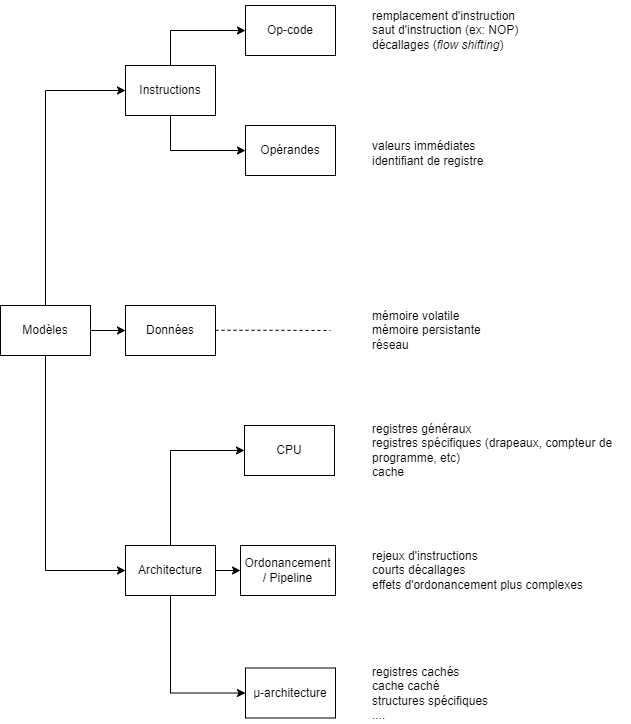
\includegraphics[scale=.56]{ch2-background/img/Modeles Architecture fr.drawio.png}
                    \caption{Classification des modèles au niveau architectural}
                    \label{fig:arch-models-scheme}
                \end{figure}
                    
                \paragraph{}
                Lorsqu'on se place au niveau du jeu d'instructions (\gls{isa}), une modification de bits induit une transformation des instructions ou des données.
                Une faute peut avoir pour effet la modification de l'opérande (les paramètres de l'instruction), de l'opcode (le type de l'instruction) ou les deux.
                
                La figure \ref{fig:armv7-mov-encoding} présente la spécification de l'encodage des trois versions de l'instruction \textit{MOV} dans le jeu d'instructions \textit{ARMv7-M thumb2} \cite{ARMv7/manual}. 
                Les bits correspondant à l'opcode dans l'encodage sont indiqués avec une valeur fixe binaire tandis que les opérandes sont nommées. Les opérandes de la forme \texttt{immX} correspondent à la valeur immédiate (constante) qui sera déplacée et \texttt{rd} correspond au registre de destination. Si ces bits sont changés par une faute, le type de l'instruction restera le même (MOV-TX), mais avec des paramètres différents \cite{Colombier/HOST19}.
                Un cas particulier du remplacement d'instruction est le saut d'instructions\footnote{D'autres types de fautes peuvent toutefois induire un saut d'instruction, comme par exemple la modification du compteur du programme (\gls{pc}).} très largement étudié \cite{Balasch/FDTC11, Kelly/HOST17, Moro/FDTC13}, dans lequel la faute permet d'ignorer l'exécution d'une ou plusieurs instructions (par exemple, en transformant une instruction en instruction \gls{nop})).
                Dans le cas de jeu d'instructions à taille d'instruction variable comme c'est le cas pour \textit{thumb}, la mutation au niveau de l'\textit{op-code} peut jouer sur la taille de l'instruction (en passant d'une instruction de deux à quatre octets ou réciproquement) et peut entraîner une mutation en cascade des instructions interprétées par la suite, et donc un impact significatif sur la structure du reste du programme au niveau binaire. Cette suite de décodage erronés \textit{flow shifting} \cite{Berthome/ARES12} est généralement assez courte en raison d'instructions invalides amenant à un crash du processeur \cite{Shacham/CCS07}.
                
                \begin{figure}[ht]
                    \centering
                    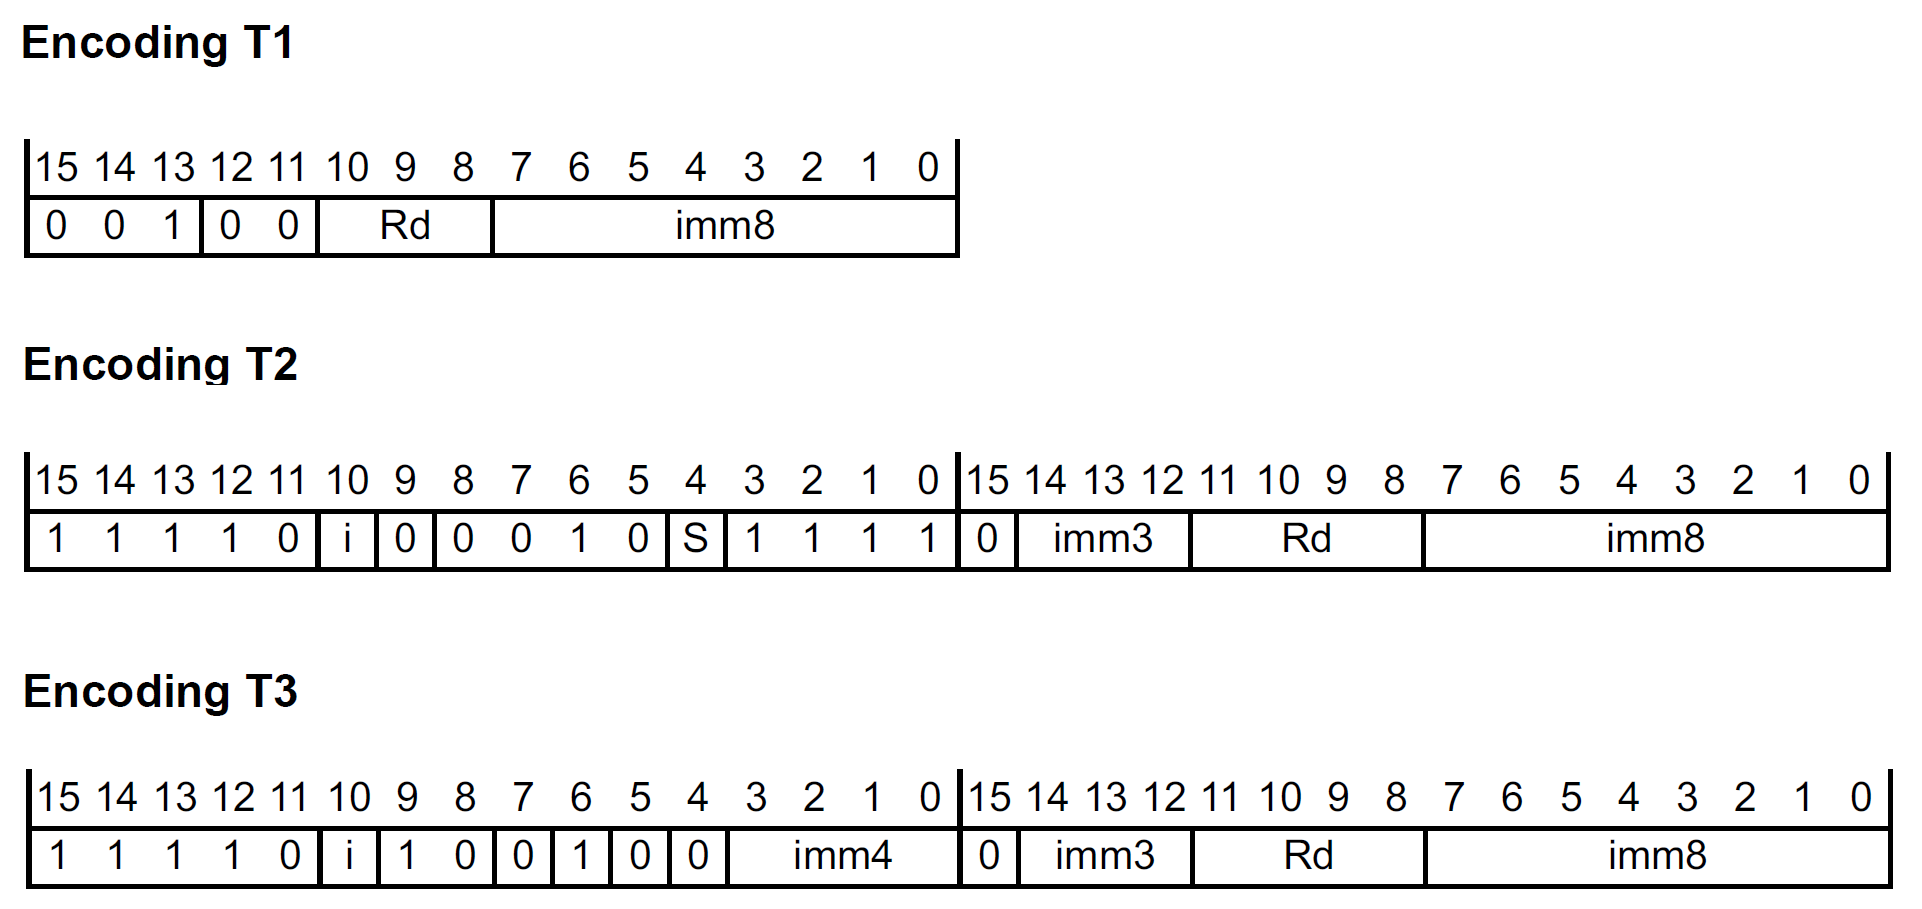
\includegraphics[scale=.32]{ch2-background/img/armv7-encoding.png}
                    \caption{Encodage de l'instruction MOV sur l'architecture ARMv7-M thumb2}
                    \label{fig:armv7-mov-encoding}
                \end{figure}
                
                \paragraph{}
                La modification des données consiste à changer les bits dans un registre du processeur, sur un bus mémoire pendant son transit ou dans la mémoire. La corruption de registre est également un modèle très étudié dans l'analyse au niveau binaire \cite{Blomer/CCS03, Verbauwhede/FDTC11}.
                De la même manière qu'au niveau matériel, différentes valeurs et plages de bits peuvent être considérées en fonction du  modèle de faute comme indiqué dans la figure \ref{tbl:bits}.
                Dans le domaine de la tolérance aux fautes, les modèles étudiés se restreignent souvent à une inversion de bit simple sur la donnée \cite{lu2015llfi, sharma2013towards, van2014evaluating, Georgakoudis/ICHPCNSA17, le2018resilience}. 
                Les modèles considérant la modification de plusieurs bits contiguës voire de fautes indépendantes existent \cite{CERN07}.
                La modification des données peut aussi correspondre à la modification d'une adresse ou de son calcul (comme un index de tableau par exemple).
                
                \paragraph{}
                Au niveau micro-architectural, c'est-à-dire en tirant parti des spécificités de l'architecture interne du processeur et des composants, des modifications plus subtiles peuvent être observées.
                Rivière et al. \cite{Riviere/HOST15} montrent qu'il est possible d'exploiter le tampon de pré-chargement du processeur (\textit{prefetch buffer}) pour annuler son remplissage et ainsi répéter une instruction en ignorant une partie des instructions suivantes.
                Le rejeu d'instruction \cite{Riviere/FPS14} consiste à exécuter deux fois une instruction, par exemple en attaquant la valeur du \gls{pc}, ou de la pipeline du processeur.
                Lorsqu'il s'accompagne du saut de l'instruction suivante, il peut s'assimiler à un remplacement de l'instruction.
                Plus récemment, Laurent et al. proposent des exploitations de fautes sur la micro-architecture, avec notamment des effets sur le processeur non-observables sur le jeu d'instructions \cite{Laurent/ECDSD19, Laurent/DATE19}.
                Par ailleurs, les modèles de faute visant les caches du processeur correspondent à des modèles ciblant la micro-architecture du processeur.
                
            \subsubsection{Modèle au niveau source}
            \label{sec:model:source}
            
                A plus haut niveau, les modèles de faute s'intéressent davantage aux modifications de la logique algorithmique du programme. En fonction de si on se place au niveau du code source ou d'un niveau intermédiaire, la granularité des fautes peut varier.
                La figure \ref{fig:software-models-scheme} présente une classification des modèles de faute au niveau source.
                Deux grandes classes de modèles de faute se dégagent de la littérature: l'\textit{altération des chemins d'exécution} du programme et la \textit{modification des données}. 
                
                \begin{figure}[ht!]\centering
                  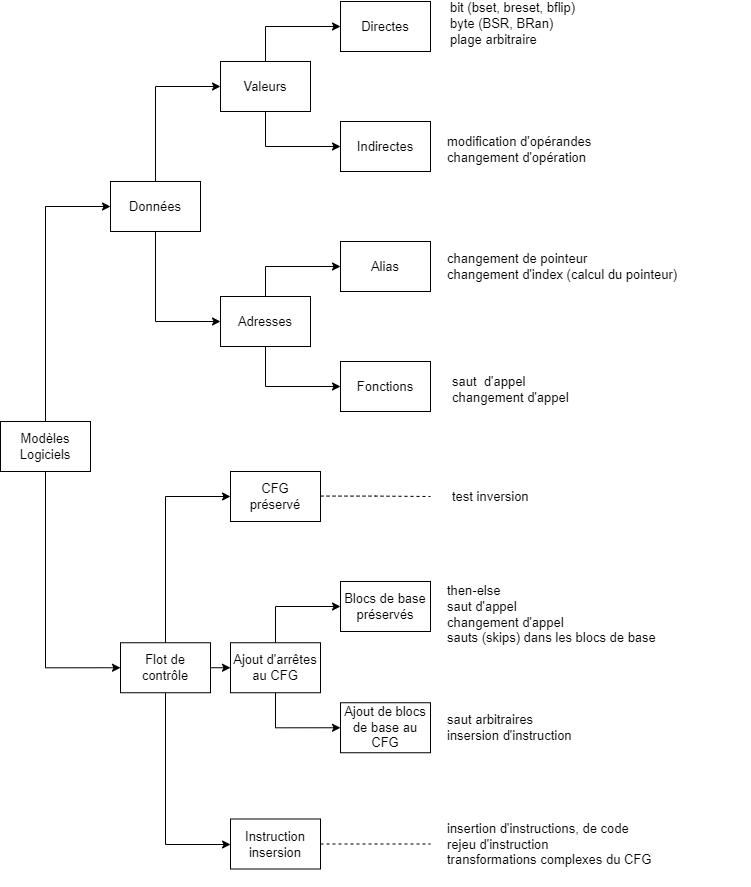
\includegraphics[scale=0.49]{ch2-background/img/Class Logiciel.drawio.png}
                  \caption{Classification des modèles de faute au niveau source}
                  \label{fig:software-models-scheme}
                \end{figure}
            
                L'altération des chemins d'exécution concerne les fautes ayant un effet sur l'intégrité du flot de contrôle \cite{Abadi/TISSEC09, Sayeed/AS19}. Il s'agit de détourner le flot d'exécution de son comportement normal.
                Le \textit{graphe de flot de contrôle} (\gls{cfg}) est une représentation du flot de contrôle du programme correspondant à un graphe orienté. 
                Les nœuds sont des blocs de base qui correspondent à une suite d'instructions atomiques (toujours exécutées en séquence).
                Les arêtes correspondent aux branchements conditionnels et aux sauts.
                Ainsi la figure \ref{fig:software-models-scheme} distingue les modèles axés sur la modification du flot de contrôle en fonction de leur impact sur le graphe de flot.
                
                Le modèle de l'inversion de test \cite{Berthome/ARES12, Potet/ICST14, Dureuil/PPLCC16} consiste à inverser le chemin sélectionné après une opération de branchement conditionnel. 
                Dans \cite{Bouffard/SCRAA11}, Bouffard et al. parviennent à modifier le flot de contrôle d'un programme Java Card\footnote{Plateforme Java minimaliste embarquée pour les cartes à puce.} en attaquant l'adresse de retour d'une fonction.
                Les modèles basés sur le saut d'instructions existent aussi au niveau source \cite{Moro/FDTC13, Potet/ICST14, Barry/CSCS16, Breier/TDSC19}.
                Ils ont généralement une granularité plus faible au niveau logiciel qu'au niveau matériel, comme par exemple dans \cite{lalande}, où Lalande et al. s'intéressent à un modèle de saut d'instructions au niveau du langage C. Il peut aussi s'agir de sauts d'appels de fonction \cite{Dureuil/PPLCC16}.
                Ces modèles attaquant l'intégrité du flot de contrôle sont un sujet important au niveau source, car ils induisent des comportements difficiles à anticiper et peuvent produire des nouveaux chemins dans l'application, que ce soit dans les outils d'analyse de robustesse tels que SmartCM \cite{Machemie/IFS11}, l'évaluation de contre-mesures \cite{Sere/IJSIA11} ou l'introduction de contre-mesures, par exemple à la compilation \cite{Werner/ICSCRAA15}. 
                
                La modification de données s'apparente principalement à la modification des valeurs lues ou écrites dans les variables, ou les valeurs temporaires utilisées pour calculer les expressions (i.e. les registres).
                Breier et al \cite{Breier/TDSC19} étudient l'effet d'un nombre arbitraire d'inversions de bits dans un registre. 
                La modification d'une donnée lors de la lecture en mémoire est également un modèle standard dans l'analyse de robustesse au niveau logiciel \cite{Moro/FDTC13, Berthome/ARES12}. 
                Le modèle d'inversion de bit dans une zone mémoire est aussi fréquemment utilisé dans le domaine de la tolérance aux fautes \cite{Benso/TODAES98, Georgakoudis/ICHPCNSA17}.
                L'attaque \textit{Rowhammer} \cite{Kim/ACM14} qui a été abordée dans le chapitre \ref{chpt:contexte} correspond à une modification de données sur la mémoire.
                
                \paragraph{}                
                La modification de données peut avoir un effet sur le flot de contrôle, par exemple dans le cas d'une faute d'une adresse de retour, d'une adresse de fonction, d'une adresse lors d'un saut arbitraire, et plus généralement lorsqu'une valeur est utilisée par la suite dans une condition ou un saut. 
                A l'inverse, le flot de contrôle peut avoir un effet comparable à une mutation de donnée puisque le flot détourné peut modifier des données différemment du comportement normal du programme.
                Lacombe et al \cite{lacombe2021combining} proposent un modèle visant les expressions au niveau CIL (représentation intermédiaire de l'outil Frama-C), permettant de considérer à la fois les modifications de données arbitraire et les fautes visant le flot de contrôle (avec la mutation de la valeur finale de l'expression dans les conditions). 
                
        \subsection{Classification des modèles au niveau logiciel}
        \label{sec:model-classification}
        
            Les sections précédentes ont présenté les problématiques liées à la mise en relation des modèles de faute à différents niveaux de représentation.
            Celles-ci concernent à la fois la représentativité des modèles étudiés à haut niveau par rapport à la réalité physique, la difficulté de l'observation et de la caractérisation des fautes et la compréhension de leurs effets \cite{Dureuil/CARDIS15, werner2020end}.
            Cette sous-section vise à présenter différentes approches pour classifier les modèles au niveau logiciel ainsi que la difficulté pour faire correspondre des modèles de niveaux différents.
            
            La figure \ref{fig:software-models-scheme} présentée dans la section \ref{sec:model:source} fait une première distinction entre les modèles sur le flot de contrôle et ceux sur les données. 
            La classification des modèles source peut aussi être réalisée en partant de la cible des fautes à bas niveau (instructions, données, registres, pipeline etc.).
            C'est en partie l'approche qui est utilisée dans la figure \ref{fig:arch-models-scheme} présentant les modèles au niveau architectural.
            La modification de données sur des zones différentes de l'architecture implique alors des modèles haut niveaux très variables.
    
            Une autre solution serait de classifier les modèles en fonction de l'inclusion de l'ensemble des fautes pouvant être réalisées. Cela peut être fait en considérant l'espace de faute de chaque modèle ou bien en comparant les comportements obtenus par chaque modèle. Il est par exemple possible de considérer qu'un modèle de mutation de donnée est un sous-ensemble d'un modèle de modification arbitraire de donnée ou encore qu'une inversion de test peut correspondre, en partie, à un cas spécifique du saut d'instruction lorsqu'on se place au niveau de représentation \gls{isa}.
            Cependant, cette approche a ses limites puisque les espaces de fautes de deux modèles peuvent ne pas avoir de relation d'inclusion et selon le niveau de représentation choisi, les relations entre les modèles de faute peuvent être très différentes. 
            La combinaison de modèles de faute et la prise en considération de fautes multiples compliquent encore cette notion d'inclusion\footnote{Par exemple, un modèle de mutation de donnée sur une instruction d'écriture de mémoire (store) peut être simulée par un nombre non borné de mutations de donnée en lecture (load).}.  
            
            Cela illustre la difficulté de faire correspondre des modèles à des niveaux de représentation différents et la question de la légitimité de raisonner à propos de modèles trop bas niveau lorsqu'on considère un programme au niveau logiciel.
            Les programmes doivent faire face à des attaquants très variés, et la définition ainsi que la modélisation des fautes sont des difficultés de l'évaluation de la robustesse d'un programme.
            Les modèles au niveau logiciel visent à être suffisamment génériques pour couvrir un maximum les modèles pouvant effectivement être observés mais sans viser la correspondance exacte avec ces modèles bas niveau et s'orientent plutôt vers la prise en compte de la logique algorithmique du programme. 
                    
    \section{Protection contre les attaques physiques}
    \label{sec:fi-protections}
        
        Afin de lutter contre les attaques physiques, de nombreuses solutions de protections ont été proposées \cite{BarEl/IEEE06, Yuce/HSS18}. 
        Ces protections peuvent prendre des formes variées en fonction du niveau de représentation et du modèle d'attaquant considéré. Cette section vise à donner un court aperçu des protections contre les attaques par injections de faute et les attaques physiques (fautes accidentelles et canaux auxiliaires). 
        Le chapitre \ref{chpt:placement} approfondit les problématiques liées à l'analyse et l'évaluation de protections dans le cadre d'attaques en fautes et présente un état de l'art des protections logicielles existantes dans la littérature.
        
        \begin{defi}
            Une \textit{protection} correspond à toute modification du programme, de l'architecture ou du matériel et de leurs fonctionnements visant à empêcher une attaque d'aboutir, la détecter, la corriger ou la rendre plus difficile à effectuer.
        \end{defi}
        
        \begin{defi}
            Une \textit{contre-mesure} est une protection visant à détecter une attaque afin de pouvoir ensuite la signaler, la corriger ou prendre des mesures comme le redémarrage du système ou sa coupure.
        \end{defi}
        
        Au niveau physique, les protections peuvent prendre la forme de détecteurs surveillant la tension d'alimentation ou la fréquence du circuit \cite{Zussa/DATE14}. 
        Les boucliers actifs (\textit{active shields}) \cite{BarEl/IEEE06} correspondent à un maillage métallique dans lequel les données circulent en continue. Si le maillage est endommagé ou modifié, le circuit ne fonctionne plus.
        Les détecteurs physiques permettent de réagir à une fréquence ou une tension inhabituelle \cite{BarEl/IEEE06}. 
        Les protections visant à limiter la connaissance de l'attaquant en rendant l'observation plus difficile sont très fréquentes dans le domaine des canaux auxiliaires. Parmi les protections physiques de ce type on peut citer le chiffrement de la mémoire \cite{Barenghi/IEEE2012} ainsi que l'ajout d'aléa dans la consommation de courant par exemple \cite{Moro/Phd14} ou encore dans l'ordonnancement des instructions \cite{Wittman/RSA08}.
        
        Au niveau architectural, la tâche de l'attaquant peut être rendue plus ardue en utilisant un encodage pour le jeu d'instructions compliquant attaques: par exemple un encodage différent de \texttt{0} pour l'instruction \gls{nop} est une solution pour se protéger contre les attaques de mise-à-0.
        Des protections par redondance des calculs ou des données peuvent par exemple être obtenues en ayant deux circuits de calcul dans le processeur ou l'\gls{alu}, qui comparent ainsi leur résultats, cette redondance pouvant être étendue à $n$ circuits redondants \cite{BarEl/IEEE06}.  
        
        Au niveau logiciel, les protections peuvent être appliquées sur toute la couche logicielle. On distinguera les protections appliquées en tant que transformation du programme et celles appliquées au niveau du système (système d'exploitation par exemple). 
        Les protections qui effectuent une transformation du programme source peuvent être appliquées à plusieurs niveaux de représentation du programme. 
        L'utilisation d'instructions idempotentes afin de se protéger contre les sauts d'instructions \cite{Moro/Phd14} a été proposée au niveau assembleur tandis que des protections ont été proposées au niveau du langage C \cite{lalande} ou lors de la compilation \cite{Barry/CSCS16, Proy/TACO17}. 
        Certaines approches visent la protection de l'intégrité du flot de contrôle par des mécanismes de signature de blocs ou de fonctions \cite{Oh/TR02, Reis/ISCCO05, Ferriere/LLVM19} ou encore par l'utilisation d'une \textit{pile cachée} \cite{Dureuil/CARDIS15} par exemple.
        L'utilisation de booléens endurcis visent à compliquer la tâche de l'attaquant d'une façon similaire à l'exemple de l'encodage du \gls{nop} pour le niveau architectural.
        
        Une partie des protections physiques, notamment celles basées sur la redondance des calculs ou de la mémoire, ou le chiffrement de celle-ci, peuvent être implémentées à plus haut niveau. Cependant, les protections logicielles peuvent être limitées par rapport à leurs équivalents physiques. En général, les systèmes sont protégés en combinant différents niveaux de protection \cite{Yuce/HASSP16}.
        
        \begin{figure}[htb]\centering
          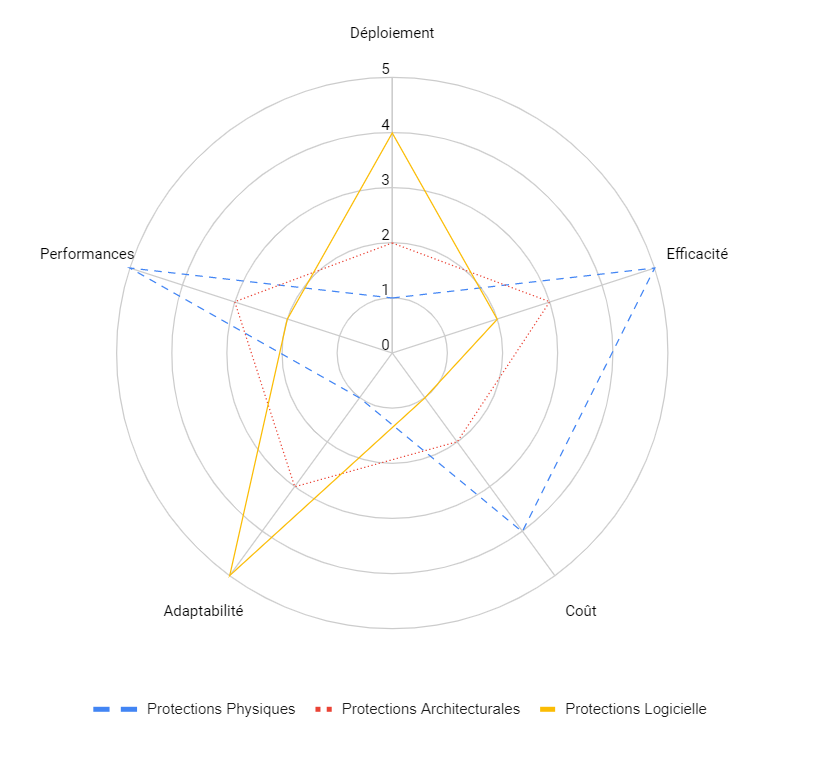
\includegraphics[scale=.58]{ch2-background/img/ch2-protections-caracs.png}
          \caption{Caractéristiques des protections à différents niveaux}
          \label{fig:ch2-protections}
        \end{figure}
        
        \paragraph{} La figure \ref{fig:ch2-protections} compare certaines caractéristiques des protections en fonction du niveau auquel elles sont introduites: 
        \begin{itemize}
            \item \textit{Portabilité}: capacité à s'adapter à une architecture ou une application donnée.
            \item \textit{Déploiement}: facilité de mise-à-jour de la protection.
            \item \textit{Efficacité}: capacité à protéger.
            \item \textit{Coûts}: coûts de développement et de mise en place.
            \item \textit{Performance}: taille du code, consommation mémoire et temps d'exécution ajoutés.
        \end{itemize}         
        
        Les protections physiques permettent de protéger l'ensemble des programmes d'un composant mais sont plus coûteuses à mettre en place et ne peuvent pas être modifiées une fois que le produit est déployé (une carte à puce par exemple). 	\`A l'inverse, les protections logicielles peuvent être ajoutées à l'aide de mises-à-jour logicielles. 
        Les protections de plus haut niveau peuvent ainsi être adaptées aux protections disponibles à plus bas niveau sur lesquelles elles peuvent s'appuyer.  
        Les protections bas niveau peuvent protéger des modules du système qui ne sont pas accessibles au niveau logiciel, mais ne peuvent pas être adaptées à un programme ou une pile logicielle particulière et visent une protection générique du composant.
        
        La protection contre les attaques en fautes est fortement compliquée contre les attaques en \textit{fautes multiples}.
     
    \section{Les fautes multiples}
    \label{sec:multi-fault}
        
        La littérature récente contient des exemples d'attaques en fautes multiples \cite{kim2007fault, Barenghi/IEEE2012, Natella/ACM16, SSTIC20}.
        
        Les fautes multiples rendent le processus de développement d'un programme sécurisé d'autant plus difficile que le nombre de configurations de fautes possibles sur un programme croît rapidement. Cette explosion combinatoire complique l'expertise humaine et l'analyse des outils pour l'évaluation de robustesse.
        De plus, la combinaison de plusieurs modèles de faute doit être considérée et rend plus complexe la protection et l'analyse de robustesse.
        
        Dans le cas de la protection d'un système, la présence de fautes multiples complique également la tâche. En effet, si plusieurs fautes peuvent être injectées, alors une protection peut elle-même être visée par une première faute pour rendre possible la seconde. Dans la fonction \textit{compare} du programme \texttt{verify\_pin} présentée dans le listing \ref{lst:verifyPIN-BAC-LC}, une première injection peut éviter la boucle \texttt{for} (par exemple avec une inversion de la condition \texttt{i < size}) et une seconde peut inverser la condition \texttt{if(i != size) killcard()} afin d'éviter la contre-mesure.
            
            
\lstset{caption={Compteur de boucle sur la fonction \texttt{compare}},label=lst:verifyPIN-BAC-LC}
\begin{lstlisting}     
bool compare(uint8_t* a1, uint8_t* a2, size_t size)
{
    bool result = true;
    for(size_t i = 0; i < size; ++i)
        if(a1[i] != a2[i])
            result = false;
    
    if(i != size) // Protection
        killcard();
        
    return result;
}
\end{lstlisting}
    
        Cette possibilité d'attaquer les protections elles-mêmes, d'autant qu'une grande partie de la littérature propose des contre-mesures visant principalement des fautes uniques, rend l'évaluation et la conception de protections plus complexes dans le contexte des fautes multiples.
        La prise en compte des fautes multiples pour l'analyse de robustesse de programme et pour l'analyse de protections est une problématique à laquelle cette thèse vise à répondre sur deux aspects:
        
        \begin{itemize}
            \item Maîtriser l'exploration des exécutions en multi-fautes malgré l'explosion combinatoire des chemins (chapitres \ref{chpt:lazart} et \ref{chpt:lazart-implem}).
            \item Aider à l'analyse et au placement des contre-mesures dans un contexte multi-fautes (chapitres \ref{chpt:placement} et \ref{chpt:ccpo}).
        \end{itemize}
        
        Avant de s'intéresser à l'outil Lazart, la suite de se chapitre se termine par une analyse des outils existants.
            
        \section[État de l'art des outils d'analyse de robustesse]{État de l'art des outils d'analyse de robustesse pour l'injection de faute}
    \label{sec:soa-tools}

        Cette section propose un aperçu des outils existants pour l'évaluation de robustesse dans le cadre de la tolérance aux fautes et des attaques par injection de fautes. Elle vise aussi à proposer un ensemble de critères pour la comparaison de ces outils. L'état de l'art des outils et des techniques d'analyse pour l'injection de fautes a déjà fait l'objet de plusieurs articles de recherche \cite{kooli2014survey, Given/ICESS17, gangolli2022systematic} et de surveys \cite{Christofi/Phd13, Dureuil/Phd16, Heydemann/HDR17}. Les outils visant la tolérance aux fautes sont également considérés.        
        
        \begin{figure}[ht]\centering
          
\includegraphics[scale=.45]{ch2-background/img/plan-soa-tools.drawio.png}
          \caption{Organisation et périmètre de l'état de l'art}
          \label{fig:soa-tools-scheme}
        \end{figure}
         
        La suite de cette section s'organise comme suit. La sous-section \ref{sec:soa-tools-carac} présente différents critères qui seront considérés pour la comparaison des outils. L'état de l'art est organisé en fonction de la technique d'analyse employée comme montré dans la figure \ref{fig:soa-tools-scheme}. Les sous-sections \ref{sec:soa-tools-test} et \ref{sec:soa-tools-formal} présentent respectivement les méthodes basées sur les tests et celles reposant sur les méthodes formelles.
        Enfin, la sous-section \ref{sec:soa-tools-conclusion} conclut cette section.
        
        \subsection{Caractéristiques des outils}
        \label{sec:soa-tools-carac}
     
            Différentes caractéristiques peuvent être considérées lorsqu'on s'intéresse à un outil d'analyse concernant les attaques en fautes.
            La figure \ref{fig:soa-tools-conclusion} présente une classification d'un ensemble de caractéristiques issus de la littérature et qui seront considéré dans cette section :
            
            \begin{figure}[hbt]\centering
              
\includegraphics[scale=.55]{ch2-background/img/tools-carac.drawio.png}
              \caption{Classification des caractéristiques pour les outils d'analyse de robustesse contre les fautes}
              \label{fig:soa-tools-conclusion}
            \end{figure}
            
            \begin{itemize}
                \item[$\bullet$] \textbf{C1} Caractéristiques opérationnelles:
                \begin{itemize}
                    \item[-] \textit{Coûts}: regroupe les coûts liés au développement de l'outil en termes de moyens humains et de matériel ainsi que le niveau d'expertise requis par l'utilisateur pour l'utilisation de l'outil. 
                    \item[-] \textit{Généricité}: détermine à quel point l'outil est spécifique à un matériel ou une architecture donnée (on parlera à l'opposé de \textit{spécificité}).
                    \item[-] \textit{Automatisation}: niveau d'intervention de l'utilisateur requis.
                    \item[-] \textit{Expertise}: niveau d'expertise de l'utilisateur dans le domaine étudié ou la méthode d'analyse utilisée par l'outil. 
                    \item[-] \textit{Vitesse}:  comprend la vitesse d'exécution de l'outil pour une analyse ou encore le temps de mise en place nécessaire entre deux expérimentations. 
                    \item[-] \textit{Passage à l'échelle}: capacité de l'outil à analyser des programmes / systèmes complexes.
                    \item[-] \textit{Destructivité}: possibilité d'endommager le système étudié par l'analyse.
                \end{itemize}
                
                \item[$\bullet$] \textbf{C2} Caractéristiques liées à la modélisation:
                \begin{itemize}
                    \item[-] \textit{Niveau de représentation}: niveau de représentation de l'analyse (à ne pas confondre avec le niveau d'implémentation de l'outil).
                    \item[-] \textit{Modèle d'attaque}: modèles de faute supportés, support des fautes multiples et objectifs d'attaque étudiés.
                    \item[-] \textit{Contexte d'analyse}: 
                    \begin{itemize}
                        \item[$\circ$] \textit{Cible de l'analyse}: le type de système visé par l'analyse (programme, application, circuit, machines distribuées...).
                        \item[$\circ$] \textit{Domaine}: attaques en fautes, canaux auxiliaires ou fautes accidentelles.
                    \end{itemize}
                \end{itemize}                
                
                \item[$\bullet$]\textbf{C3} Caractéristiques liées aux résultats:
                \begin{itemize}
                    \item[-] \textit{Représentativité}: représentativité des résultats obtenus par rapport à une véritable attaque. 
                    \item[-] \textit{Reproductibilité}: détermine si les résultats obtenus peuvent facilement être reproduits. 
                    \item[-] \textit{Observabilité}: correspond à la capacité de la méthode d'observer l'effet des fautes injectées. 
                    \item[-] \textit{Contrôlabilité}: détermine le contrôle qu'offre la méthode sur les fautes qui seront injectées.
                    \item[-] \textit{Complétude}: couverture des exécutions fautées par l'analyse.
                    \item[-] \textit{Métriques}: métriques produites par l'outil.
                \end{itemize}
                
                \item[$\bullet$]\textbf{C4} Caractéristiques spécifiques: sous-classe de la technique d'analyse, technique d'implémentation.
            \end{itemize}
            
            Les caractéristiques suivantes, correspondant à des combinaisons de caractéristiques, seront aussi étudiées :
            \begin{itemize}
                \item \textit{Performance} (\textbf{C1}): passage à l'échelle et vitesse.
                \item \textit{Mise-en-place} (\textbf{C1}): regroupe les coûts lié au développement de l'outil en termes de moyens humains et de matériel et la destructivité.
                \item \textit{Accessibilité} (\textbf{C1}\&\textbf{C3}): regroupe les caractéristiques de l'expertise requise pour l'utilisateur, l'automatisme et la contrôlabilité.
            \end{itemize}
            
        \subsection{Outils basés sur le test}
        \label{sec:soa-tools-test}
        
            Cette sous-section s'intéresse aux outils basés sur le test, c'est-à-dire qui effectuent une sous-approximation des exécutions.
            Cette classe regroupe un grand nombre de techniques et d'outils:
            \begin{itemize}
                \item L'\textit{injection physique} (section \ref{sec:soa-tools-physic}) qui correspond à l'expérimentation en attaquant physiquement le système.
                \item L'\textit{injection logicielle} (section \ref{sec:soa-tools-swifi}) qui englobe tous les outils émulant l'effet des fautes physiques au niveau logiciel.
                \item La \textit{simulation}\footnote{Une partie de la littérature utilise le terme \textit{simulation} par opposition aux méthodes formelles \cite{kooli2014survey, Heydemann/HDR17}. Dans la suite de ce manuscrit, le mot \textit{simulation} ne sera pas employé en ce sens, parlant à la place d'\textit{outils basés sur les tests}.} (section \ref{sec:soa-tools-simu}) qui correspond aux outils exécutant le programme dans un simulateur dans lequel les fautes sont injectées.
            \end{itemize}        
        
            \subsubsection{Injection physique}
            \label{sec:soa-tools-physic}
            
                Une méthode d'injection de fautes physique (laser, glitches...) permet d'étudier le comportement du système soumis à des fautes. 
                Le terme \textit{injection de faute} a d'ailleurs émergé dans la littérature avant l'apparition des attaques par injection de fautes pour désigner des plateformes telles que MESSALINE \cite{Arlat/TSE90} ou encore RIFLE \cite{Madeira/DCC94}.
                Toute technique d'attaque par faute peut théoriquement être utilisée comme protocole de test physique pour un circuit.  
                
                \begin{figure}[hbt]\centering
                  
\includegraphics[scale=.45]{ch2-background/img/advantages-physics.drawio.png}
                  \caption{Caractéristiques de l'injection physique}
                  \label{fig:soa-tools-scheme-physic}
                \end{figure}
                
                La figure \ref{fig:soa-tools-scheme-physic} résume les avantages et inconvénients de ce type de techniques d'analyse. 
                L'indication $CI$ fait référence aux classes de caractéristiques présentées précédemment.
                L'injection physique à l'avantage d'obtenir des résultats très représentatifs sur la robustesse du programme puisque la faute est injectée directement sur le système à analyser et n'inclut donc pas d'étape intermédiaire ou d'abstraction pouvant fausser les résultats.
                L'observation et la caractérisation de la propagation des fautes observées sont difficiles et la mise en place d'un système d'observation peut introduire une perte de précision \cite{Faurax/Phd09, kooli2014survey}.
                
                La mise en place de tels bancs de test peut s'avérer coûteuse en fonction de la technique d'injection de fautes utilisée.
                Ces méthodologies d'analyse par injection physique sont souvent très spécifiques au système étudié par rapport à des approches plus haut niveau.
                De plus, certaines techniques d'injections destructrices peuvent endommager l'appareil étudié.
                Cependant, ces méthodes d'injections physiques sont utilisées pour la certification des composants sécurisés afin de démontrer la faisabilité d'une attaque.               
            
            \subsubsection{Injection au niveau logiciel (SWIFI)}
            \label{sec:soa-tools-swifi}
            
                Une autre technique très largement utilisée est la reproduction au niveau logiciel des fautes, ou de l'effet causé par des fautes au niveau de représentation considéré. 
                Cette technique désignée \gls{swifi} a émergé dès la fin des années 1980 \cite{Segall/FTCS88, Kanawati/FTCS92, Kao/TSE93} dans le milieu des fautes accidentelles pour ensuite se développer dans le domaine des attaques par injection de fautes jusqu'à aujourd'hui \cite{Georgakoudis/ICHPCNSA17}. 
                
                \paragraph{}         
                \gls{fiat} \cite{Segall/FTCS88} est l'un des premiers outils de type \gls{swifi} et a été proposé en 1988. Il vise l'analyse de systèmes distribués.
                Les fautes autorisées sont décrites par l'utilisateur à l'aide d'un langage spécifique et sont ensuite générées lors de la campagne d'expérimentation. Cet outil a notamment été utilisé pour analyser des fautes de type mise-à-zéro et mise-à-un d'octets et l'inversion de deux bits complémentaires \footnote{C'est-à-dire deux bits de valeurs différentes, afin d'éviter d'être détecté par un code correcteur d'erreur simple.} \cite{Barton/TC90}.   
                \gls{fine} \cite{Kao/TSE93}, est une plateforme d'analyse qui considère à la fois les fautes physiques et les fautes liées à des erreurs d'implémentation ou de conception logicielle, et qui vise à étudier la propagation des fautes dans un système d'exploitation.
                L'outil injecte les fautes au niveau logiciel à l'aide d'un noyau UNIX modifié traçant l'exécution et proposant des appels systèmes supplémentaires.
                Les fautes matérielles consistent en une mutation de données dans la mémoire, les registres ou les bus. 
                Les fautes logicielles sont implémentées en tant que modifications du programme binaire et incluent: données mal initialisées, assignation incorrectes, vérifications des cas d'erreurs incomplètes ou encore mauvaise sortie du programme.
                L'outil vise aussi à étudier comment les erreurs se propagent entre les différentes machines et les différents niveaux.
    
                L'outil \gls{define} \cite{Kao/FTPDS94} est une évolution de \gls{fine} qui supporte l'injection dans un système distribué. Celui-ci permet l'injection dans chaque machine, dans n'importe quelle application en mode utilisateur ou superviseur. 
                En plus des appels systèmes rajoutés et de la modification de l'image binaire du programme déjà utilisées dans \gls{fine}, \gls{define} utilise un handler modifié d'interruptions de l'horloge matérielle afin de contrôler l'injection des fautes dans les bus et la mémoire.
                Des expérimentations ont été menées sur un ensemble de 7 machines SunOS pouvant être fautées, l'une d'entre elles étant utilisée comme serveur. Les auteurs constatent que les erreurs sur le serveur se révèlent plus critiques en général que les fautes sur le client. 
                
                \gls{exfi} \cite{Benso/TODAES98} est un environnement d'injection de fautes qui utilise le \textit{trap execution mode} des microprocesseurs pour l'injection de fautes.
                Ainsi, \gls{exfi} ne nécessite pas de matériel spécialisé (comme FERRARI \cite{Kanawati/FTCS92} par exemple) ou la présence d'un système d'exploitation (comme les outils utilisant des traps logicielles type \gls{fine}).
                Une passe est utilisée pour réduire cet ensemble de fautes en fonction de règles spécifiques permettant d'écarter certaines fautes sans perdre en précision. 
                Ces règles visent à écarter les fautes qui n'auraient pas d'effet sur le système, seraient forcément détectées par un mécanisme de détection d'erreur et celles dont le comportement est déjà couvert par une autre faute de la liste.
                \gls{exfi} supporte un modèle de fautes temporaires de type bit-flip pouvant cibler les instructions, la mémoire et les registres.
                Une faute est caractérisée par le nombre d'instructions depuis le démarrage de l'application.
                
                \gls{llfi} \cite{Thomas/SELSE13, Lu/SQRS15}, proposé en 2013, est un outil pour la tolérance aux fautes travaillant sur la représentation intermédiaire \gls{llvm}.
                Celui-ci instrumente le programme à analyser et génère un exécutable pour l'injection de fautes et un exécutable de profilage déterminant quelles fautes vont être injectées.
                \gls{llfi} modélise des inversions de un ou deux bits et vise une douzaine d'instruction comprenant le calcul d'adresse (\texttt{load} et \texttt{store}) ou encore les opérations arithmétiques (\texttt{mul}, \texttt{fmul} etc.).
                L'outil ne considère que les fautes \textit{activées}, c'est-à-dire lorsque la donnée fautée est lue par le programme avant d'être écrasée par une autre instruction.
                Les auteurs constatent sur leurs expérimentations que certaines instructions (comme les instructions de comparaison)
                sont moins sensibles aux fautes que d'autres et que deux inversions augmentent le risque de crash sans augmenter le nombre d'erreurs de calcul non détectées.
    
                REFINE \cite{Georgakoudis/ICHPCNSA17} est une approche basée sur l'injection de fautes à la compilation qui vise à modéliser plus finement des comportements qui sont difficiles à capter au niveau d'une représentation intermédiaire (comme par exemple les prologues / épilogues de fonctions qui sont abstraits par l'IR LLVM).
                REFINE se situe dans le backend du compilateur et a ainsi accès aux instructions spécifiques (au prix de la portabilité).
                L'outil se place ainsi après toutes les passes d'optimisation afin d'éviter que le code injecté puisse être transformé par le compilateur. 
                REFINE se concentre sur un modèle de mutation d'opcode et d'opérande, ignorant les opcodes invalides.
                Les auteurs comparent leur approche à celle de \gls{llfi} qui s'applique également au niveau de l'IR \gls{llvm} et PINFI (qu'ils ont modifiés) qui travaille au niveau binaire sur différents programmes de calcul haute performance (\gls{hpc}).
                Ils indiquent que les performances et la précision de REFINE sont meilleures que celles de \gls{llfi} et égalent, voire dépassent dans certains cas, celles de PINFI. 
            
                \centerline{}
                \begin{table}[hbt]
                    {\tiny
                    \begin{center} 
                    \setlength\tabcolsep{4pt}
                    \begin{tabular}{|l|l|c|c|c|c|c|c|}
                    \hline
                    \multicolumn{1}{|c|}{Outil} & \multicolumn{1}{c|}{Niveau} & Technique & Modèle & Fautes & Cible & Oracle & FI \\ \hline
                    \begin{tabular}[c]{@{}l@{}}FIAT \\ \cite{Segall/FTCS88}\end{tabular} & Physique & \begin{tabular}[c]{@{}c@{}}materiel, OS\\ spécialisé\end{tabular} & \begin{tabular}[c]{@{}c@{}}mémoire\\ registres\\ communication\end{tabular} & 1 & \begin{tabular}[c]{@{}c@{}}système\\ distribué\end{tabular} & SDC & Non \\ \hline
                    \begin{tabular}[c]{@{}l@{}}Ferrari \\ \cite{Kanawati/FTCS92}\end{tabular} & Physique & \begin{tabular}[c]{@{}c@{}}software-trap\\ (syscall)\\ materiel spécialisé\end{tabular} & \begin{tabular}[c]{@{}c@{}}mémoire, registre\\ remplacement inst.\\ fautes permanentes\end{tabular} & 1 & \begin{tabular}[c]{@{}c@{}}système\\ distribué\end{tabular} & SDC & Non \\ \hline
                    \begin{tabular}[c]{@{}l@{}}DEFINE \\ \cite{Kao/FTPDS94}\end{tabular} & UNIX & \begin{tabular}[c]{@{}c@{}}kernel modifié\\ interrupt modifiées\end{tabular} & \begin{tabular}[c]{@{}c@{}}CPU (ALU, cache,\\ decoder, reg, bus), \\ communication\\ fautes de design\end{tabular} & 1 & \begin{tabular}[c]{@{}c@{}}système\\ distribué\end{tabular} & SDC & Non \\ \hline
                    \begin{tabular}[c]{@{}l@{}}Xception \\ \cite{Carreira/IEEE98}\end{tabular} & CPU & \begin{tabular}[c]{@{}c@{}}fonctionnalité\\ CPU\end{tabular} & \begin{tabular}[c]{@{}c@{}}flips, sa1, sa0, bit mask\\ CPU registre bus\end{tabular} & 1 & application & SDC & Non \\ \hline
                    \begin{tabular}[c]{@{}l@{}}EXFI \\ \cite{Benso/TODAES98}\end{tabular} & µkernel & software-trap & \begin{tabular}[c]{@{}c@{}}bitflip\\ (mem / reg)\end{tabular} & 1 & application & SDC & Non \\ \hline
                    \begin{tabular}[c]{@{}l@{}}LLFI \\ \cite{Thomas/SELSE13}\end{tabular} & LLVM & compilation & \begin{tabular}[c]{@{}c@{}}flip ALU\\ store / load\end{tabular} & 1 & application & SDC & Non \\ \hline
                    \begin{tabular}[c]{@{}l@{}}REFINE \\ \cite{Georgakoudis/ICHPCNSA17}\end{tabular} & LLVM & compilation & \multicolumn{1}{l|}{bit-flip sur opérandes} & 1 & \multicolumn{1}{l|}{\begin{tabular}[c]{@{}l@{}}application\\ (HPC)\end{tabular}} & SE & Non \\ \hline
                    \end{tabular}
                \end{center}
                }       
                \caption{Comparaison de quelques outils de type SWIFI \label{tbl:tools-swifi}}
                \end{table}

                \paragraph{}
                La table \ref{tbl:tools-swifi} présente une comparaison de quelques outils de type \gls{swifi}.
                La colonne \textit{Niveau} indique le niveau d'abstraction auquel se place l'outil.
                La colonne \textit{Technique} correspond à la méthode utilisée pour émuler les fautes au niveau logiciel.
                La colonne \textit{Modèle} précise les modèles de faute supportés et la colonne \textit{Faute} la limite de faute pour les attaques.
                La colonne \textit{Cible} correspond au type de système étudié par l'outil (système distribué, application etc.).
                La colonne \textit{Oracle} indique le type de propriété de sécurité ou de sûreté étudiée par l'outil. Ici \textit{SDC} fait référence aux corruptions silencieuses de données.
                Enfin, la colonne \textit{FI} détermine si l'outil vise le milieu des attaques par injection de fautes ou celui des fautes accidentelles (ici tous).
                
                La figure \ref{fig:soa-tools-scheme-swifi} résume les avantages et inconvénients des outils \gls{swifi} comparés aux méthodes d'injection physiques. L'injection logicielle est généralement moins coûteuse, plus facile à mettre en place et plus générique.
                L'observabilité est également supérieure avec les approches d'injection logicielle, qui peuvent tirer partie de certaines technologies comme les exceptions matérielle (\gls{exfi}) \cite{Benso/TODAES98}.
                
                \begin{figure}[htpb]\centering
                  
\includegraphics[scale=.41]{ch2-background/img/advantages-swifi.drawio.png}
                  \caption{Caractéristiques des méthodes SWIFI comparées à l'injection physique}
                  \label{fig:soa-tools-scheme-swifi}
                \end{figure}
                
                La sur-couche logicielle pour émuler la faute offre une représentativité moindre par rapport à l'injection physique et peut aussi ajouter une surcharge qui diminue les performances. Cette perte de précision dépend de la technique d'injection logicielle utilisée et des optimisations ont été développées qu'il s'agisse de représentativité ou de performance \cite{Lu/SQRS15, Georgakoudis/ICHPCNSA17}.
    
            \subsubsection{Outils basés sur la simulation}
            \label{sec:soa-tools-simu}
            
                La simulation désigne les outils qui effectuent une exécution sur un système simulé, sans exécuter directement sur le matériel étudié. 
                Les caractéristiques de l'outil dépendent alors en grande partie de la modélisation du système dans le simulateur.
                
                \paragraph{} 
                Depend \cite{Goswami/TC97} est un simulateur qui vise à prendre en compte les interactions entre les différents composants d'un système complexe en cas de fautes accidentelles.
                L'outil modélise le système en C++ afin de simuler des fautes au niveau des portes logiques. 
                Depend est capable de simuler des fautes sur la mémoire (bit-flip) et dans les communications (paquet perdu, corruption...). Les fautes sont décrites par l'utilisateur en C++ également.
                
                SINJECT \cite{Zarandi/DFTVS03} est un outil qui analyse la robustesse face aux fautes accidentelles au niveau de la représentation \gls{vhdl} et Verilog. 
                Il permet d'injecter un large nombre de fautes physiques au niveau des données et du circuit. Ceux-ci sont introduits dans le système Verilog à partir d'une description utilisateur. L'injection en \gls{vhdl} est faite avec la technique mutant-saboteurs.
                L'outil profite du mode combiné \gls{vhdl}/Verilog permettant de profiter de la représentativité de Verilog et de la description \gls{vhdl}.
                SINJECT s'intéresse à des objectifs d'attaque de tolérance aux fautes sur les traces simulées.
                
                \gls{pafi} \cite{Faurax/CSS06, Faurax/Phd09} est un outil étudiant les fautes au niveau du circuit utilisant la modélisation Verilog et \gls{vhdl}. 
                Il vise à vérifier l'absence de fuite de données secrètes dans le cadre d'attaques en multi-fautes au niveau circuit.
                L'outil s'appuie sur le simulateur Cadence NCSim (un outil propriétaire de STMicroelectronics) et utilise le fichier de commandes du simulateur pour contrôler les fautes à injecter.
                Une pondération basée sur des critères définis en fonction du modèle de faute permet de sélectionner les fautes à simuler (bit-flip sur les bascules ou faute sur les délais dans le circuit), ce qui permet un meilleur passage à l'échelle en multi-fautes.
                Par ailleurs, l'outil prend en compte les mécanismes de détection et indique les faux-positifs, faux-négatifs, attaques non détectées et attaques détectées.
                L'outil se veut extensible et générique en proposant un moyen de définir le modèle de circuit et les modèles de faute.
                
                \begin{sloppypar}   
                Celtic \cite{Dureuil/Phd16, Werner/Phd22} est un simulateur au niveau binaire développé en C++ qui permet de simuler des fautes au niveau de l'\gls{isa} et de l'architecture.
                Celtic supporte les fautes comme le saut d'instruction, la corruption du cache d'instruction \cite{Riviere/HOST15} et les attaques sur les données sur les registres, la mémoire et le décodage des instructions. L'outil supporte également les fautes multiples, ceci étant facilité par la parallélisation des simulations.
                L'objectif d'attaque est exprimé dans le programme et évalué pour chaque trace simulée afin de récupérer les attaques réussies.
                Celtic propose un langage de spécification d'architecture (GISL) permettant d'adapter facilement l'outil à différentes architectures. 
                \end{sloppypar}   
            
                \begin{table}[h]
                {\tiny
                \begin{center}                
                \setlength\tabcolsep{3.9pt}
                    \begin{tabular}{|l|l|l|l|l|l|l|l|l|}
                    \hline
                    Outil & Niveau & Implem & Simu type & Modèle & Fautes & Cible & Oracle & FI \\ \hline
                    FOCUS \cite{Choi/TC92} & Physique & VLSI & externe & porte logiques & X & \begin{tabular}[c]{@{}l@{}}systèmes\\ distribués\end{tabular} & SDC & Non \\ \hline
                    Depend \cite{Goswami/TC97} & \begin{tabular}[c]{@{}l@{}}Circuit\\ µ-arch\end{tabular} & C++ & intégrée & \begin{tabular}[c]{@{}l@{}}circuit\\ communication\\ mem.\end{tabular} & 1 & \begin{tabular}[c]{@{}l@{}}systèmes\\ distribués\end{tabular} & SDC & Non \\ \hline
                    SINJECT \cite{Zarandi/DFTVS03} & \begin{tabular}[c]{@{}l@{}}Verilog /\\ VHDL\end{tabular} & \begin{tabular}[c]{@{}l@{}}Verilog /\\ VHDL\end{tabular} & intégrée & circuit & 1 & application & SDC & Non \\ \hline
                    PAFI  \cite{Faurax/CSS06} & Circuit & \begin{tabular}[c]{@{}l@{}}Verilog /\\ VHDL\end{tabular} & externe & \begin{tabular}[c]{@{}l@{}}bit-flip\\ délais\end{tabular} & X & \begin{tabular}[c]{@{}l@{}}Verilog /\\ VHDL\end{tabular} & \begin{tabular}[c]{@{}l@{}}SC\\ exploit-\\ abilité\\ blocage\end{tabular} & Oui \\ \hline
                    CELTIC  \cite{Werner/Phd22} & x86 & C++ & intégrée & \begin{tabular}[c]{@{}l@{}}data (reg, mem)\\ cache, saut, rejeu\end{tabular} & X & x86 & \begin{tabular}[c]{@{}l@{}}oracle\\ logiciel\end{tabular} & Oui \\ \hline
                    \end{tabular} \end{center}
                }            
                \caption{Comparaison de quelques outils de simulation \label{tbl:tools-simu}}
                \end{table}

                La table \ref{tbl:tools-simu} présente une comparaison de plusieurs outils de simulation.
                Les colonnes \textit{Niveau}, \textit{Modèle}, \textit{Cible}, \textit{Oracle} et \textit{FI} ont la même signification que pour la table des outils \gls{swifi}. 
                La colonne \textit{Fautes} indique la limite de faute, le symbole "X" indiquant le support des fautes multiples.
                La colonne \textit{Implem} correspond au niveau auquel l'outil est implémenté (ce qui peut être différent du niveau de représentation étudié par l'outil).
                La colonne \textit{Simu type} indique si l'injection de fautes est intégrée au simulateur ou si les fautes sont émulées pour un simulateur existant.
                
                La figure \ref{fig:soa-tools-scheme-simu} présente les avantages et inconvénients de la simulation par rapport aux méthodes d'analyse présentées précédemment.
                En fonction de la modélisation du système par le simulateur, la généricité de l'outil et la représentativité des résultats peuvent être très variables. La généricité de l'approche est en relation directe avec le niveau de représentation du simulateur mais dépend aussi des choix du simulateur, GISL permettant par exemple une portabilité d'architecture pour CELTIC.
                Le développement d'un simulateur pour un système donné est le plus généralement coûteux par rapport à l'injection logicielle, mais le simulateur peut être disponible avant le matériel simulé ce qui a un intérêt dans le cycle de développement. 
                Les performances sont souvent moins bonnes qu'avec les approches citées précédemment.
    
                \begin{figure}[hbt]\centering
                  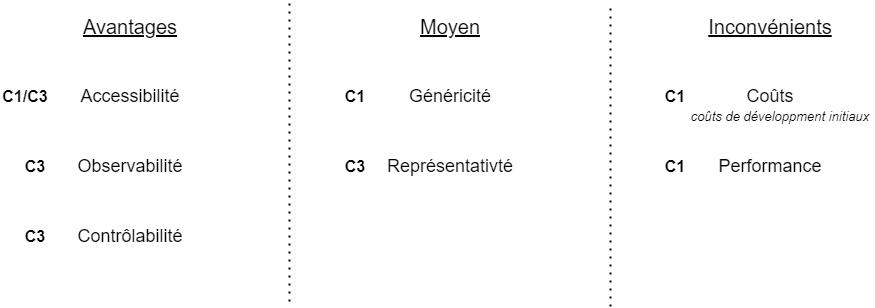
\includegraphics[scale=.56]{ch2-background/img/advantages-simu.drawio.png}
                  \caption{Comparaison des outils de simulation par rapport aux méthodes précédentes}
                  \label{fig:soa-tools-scheme-simu}
                \end{figure}
                
                On peut également opposer les simulateurs qui prennent en compte les fautes (comme Depend ou Celtic par exemple) et les implémentations qui s'appuient sur un simulateur existant et suivent alors le modèle \gls{swifi} en reproduisant l'effet d'une faute dans le modèle en question (tels que \gls{pafi}). 
                L'observabilité et le contrôle de la description des fautes est souvent bonne pour ce type de techniques puisque l'accès au système est plus facile sur un simulateur que sur le matériel et le simulateur peut accéder à des parties plus bas niveau du système que pour l'injection logicielle.
                
        \subsection{Méthodes formelles}
        \label{sec:soa-tools-formal}
            
            Les outils cités précédemment, à quelques exceptions près (comme Depend), comparent les exécutions fautées obtenues à une exécution de référence (\textit{golden run}). Pour chaque expérimentation ou simulation, les entrées du programme ou du système sont fixées ainsi que les fautes devant être injectées. Ces outils tentent de couvrir le maximum d'attaques en effectuant une série de tests avec différents paramètres pour les entrées et les fautes.
            
            Si différentes solutions ont été développées parmi ces outils basés sur les tests, comme réduire l'espace de faute \cite{Benso/TODAES98}, sélectionner un seul représentant pour une attaque \cite{Schmidt/Austrochip07} ou bien encore le développement de modèle plus haut niveau faisant abstraction de certains comportements, la couverture de ces outils est encore loin d'être parfaite. C'est pourquoi des solutions basées sur les méthodes formelles ont émergées afin d'obtenir une plus grande couverture des exécutions (des entrées et des fautes) ou bien de prouver des propriétés générales sur un programme ou un circuit, pour toutes fautes et pour toutes les entrées d'un modèle donné.
            
            \begin{figure}[hbt]\centering
              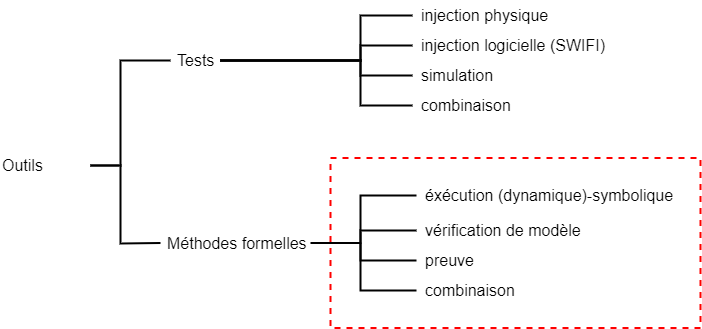
\includegraphics[scale=.45]{ch2-background/img/plan-soa-tools-formal.drawio.png}
              \caption{Outils basés sur les méthodes formelles}
              \label{fig:soa-tools-scheme-plan}
            \end{figure}
                
            La figure \ref{fig:soa-tools-scheme-plan} est un rappel du plan de la section \ref{sec:soa-tools} mettant en évidence les approches basées sur les méthodes formelles. 
            Ces outils basés peuvent parfois être rapprochés des techniques de simulation, dans le sens où le système n'est pas exécuté directement sur le matériel, mais analysé statiquement. C'est le cas pour l'exécution symbolique où le moteur d'exécution simule une exécution (ou plus exactement un ensemble d'exécutions) dans un modèle donné.
            De la même manière, certaines approches se rapprochent des méthodes de types \gls{swifi}, lorsque l'effet des fautes est mis en place dans le programme ou sa représentation, afin d'être fournies à un outil d'analyse formelle n'ayant pas de représentation pour les fautes \cite{Potet/ICST14, Le/DATE18}. 
            Les analyses formelles peuvent être appliquées à différents niveaux de représentation, en allant du niveau source aux représentations bas niveau comme le \gls{rtl} ou la spécification du circuit par exemple.             
            
            \paragraph{} 
            En 2007, Larsson et al. \cite{Larsson/VERIFY07} proposent une méthode appelée \textit{symbolic fault injection}. Ils présentent un outil d'analyse dans le cadre de la tolérance au fautes d'un programme source en Java et qui se base sur l'analyse formelle et l'exécution symbolique.
            Une instruction spécifique \texttt{inject(location);} est utilisée afin de spécifier que la zone mémoire \texttt{location} (variable, attribut etc.) peut être fautée. Leur implémentation utilise un modèle de bit flip sur les données et repose sur l'outil Key \cite{Ahrendt/Springer05}, une plateforme d'analyse formelle pour Java qui propose des fonctionnalités pour la vérification statique étendue, l'exécution symbolique, la vérification déductive et la spécification formelle.
            Des règles spécifiques ont été ajoutées dans Key pour simuler l'effet d'une faute dans l'état symbolique du programme.
            L'outil n'est cependant pas totalement automatique puisque l'utilisateur est sollicité pour spécifier les invariants de boucles par exemple.
            
            \textit{SymplFIED} \cite{Pattabiraman/DSN08}, est un outil d'évaluation reposant sur l'exécution symbolique et le model checking \cite{Pattabiraman/TC12}.
            L'outil prend en entrée un modèle de faute et un programme en assembleur qu'il transforme en un langage assembleur générique de type \gls{risc}.
            Cette représentation est implémentée avec le système Maude \cite{Clavel/ENTCS96, clavel2002maude} qui est un outil permettant la vérification de propriété sur un modèle et qui se base sur la \textit{rewritting logic}.
            SymplFIED supporte les fautes transitoires de un ou plusieurs bits dans le décodeur d'instruction, l'unité de calcul, les bus d'adresses et de données ou encore le fetch d'instruction, en faute unique.
            L'outil définit une procédure de modélisation de chaque type de faute sur le modèle machine dans Maude ainsi que des règles de propagation des erreurs entre les différents modules modélisés. Une erreur est représentée par un symbole \texttt{err} qui est propagé au fur et à mesure de l'exécution symbolique du programme.
            En plus de cela, l'outil vise à énumérer les cas d'erreurs qui ne sont pas détectées par des \textit{détecteurs}.
            La modélisation dans Maude fait quelques hypothèses comme l'absence d'erreur dans les détecteurs ou le fait que tout accès à une mémoire non initialisée donnera lieu à une exception et certaines opérations comme la multiplication ne sont pas exécutées symboliquement \cite{Pattabiraman/TC12}. 
            
            \textit{Lazart} \cite{Potet/ICST14} est un outil d'analyse de robustesse de programme sur la plateforme \gls{llvm} qui repose sur l'exécution symbolique effectuée par l'outil KLEE \cite{Cadar/OSDI08}. Lazart propose le modèle de l'inversion de test et chaque faute possible dans le programme est représentée par un booléen symbolique ce qui permet de générer les différents chemins d'attaque. 
            L'objectif d'attaque est défini à l'aide d'une propriété d'atteignabilité (par exemple le bloc d'authentification dans le programme \texttt{verify\_pin}) et les auteurs utilisent un algorithme de coloration de graphe pour réduire l'espace des fautes injectées (en ne considérant que les fautes sur les branches qui peuvent atteindre le bloc de base visé). 
            La dernière version (version 4) de Lazart est l'objet des chapitres \ref{chpt:lazart} et \ref{chpt:lazart-implem}. 
            
            En 2018, Le et al \cite{Le/DATE18} proposent aussi un outil reposant sur l'exécution symbolique au niveau \gls{llvm} utilisant KLEE.
            En ce sens, il ressemble à Lazart à la différence qu'il se concentre sur la tolérance aux fautes, c'est-à-dire avec un modèle bit-flip en simple faute qui vise le registre de calcul virtuel de \gls{llvm} ainsi que l'instruction \texttt{load}.
            Ils utilisent une version légèrement modifiée de KLEE dans la fonctionnalité permettant de démarrer l'exécution symbolique avec une \textit{graine} de manière à ne considérer que les chemins dans lesquelles l'injection d'une faute est possible.
            L'outil propose d'activer et désactiver l'injection localement ou globalement à l'aide de fonctions fournies dans une bibliothèque C qui est liée au programme à analyser.
            
            \begin{table}[h]
                {\tiny
                \begin{center}
                \setlength\tabcolsep{2.6pt}
                    \begin{tabular}{|l|l|l|l|l|l|l|l|l|l|}
                    \hline
                    Outil & Niveau & FA & Mode & Modèle & Fautes & Oracle & Technique & Mode & PAE \\ \hline
                    \begin{tabular}[c]{@{}l@{}}Larsson et al.\\ \cite{Larsson/VERIFY07}\end{tabular} & Source (Java) & Non & Interne & flip & 1 & \begin{tabular}[c]{@{}l@{}}propriété\\ logique\end{tabular} & \begin{tabular}[c]{@{}l@{}}MC + SE \\ (Key)\end{tabular} & Interne & Elevé \\ \hline
                    \begin{tabular}[c]{@{}l@{}}Symplified\\ \cite{Pattabiraman/DSN08}\end{tabular} & ASM (MISP) & Non & Interne & \begin{tabular}[c]{@{}l@{}}data (decoder,\\ bus, reg, mem)\end{tabular} & 1 & SDC & \begin{tabular}[c]{@{}l@{}}rewriting \\ logic + SE\\ (Maude)\end{tabular} & Interne & Elevé \\ \hline
                    \begin{tabular}[c]{@{}l@{}}Lazart\\ \cite{Potet/ICST14}\end{tabular} & LLVM & Oui & Externe & TI & X & logiciel & DSE (KLEE) & Externe & variable \\ \hline
                    \begin{tabular}[c]{@{}l@{}}Le et al.\\ \cite{Le/DATE18}\end{tabular} & LLVM & Non & Externe & \begin{tabular}[c]{@{}l@{}}bit-flip (reg.,\\ op.)\end{tabular} & 1 & logiciel & DSE (KLEE) & Externe & variable \\ \hline
                    \end{tabular}
                \end{center}
                }            
                \caption{Comparaison de quelques outils reposant sur l'analyse formelle
                \label{tbl:tools-formal}}
            \end{table}
            
            La table \ref{tbl:tools-formal} présente une table de comparaison d'outils basés sur l'analyse formelle.
            Les colonnes \textit{Niveau}, \textit{FA}, \textit{Modèle}, \textit{Faute} et \textit{Oracle} sont équivalentes à celles des tables précédentes.
            La colonne \textit{Mode} précise si l'outil utilise de façon externe un outil d'analyse formelle en instrumentant le code à la manière d'un outil \gls{swifi}.
            La colonne technique liste les méthodes formelles utilisées par l'outil.
            La colonne \textit{PAE} correspond au passage à l'échelle de l'outil.
            
            \begin{figure}[hbt]\centering
              
\includegraphics[scale=.43]{ch2-background/img/advantages-formal.drawio.png}
              \caption{Caractéristiques des méthodes formelles}
              \label{fig:soa-tools-scheme-formal}
            \end{figure}
            
            La figure \ref{fig:soa-tools-scheme-simu} présente les caractéristiques des outils basés sur les méthodes formelles.
            Les méthodes formelles ont un avantage en ce qui concerne la complétude des résultats, dépendant de la technique utilisée. 
            Ces approches étant appliquées à des niveaux variés d'abstraction, et donc de modèles de faute, la représentativité des
            résultats est très variable.
            La performance n'est pas réellement comparable par rapport aux outils basés sur les tests, puisque tous les chemins et toutes les combinaisons de fautes sont potentiellement explorés, mais certains outils souffrent d'un problème de passage à l'échelle, corrélé à la méthode formelle utilisée.
            L'accessibilité et l'automatisation ne sont pas toujours bons pour ces outils, demandant parfois une expertise de l'utilisateur dans la méthode formelle utilisée ou bien une intervention importante de la part de l'utilisateur \cite{Larsson/VERIFY07}.
    
        \subsection{Conclusion}
        \label{sec:soa-tools-conclusion}
            
            Des approches très variées ont été proposées pour l'évaluation de la robustesse dans le cadre de l'injection de fautes, comme l'ont montré les sections précédentes.
            
                \begin{table}[h]
                    {\small
                    \begin{center}
                    \setlength\tabcolsep{3.5pt}
                        \begin{tabular}{|l|c|c|c|c|}
                        \hline
                        Méthode & Mise-en-place & Représentativité & Reproductibilité & Observabilité  \\ \hline
                        Injection Physique & Très élevé & Très élevé & Faible - Elevé & Faible  \\ \hline
                        SWIFI & Faible & Faible - élevé & Moyen & Moyen  \\ \hline
                        Simulation & Faible elevé & Moyen - élevé & Elevé & Elevé - Très élevé  \\ \hline
                        Méthodes formelles & Faible - Elevé & Moyen - élevé & Moyen - elevé & Elevé - Très élevé  \\ \hline
                        \end{tabular}
                        
                        \vspace{0.2cm}
                        
                        \begin{tabular}{|l|c|c|c|c|c|}
                        \hline
                        Méthode & Contexte  & Complétude & Accessibilité & Généricité & Contexte \\ \hline
                        Inj Physique & Varié &Faible & Faible & Faible & Varié \\ \hline
                        Swifi & Varié & Faible & Moyen & Elevée & Varié \\ \hline
                        Simu & Varié & Faible & Moyen & Moyen - élevé & Varié \\ \hline
                        Formal & Limité & Elevé - Très élevé & Faible & Moyen - élevé & Limité \\ \hline
                        \end{tabular}
                    \end{center}
                    }           
                    \caption{Comparaison des méthodes d'analyse de robustesse contre les fautes \label{tbl:tools-conclusion}}
                \end{table}
            
            La table \ref{tbl:tools-conclusion} compare les caractéristiques de la section \ref{sec:soa-tools-carac} pour les différentes techniques d'analyse présentées dans les sections précédentes.
            Chaque valeur correspond à une pondération entre \textit{faible}, \textit{moyen}, \textit{élevé} et \textit{très élevé}, visant à préserver les rapports entre les classes de techniques d'analyse ainsi que les variations au sein d'une même classe.
            
            Les méthodes formelles ont un très net avantage en ce qui concerne la couverture des exécutions fautées, mais certaines techniques comme l'exécution symbolique souffrent de l'explosion combinatoire induite par les fautes pour le passage à l'échelle, en particulier dans un contexte multi-fautes.
            De plus, certaines propriétés et objectif d'attaque peuvent être difficiles à exprimer ou à analyser avec certaines approches formelles, notamment les propriétés basées sur la comparaisons de traces (canaux-auxiliaires) qui peuvent être plus simples à évaluer avec un golden run. 
            La simulation offre des avantages en termes de contrôlabilité.
            Les méthodes de type \gls{swifi} sont généralement les plus faciles à mettre en place.
            
            Certaines caractéristiques dépendent fortement des choix de conception et d'implémentation de l'outil. Si la contrôlabilité est difficile dans le cadre de l'injection physique, cette caractéristique dépend surtout de ce que l'outil met à disposition à l'utilisateur pour les autres classes d'outils, les outils simulant un système (que ce soit dans un simulateur ou par une modélisation formelle) étant aussi avantagés. 
            L'accessibilité est un bon exemple de caractéristique dépendant en grande partie de l'outil plus que de la méthode utilisée, qu'il s'agisse d'automatisation, de contrôlabilité ou d'expertise. 
            
            D'autres caractéristiques dépendent aussi fortement du niveau de représentation considéré par l'outil, qui peut être très variable au sein des outils d'une même méthode d'analyse. 
            Dans ce cas, le niveau de représentation de l'outil influe directement sur la représentativité, les modèles de faute supportés et la généricité de l'outil.
            
            L'outil Lazart, qui est l'objet du chapitre suivant, est un outil d'analyse formelle utilisant l'exécution dynamique-symbolique.
            Lazart utilise l'outil KLEE qui effectue une exécution dynamique-symbolique sur le code \gls{llvm} et peut ainsi être vu comme un simulateur utilisant un modèle mémoire et une représentation du système particuliers.
            Les fautes sont introduites par une mutation du programme fourni à KLEE, correspondant à ce qui existe dans le cadre des outils \gls{swifi} au niveau \gls{llvm}.
            
            Lazart vise à répondre à certaines problématiques tirées de cette section en ce qui concerne ce type d'outils reposant sur les méthodes formelle ainsi que l'émulation des fautes au niveau logiciel.
            
            \begin{itemize}
                \item \textit{Performance} et \textit{passage à l'échelle}: maîtriser le multi-fautes et l'explosion combinatoire engendrée.
                \item \textit{Représentativité}: limiter la perte de représentativité liée à la sur-couche de l'émulation des fautes.
                \item \textit{Accessibilité} et \textit{généricité}: limiter le niveau d'expertise requis pour l'utilisation de l'outil et laisser une contrôlabilité élevée à l'utilisateur.
            \end{itemize}
            
            Les contributions de Lazart visent ainsi à proposer des solutions pour ces problématiques:
            \begin{itemize}
                \item Support de l'inter-procédural et de la combinaison de modèles de faute ainsi qu'une description à grain fin des fautes par l'utilisateur (\textit{représentativité} et \textit{contrôlabilité}).
                \item Une \gls{api} Python facilitant la description des analyses et la présentation des résultats (\textit{accessibilité}).
                \item Une analyse plus fine des résultats produits.
            \end{itemize}
    
    

%\part{Lazart}
\chapter{Lazart}
\label{chpt:lazart}

\begin{tikzpicture}[remember picture,overlay]
\node[anchor=west,inner sep=0pt] at (current page text area.west|-0,3cm) {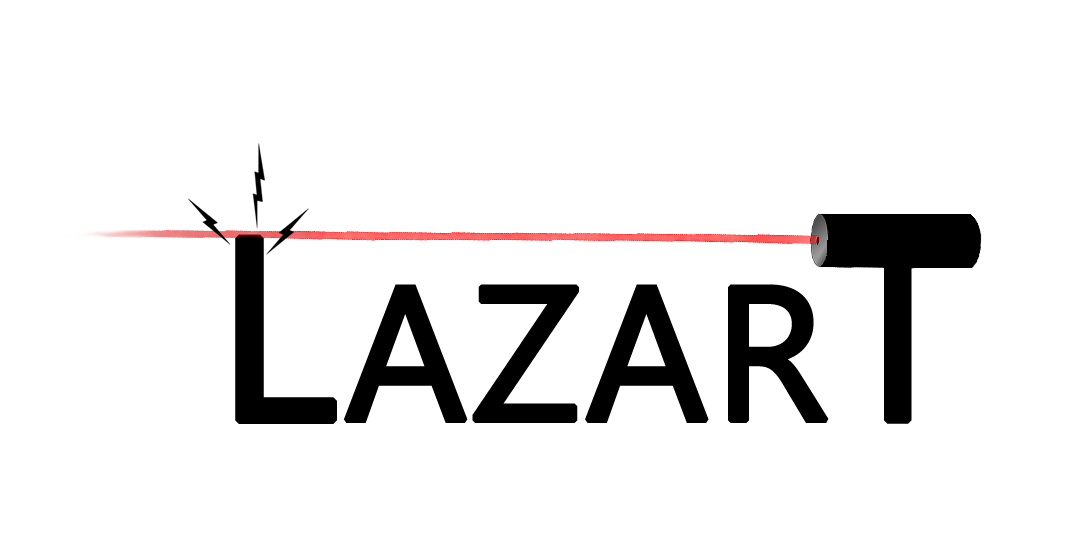
\includegraphics[height=3cm]{ch3-lazart/img/lazart-logo-red.png}};
\end{tikzpicture}

    Lazart \cite{Potet/ICST14} est un outil d'analyse de code haut niveau qui repose sur l'exécution symbolique et vise à évaluer la robustesse d'un programme dans le cadre de l'injection de fautes multiples. 
    Cet outil a été développé à Verimag depuis 2014 et a été étendu au cours de cette thèse. 
    Ce chapitre présente l'outil Lazart, dans sa version la plus récente, en décrivant son fonctionnement et son architecture du point de vue de l'utilisateur. 
    Il s'agira aussi de discuter de ses avantages et limitations par rapport aux outils présentés dans le chapitre précédant.
    Le chapitre \ref{chpt:lazart-implem} rentrera plus en détails dans l'implémentation de Lazart et discutera des choix qui ont été faits pour l'outil.
    
    La suite de ce chapitre est organisée comme suit.  
    La section \ref{sec:lazart-overview} présente le principe général de l'outil, la plateforme \gls{llvm} et l'exécution concolique sur lesquels Lazart s'appuie.
    La section \ref{sec:lazart-architecture} décrit l'architecture de l'outil et les différentes étapes d'une analyse.
    La section \ref{sec:lazart:descr} présente la façon dont l'utilisateur décrit les paramètres d'une analyse avec Lazart.
    La section \ref{sec:lazart-formal} s'intéresse à la représentation des traces dans Lazart ainsi qu'aux analyses de robustesse proposées par l'outil.
    La section \ref{lazart:metho} s'intéresse aux résultats fournis par l'outil, leur exploitation et à l'aspect méthodologique en présentant des évaluations réalisées avec Lazart.
    Finalement, la section \ref{sec:lazart:metho:concl} conclut ce chapitre.
    
    \setcounter{tocdepth}{2}
    \section*{Table des Matières}
    \localtableofcontents
    
    \section{Principe général et pré-requis}
    \label{sec:lazart-overview}
        
        Lazart est un outil d'analyse de code évaluant la robustesse d'un programme dans le cadre d'injection de fautes multiples. Il travaille au niveau de la représentation intermédiaire \gls{llvm-ir} et repose sur l'exécution concolique \cite{Baldoni/CSUR18} (pour concret-symbolique), qui combine l'exécution symbolique avec l'exécution concrète. 
        Lazart est destiné à être utilisé en amont du processus de développement pour aider le développeur à concevoir un programme sécurisé, ou en aval, en apportant une aide aux auditeurs pour en déterminer les vulnérabilités \cite{inter_cesti}. Il propose plusieurs analyses visant à évaluer la robustesse d'un programme dans le cadre de l'injection de fautes.
        L'outil est également destiné à l'évaluation de contre-mesures, cet aspect de l'outil sera présenté plus en détail dans les chapitre \ref{chpt:placement} et \ref{chpt:ccpo}.
        
        \begin{table}[h]
            \begin{center}
                \begin{tabular}{|l|l|l|l|l|l|}
                \hline
                \rowcolor[HTML]{C0C0C0} 
                Limite de faute                           & 0                         & 1                         & 2                         & 3                          & 4                          \\ \hline
                \cellcolor[HTML]{C0C0C0}Attaques       & \cellcolor[HTML]{9AFF99}0 & \cellcolor[HTML]{FFCCC9}1 & \cellcolor[HTML]{FFCCC9}5 & \cellcolor[HTML]{FFCCC9}10 & \cellcolor[HTML]{FFCCC9}11 \\ \hline
                \rowcolor[HTML]{FFCCC9} 
                \end{tabular}
                \caption{Résultat d'analyse d'attaque sur verify\_pin avec Lazart \label{tbl:vp-results}}
            \end{center}
        \end{table}
        
        L'analyse d'attaque permet de rechercher des chemins d'attaques dans un programme, en fonction d'un modèle d'attaquant (objectif d'attaque et modèle de faute). Cette analyse retourne la liste des chemins d'exécution fautés trouvés pour lesquels l'objectif d'attaque est atteint. La table \ref{tbl:vp-results} correspond aux résultats d'une analyse d'attaque pour le programme \texttt{verify\_pin} avec le modèle de l'inversion de test, une limite de fautes de quatre et comme objectif d'attaque $\phi_{auth}$, c'est-à-dire s'authentifier malgré un \gls{pin} faux. Chaque colonne indique le nombre de chemins d'attaques trouvés (deuxième ligne) pour un nombre de fautes fixé (première ligne).
     
        Lazart émule les fautes au niveau de la représentation intermédiaire \gls{llvm} et transmet le programme muté à l'exécution concolique de manière à explorer tous les chemins avec toutes les combinaisons de fautes possibles.
        La section \ref{sec:llvm} présente la plateforme \gls{llvm} et la représentation intermédiaire \gls{llvm-ir}, niveau auquel sont représentées les fautes.
        La section \ref{sec:se} présente le fonctionnement de l'exécution symbolique et la section \ref{sec:dse} décrit l'exécution concolique et les problématiques liées à ce mode de génération de traces. La section \ref{sec:klee} présente plus en détail l'outil KLEE et ses fonctionnalités et finalement, la section \ref{sec:dse-fi} s'intéresse à la façon dont les fautes sont simulées dans une implémentation pour le moteur d'exécution symbolique.
        
        \subsection{Low Level Virtual Machine (LLVM)}
        \label{sec:llvm}
        
            Lazart repose sur la plateforme \gls{llvm} \cite{llvm}, qui est un ensemble d'outils pour la conception de compilateurs, d'optimiseurs et d'outils d'analyse statique. \gls{llvm} est destiné à faciliter l'analyse et l'optimisation de programmes tout au long de la durée de vie d'un programme (\textit{lifelong program analysis and transformation}).            
            
            L'architecture \gls{llvm} (figure \ref{fig:llvm-arch}) s'organise autour de trois blocs majeurs: le front-end, la représentation intermédiaire et le back-end. 
            
            \begin{figure}[!h]\centering
                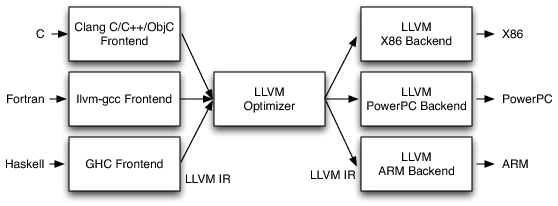
\includegraphics[scale=0.6]{ch3-lazart/img/LLVMCompiler.png}
                \caption{Architecture d'un compilateur en trois temps \cite{llvm/TAOSA}}  \label{fig:llvm-arch}
            \end{figure}
            
            Le \textit{front-end} compile le code source du programme en la \textit{représentation intermédiaire} qui est transformée en code binaire spécifique à l'architecture cible par le \textit{back-end}. Clang \cite{llvm} est certainement le front-end de compilateur le plus célèbre de \gls{llvm} et permet la compilation des langages C, C++, Objective-C et Objective-C++. \gls{llvm} supporte d'autres langages, tels que Rust, Swift, Haskell, D et Ada pour n'en citer que quelques uns, au travers d'autres front-end.
            
            Les analyses et optimisations sont effectuées sur la représentation intermédiaire \gls{llvm-ir}. La figure \ref{fig:llvm-arch} présente le cycle de vie d'un programme dans le cadre d'une compilation \gls{aot}, c'est-à-dire lorsque le processus d'optimisation et d'analyse a lieu en amont de l'exécution du programme. L'architecture de \gls{llvm} permet de simplifier l'optimisation inter-procédurale (\textit{link-time optimization}) en gardant la même représentation intermédiaire tout au long du cycle de vie. \gls{llvm} prend aussi en charge d'autres cycles de vie de programmes tels que:
            
            \begin{itemize}
                \item \textit{Install Time Optimisation}: le programme est optimisé au moment de son installation sur l'appareil. Il s'agit d'un type particulier de compilation \gls{aot} \footnote{C'est par exemple la méthode employée sur Android avec la machine virtuelle Dalvik (qui n'est pas basée sur \gls{llvm}).} qui permet d'avoir des informations exactes sur l'architecture et la machine cible.
                \item \gls{jit} optimisation : le programme est compilé et optimisé pendant son exécution. Le \gls{jit} est très largement utilisé pour les langages basés sur une machine virtuelle (Java, C\# par exemple).
                \item \textit{Idle Time Optimisation}: le programme peut-être optimisé entre les exécutions. 
            \end{itemize}            
            
            \paragraph{}
            La représentation intermédiaire de \gls{llvm} est ainsi manipulée par des passes d'analyse et d'optimisation tout au long de la durée de vie du programme. \gls{llvm-ir} est un langage correspondant à une abstraction des langages assembleur. Sa forme binaire (utilisée en mémoire pendant les opérations ou stockée sous la forme de fichier) peut être transformée en équivalent textuel (et inversement). Le listing \ref{lst:llvm} présente un exemple de code \texttt{Hello world} en \gls{llvm-ir} sous forme textuelle. 
        
\begin{center}
\lstset{language=C,style=codeC} 
\begin{lstlisting}[caption=Programme \textit{Hello World!} en IR LLVM (LLVM-9), label=lst:llvm]
@.str = private unnamed_addr constant [14 x i8] c"Hello world !\00", align 1

define dso_local i32 @main(i32 %0, i8** %1) {
  %3 = alloca i32, align 4
  %4 = alloca i32, align 4
  %5 = alloca i8**, align 8
  store i32 0, i32* %3, align 4
  store i32 %0, i32* %4, align 4
  store i8** %1, i8*** %5, align 8
  %6 = call i32 (i8*, ...) @printf(i8* getelementptr inbounds ([14 x i8], [14 x i8]* @.str, i64 0, i64 0))
  ret i32 0
}

declare dso_local i32 @printf(i8*, ...)
\end{lstlisting}
\end{center}

            \gls{llvm-ir} rend explicite le flot de contrôle et de données. Toute instruction appartient à un bloc de base et tout bloc de base appartient à une fonction. Le langage suit la forme \gls{ssa} \cite{ssa} \footnote{L'instruction \texttt{phi} correspondant à la forme standard (non-gated, c'est-à-dire que l'assignation conditionnelle n'est évaluée qu'à partir d'une variable) de la fonction $\phi$ de \gls{ssa}.} 
            qui impose que chaque variable soit assignée avant toute utilisation et que chaque variable soit assignée exactement une fois. \gls{llvm-ir} utilise un nombre infini de registres typés, identifiés par les $\%XX$ dans le programme d'exemple.
            Les conventions d'appels de fonctions sont abstraites à l'aide des instructions \texttt{ret} et \texttt{call}.
            
            Le langage utilise un jeu d'instructions comparable à \gls{risc} et est fortement typé. Toutes les conversions sont explicites, à l'aide notamment des instructions de conversion (\texttt{cast}, \texttt{trunc}, \texttt{zext} ...) et de l'instruction \texttt{getelementptr} qui permet d'abstraire les opérations d'arithmétique de pointeur tout en préservant le typage (c'est-à-dire que \texttt{getelementptr} effectue les calculs appropriés au type sous-jacent des opérandes). La ligne 10 du programme \ref{lst:llvm}  correspond à l'appel de la fonction C standard \texttt{printf} et l'accès à la chaîne de caractère globale \texttt{@.str} utilise l'instruction \texttt{getelementptr} \footnote{le mot clef \texttt{inbound} est utilisé (ligne 10) pour apporter des garanties sur l'accès à la mémoire pour les phases d'analyse.}.
            
            Les instructions \gls{llvm-ir} peuvent être utilisées de façon générique pour chaque type de donnée de base et existent en plusieurs versions. Par exemple, l'instruction arithmétique \texttt{add} est la même pour les différents types entiers ou flottant et supporte différentes opérandes (par exemple deux registres \texttt{add i16 \%var1, \%var2} ou bien avec une valeur immédiate \texttt{add i64 \%var, i64 10}).            
            
            L'allocation de mémoire fait la distinction entre la pile et le tas. Dans l'exemple \textit{Hello world} ci-dessus, une instruction \texttt{alloca} est utilisée pour allouer un espace mémoire sur la pile pour chaque argument et variable locale de la fonction \texttt{main} (\texttt{\%3}, \texttt{\%4} et \texttt{\%5}). L'allocation sur le tas est effectuée avec l'appel des primitives (par exemple \texttt{malloc} et \texttt{free}). La lecture et l'écriture en mémoire sont faites respectivement avec les instructions \texttt{load} et \texttt{store}. Dans l'exemple \ref{lst:llvm}, chaque opération précise l'alignement des données avec le mot clef \texttt{align}.
            
            La plateforme \gls{llvm} est largement utilisée dans le monde de la recherche et de l'industrie et la page \gls{llvm} \cite{llvm/pub} recense plus de 250 publications liées à la plateforme. Le projet \gls{llvm} sur Github \cite{llvm/github} compte plus de 4000 forks et 2000 contributeurs.  
     
        \subsection{Principe de l'exécution symbolique}
        \label{sec:se}
            
            L'exécution symbolique est une technique d'analyse de programme qui a été théorisée dans les années 70 \cite{Boyer/ACM75, King/ACM76, Clarke/TSE76} et qui vise à générer des entrées de tests pour couvrir chaque partie d'un programme. Le principe consiste à parcourir le programme en utilisant des \textit{variables symboliques} plutôt que des valeurs concrètes pour les entrées, et de résoudre la formule logique associée à chaque chemin d'exécution. 
            L'exécution \textit{dynamique-symbolique} regroupe un ensemble de techniques se basant sur une combinaison d'une exécution symbolique et d'exécution(s) concrète(s) dans le but d'adresser certaines problématiques liées à l'exécution symbolique (section \ref{sec:dse}).
            
            Pour la fonction \texttt{exemple} en Figure \ref{lst:dse-example}, un chemin d'exécution possible consiste à passer dans la branche \textit{then} de la première condition et atteindre l'assertion dans la branche \texttt{else} ligne 9. Un ensemble d'entrées possible pour arriver à cet état est $\{x = 1, y = 3\}$. On peut alors chercher s'il existe un ensemble d'entrées invalidant l'assertion, comme par exemple $\{x = 0, y = 3\}$. L'objectif d'un outil d'exécution symbolique est d'obtenir une couverture maximale des chemins du programme et de fournir des valeurs concrètes pour les entrées permettant d'exécuter chaque chemin.
   
            \begin{center}
            \lstset{language=C,style=codeC}    
            \begin{lstlisting}[caption=La fonction exemple, label=lst:dse-example]
void exemple(int x, int y) { 
    if (x + y > 2) {          
        z = 2*x + y;              
        if (z == 20) {       
            x = y;        
            print(x);          
        }
        else {         
            y *= 2;      
            assert(x != 0);
        }
    }
    else {                  
        foo();             
    }
}
            \end{lstlisting}
            \end{center}    
                
            Le moteur d'exécution symbolique maintient un \textit{état symbolique} et un \textit{prédicat de chemin}.
            L'\textit{état symbolique} $\sigma$ associe aux variables une expression symbolique qui est mise à jour à chaque fois qu'une affectation est rencontrée. Pour une affectation $var = expr$, $\sigma$ est mis à jour en associant $var$ à $\sigma(expr)$. La figure \ref{lst:dse-example-sigma} présente le code de la fonction \textit{exemple} avec l'évolution de l'état symbolique à chaque assignation dans le programme.
            
            \begin{center}
            \lstset{basicstyle=\large}
            \lstset{language=C,style=codeC}    
            \begin{lstlisting}[caption=Etats symboliques pour la fonction exemple, escapeinside={(*}{*)}, label=lst:dse-example-sigma]
void exemple(int x, int y) {    (* {\color{red} $\sigma \: = \: \{ \: x \: \to x_0, \: y \: \to \: y_0  \: \} $}*)
    if (x + y > 2) {        
        z = 2*x + y;            (* {\color{red} $\sigma \: = \: \{ \: z \: \to \: 2*x_0 \: + \: y_0, \: x \: \to x_0, \: y \: \to \: y_0 \: \} $}*)
        if (z == 20) {       
            x = z + 3;          (* {\color{red} $\sigma \: = \: \{ \: z \: \to \: 2*x_0 \: + \: y_0, \: x \: \to 2*x_0 \: + \: y_0 + \: 3, \: y \: \to \: y_0 \: \} $}*)
            print(x);           
        }
        else {
            y *= 2;             (* {\color{red} $\sigma \: = \: \{ \: z \: \to \: 2*x_0 \: + \: y_0, \: x \: \to x_0, \: y \: \to \: 2 * y_0 \: \} $}*)
            assert(x != 0);
        }
    }
    else {
        foo();      
    }
}
            \end{lstlisting}
            \end{center}     
         
            Le \textit{prédicat de chemin} (\gls{pathc}) est une formule logique du premier ordre qui est mise à jour à chaque fois qu'un branchement conditionnel est rencontré.
            La fonction \textit{exemple} contient donc cinq prédicats de chemin, présentés dans le listing \ref{lst:dse-example-pc}, dont les valeurs sont:
            
            \begin{eqnarray}
                PC_0 & \equiv & true \\
                PC_1 & \equiv & x_0 + y_0 > 2 \\
                PC_2 & \equiv & x_0 + y_0 > 2 \wedge 2 * x_0 + y_0 = 20 \\
                PC_3 & \equiv & x_0 + y_0 > 2 \wedge 2 * x_0 + y_0 \ne 20 \\
                PC_4 & \equiv & x_0 + y_0 <= 2 
            \end{eqnarray}
            
            \begin{center}
            \lstset{basicstyle=\large}
            \lstset{language=C,style=codeC}    
            \begin{lstlisting}[caption=La fonction exemple, label=lst:dse-example-pc]
void exemple(int x, int y) {    // PC0
    if (x + y > 2) {            // PC1
        z = 2*x + y;              
        if (z == 20) {          // PC2
            x = y;        
            print(x);          
        }
        else {                  // PC3
            y *= 2;
            assert(x != 0);  
        }
    }
    else {                      // PC4   
        foo();            
    }
}
            \end{lstlisting}
            \end{center} 
            
            Lorsqu'un branchement $if( expr )$ est rencontré, le prédicat de chemin est mis à jour tel que $PC_{then} = PC \wedge \sigma(expr)$ pour la branche vraie, et $PC_{else} = PC \wedge \neg \sigma(expr)$ pour la branche fausse. S'il existe une solution qui satisfait $PC_{then}$, l'exécution symbolique clone l'état symbolique $\sigma$ et continue avec le prédicat de chemin $PC_{then}$ dans la branche \textit{then}, et respectivement pour la branche \textit{else}.
            
            \paragraph{}            
            La résolution des prédicats de chemins est automatisée avec des solveurs de contraintes. 
            Les solveurs particulièrement utilisés dans ce contexte sont les solveurs \gls{smt} \cite{DeMoura/ACM11, Barrett/HMC18} qui permettent de prouver la satisfaisabilité de certaines classes de formules logiques du premier ordre sans quantificateur. Le solveur de contraintes prend en entrée une formule logique et peut indiquer si elle est satisfaisable (en exhibant une valuation des variables correspondantes), si elle est non satisfaisable (il n'existe aucune solution), ou bien ne pas conclure dans le temps imparti (\textit{timeout}). 
            
            L'évolution des solveurs \gls{smt} au cours de ces dernières décennies a permis de rendre réaliste l'usage des techniques d'exécution symbolique. Parmi les principales théories supportées on trouve l'arithmétique linéaire ou non linéaire (sur entiers ou réels), les tableaux, les vecteurs de bits, etc. 
            
            \paragraph{}            
            \begin{sloppypar}   
            On peut s'intéresser à la correction et la complétude des prédicats de chemins \cite{Godefroid/PLDI11}.
            \end{sloppypar}   
            
            \begin{defi}
            \label{def:pc-sound}
                Un prédicat de chemin $PC_{\omega}$ est \textit{correct} si tout modèle satisfaisant $PC_{\omega}$ fournit des entrées pour une exécution du programme suivant le chemin $\omega$.
            \end{defi}
            
            \begin{defi}
            \label{def:pc-complete}
                Un prédicat de chemin $PC_{\omega}$ est \textit{complet} si toute entrée suivant le chemin $\omega$ est un modèle validant $PC_{\omega}$.
            \end{defi}
        
        \subsection{Exécution dynamique-symbolique (DSE)}
        \label{sec:dse}                
            
            L'exécution \textit{dynamique-symbolique} (\gls{dse}) consiste à combiner l'exécution symbolique avec l'exécution concrète. Cela permet de résoudre en partie certains des problèmes liés à l'exécution symbolique, potentiellement au prix d'une perte de correction et de complétude lorsqu'une partie de l'analyse est concrétisée.
                   
            \begin{sloppypar}  
            Les premières approches sont apparues dans les années 2000 avec notamment le \textit{test concolique} introduit dans l'outil \gls{dart} \cite{Godefroid/PLDI05}. \gls{dart} propose de maintenir un état concret parallèlement à l'état symbolique. Cette approche nécessite des entrées concrètes au démarrage de l'analyse, qui peuvent être générées aléatoirement ou fournies par l'utilisateur. L'état concret associe chaque variable du programme à une valeur et maintient le prédicat de chemin et l'état symbolique de manière à calculer à l'aide du solveur des valeurs concrètes pour chaque chemin. Cette concrétisation permet notamment d'exécuter des fonctions externes à l'aide de valeurs concrètes sans disposer de leur code.        
            \end{sloppypar}  
            
            EXE \cite{Cadar/ACM08} et son successeur KLEE \cite{Cadar/OSDI08} utilisent une approche similaire que les auteurs nomment \textit{execution-generated testing}, proposée initialement en 2005 \cite{Cadar/SPIN05}, qui maintient également un état concret. Si une opération n'implique que des valeurs concrètes, celle-ci est exécutée directement, sinon, l'opération est effectuée symboliquement. 
            
            L'exécution dynamique-symbolique est limitée par un certain nombre de problématiques: la résolution des prédicats de chemin, le nombre de chemins générés, la modélisation du système et l'utilisation de code non disponible (comme une bibliothèque externe). La suite de cette section s'intéresse à ces problématiques et présente certaines approches qui ont été développées pour les pallier.
            
            \subsubsection{Complexité des formules passées au solveurs}
                
                Les solveurs de contraintes sont sensibles au type d'application considéré. Ils peuvent être limités si les théories supportées ne permettent pas (dans un temps raisonnable) de résoudre le prédicat de chemin ou bien si le prédicat de chemin contient des formules qui sont par nature difficiles à résoudre (comme inverser une fonction de hachage cryptographique par exemple). 
                
                Certaines techniques permettent cependant d'atténuer ces difficultés du côté du moteur d'exécution symbolique. Les formules logiques transmises aux solveurs peuvent être simplifiées ou optimisées par différentes techniques: réutilisation des résultats de résolution de contraintes (\textit{incremental solving} \cite{Sen/SIGSOFT05}),
                suppression des contraintes non liées au test qu'on veut valider ou inverser (\textit{irrelevant constraint elimination} \cite{Cadar/OSDI08}), simplification des expressions logiques passées au solveur, comme des simplifications linéaires ou des remplacements par des expressions équivalentes (par exemple transformer une puissance de 2 en un décalage de bit). La \textit{constraint set simplification} \cite{Cadar/ACM13} vise à simplifier les expressions du prédicat de chemin au fur et à mesure de l'exécution lorsque des contraintes plus précises sont rencontrées (par exemple $x_0 < 4 \wedge x_0 = 1 \: \to \:  x_0 = 1$).
                
                Outre la simplification des contraintes, le moteur d'exécution symbolique peut réduire le nombre d'appels au solveur par plusieurs techniques.
                Tout d'abord, le moteur peut continuer l'exploration sur certains chemins tandis que des requêtes sont en attente pour d'autres chemins. C'est par exemple ce que fait EXE qui utilise un serveur responsable de traiter les requêtes demandée par les différentes instantes du moteur d'exploration.
                Certains outils, tels que KLEE et Binsec \cite{Djoudi/CTACAS15, Binsecgithub}, proposent d'utiliser plusieurs solveurs de contraintes. Ceux-ci peuvent être appelés en parallèle ou bien choisis à l'aide d'heuristiques.  
                Des formats standards de requête aux solveurs tels que SMT-LIB \cite{BarFT-SMTLIB} ont été développés pour faciliter l'interchangeabilité des solveurs.
                La réutilisation des contraintes peut être faite en utilisant un cache des contraintes déjà envoyées au solveur: par exemple le \textit{constraint caching} effectuant du hash consing sur les contraintes \cite{Cadar/ACM13}, ou bien le \textit{counter example caching scheme} de KLEE, qui part du principe qu'en général l'ajout de contraintes n'invalide pas les solutions déjà trouvées.
                L'approche décrite dans \cite{yang2012memoized}, appelée \textit{memoized symbolic execution}, encode les préfixes des chemins d'exécution afin de les réutiliser. 
                Green Framework \cite{visser2012green, jia2015enhancing} propose d'aller plus loin en proposant la réutilisation de contraintes entre des programmes et des analyses différentes.
                Dans les cas où les contraintes sont trop complexes pour le solveur, la concrétisation de certaines variables est une solution. Certaines concrétisation peuvent néanmoins faire perdre la complétude.
                
            \subsubsection{Explosion des chemins}
                
                L'exécution symbolique est aussi sensible à \textit{l'explosion des chemins} (\textit{path explosion}). Le nombre de chemins d'exécution d'un programme peut rapidement devenir grand, voir infini (lorsque le programme contient des boucles dépendantes des entrées - que ce soit des boucles directes telles que des \textit{for}/\textit{while}, ou par récursion). S'il n'est pas possible de borner statiquement le nombre d'itérations, alors l'analyse doit se restreindre à une couverture partielle des chemins d'exécution. 
                
                Pour pallier la problématique d'explosion des chemins, plusieurs heuristiques peuvent être mises en place en plus de borner le nombre d'itérations ou la profondeur d'une exécution \cite{Cadar/OSDI08, Goderfoid/NDSS08, schwartz2010all, jamrozik2013generating}. 
                Ces heuristiques visent généralement en priorité la couverture de code (que ce soit au niveau des instructions ou des branches). Celles-ci comptent notamment la sélection aléatoire de chemins \cite{Cadar/ACM13}, le choix du chemin se rapprochant le plus d'une instruction non couverte, la sélection du chemin le plus court (\textit{shortest distance symbolic execution (SDSE)} \cite{chipounov2012s2e}) ou la sélection des chemins couverts le moins de fois. Certaines stratégies peuvent combiner plusieurs heuristiques (comme \textit{cov new} de KLEE) ou utiliser d'autres techniques comme le fuzzing \cite{majumdar2007hybrid, stephens2016driller, yun2018qsym}.
                
                La combinaison avec d'autres méthodes d'analyse peut également aider dans la réduction du nombre de chemins à explorer. Certaines fonctions peuvent être analysées indépendamment, de manière à générer des pré-conditions et post-conditions sur les entrées et sorties afin d'être ensuite réutilisées lors de l'appel de ces fonctions \cite{Godefroid/PLDI11}.
                Triton \cite{salwanthesis} propose aussi une option pour ne rendre symbolique que les espaces mémoires associés à une valeur teintée, la teinte étant propagée pendant l'exécution à partir des teintes initiales spécifiées par l'utilisateur.

            \subsubsection{Modélisation de l'architecture}
            
                La modélisation de l'architecture cible est également un problème important dans le cadre de l'exécution concolique et de l'analyse statique plus généralement. 
                Un modèle plus précis permet des résultats plus représentatifs mais peut être plus coûteux (notamment à cause d'une plus grande complexité des formules logiques passées aux solveurs). 
                
                Concernant la mémoire, différentes approchent existent. Certains outils considèrent toutes les variables d'un programme comme symboliques par défaut, comme c'est le cas pour Angr \cite{Shoshitaishvili/SSP16} par exemple. 
                D'autres comme KLEE nécessitent que l'utilisateur spécifie quelles sont les variables à rendre symboliques.
                La gestion de KLEE utilise un modèle mémoire composé de \og blocs mémoires \fg{} qui sont des tableaux de vecteurs de bits mais toutes les adresses (pointeurs) sont concrètes \cite{cadar2020klee}. 
                \gls{dart} utilise une approche similaire et concrétise un pointeur en prenant en compte le cas nul et le cas d'un objet complet. 
                Binsec représente la mémoire comme un tableau symbolique \cite{Djoudi/CTACAS15}.
                
                La prise en compte d'un environnement d'exécution complet (appels systèmes, bibliothèques externes, réseau...) est aussi une difficulté importante pour l'analyse statique d'un programme.
                Une solution consiste à interagir avec un environnement réel en concrétisant les paramètres au moment de l'appel. Cette approche est utilisée par EXE, \gls{dart} et CUTE par exemple, mais celle-ci souffre de l'incomplétude de la concrétisation.
                L'interaction avec un environnement concret nécessite de prendre des précautions pour que les interactions d'une exploration de chemin n'aient pas un effet de bord sur un prochain chemin, pour cela des solutions basées sur la virtualisation ont été mises en place (par exemple S2E \cite{chipounov2012s2e} qui utilise QEMU).
                Une autre solution est de rendre symbolique tout retour d'un appel externe afin de prendre en compte tous les comportements, ce qui mène toutefois à une sur-approximation.
                KLEE propose une implémentation de la bibliothèque standard C (appelée $\mu$libc) et qui peut être exécutée concrètement ou symboliquement pendant l'exécution concolique. Klover \cite{li2011klover} supporte aussi des bibliothèques POSIX supplémentaires.
                Certaines approches nécessitent l'intervention de l'utilisateur pour décrire un modèle \cite{xiao2011precise}. 

        \subsection{KLEE}
        \label{sec:klee}
        
            KLEE \cite{Cadar/OSDI08} est l'outil d'exécution symbolique utilisé dans Lazart. C'est un outil \emph{open-source} \cite{Klee/github} basé sur llvm-ir. En plus des caractéristiques déjà évoquées dans les sections précédentes, KLEE propose le paramétrage des stratégies d'exploration des chemins, le choix des solveurs à utiliser et l'accès aux formules \gls{smt} générées. L'outil supporte les solveurs STP \cite{ganesh2007decision}, boolector \cite{brummayer2009boolector}, CVC4 \cite{BarrettCDHJKRT11}, Yices 2  \cite{dutertre2014yices}, Z3  \cite{DeMoura/ACM11} et meta SMT \cite{haedicke2011metasmt}, qui est un projet permettant de supporter plusieurs solveurs de façon générique. 
            
            KLEE a été utilisé pour analyser la bibliothèque COREUTILS \cite{Coreutils} (plus de 400k lignes de code) et a permis de trouver 56 bugs majeurs dont 3 qui étaient inconnus jusqu'alors \cite{Cadar/OSDI08}. 
            L'outil a fini second lors de la compétition TestComp 2019 \cite{cadar2020klee} avec 1226 points contre 1238 pour l'outil Verifuzz \cite{basak2019verifuzz}, en ayant presque aucun point dans la catégorie des nombres en virgule flottante puisque ceux-ci ne sont pas supportés par KLEE.
            
            L'outil est largement utilisé pour différents types d'analyse de code (test fonctionnel, recherche de vulnérabilités, tolérance aux fautes, etc.) et la page \cite{klee-ref} recense plus de 100 publications liées à l'outil.
            Un certain nombre de projets ont été proposés à partir de KLEE.
            Cloud9 \cite{bucur2011parallel} est un projet open-source qui permet d'effectuer de l'exécution symbolique parallélisée avec KLEE, ce qui peut fortement améliorer les performances.
            Klover \cite{li2011klover} est une extension de KLEE proposant un support complet du C++ et qui utilise un solveur spécialisé pour les chaînes de caractères. 
            KleeNet \cite{sasnauskas2010kleenet} est un outil basé sur KLEE visant la recherche de chemins d'erreur dans des systèmes distribués et les piles de protocoles réseaux.
               
            \begin{sloppypar}  
            Le listing \ref{lst:klee} présente un exemple utilisation de KLEE contenant une fonction \texttt{foo} effectuant un branchement et le code d'analyse dans la fonction \texttt{main}.
            La fonction \texttt{klee\_make\_symbolic} (lignes 11 et 12) est utilisée pour déclarer une variable comme symbolique, la fonction prend en paramètre un pointeur vers la zone mémoire à rendre symbolique, sa taille et un nom (utilisé pour l'affichage des résultats).
            La fonction \texttt{klee\_assume} permet de couper l'exploration des chemins qui ne valident pas le prédicat en argument. Dans l'exemple (ligne 16), l'exploration se restreint aux exécutions où le retour de \textit{foo} est strictement positif. Cela permet d'encoder la vérification d'un objectif d'attaque par exemple.
            \end{sloppypar}  
            
            \begin{minipage}{\linewidth}
            \lstset{basicstyle=\large}
            \lstset{language=C,style=codeC}    
            \begin{lstlisting}[caption=Exemple d'instrumentation du programme pour KLEE, label=lst:klee]
int foo(int a, int b)
{
    if(b == 0)
        return a;
    return a / b;
}

int main() {
    int a;
    int b;
    klee_make_symbolic(&a, sizeof(a), "a"); // (memory pointer, size, name)
    klee_make_symbolic(&b, sizeof(b), "b");
    
    int result = foo(a, b);
    
    klee_assume(result > 0); // attack objective.
}
            \end{lstlisting}
            \end{minipage}
                
            KLEE fournit un ensemble de cas de tests (sous la forme de fichiers .ktest) qui correspondent chacun à un représentant d'un prédicat de chemin. Chaque cas de test est aussi associé à un type de terminaison qui peut être notamment:
            \begin{itemize}
                \item Une erreur d'exécution: adresse invalide lors d'une écriture ou lecture mémoire (\textit{ptr}), arithmétiques (division par zéro (\textit{div}), dépassement d'entier (\textit{overflow})), pointeur invalide fournit à \texttt{free} (\textit{free}), violation d'une mémoire read-only (\textit{rom}).
                \item Des comportement spécifiques: arrondi implicite (\textit{trunc}), conversion implicite (\textit{conv}).
                \item Une sortie secondaire: appel à la fonction standard \texttt{abort} ou à \texttt{klee\_abort} (\textit{abort}), assertion invalide (\textit{assert}). 
                \item Une erreur utilisateur (\textit{user}): un assume faux (\texttt{klee\_assume}) ou une utilisation incorrecte de KLEE.
                \item Concrétisation forcée (\textit{model}): appel symbolique à une fonction externe ou allocation de mémoire de taille symbolique par exemple.
                \item Une terminaison normale (aucun \texttt{klee\_assume} n'est violé) (\textit{satisfy}). 
                \item Un timeout: le chemin n'a pas pu être exploré dans le temps imparti (\textit{timeout}). 
            \end{itemize}            
            
            KLEE propose par ailleurs une fonctionnalité de replay qui permet de rejouer une exécution à partir d'un ktest en utilisant les valeurs du représentant pour les variables symboliques. Cela permet d'observer les sorties de l'exécution de ce chemin (sortie console ou interaction avec des fichiers par exemple).
            
        \subsection{Exécution symbolique et injection de fautes}
        \label{sec:dse-fi}
        
            Comme dit au début de ce chapitre, Lazart se base sur l'exécution concolique et le parcours des chemins pour chercher des attaques en fautes multiples. Cette section explique comment les fautes sont émulées pour le moteur d'exécution concolique.
        
            Le déclenchement potentiel d'un point d'injection est représenté à l'aide d'une variable symbolique interprétée comme un booléen, comme présenté dans la figure \ref{fig:symbolic-ip-pc}. Lorsque l'exécution symbolique rencontre un point d'injection, l'exécution est divisée en un chemin non fauté et un chemin fauté. 
            La fonction \texttt{symbolic\_bool} correspond à la génération d'une variable symbolique booléenne et la condition ligne 2 induit une division des chemins.
            Soit $PC_0$ le prédicat de chemin précédant le point d'injection, alors le chemin sans faute a pour prédicat de chemin  $PC_{normal} \equiv PC_0 \; \wedge \; \neg inject$ et celui fauté  $PC_{inject} \equiv PC_0 \; \wedge \; inject$. 
            Dans cet exemple, les variables \textit{\_fault\_count} et \textit{\_fault\_limit} correspondent respectivement au nombre de fautes injectées dans l'exécution en cours et à la limite de fautes.
            C'est en cela que l'approche utilisée par Lazart s'apparente aux outils de type \gls{swifi}, présentés dans le chapitre \ref{chpt:background}.
    
            \begin{figure}[H]\centering
            \begin{multicols}{2}
\lstset{language=C,style=codeC, caption={Comportement nominal},label=lst:symbolic-ip-nominal, showlines=true}
\begin{lstlisting}
normal_behavior()






\end{lstlisting}  
\columnbreak

\lstset{language=C,style=codeC, caption={Comportement avec fautes},label=lst:symbolic-ip-fault}
\begin{lstlisting}[label=lst-symbool]
inject = symbolic_bool()
if inject and _fault_count <= 
        _fault_limit:
    _fault_count++
    faulted_behavior()
else:
    normal_behavior()
\end{lstlisting}  
            \end{multicols}
            \caption{Représentation des fautes en pseudo-code pour l'exécution symbolique \label{fig:symbolic-ip-pc}}
            \end{figure}
        
            Ainsi l'exécution symbolique effectue un parcours de l'arbre d'exécution en y incluant toutes les exécutions fautées possibles. Cette disjonction des cas intensifie le phénomène d'\textit{explosion des chemins}, tout particulièrement dans le cadre de fautes multiples.
            Les fautes peuvent aussi introduire des chemins qui ne terminent pas.
            
            Illustrons cette explosion de chemins avec l'exemple de la fonction \texttt{fib} présentée dans le listing \ref{lst:fib} et qui correspond à une implémentation récursive du calcul de la suite de Fibonacci. Dans une exécution non fautée, cette fonction est constituée d'un ensemble d'exécutions correspondant à l'appel récursif de la fonction \texttt{fib} dépendant de l'entier naturel n.
    
\begin{lstlisting}[caption=Fonction \texttt{fib}, label=lst:fib]
uint fib(uint n) {
    if (n <= 1)
        return n;
    return fib(n-1) + fib(n-2); // IP1 et IP2
}
\end{lstlisting}  

            Si on considère un modèle de faute permettant de remplacer le retour d'un appel à \texttt{fib} par \texttt{0}, le programme contient deux points d'injection à la ligne 4, c'est-à-dire \texttt{fib(n-1)} ($IP_1$) et \texttt{fib(n-2)} ($IP_2$). Cela implique qu'à chaque appel à la fonction \texttt{fib(n)} dans une exécution normale, le chemin d'exécution se divise en cinq: le chemin retournant $n$, le chemin retournant \texttt{fib(n-1) + fib(n-2)} et les trois chemins fautés avec le déclenchement des points d'injection $\{IP_1\}$, $\{IP_2\}$ et $\{IP_1, IP_2\}$.
            
            Pour une exécution avec une valeur d'entrée $n$ fixée, l'exécution non fautée produit un unique chemin dont le nombre de blocs de base traversés dépend de $n$. Pour une exécution fautée, il existe $5^n$ chemins, pour un nombre de fautes non borné. 
            L'explosion du nombre de chemins est donc renforcée par la combinatoire des fautes en particulier en fautes multiples (ce problème est lié à l'injection de fautes et n'est pas spécifique à l'exécution concolique).
            
            \paragraph{}
            
            Les définitions \ref{def:pc-sound} et \ref{def:pc-complete} présentées précédemment définissent la \textit{correction} et la \textit{complétude} d'un prédicat de chemin $PC_{\omega}$.
            Soit $\Omega^M$ l'ensemble des chemins d'exécution fautée pour un programme $P$ et un modèle de faute $M$. 
            Un chemin d'exécution fautée $\omega \in \Omega^M$ peut correspondre à une exécution nominale (sans-faute) ou une attaque (exécution avec au moins une faute).
            On note $\mathcal{E}^M$ l'ensemble des prédicats de chemins fautés produits par un moteur d'exécution symbolique fauté $\epsilon$, séparant l'exploration des chemins entre le cas fauté et le cas non fauté, à chaque fois qu'un point d'injection est rencontré.
            
            On peut alors s'intéresser à la \textit{correction} et la \textit{complétude} d'un prédicat de chemin fauté $PC^M_{\omega}$, qui fournit des entrées et des fautes menant à une exécution suivant le chemin d'exécution fauté $\omega$ (définitions \ref{def:pcf-sound} et \ref{def:pcf-complete}).
            Les définitions \ref{def:fi-sound} et \ref{def:fi-complete} s'intéressent respectivement à la \textit{correction} et la \textit{complétude} de l'énumération des prédicats de chemins fautés $\mathcal{E}^M$ par un moteur d'exécution symbolique fauté $\epsilon$.
            
            \begin{defi}
            \label{def:pcf-sound}
                Un prédicat de chemin fauté $PC^M_{\omega}$ est \textit{correct} si tout modèle satisfaisant $PC^M_{\omega}$ fournit des entrées et des fautes pour une exécution (fautée) suivant le chemin $\omega$.
            \end{defi}
            
            \begin{defi}
            \label{def:pcf-complete}
                Un prédicat de chemin fauté $PC^M_{\omega}$ est \textit{complet} si toute paire (entrées, fautes) suivant le chemin $\omega$ est un modèle satisfaisant $PC^M_{\omega}$.
            \end{defi}

            \begin{sloppypar}
            \begin{defi}
            \label{def:fi-sound}
                L'énumération des prédicats de chemins fautés $\mathcal{E}^M$ est \textit{correcte} ssi, $\forall PC^M_{\omega} \in \mathcal{E}^M$, $PC^M_{\omega}$ est \textit{correct}.
            \end{defi}
            \end{sloppypar}
            
            \begin{defi}
            \label{def:fi-complete}
                L'énumération des prédicats de chemins fautés $\mathcal{E}^M$ est \textit{complète} ssi:
                \begin{itemize}
                    \item $\forall PC^M_{\omega} \in \mathcal{E}^M$, $PC^M_{\omega}$ est \textit{complet}, \textbf{et},
                    \item pour tout chemin d'exécution fauté $\omega \in \Omega^M$, $\exists PC^M_{\omega} \in \mathcal{E}^M$ tel que $PC^M_{\omega}$ fournit des entrées et des fautes pour une exécution (fautée) suivant le chemin fauté $\omega$.
                \end{itemize}
            \end{defi}

            La complétude de l'énumération des prédicats de chemins fautés (définition \ref{def:fi-complete}) correspond donc à avoir un ensemble de prédicats complets et que tous les chemins d'exécutions fautées soient représentés par au moins un prédicat de chemin dans $\mathcal{E}^M$.
            Avec l'émulation des fautes comme décrit dans la figure \ref{fig:symbolic-ip-pc}, les fautes sont des entrées (booléen symbolique).
            Chaque cas de test (ktest) fourni par KLEE correspond ainsi à un prédicat de chemin fauté avec un modèle représentant qui fournit ainsi les entrées et les fautes d'une exécution.
                
    \section{Fonctionnement et architecture de Lazart}
    \label{sec:lazart-architecture}
    
        La figure \ref{fig:lazart-analysis-scheme} présente le processus d'une analyse avec Lazart, qui s'organise en 5 étapes principales:
        \begin{itemize}
            \item \textit{Étape 1 :} l'utilisateur fournit le code source du programme et le modèle d'attaquant, décrit dans un \textit{script d'analyse} en Python et par l'instrumentation du programme.
            \item \textit{Étape 2 :} le programme est compilé pour produire le bytecode \gls{llvm-ir}.
            \item \textit{Étape 3 :} le bytecode est muté pour y introduire le comportement des fautes.
            \item \textit{Étape 4 :} le bytecode \gls{llvm-ir} muté est donné au moteur d'exécution concolique KLEE qui génère un ensemble de cas de tests (traces).
            \item \textit{Étape 5 :} les différents traitements sont effectués à partir des traces générées par KLEE.
        \end{itemize}
        
        \begin{figure}[!ht]\centering
            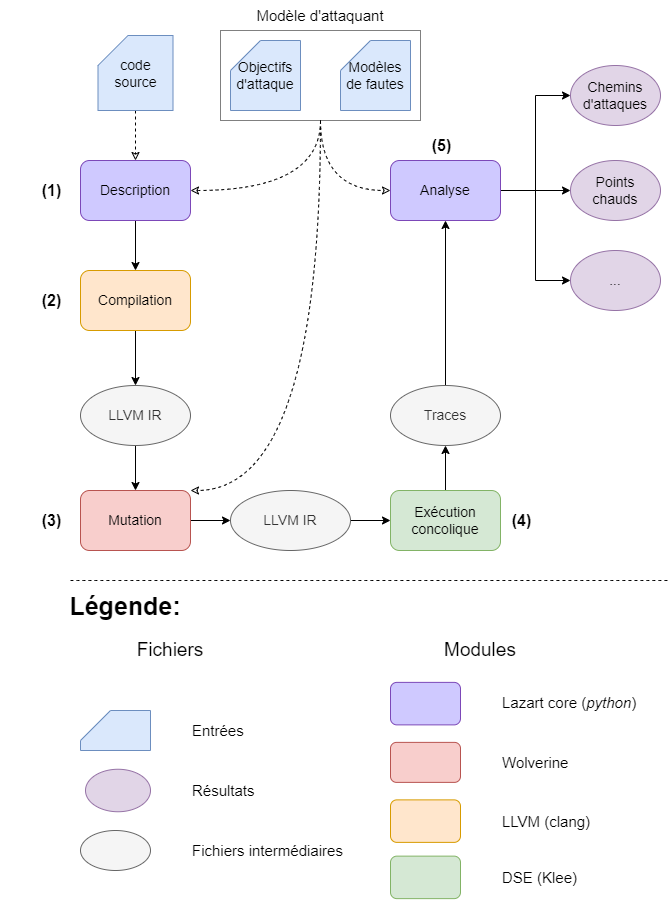
\includegraphics[scale=0.4]{ch3-lazart/img/lazart-workflow4_pack.drawio.png}
            \caption{Processus d'analyse avec Lazart}  \label{fig:lazart-analysis-scheme}
        \end{figure}
        
        Le fonctionnement indépendant des différentes étapes permet de reprendre une analyse en réutilisant les données intermédiaires des étapes précédentes, ceci afin de ne pas ré-exécuter certaines opérations coûteuses (comme l'exécution concolique). 
        Cette architecture modulaire permet aussi de simplifier l'intégration avec d'autres chaînes logicielles qui peuvent ainsi modifier une étape ou se placer entre les étapes du processus d'analyse. 
        
        Lazart est organisé en plusieurs modules: 
        \begin{itemize}
            \item \textit{Lazart Core}: une \gls{api} Python permettant la description et la manipulation des analyses, des traitements, des traces et des résultats.
            \item \textit{Wolverine}: l'outil permettant de muter un bytecode \gls{llvm} afin d'y introduire les potentielles fautes.
            \item \textit{Les outils externes} : dont notamment la chaîne de compilation de \gls{llvm} et l'outil d'exécution concolique KLEE.
        \end{itemize}
    
        Lazart Core permet à l'utilisateur de définir ses propres traitements à l'aide d'une \gls{api} en Python. Six traitements, appelés ici \og analyses \fg{}, sont proposés nativement dans Lazart:
        \begin{itemize}
            \item \textit{Recherche d'attaques}: recherche des chemins d'attaques.
            \item \textit{Analyse d'équivalence} : élimination des attaques \og équivalentes \fg{} (voir section \ref{sec:lazart-equivalence}).
            \item \textit{Analyse de redondance} : élimination des attaques \og redondantes \fg{} (voir section \ref{sec:lazart-redundancy}).
            \item \textit{Analyse de points chauds} : identification des points d'injection les plus sensibles (voir section \ref{sec:hotspots}).
            \item \textit{Analyses de placement de contre-mesures} : recherche des placements optimaux pour des contre-mesures \og locales \fg{} (décrites dans le chapitre \ref{chpt:placement}).
            \item \textit{Analyse d'optimisation de contre-mesures} : recherche des protections superflues ou redondantes dans une programme protégé  (décrite dans le chapitre \ref{chpt:ccpo}).
        \end{itemize}
            
        Lazart supporte trois modèles de faute: 
        \begin{itemize}
            \item \textit{L'inversion de test} (\gls{TI}): qui correspond à la sélection de la mauvaise branche lors d'un branchement conditionnel (instruction \texttt{br}).
            \item \textit{La mutation de données} (\gls{DL}): la donnée lue lors de l'exécution d'une instruction \texttt{load} est modifiée, la valeur injectée étant laissée au choix de l'utilisateur (valeur fixe ou valeur symbolique, éventuellement contrainte).
            \item \textit{Le saut arbitraire intra-procédural} (\gls{JMP}): la faute provoque un saut vers un point du programme (défini par l'utilisateur).
            \item[]
        \end{itemize}
        
        Ces trois modèles peuvent être combinés en multi-fautes, et permettent déjà d'exprimer un grand nombre de scénarios d'attaque.
        La suite de ce chapitre se concentre sur la description et l'utilisation des modèles de faute de Lazart pour l'utilisateur, le chapitre \ref{chpt:lazart-implem} reviendra plus en détail sur l'implémentation de ces modèles.
        
    \section{Description d'une analyse}
    \label{sec:lazart:descr}
    
        Cette section présente la description par l'utilisateur d'une analyse de recherche de chemin d'attaque avec Lazart.
        La section \ref{sec:lz:memcmps} présente la fonction \textit{memcmps} qui servira d'exemple.
        La section \ref{sec:lz:analysis-script} décrit le script d'analyse et les paramètres qui lui sont associés.
        La section \ref{sec:lazart-phi} s'intéresse à la description de l'objectif d'attaque et la section \ref{sec:lazart-am} à la description des modèles de faute.
        
        \subsection{La fonction \texttt{memcmps}}
        \label{sec:lz:memcmps}
        
            Les différentes étapes d'analyse  seront illustrées sur la fonction \texttt{memcmps} présentée dans le listing \ref{lst:example-memcmps}. 
            \texttt{memcmps} effectue une comparaison de deux tableaux d'octets en appelant plusieurs fois la fonction \texttt{memcmp} de la bibliothèque standard C de manière à se protéger contre des fautes. Si une faute sur la donnée ou une inversion de test fausse le résultat d'un appel à \texttt{memcmp}, la variable \texttt{result} ne contiendra ni \texttt{FALSE} ni \texttt{TRUE} et l'attaque sera donc détectée. 
            On considérera l'objectif d'attaque qui consiste à obtenir le retour \texttt{TRUE} malgré des entrées différentes, et la combinaison des modèles de faute d'inversion de test et de mutation de données arbitraire (non contrainte). 
        
\lstset{caption={Fonction \texttt{memcmps}},label=lst:example-memcmps}
\begin{lstlisting}    
// memcmps.h
typedef BOOL uint16_t;
#define TRUE    0x1234u
#define FALSE   0x5678u
#define MASK    0xABCDu

// memcmps.c
#include "memcmps.h"

BOOL memcmps(uint8_t* a, uint8_t* b, size_t len)
{
  BOOL result = FALSE;
  
  if (!memcmp(a, b, len)) {
    result ^= MASK;           // result = FALSE ^ MASK
    if (!memcmp(a, b, len)) {
      result ^= FALSE ^ TRUE; // result = MASK ^ TRUE
      if (!memcmp(a, b, len)) {
        result ^= MASK;       // result = TRUE
      }
    }
  }

  return result;
}
\end{lstlisting}
        
        \subsection{Script d'analyse et paramètres}
        \label{sec:lz:analysis-script}
            
            L'utilisateur décrit les paramètres et les traitements d'une analyse dans un \textit{script d'analyse} et en instrumentant le programme étudié.
            Le listing \ref{lst:vp-lazart-script} correspond au script d'analyse pour l'exemple \texttt{memcmps}.
            Ce script contient tout d'abord l'importation de Lazart (ligne 2). Les paramètres d'une analyse sont définis dans un objet de type \textit{Analysis}. Le constructeur (ligne 4) prend deux paramètres obligatoires: 
            \begin{itemize}
                \item les fichiers sources du programme: ligne 6, \texttt{memcmps.c} contenant la fonction à analyser ainsi que \texttt{main.c}, la fonction principale de l'analyse (voir section \ref{sec:lazart-phi}).
                \item le modèle d'attaquant, pour le moment représenté par la variable \texttt{attack\_model} (voir section \ref{sec:lazart-am}).
            \end{itemize}
            
\lstset{caption={Script d'analyse d'attaque pour l'exemple \texttt{memcmps}},language=python, label=lst:vp-lazart-script}
\begin{lstlisting}    
#!/usr/bin/python3
from lazart.lazart import *

a = Analysis(["memcmps.c", "main.c"], # Input files 
    attack_model, # Attack model
    flags=AnalysisFlag.AttacksAnalysis, # Analysis type
    compiler_args="-Wall",
    max_order=4,
    path="my_analysis")

execute(a)
\end{lstlisting}
            
            Un certain nombre de paramètres optionnels peuvent être spécifiés, la liste complète étant disponible dans l'annexe \ref{annexe:lz:analysis-args}.
            Dans l'exemple précédant, \texttt{flags} (ligne 6) indique les traitements qui seront effectués (ici une recherche d'attaques, \texttt{AttacksAnalysis}, la valeur par défaut).
            \texttt{compiler\_args} (ligne 7) indique les arguments supplémentaires pour l'étape de compilation et \texttt{max\_order} (ligne 8) correspond à la limite de fautes de l'analyse (par défaut 2). \texttt{path} (ligne 9) est le chemin du dossier d'analyse dans lequel les différents fichiers temporaires et les résultats seront stockés.
            
            La fonction \texttt{execute} lance les différentes étapes de l'analyse (conformément à la figure \ref{fig:lazart-analysis-scheme}) ainsi que la génération et l'affichage des résultats, en exécutant la séquence d'opérations\footnote{Dans le cadre d'une recherche de chemins d'attaques (\texttt{flag=AttacksAnalysis}) comme pour l'exemple \ref{lst:vp-lazart-script}.} indiquée dans le listing \ref{lst:vp-lazart-exec}. 
            
            \lstset{caption={Équivalent de la fonction \texttt{execute} pour une analyse d'attaque},language=python, label=lst:vp-lazart-exec}
\begin{lstlisting}    
compile_results(a) # Compilation.
run_results(a) # Mutation and DSE.
traces_results(a) # Gathering traces information from KLEE's ktests.
attacks_results(a) # Computing attacks analysis.
print_results(a) # Prints results of analysis.
generate_reports(a) # Generate analysis reports files.
\end{lstlisting}
            
            La suite de cette section explique comment l'utilisateur décrit l'objectif d'attaque et le modèle d'attaquant.

        \subsection{Description de l'objectif d'attaque}
        \label{sec:lazart-phi}
        
            L'objectif d'attaque est spécifié dans le programme à analyser.
            Le listing \ref{lst:vp-lazart-instr} présente le fichier principal de l'analyse \texttt{main.c}, instrumenté avec la spécification de l'objectif d'attaque. C'est cette fonction \texttt{main} qui sera le point d'entrée de l'exécution symbolique après l'étape de mutation.
            
            Les deux tableaux d'entrée \texttt{a1} et \texttt{a2} sont rendus symboliques à l'aide de la fonction \texttt{\_LZ\_\_SYM} (ligne 11 et 13) qui prend en paramètre le pointeur vers la zone mémoire à rendre symbolique et la taille de cette zone mémoire.
            L'objectif d'attaque est vérifié avec la macro \texttt{\_LZ\_\_ORACLE} qui limite la recherche aux d'exécutions qui valident le prédicat passé en paramètre.
            Elle permet ainsi de décrire la contrainte d'inégalité des entrées symboliques (ligne 19) et de vérifier que le retour de la fonction est \texttt{TRUE} (ligne 23).
            Les macros \texttt{\_LZ\_SYM} et \texttt{\_LZ\_ORACLE} sont implémentées à partir des directives de KLEE, respectivement \texttt{klee\_make\_symbolic} et \texttt{klee\_assume} (section \ref{sec:klee}).
             
\lstset{style=codeC, caption={Fonction principale de l'analyse},label=lst:vp-lazart-instr}
\begin{lstlisting}   
// main.c
#include "lazart.h"
#include "memcmps.h"

#define SIZE 4

int main()
{  
    // Inputs
    uint8_t a1[SIZE];
    _LZ__SYM(a1, SIZE); // Symbolic array
    uint8_t a2[SIZE];
    _LZ__SYM(a2, SIZE); // Symbolic array
    
    bool equals = true;
    for(size_t i = 0; i < SIZE; ++i)
        if(a1[i] != a2[i])
            equals = false;
    _LZ__ORACLE(!equal); // Consider only different inputs
    
    BOOL res = memcmps(a1, a2, SIZE); // Call studied function

    _LZ__ORACLE(res == TRUE); // Attack objective
}
\end{lstlisting}
        
        \subsection{Description des modèles de faute}
        \label{sec:lazart-am}
        
            Les modèles de faute peuvent être spécifiés de deux manières:
            \begin{itemize}
                \item dans le script d'analyse en Python (via l'argument \texttt{attack\_model}), permettant une granularité de l'ordre des fonctions ou des blocs de base.
                \item en instrumentant le code, ce qui permet un contrôle plus précis.
            \end{itemize}

            \begin{table}[h]
                \small
                \centering
\begin{tabular}{|l|cc|cc|}
\hline
\multicolumn{1}{|c|}{\multirow{2}{*}{Modèle}} & \multicolumn{2}{c|}{Description} & \multicolumn{2}{c|}{Granularité} \\ \cline{2-5} 
\multicolumn{1}{|c|}{} & \multicolumn{1}{c|}{Python} & Instr. & \multicolumn{1}{c|}{Python} & Instr. \\ \hline
Inversion de test (TI) & \multicolumn{1}{c|}{Oui} & Oui & \multicolumn{1}{c|}{\begin{tabular}[c]{@{}c@{}}Fonctions et blocs de\\ base\end{tabular}} & Branchements \\ \hline
\begin{tabular}[c]{@{}l@{}}Mutation de donnée (DL\\  - mutation de constantes\end{tabular} & \multicolumn{1}{c|}{\begin{tabular}[c]{@{}c@{}}Oui\\ Non\end{tabular}} & \begin{tabular}[c]{@{}c@{}}Oui\\ Oui\end{tabular} & \multicolumn{1}{c|}{\begin{tabular}[c]{@{}c@{}}Fonctions, blocs de base\\ et variables\end{tabular}} & Instructions \\ \hline
Saut arbitraire JMP) & \multicolumn{1}{c|}{Non} & Oui & \multicolumn{1}{c|}{N/ A} & Instructions \\ \hline
\end{tabular}
                \caption{Définition et granularité des modèles de faute}
                \label{tbl:lz:models-def}
                \end{table}
                
            La table \ref{tbl:lz:models-def} indique la granularité de chaque modèle de faute en fonction de la méthode de définition utilisée. La colonne \textit{Description} détermine si le modèle de faute peut être défini avec chaque méthode et la colonne \textit{Granularité} précise le niveau de granularité pour chaque méthode.
            La description en Python associe des modèles de faute à des portions de programme (fonction ou bloc de base), mais n'est disponible que pour l'inversion de test et la mutation de données.
            
            La suite de cette section explique comment ces modèles de faute sont décrits par l'utilisateur. 
        
            \subsubsection{Description du modèle d'attaquant en Python}
            \label{sec:lazart-am-py}
            
                La description du modèle d'attaquant en Python est faite en associant des modèles de faute à des fonctions ou des blocs de base du programme.
                Le listing \ref{lst:attack-model-python} présente un exemple de définition d'un modèle d'attaquant \texttt{am} composé de trois modèles de faute.
                L'annexe \ref{annexe:lz:param-analysis} décrit l'ensemble des paramètres disponibles pour chaque modèle de faute.
                
\lstset{caption={Exemple de modèle d'attaquant décrit en Python}, language=python, label=lst:attack-model-python}
\begin{lstlisting}  
model_ti = { "type": "test-inversion" }

model_breset = { 
    "type": "data-load",
    "all": 0 # All load are faulted to 0
    "exclude": ["i", "tmp"] # Except variables 'i' and 'tmp'.
}

model_gl = {
    "type": "data-load",
    "vars": {
        "my_global": "__sym__" # Arbitrary (unconstrained) value.
    }
}

am = {
    "functions": { # Associate models to functions.
        "__all__": [model_gl], # All functions
        "foo": [model_ti, model_breset]
    }
}
\end{lstlisting} 
                
                Dans l'exemple ci-dessus un modèle d'inversion de test (\texttt{model\_ti}) est appliqué sur la fonction \texttt{foo} avec le modèle de mutation de mise-à-zero (\texttt{model\_breset}). Le modèle \texttt{model\_gl} injecte une valeur arbitraire pour toute lecture de la variable \texttt{my\_global} (avec le mot clef \texttt{\_\_sym\_\_}). 
                Le champ \texttt{functions} permet l'application des modèles de faute sur des fonctions du programme (le champ \texttt{basic-blocks} est l'équivalent pour les blocs de base).
                
                Le listing \ref{lst:memcmps-am} présente le modèle d'attaquant pour l'exemple \texttt{memcmps} afin d'obtenir une combinaison de l'inversion de test et de la mutation de données. Une mutation en donnée arbitraire est appliquée sur les variables \texttt{result} et \texttt{len} et l'inversion de test est appliquée sur l'ensemble de la fonction.
                La ligne 14 est une version plus compacte de la définition de ce même modèle utilisant des fonctions utilitaires: \texttt{function\_list} associe un ensemble de modèles de faute à une liste de fonctions, et \texttt{ti\_model} et \texttt{data\_model} permettent de créer un modèle avec le champ \texttt{type} correspondant.
                
\lstset{caption={Modèle d'attaquant pour l'exemple \texttt{memcmps}}, label=lst:memcmps-am}
\begin{lstlisting}  
attack_model = {
    "functions" = {
        "memcmps" = [ {
                "type": "test-inversion"
            },
            { 
                "type": "data-load",
                "vars": { "result": "__sym__", "len":  "__sym__" }
            }
        ]
    }
}

attack_model = functions_list(["memcmps"], [ti_model(), data_model({ "vars": { "result": "__sym__", "len":  "__sym__" } })])
\end{lstlisting} 
                
            \subsubsection{Spécification du modèle de mutation de données}
            \label{sec:data-value}
        
                Le modèle de mutation de données de Lazart vise la généricité en laissant l'utilisateur spécifier la valeur qui sera injectée. Cette valeur peut être une constante, une valeur contrainte par un prédicat (encodé par une fonction définie par l'utilisateur dans le programme source) ou entièrement symbolique (non contrainte) pour le type donné. 
                Le listing \ref{lst:data-yaml-values} contient un exemple de description de la mutation de données pour chacun de ces cas.
    
\lstset{caption={Différentes spécifications de valeurs fautées en Python},label=lst:data-yaml-values}
\begin{lstlisting}  
{
    "type": "data-load",
    "vars": {
        "x": 0,               # Fixed value
        "y": "my_predicate",  # Constrained symbolic
        "z": "__sym__",       # Not-constrained symbolic
    }
}
\end{lstlisting}                 
                    
                Le listing \ref{lst:data-predicate-function} présente un exemple de deux prédicats \texttt{flip\_pred} et \texttt{bf\_pred} encodant respectivement le modèle d'inversion de tous les bits (\textit{flip}) et le modèle d'inversion d'un seul bit (\textit{bit-flip}), implémenté en langage C. Un prédicat prend en entrée la valeur originale (potentiellement symbolique) et la valeur injectée (toujours symbolique). 
               
\begin{lstlisting}[caption={Prédicat pour le modèle \textit{bit-flip}}, label=lst:data-predicate-function, language=C,style=codeC]
bool bf_pred(int value, int faulted)
{
    return hamming_distance(value, faulted) == 1; // on binary encoding.
}

bool flip_pred(int value, int faulted)
{
    return faulted == ~value;
}
\end{lstlisting}        
                    
                La table \ref{tbl:data-modele-mode} présente les types de mutation de données de Lazart permettant de représenter certains modèles de faute de la littérature.
                La première colonne indique le modèle de faute considéré et les colonnes suivantes indiquent si la méthode correspondante peut être utilisée (\textit{oui}) ou \textit{non}, \textit{possible} indiquant que la méthode peut représenter le modèle mais n'est pas la plus adaptée. 
                
                L'approche par \textit{prédicat} est la plus générique, pouvant s'appliquer dans tous les cas, la \textit{valeur fixe} et la valeur non-contrainte (\textit{symbolique}) étant réservées à des cas spécifiques.
                Le chapitre suivant (section \ref{sec:lazart-mfct-data}) s'intéresse aux considérations liées aux performances de l'analyse dans le choix de la fonction de mutation associé à chaque type de valeur fautée.
                
                \begin{table}[ht]
                \centering
                \small
                    \begin{tabular}{|l|c|c|c|}
                    \hline
                    Modèles de la littérature                                                     & \multicolumn{1}{l|}{Valeur fixe} & \multicolumn{1}{l|}{Symbolique} & \multicolumn{1}{l|}{Prédicat} \\ \hline
                    \begin{tabular}[c]{@{}l@{}}bit-set\\ bit-reset\end{tabular}   & possible                       & non                             & oui                           \\ \hline
                    bit-flip                                                      & non                              & non                             & oui                           \\ \hline
                    \begin{tabular}[c]{@{}l@{}}byte-set\\ byte-reset\end{tabular} & oui                              & non                             & oui                           \\ \hline
                    byte-flip                                                     & non                              & non                             & oui                           \\ \hline
                    \begin{tabular}[c]{@{}l@{}}set\\ reset\end{tabular}           & oui                              & non                             & possible                      \\ \hline
                    inversion                                                     & non                              & non                             & oui                           \\ \hline
                    valeur aléatoire                                              & non                              & oui                             & possible                      \\ \hline
                    valeur arbitraire                                             & non                              & oui                             & oui                           \\ \hline
                    \end{tabular}
                                \caption{Modèle de faute sur les données \label{tbl:data-modele-mode}}
                \end{table}
                    
            \subsubsection{Mutation par instrumentation}
            \label{sec:lazart-am-instr}
                
                L'instrumentation du programme est complémentaire à la description du modèle d'attaquant en Python. L'instrumentation peut être utilisée afin :
                \begin{itemize}
                    \item d'obtenir un contrôle plus fin sur l'application des modèles de faute.
                    \item de définir un point d'injection spécifique dans le programme.
                    \item de spécifier un modèle de faute non disponible via l'\gls{api} Python (saut arbitraire).
                \end{itemize}

                \begin{sloppypar}
                Le listing \ref{lst:instr-enable} présente une fonction \texttt{foo} contenant des macros de Lazart permettant le contrôle de l'activation de modèles. Les fonctions \texttt{\_LZ\_\_disable\_model}, et \texttt{\_LZ\_\_enable\_models} permettent respectivement de désactiver un modèle nommé (à l'aide du champ \texttt{name} d'un modèle de faute) et de réactiver tous les modèles.
                Ces fonctions doivent être placées en prenant en compte l'ordre dans lequel le compilateur va placer les blocs de base dans la représentation \gls{llvm-ir}\footnote{Cela dépend du compilateur et de sa version mais l'utilisateur peut inspecter le code \gls{llvm-ir} généré en cas d'ambiguïté.}.
                L'état d'activation des modèles n'est pas préservé entre les fonctions. 
                La fonction \texttt{\_LZ\_\_disable\_bb} permet ici de désactiver tous les modèles dans un bloc de base.
                \end{sloppypar}
                       
\lstset{style=codeC, caption={Activation et désactivation de modèles},label=lst:instr-enable}
\begin{lstlisting}     
int foo(int i, float f)
{
    _LZ__disable_model("fm:ti"); // Disable a named fault model.
    int ret = 0;
    if(a < 0)
    {
        _LZ__disable_bb(); // Disable all models in the current basic block.
        ret = a * f;
    }
    else
    {
        ret = bar(a * f);
    }
    _LZ__enable_models(); // Enable all disabled models.
    
    return ret;
}
\end{lstlisting}

                Le listing \ref{lst:instr-inplace} présente une fonction \texttt{bar} contenant des points d'injection définis manuellement. La fonction \texttt{\_LZ\_\_DATA\_i32} (ligne 6) permet de spécifier un point d'injection de mutation de données sur la constante \texttt{10} correspondant à la limite de boucle, le second paramètre est l'identifiant du point d'injection.
                Aux lignes 4 et 5, deux points d'injection de sauts d'instruction (\texttt{lend} et \texttt{end}) sont définis avec la macro \texttt{\_LZ\_\_JUMP}. La faute provoque un saut respectivement aux labels \texttt{loop\_end} (ligne 9) et \texttt{end} (ligne 12).
                        
\lstset{style=codeC, caption={Définition manuelle de points d'injection},label=lst:instr-inplace}
\begin{lstlisting}     
int bar(int a, int b)
{
    int total = 0;
    _LZ__JUMP(loop_end, "lend"); // (label, id)
    _LZ__JUMP(end, "end"); // (label, id)
    for(int i = 0; a < _LZ__DATA_i32(10, "loop_bound"); ++i) // (original, id)
    {
        total += a + b;
        loop_end:
    }
    
    end:
    return foo(total);
}
\end{lstlisting}               

    \section{Traces et traitements}
    \label{sec:lazart-formal}
     
        Les différents traitements de Lazart prennent en entrée un ensemble de traces d'exécution qui sont obtenues à partir des cas de tests de KLEE.
        Cette section présente la modélisation des traces au sein de Lazart (section \ref{sec:lz:traces}) et décrit les différentes analyses de robustesse de Lazart: \textit{l'analyse d'attaque} (section \ref{sec:lazart-aa}), \textit{l'analyse d'équivalence} (section \ref{sec:lazart-equivalence}), \textit{l'analyse de redondance} (section \ref{sec:lazart-redundancy}) et \textit{l'analyse de points chauds} (section \ref{sec:hotspots}).

        \subsection{Représentation des traces dans Lazart}
         \label{sec:lz:traces}

            Comme cela a été vu dans la section \ref{sec:dse-fi}, l'exécution concolique sur le mutant embarquant les fautes revient à une exploration de tous les chemins fautés\footnote{Dans le cas idéal, c'est-à-dire dans le cas où l'exécution concolique est complète. Les chemins fautés dépassant la limite de fautes fixée par l'utilisateur ne sont pas explorés.}. 
            Chaque cas de test généré par KLEE peut être vu comme une trace d'exécution représentant un ensemble d'exécutions qui suivent le même chemin et comprennent les mêmes déclenchements de fautes.
            Les valeurs concrètes (pour les entrées et les fautes) d'un cas de test permettent d'obtenir un représentant de cet ensemble d'exécutions.
            
            \begin{figure}[t]\centering
              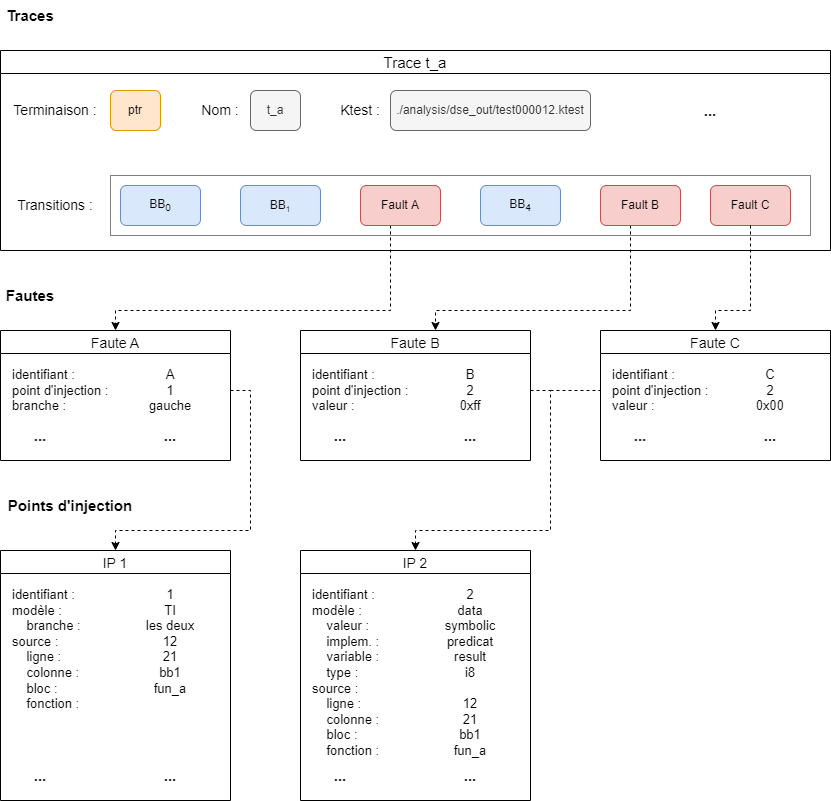
\includegraphics[scale=.43]{ch3-lazart/img/trace-model.drawio.png}
              \caption{Représentation d'une trace d'attaque dans Lazart \label{fig:lz-trace-model}}
            \end{figure}
            
            Ces traces d'exécution sont représentées dans Lazart par un type de \textit{terminaison}, et une liste ordonnée de \textit{transitions} pouvant être du type: 
            \begin{itemize}
                \item \textit{bloc de base}: entrée dans un bloc de base.
                \item \textit{faute}: un point d'injection a été déclenché.
            \end{itemize}
            
            \begin{defi}
                Soit $P$ un programme et $m$ un modèle de faute, on note $T(P, m)$ l'ensemble des traces d'exécution de $P$, ou plus simplement $T(P)$.
            \end{defi}
            
            Les transitions correspondant à l'entrée dans un bloc de base permettent de tracer le flot d'exécution. 
            Les transitions fautées sont paramétrées par le point d'injection déclenché (et donc le modèle de faute correspondant) et les paramètres de la faute. 
            Le type de terminaison d'une trace $t$, notée $Term(t)$, correspond aux terminaisons des cas de tests de KLEE\footnote{Pour rappel: \texttt{ptr}, \texttt{div}, \texttt{free}, \texttt{abord}, \texttt{assert}, \texttt{model}, \texttt{satisfy}, \texttt{timeout} etc.} (section \ref{sec:klee}) étendues avec la terminaison en contre-mesure (\texttt{detected}) et des cas d'erreurs supplémentaires spécifiques à Lazart (\texttt{lzerrs}).
            
            \begin{defi}
                Soit $t \in T(P)$, on note: 
                \begin{itemize}
                    \item $Tr(t)$ la liste ordonnée des transitions dans $t$.
                    \item $N(t)$ la liste ordonnée des transitions non fautées dans $t$.
                    \item $F(t)$ la liste ordonnée des transitions fautées dans $t$.
                \end{itemize}
            \end{defi}
        
            La figure \ref{fig:lz-trace-model} donne la représentation d'une trace d'exécution \texttt{t\_a} contenant la faute $A$ en inversion de test et les fautes $B$ et $C$ en mutation de données et deux points d'injection.
            
        \subsection{Analyse d'attaque}
        \label{sec:lazart-aa}
            
            L'analyse d'attaque correspond à la recherche de chemins d'attaques validant un objectif d'attaque $\phi$.
            
            \begin{defi}
                Une \textit{attaque} est une trace d'exécution comportant au moins une faute: $F(t) \neq \emptyset, t \; \in T(P)$.
            \end{defi}
            
            \begin{defi}
                Une \textit{attaque réussie}, pour un objectif d'attaque $\phi$, est une attaque validant l'objectif d'attaque: $F(t) \neq \emptyset \; \land t \vDash \phi, \; t \in T(P)$.
                
            \end{defi}
            
            La table \ref{tbl:memcmps-aa-results} donne le nombre de chemins d'attaque trouvés pour notre exemple avec une limite de fautes fixée à 4, et avec le modèle de faute combiné d'inversion de test et de mutation de données sur \texttt{result} et \texttt{i}. La taille des tableaux d'entrées est fixée à 4 et leurs valeurs sont symboliques (et contraintes d'être différentes sur au moins un octet
        
            \begin{table}[h]
                \caption{Chemins d'attaque trouvés avec \texttt{memcmps}}
                \label{tbl:memcmps-aa-results}
                \small
                \begin{center}
                    \begin{tabular}{l|llllll}
                    Fautes & 1F & 2F & 3F & 4F & 5F & Total \\
                    \hline
                    Attaques réussies & 0 & 4 & 8 & 20 & 28 & 60
                    \end{tabular}
                \end{center}
            \end{table}  
        
            \begin{figure}[!htp]\centering
                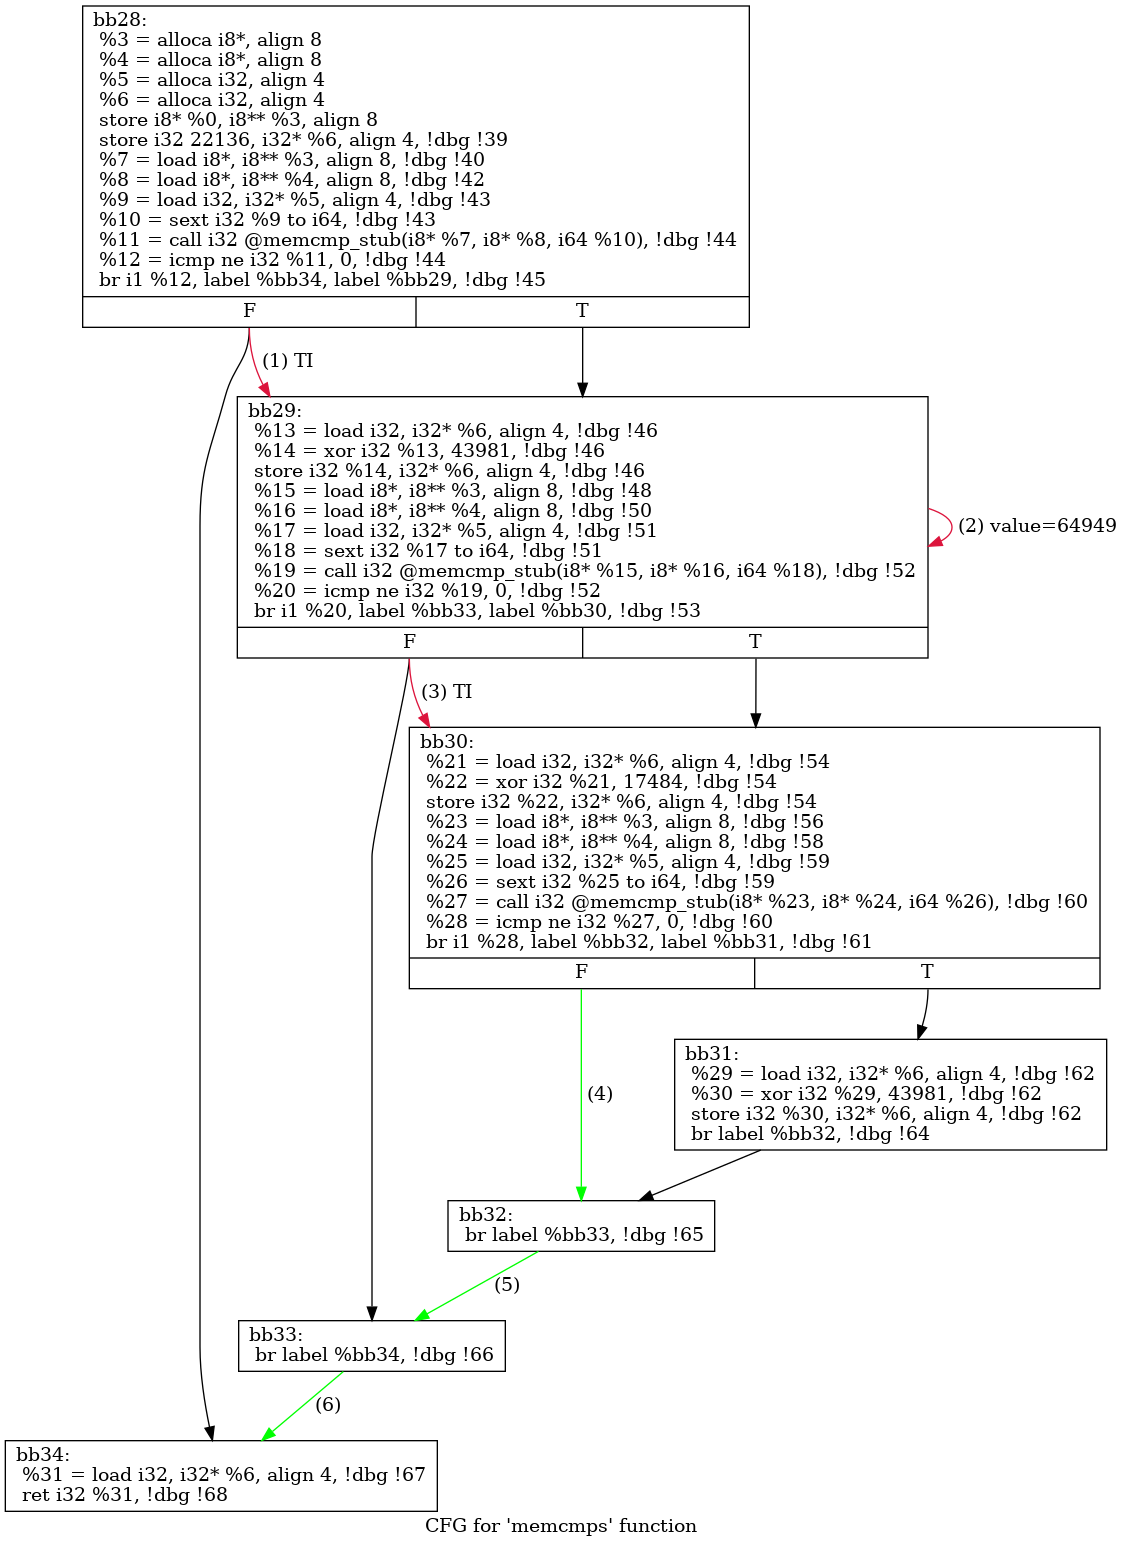
\includegraphics[scale=0.35]{ch3-lazart/img/cfg.memcmps.png}
                \caption{Graphe de faute de l'attaque en trois fautes sur \texttt{memcmps}}  \label{fig:memcmps-lazart-trace-graph}
            \end{figure}
        
            Le listing \ref{lst:memcmps-trace} présente une trace en trois fautes composée de deux inversions de test et une mutation de donnée.
            On y trouve en premier lieu le nombre de fautes dans la trace (\texttt{3}), son nom (\texttt{t15}) puis la liste ordonnée des transitions\footnote{Ici chaque faute indique dans l'ordre : l'identifiant du point d'injection concerné, le modèle de faute (ici \texttt{TI} ou \texttt{DL}), les informations spécifiques au modèle et finalement les informations sur la position du point d'injection dans le code source.}. Finalement le mot-clef \texttt{Satisfy} correspond au type de terminaison (ici l'objectif d'attaque a été validé).
            
            La figure \ref{fig:memcmps-lazart-trace-graph} correspond au graphe d'attaque généré par Lazart pour cette attaque. Le chemin suivi dans le graphe de flot de contrôle du programme étudié est indiqué en vert et les fautes sont indiquées en rouge.
            Cette attaque consiste à inverser le test du premier appel à \texttt{memcmp} (ligne 14\footnote{Voir code de \texttt{memcmps} dans le listing \ref{lst:example-memcmps}.}), puis injecter la valeur $FALSE \oplus MASK$ ($0x5678 \oplus 0xABCD = 64949$) dans la variable \textit{result} (ligne 15) et enfin inverser le test ligne 16. La ligne 17 est ainsi exécutée, on a $result = result \oplus FALSE \oplus TRUE \implies result = FALSE \oplus FALSE \oplus TRUE = TRUE$. Le dernier test n'est pas fauté et la ligne 19 n'est pas exécutée, la valeur $TRUE$ est donc retournée par la fonction.
                
    \lstset{caption={Attaque en trois fautes sur \texttt{memcmps}},language=python, label=lst:memcmps-trace}
\begin{lstlisting}   
(<3> t15: [BB(bb28), FAULT(0|TI|: bb28 => bb29 [l:27, bb:bb28]), BB(bb29), FAULT(1|DL|: ~ => 64949 [l:28, bb:bb29]), FAULT(2|TI|: bb29 => bb30 [l:29, bb:bb29]), BB(bb30), BB(bb32), BB(bb33), BB(bb34)]: Satisfy)
\end{lstlisting}               
                    
            \begin{sloppypar}
            Comme toutes les analyses de Lazart, l'analyse d'attaque prend l'argument \texttt{satisfies\_fct} correspondant à un prédicat déterminant si une trace valide l'objectif d'attaque ou non afin de laisser un contrôle fin à l'utilisateur. 
            Cela permet d'exprimer des objectifs d'attaque qui ne peuvent pas être décrits uniquement par l'instrumentation (par exemple des erreurs à l'exécution). 
            Le listing \ref{lst:s_fct} présente la définition d'un prédicat considérant comme une attaque les traces finissant en erreur arithmétique ou d'adresse, en plus des exécutions validant l'objectif d'attaque\footnote{Par défaut, seules les traces avec pour type de terminaison \textit{satisfy} sont prises en compte.}.
            La liste complète des paramètres des différentes analyses est donnée dans l'annexe \ref{annexe:lz:param-analysis}.                    
            \end{sloppypar}
                
    \lstset{caption={Filtrage des traces d'attaque en fonction de la terminaison},language=python, label=lst:s_fct}
\begin{lstlisting}    
Term = TerminationType # alias
attacks_analysis(satisfies_fct=lambda trace: trace.termination_is(Term.Satisfy, Term.Ptr, Term.Div, Term.Free))
\end{lstlisting}   
            
        \subsection{Équivalence des attaques et entrées symboliques}
        \label{sec:lazart-equivalence}
            
            Lazart propose les notions d'\textit{équivalence} et de \textit{redondance} (abordée en section \ref{sec:lazart-redundancy}) qui forment une relation d'ordre partiel entre les attaques permettant de présenter en priorité certaines attaques à l'utilisateur.
            Ces notions visent à aider à la protection et l'évaluation du code, en permettant de cibler les attaques jugées plus importantes.   
            
            Deux définitions d'équivalence sont proposées par Lazart nativement. Elles visent chacune à regrouper entre-elles des traces d'attaques selon des objectifs différents:
            \begin{itemize}
                \item[] \textbf{1)} \textit{Équivalence} (section \ref{sec:eq}): vise à pallier à une problématique relative à une division de certains chemins d'attaques, en raison du code implémentant la vérification de l'objectif d'attaque dans le cadre d'entrées symboliques.
                \item[] \textbf{2)} \textit{Faute-équivalence} (section \ref{sec:feq}): vise à regrouper des attaques qui ne diffèrent que par des variations légères et que l'on souhaite ne pas distinguer pour l'utilisateur.
            \end{itemize}
        
            \subsubsection{Distinguabilité et équivalence}
            \label{sec:eq}

                \begin{defi}[Équivalence]
                    \label{def:eq}
                    Une \textit{attaque} $a$ est dite \textbf{équivalente} (noté $\equiv$) à une attaque $a'$ si leur séquence de transitions sont égales (égalité syntaxique des séquences): \\
                    $a \; \equiv \; a' \;\;=_{def} \; Tr(a) = Tr(a')$ %\wedge Term(a) = Term(a')
                \end{defi}
            
                La notion d'équivalence des attaques (définition \ref{def:eq}) vise à regrouper les attaques qui suivent le même chemin, contiennent les mêmes fautes, mais ont des contraintes sur les entrées différentes.
                On définira la \textit{distinguabilité} d'un prédicat de chemin fauté au sein d'un ensemble $\omega^M$ (définition \ref{def:pcf-distinct}) et la \textit{distinguabilité} de l'énumération des prédicats de chemins fautés (définition \ref{def:fi-distinct}).  
            
                \begin{defi}
                \label{def:pcf-distinct}
                    Un prédicat de chemin fauté $PC^M_{\omega}$ est dit \textit{distinct} dans $\mathcal{E}^M$, si pour tout modèle $m$ satisfaisant $PC^M_{\omega}$, il \textit{n'existe pas} $PC' \in \mathcal{E}^M$ tel que $m \vDash PC'$.
                \end{defi}
                
                
                \begin{defi}
                \label{def:fi-distinct}
                    L'énumération des prédicats de chemins fautés (d'une exécution symbolique fautée $\epsilon$) est \textit{distincte} si tous les prédicats de chemins sont distincts.
                \end{defi}
                
                Il est possible que l'exécution concolique fautée ne soit pas \textit{distincte}, par exemple à cause du code encodant la vérification de l'objectif d'attaque qui divise certains chemins en plusieurs chemins non distincts (équivalents).
                Le programme présenté dans le listing \ref{lst:equiv} compte le nombre d'octets nuls dans un tableau de taille donnée. 
                Une exécution symbolique sur la fonction \texttt{null\_bytes} produit quatre chemins pour \texttt{size} fixé à 2:
                \begin{itemize}
                    \item Le chemin avec: $tab[0] = 0 \land tab[1] = 0 $.
                    \item Le chemin avec: $tab[0] \neq 0 \land tab[1] = 0 $.
                    \item Le chemin avec: $tab[0] = 0 \land tab[1] \neq 0 $.
                    \item Le chemin avec: $tab[0] \neq 0 \land tab[1] \neq 0 $.
                \end{itemize}
                
                Ces quatre chemins sont distincts (les séquences de transitions ne sont pas strictement équivalentes), chacun exécutant ou non l'incrémentation (ligne 5) à chacun des deux tours de boucle. 
                
\begin{center}
\lstset{language=C,style=codeC} 
\begin{lstlisting}[caption=Fonction \texttt{null\_bytes}, label=lst:equiv]
int null_bytes(uint8_t* tab, size_t size) {
    int total = 0;
    for(int i = 0; i < size; i++)
        if(tab[i] == 0)
            total++;
    return total;
}
\end{lstlisting}
\end{center}
                    
                Un objectif d'attaque consiste à retourner la mauvaise valeur en injectant des fautes \footnote{Silent Data Corruption (\gls{sdc}).}.
                Il est nécessaire d'encoder cette propriété dans le programme et pour cela, une méthode classique consiste à appeler la fonction étudiée sans injecter de faute et comparer les résultats, comme présenté dans le listing \ref{lst:equiv-oracle}. 
                Le tableau \texttt{tab} est rendu symbolique (ligne 3) et la valeur retournée (\texttt{ret}) est comparée à une version non fautée de la fonction à étudier (ici \texttt{null\_bytes\_safe} ligne 8).
                    
\begin{center}
\lstset{language=C,style=codeC} 
\begin{lstlisting}[caption=Point d'entrée de l'analyse pour \texttt{null\_bytes}, label=lst:equiv-oracle]
int main() {
    uint8_t tab[SIZE];
    _LZ__SYM(&tab, SIZE);
    
    int ret = null_bytes(tab, SIZE);
    
    // Verify attack objectives
    _LZ__ORACLE(ret != null_bytes_safe(tab, SIZE)); // Attacks division
}
\end{lstlisting}
\end{center}                    
                Pour chaque chemin atteignant le point de vérification de l'objectif d'attaque (ligne 8), la fonction \texttt{null\_bytes\_safe} est exécutée par le moteur d'exécution concolique.
                Dans le cas d'une exécution nominale, l'appel à \texttt{null\_bytes\_safe} produit exactement les mêmes contraintes pour chaque chemin que l'appel à \texttt{null\_bytes}, seuls quatre chemins sont donc générés, aucun ne validant l'objectif d'attaque.
                Dans le cadre d'une exécution fautée, l'appel à \texttt{null\_bytes\_safe} peut diviser certains chemins d'attaque, en ajoutant des contraintes différentes de celles de \texttt{null\_bytes} en raison des fautes.
                Si un chemin est divisé en plusieurs chemin qui valident l'objectif d'attaque, plusieurs ktests sont produits par KLEE alors qu'ils suivent le même chemin (dans la fonction étudiée \texttt{null\_bytes}, mais dont le chemin diffère dans \texttt{null\_bytes\_safe}) et contiennent les mêmes points d'injection de fautes.
    
                La table \ref{tbl:eq-results-prepost} compare les résultats obtenus pour les trois variantes de l'encodage de l'objectif d'attaque:
                \begin{itemize}
                    \item \textit{fix}: le tableau d'entrée est fixé à [1, 1].
                    \item \textit{sym-post}: le tableau d'entrée est symbolique et l'objectif d'attaque est vérifié à la fin.
                    \item \textit{sym-pre}: le tableau d'entrée est symbolique et l'objectif d'attaque est vérifié à la fin, mais la valeur attendue est pré-calculée avant l'appel de la fonction à analyser.
                \end{itemize}

                \begin{table}[h]
                    \caption{Résultats d'analyse d'équivalence sur les attaques réussies pour \texttt{null\_bytes}}
                    \label{tbl:eq-results-prepost}
                    \small
                    \begin{center}
                        \begin{tabular}{l|llllll}
                                 & Chemins Expl. & Traces & Attaques    & 1 faute & 2 fautes & Total \\
                                 \hline
                        \textit{fix}      & 14 & 11  & attaques    & 7       & 4        & 11    \\
                                 &    &     & classes eq. & 7       & 4        & 11    \\
                        \textit{sym-pre}  & 14 & 11  & attaques    & 7       & 4        & 11    \\
                                 &    &     & classes eq. & 7       & 4        & 11    \\
                        \textit{sym-post} & 19 & 16  & attaques    & 9       & 7        & 16    \\
                                 &    &     & classes eq. & 8       & 4        & 12  
                        \end{tabular}
                    \end{center}
                \end{table} 
            
                La colonne "Chemins Expl." indique le nombre de chemins explorés par KLEE, et "Traces" le nombre de traces générées par Lazart.
                Les colonnes suivantes indiquent le nombre d'attaques réussies trouvées (ligne "attaques") et le nombre de classes d'équivalence obtenues (ligne "classes eq.").
                On peut constater que l'analyse est \textit{distincte} en cas de pre-vérification dans cet exemple contrairement à la post vérification. 
                Les attaques obtenues après équivalence (lignes "classes eq.") sont bien égales entre les versions \textit{sym-pre} et \textit{sym-post}, à l'exception d'une classe d'équivalence supplémentaire qui n'est pas trouvée dans le cas \textit{sym-pre}. 
                Le pré-calcul est plus efficace puisque les contraintes sur les entrées sont exprimées avant l'appel de la fonction à étudier. Par conséquent, certains chemins peuvent être coupés directement pendant l'exécution symbolique fautée de \texttt{null\_bytes}.
                La version \textit{sym-pre} est aussi plus efficace, moins de chemins étant explorés.
                La version \textit{fix} est distincte mais est incomplète par rapport à l'utilisation d'entrées symboliques.
                L'utilisateur devrait dans le cas idéal préférer calculer au plus tôt les variables nécessaires pour vérifier l'objectif d'attaque (valeur attendues, contraintes des entrées...), même si cet exemple illustre le cas où un chemin supplémentaire est obtenu dans le cas de pre-vérification.
                
                En résumé, la notion d'équivalence (définition \ref{def:eq}) permet de regrouper les attaques qui ne varient que par leurs contraintes sur les entrées\footnote{Et potentiellement qui varient aussi au niveau du chemin dans l'encodage de l'objectif d'attaque.} de manière à ne présenter que les groupes d'équivalence à l'utilisateur.

            \subsubsection{Faute-équivalence}
            \label{sec:feq}
            
                La définition d'\textit{équivalence} impose la stricte égalité des transitions des attaques.
                La définition \textit{faute-équivalence} (définition \ref{def:feq}) se concentre sur l'égalité de la liste des transitions fautées uniquement.
                Cette définition ignore ainsi les variations de chemins (transitions non fautées) entre le déclenchement des fautes. 
                
                \begin{defi}[Faute-équivalence]
                    \label{def:feq}
                    Une \textit{attaque} $a$ est dite \textbf{faute-équivalente} (noté $\sim_f$) à une attaque $a'$ si leur séquence de transitions fautées sont égales (égalité syntaxique des séquences des fautes \footnote{Seuls les points d'injection sont comparés, pas les paramètres de fautes tels que la valeur d'une donnée injectée.}): \\
                    $a \; \sim_f \; a' \;\;=_{def} \; F(a) = F(a')$ 
                \end{defi}
            
                Cette définition vise à regrouper entre-elles des attaques qui ne diffèrent que par des variations de chemins liées aux entrées mais contiennent les mêmes fautes. Parmi ces différences qui sont captées par la \textit{faute-équivalence}:
                \begin{itemize}
                    \item des attaques qui diffèrent par un branchement n'ayant pas d'impact sur l'objectif d'attaque.
                    \item des attaques qui diffèrent par des fautes injectées à des itérations différentes dans une boucle.
                \end{itemize}
                
                La table \ref{tbl:aeq-results} compare les résultats obtenus pour \texttt{null\_bytes} avec les deux définitions de l'équivalence et donne les résultats obtenus pour l'inversion de test avec un objectif d'attaque visant à retourner un résultat incorrect (\gls{sdc}).
                La ligne \textit{attaques} correspond au total d'attaques réussies avant l'analyse d'\textit{équivalence}.
                La suivante correspond aux résultats d'équivalence et la troisième aux résultats de \textit{faute-équivalence}.

                \begin{table}[ht]
                    \caption{Comparaison des définitions de l'équivalence sur \texttt{null\_bytes}}
                    \label{tbl:aeq-results}
                    \small
                    \begin{center}
                        \begin{tabular}{l|llllll}
                        Fautes & 1F & 2F & 3F & Total \\
                        \hline
                        attaques & 13 & 5 & 0 & 18\\
                        classes d'équivalence & 11 & 4 & 0 &  15 \\
                          %- dont singletons & 10 & 3 & 0 & 13 \\
                        classes de faute-équivalence & 2 & 2 & 0 & 4\\
                          %- dont singletons & 0 & 0 & 0 & 0 \\
                        \end{tabular}
                    \end{center}
                \end{table} 
            
                Seules deux classes de faute-équivalence en une faute sont trouvées:
                \begin{itemize}
                    \item L'attaque consistant à inverser la condition d'entrée dans la boucle \texttt{for} (ligne 3). Cette attaque ne fonctionne que si le tableau d'entrée n'est pas "[0, 0]".
                    \item l'attaque consistant à inverser une des deux itérations afin de fausser le résultat.
                \end{itemize}
            
                \begin{table}[ht]
                    \caption{Comparaison des définitions de l'équivalence sur \texttt{memcmps}}
                    \label{tbl:aeq-memcmps-results}
                    \small
                    \begin{center}
                        \begin{tabular}{l|llllll}
                        Fautes & 1F & 2F & 3F & 4F & 5F & Total \\
                        \hline 
                        attaques & 4 & 8 & 20 & 28 & 28 & 88\\
                        classes d'équivalence & 1 & 2 & 5  & 7 & 7 & 22\\
                          %- dont singletons & 0 & 0 & 0 & 0  & 0 & 0\\
                        classes de faute-équivalence & 1 & 2 & 5  & 7 & 7 & 22\\
                          %- dont singletons & 0 & 0 & 0 & 0  & 0 & 0\\
                        \end{tabular}
                    \end{center}
                \end{table} 

            
            La table \ref{tbl:aeq-memcmps-results} présente de la même manière les résultats obtenus avec la fonction \texttt{memcmps}.
            On peut constater que, dans cet exemple, les définitions d'équivalence et de faute-équivalence fournissent les mêmes classes, seul le regroupement des chemins non distincts a un impact\footnote{\texttt{memcmps} \textit{n'ayant pas de boucle (fautée), les attaques ne diffèrent pas par les itérations de boucle.}}. 
        
        \subsection{Redondance des attaques} 
        \label{sec:lazart-redundancy}
        
            La notion de \textit{redondance} des attaques vise également à sélectionner les attaques qui seront à regarder en priorité par l'utilisateur.
            On considère qu'une attaque $a'$ est \textit{redondante} par rapport à une attaque $a$, si $a'$ est une variation de $a$ avec des fautes supplémentaires, noté $a < a'$.
            L'idée sous-jacente est que protéger les \textit{attaques minimales} (définition \ref{def:redun-minimal}), protégera probablement les attaques redondantes qui leurs sont liées.
            
            \begin{defi}[Terminologie]
                \label{def:redun-minimal}
                Soit $<$ un ordre partiel correspondant à une relation de redondance, une attaque $a \in T_s(P)$ est dite \textit{minimale} si elle n'est redondante par rapport à aucune autre attaque:
                    \[  
                    Min(a) =_{def} \nexists \; a' \in T_s(P) \mid a > a' \land a \neq a'
                    \] 
                On note $Red(a)$ l'ensemble des attaques redondantes par rapport à $a$.
            \end{defi}
            
            \subsubsection{Préfixe et sous-mot}
            
            Lazart propose deux définitions pour la redondance des attaques: \textit{préfixe} (définition \ref{def:redun-prefix}) et \textit{sous-mot} (définition \ref{def:redun-subword}).
            
            \begin{defi}[Redondance par préfixe]
                \label{def:redun-prefix}
                Une \textit{attaque} $a'$ est \textit{redondante par préfixe}, noté $<_p$, par rapport à une attaque $a$, si le mot des transitions fautées de $a$ $(F(a))$ est un \textbf{préfixe propre} du mot $F(a')$.
            \end{defi}
            
            \begin{defi}[Redondance par sous-mot]
                \label{def:redun-subword}
                Une \textit{attaque} $a'$ est \textit{redondante par sous-mot}, noté $<_s$, par rapport à une attaque $a$, si $F(a)$ est un \textbf{sous-mot strict} du mot $F(a')$.
            \end{defi}
            
            La définition \textit{préfixe} se concentre sur les attaques où les fautes supplémentaires sont situées après un préfixe commun, ce qui apporte une garantie que les fautes redondantes de $a'$ n'ont pas d'impact sur le préfixe.
            La définition\textit{ sous-mot} autorise que des fautes redondantes soient injectées entre les fautes communes.
        
            La table \ref{tbl:memcmps-aar-results} présente les résultats de l'analyse de redondance et d'équivalence sur l'exemple \texttt{memcmps}. 
            Chaque colonne indique le nombre d'attaques obtenues pour un nombre de fautes donné, la dernière colonne indiquant le total.
            La première ligne correspond au nombre d'attaques réussies pour chaque nombre de fautes et la seconde aux attaques réussies minimales.
            Les deux dernières lignes correspondent respectivement aux classes d'équivalence et aux classes d'équivalence minimales, avec la définition de faute-équivalence. Les classes d'équivalence minimales sont des classes d'équivalence d'attaques minimales\footnote{Les attaques d'une classe d'équivalence sont toutes minimales ou toutes redondantes.}.
            Se concentrer sur les classes d'équivalence minimales, permet donc de réduire le nombre d'attaques à considérer pour l'utilisateur.
            
            \begin{table}[h]
                \caption{Attaques minimales trouvées pour \texttt{memcmps}}
                \label{tbl:memcmps-aar-results}
                \small
                \begin{center}
                    \begin{tabular}{l|llllll}
                    Fautes & 1F & 2F & 3F & 4F & 5F & Total \\ 
                    \hline
                    Attaques réussies & 0 & 4 & 8 & 20 & 28 & 88 \\ 
                    Attaques réussies minimales & 0 & 4 & 4 & 8 & 0 & 16 \\ 
                    Classes fautes-équivalence & 0 & 1 & 2 & 5 & 7 & 22 \\ 
                    Classes fautes-équivalence minimales & 0 & 1 & 1 & 2 & 0 & 4
                    \end{tabular}
                \end{center}
            \end{table}  
            
            \subsubsection{Combinaison des notions d'équivalence et de redondance}
            
                La recherche des attaques minimales nécessite simplement de déterminer si chaque attaque est redondante par rapport à au moins une attaque, mais pas nécessairement de trouver $Red(a)$ pour chaque attaque.
                Lorsque seules les attaques minimales sont recherchées, on parlera d'analyse de redondance \textit{paresseuse}.
                L'analyse de redondance, qui consiste à trouver l'ensemble $Red(a)$ pour chaque attaque, revient à calculer le graphe de redondance associant chaque attaque aux attaques qui lui sont redondantes. 
                Cela permet de calculer les attaques maximales, centrales et isolées (définition \ref{def:redun-others}).
        
                \begin{defi}[Terminologie]
                    \label{def:redun-others}
                    Une attaque $t$ est dite \textit{maximale} si aucune attaque n'est redondante par rapport à elle:
                        \[  
                        Max(a) =_{def} \nexists a' \in T(P) \mid a < a' \land a \neq a'
                        \] 
            
                    Une attaque $a$ est dite \textit{centrale} si elle n'est ni minimale, ni maximale:
                        \[  
                        Mid(a) =_{def} \neg Min(a) \land \neg Max(a) \land a \neq a'
                        \] 
                    Une attaque $a$ est dite \textit{isolée} si elle est minimale et maximale.:
                        \[  
                        Isol(a) =_{def} Min(a) \land Max(a) \land a \neq a'
                        \] 
                \end{defi}
                
                Les attaques minimales sont supposées être plus prioritaires à examiner ou protéger. 
                A l'inverse, les attaques maximales ont assez peu d'intérêt pour la protection et l'évaluation de la robustesse d'un programme, mais peuvent être utilisées comme métriques pour certaines heuristiques visant à retirer des points d'injection les moins importants par exemple, tout comme les nombres d'attaques centrales ou isolées (voir section \ref{lazart:metho}).
                
                L'analyse d'équivalence et l'analyse de redondance sont effectuées en même temps pour des raisons d'efficacité\footnote{Le chapitre \ref{chpt:lazart-implem} rentre plus en détail dans la complexité de ces analyses.}. Ainsi, la suite de ce manuscrit parlera d'analyse de \textit{redondance-équivalence}.
                La figure \ref{fig:red-eq-priority} présente différentes classes d'attaques obtenues en combinant les résultats fournis par les notions d'équivalence et de redondance. 
                
                Elle positionne chaque classe en fonction de celles qui devraient être favorisées par l'utilisateur et donc examinées en priorité.
                En abscisse, les définitions d'équivalence et de faute-équivalence constituent les deux paliers associés à l'ensemble des attaques (sans notion de redondance), les classes faute-équivalence devant être favorisées par l'utilisateur.
                En ordonnées, les classes d'attaques sont également ordonnées en fonction de la priorité, avec les classes minimales à favoriser par l'utilisateur (une seule définition de redondance est présentée par soucis de simplicité).
            
                \begin{figure}[htb]\centering
                    
\includegraphics[scale=0.48]{ch3-lazart/img/equiv-redond-priority.png}
                    \caption{Indicatif de priorité des différentes classes d'attaques}  \label{fig:red-eq-priority}
                \end{figure}
            
            \subsubsection{Autres définitions}
            \label{sec:red-otherdef}
            
                Cette section discute des différentes définitions d'équivalence et de redondance proposées par Lazart et des autres définitions qui pourraient être considérées par l'utilisateur.
                
                Les définitions d'équivalence et redondance présentées précédemment ne prennent pas en compte le type de terminaison des traces.
                En effet, on considère que si différents types de terminaison sont considérés comme des attaques par l'utilisateur, alors ces types de terminaison sont équivalents.
                Il est possible de considérer des définitions séparant les attaques en fonction de leur terminaison, par exemple en différenciant les traces terminant en validant l'objectif d'attaque (Satisfy) et les erreurs à l'exécution (\gls{rte})).
                
                Les notions de faute-équivalence et les définitions de redondance considèrent uniquement les fautes, et font donc abstraction des variations de chemins entre les injections de fautes.
                Cette abstraction est très générale, et si un utilisateur souhaite capter \textit{uniquement} des variations liées à l'itération de boucle par exemple, alors il est nécessaire d'utiliser une définition plus spécifique.
                Cela pourrait être implémenté en vérifiant que les transitions non fautées entre deux fautes sur un même point d'injection ne sortent pas d'une boucle par exemple.
                
                Au delà de ces considérations, le concept de redondance pourrait être raffiné. La figure \ref{fig:red-eq-priority} présentée précédemment inclut $Red(a)$ comme paramètre de la priorité des attaques à regarder.
                L'idée est que dans une même classe d'attaques, il peut être intéressant de regarder en priorité les attaques avec $Red(a)$ élevé puisque corriger ces attaques impliquera potentiellement la correction des attaques redondantes dans $Red(a)$.
                Et à l'inverse, les attaques maximales, dans un contexte où l'on souhaite écarter les attaques les moins \og prioritaires \fg{}, pourraient être classées par $Red(a)$ décroissant.
                
                Des définitions se basant sur la relation $Max(a) < Mid(a) < Isol(a) < Min(a)$ pourraient aussi être envisagées.
                Celles-ci pourraient être étendues à des ordres multiples, par exemple: $Max_{n}(a) < Max_{n+1}(a) < ... < Min_n(a) <  Min_{n+1}(a)$ (avec $n$ une limite de faute).
                
                Lazart laisse donc l'utilisateur définir sa propre relation d'ordre partiel, constituée d'une définition d'équivalence et de redondance.
                Par défaut, l'analyse de redondance-équivalence utilise la définition \textit{faute-équivalence} et la redondance en \textit{préfixe}.
          
        \subsection{Analyse de points chauds}
        \label{sec:hotspots}
            
            L'analyse de points chauds (\textit{hotspots}) vise à obtenir des métriques sur les points d'injection sur un ensemble de traces. 
            La section \ref{sec:hs-metrics} présente les métriques proposées par l'analyse de points chauds. 
            La section \ref{sec:hs-redeq} discute de l'exploitation des résultats en fonction de l'ensemble de traces sur lequel l'analyse de points chauds est appliquée.
            
            \subsubsection{Métriques}
            \label{sec:hs-metrics}
            
                L'analyse de points chauds parcourt un ensemble de traces d'exécution et fournit pour chaque point d'injection $i$ et pour chaque nombre de fautes $n$ les données suivantes:
                \begin{itemize}
                    \item \textit{fc}: nombre de traces en $n$ fautes dans lesquelles le point d'injection $i$ est déclenché. 
                    \item \textit{tc}: nombre total de déclenchements de $i$ (en comptant les multiples déclenchements au sein d'une trace).
                    \item \textit{mc}: maximum de déclenchements de $i$ au sein d'une même trace.
                \end{itemize}
                
                Dans le cadre d'aide au placement des contre-mesures dans un programme, \textit{fc} et \textit{tc} permettent d'identifier les points d'injection les plus sensibles à protéger en priorité (voir chapitre \ref{chpt:placement}). 
                Dans le cadre d'une analyse de robustesse, ces deux métriques permettent de déterminer les points d'injection les plus sensibles pour une expertise manuelle ou comme guide pour une analyse plus précise (par exemple une simulation à plus bas niveau).
                Dans un contexte d'heuristiques de sélection de points d'injection (voir section \ref{sec:lazart-metho-andtools}), \textit{mc} permet d'identifier les points d'injection qui sont situés dans des parties répétées du flot de contrôle, et dont le retrait pourrait sensiblement réduire l'explosion combinatoire des fautes.
                De la même façon \textit{tc} (et le ratio \textit{fc}/\textit{tc}) peuvent indiquer qu'un point d'injection a une influence forte sur l'explosion combinatoire des chemins.
            
                La table \ref{tbl:hotspots-results} présente les résultats de l'analyse de points chauds pour le programme \texttt{memcmps} jusqu'à 4 fautes.
                La colonne "IP" indique l'identifiant du point d'injection. 
                La colonne "Info" précise le type de modèle et la ligne correspondant dans le code C (voir listing \ref{lst:example-memcmps}). Les colonnes suivantes indiquent la valeur de $fc$ (nombre de traces déclenchant le point d'injection) pour chaque nombre de faute.
                Les valeurs $tc$ et $mc$ ne sont pas présentées pour cet exemple puisqu'il n'y a pas de trace contenant plusieurs déclenchements d'un même point d'injection\footnote{Cela implique $fc = tc$, $tc > 0 \implies mc = 1$ et $tc = 0 \implies mc = 0$}.
                Dans cet exemple, l'IP 1 est le plus sensible en 1 faute, puisqu'il intervient dans deux attaques.
               
                \begin{table}[htpb]
                    \footnotesize
                    \caption{Résultats d'analyse de points chauds sur \texttt{memcmps}}
                    \label{tbl:hotspots-results}
                    \begin{center}
                        \begin{tabular}{|c|l|c|c|c|c|}
                        \hline
                        IP & \multicolumn{1}{c|}{Info} & 1 faute & 2 fautes & 3 fautes & 4 fautes \\ \hline
                        0 & \begin{tabular}[c]{@{}l@{}}type: ti\\ ligne: 14\end{tabular} & 0 & 1 & 2 & 3 \\ \hline
                        1 & \begin{tabular}[c]{@{}l@{}}type: data\\ ligne: 15\end{tabular} & 0 & 2 & 5 & 7 \\ \hline
                        2 & \begin{tabular}[c]{@{}l@{}}type: ti\\ ligne: 16\end{tabular} & 0 & 0 & 4 & 7 \\ \hline
                        3 & \begin{tabular}[c]{@{}l@{}}type: data\\ ligne: 17\end{tabular} & 0 & 0 & 1 & 3 \\ \hline
                        4 & \begin{tabular}[c]{@{}l@{}}type: ti\\ ligne: 18\end{tabular} & 0 & 0 & 1 & 4 \\ \hline
                        5 & \begin{tabular}[c]{@{}l@{}}type: data\\ ligne: 19\end{tabular} & 0 & 0 & 0 & 1 \\ \hline
                        6 & \begin{tabular}[c]{@{}l@{}}type: data\\ ligne: 24\end{tabular} & 1 & 1 & 2 & 3 \\ \hline
                        \end{tabular}
                    \end{center}
                \end{table}  
            
            \subsubsection{Application sur d'autres ensembles de traces}
            \label{sec:hs-redeq}
            
                Par défaut, l'analyse de points chauds considère toutes les attaques réussies. Il est possible d'appliquer cette analyse sur un ensemble arbitraire de traces et en fonction de l'ensemble de traces sélectionné, les résultats peuvent être interprétés différemment:
            
                \begin{itemize}
                    \item \textit{attaques réussies minimales}: permet de déterminer les \gls{ip}s les plus sensibles (pour expertise manuelle ou afin de placer des protections).
                    \item \textit{attaques réussies}: 
                        \begin{itemize}
                            \item déterminer les \gls{ip}s les plus sensibles sans utiliser la notion de redondance.
                            \item déterminer les \gls{ip}s les plus coûteux pour l'exécution concolique.
                        \end{itemize}
                    \item \textit{attaques réussies maximales}: les \gls{ip}s qui se déclenchent le plus dans des attaques jugées non prioritaires à observer. 
                \end{itemize}
                
                En comparant les résultats obtenus par des analyses de points chauds sur des ensembles de traces différents, il est possible d'obtenir d'autres propriétés:
                \begin{itemize}
                    \item les \gls{ip}s qui se déclenchent dans les attaques maximales mais pas dans les attaques minimales, peuvent ainsi être retirés en priorité d'une analyse en limitant le nombre d'attaques qui ne seraient pas découvertes.
                    \item les \gls{ip}s se déclenchant dans les attaques maximales en sous-mot, mais pas dans les attaques minimales en préfixe, permettent de mettre en évidence des \gls{ip}s qui n'ont pas d'impact, puisqu'ils ne permettent de gagner que si d'autres fautes ont déjà permis de gagner.  
                \end{itemize}
                
                L'analyse de points chauds est donc utile dans différents contextes d'analyse, et le choix de l'ensemble de traces à considérer, voir la comparaison de plusieurs analyses de points chauds, permet d'obtenir des métriques pour des cas d'usage plus précis.
            
    \section{Résultats et méthodologie}
    \label{lazart:metho}
     
        Lazart vise à aider l'utilisateur en traitant les résultats qui lui sont fournis. Les concepts de redondance, d'équivalence et de points chauds présentés précédemment en sont un exemple.
        L'\gls{api} Python vise à rendre la manipulation des résultats plus simple pour l'utilisateur et divers outils, tels que la génération des graphes d'attaques, permettent aussi d'aider à l'interprétation des résultats pour l'utilisateur.
        
        Cependant, certaines problématiques liées à l'utilisation de Lazart se posent.
        Naturellement les limitations dues à KLEE et à l'exécution concolique (voir section \ref{sec:dse}) telles que l'analyse de bibliothèques externes ou l'explosion combinatoire sont héritées par Lazart. 
        La combinatoire des fautes renforce ce problème, d'autant plus en fautes multiples, et les fautes peuvent aussi introduire des chemins qui ne terminent pas (voir section \ref{sec:dse-fi}).
        Le passage à l'échelle peut s'avérer difficile en fonction du code, des modèles de faute et de l'analyse considérés.
        
        La sélection du périmètre de l'analyse est une problématique courante dans l'analyse statique de code, et qui a un impact fort sur le passage à l'échelle: ce périmètre devant parfois être réduit pour permettre que l'analyse termine dans le temps imparti.
        Dans le cadre de l'outil Lazart, ce périmètre correspond au choix de l'objectif d'attaque, du contexte (point d'entrée, entrées du programme), des modèles de faute (et la surface de code sur laquelle ils sont appliqués) et de la surface du programme à analyser.
        
        Enfin, les retours sur la complétude et la correction de l'analyse ne sont pas forcément faciles à interpréter. Il peut être difficile de savoir si les réductions du périmètre de l'analyse n'ont pas pour effet de rater un chemin d'attaque (incomplétude), ou si une concrétisation a eu un effet sur la correction.
        Des précautions concernant le paramétrage de KLEE et de Lazart permettent cependant d'éviter certaines pertes de complétude et de correction.
        
        Le chapitre \ref{chpt:lazart-implem} revient sur l'implémentation de Lazart et discute de ce qui a été fait au niveau de l'outil pour limiter ces problématiques.
        Cette section se concentre sur les résultats et leur exploitation du point de vue de l'utilisateur. 
        La section \ref{sec:lz:exp:results} revient sur les résultats qui sont fournis par l'outil, en présentant une expérimentation réalisée sur un ensemble de programmes, et comment ces résultats peuvent être exploités par l'utilisateur.
        La section \ref{sec:lazart-metho-andtools} s'intéresse à l'aspect méthodologique de l'utilisation de l'outil afin de pallier les différentes problématiques énoncées précédemment.
        Finalement, la section \ref{sec:rsa-strat} discute des autres variables du périmètre d'analyse et présente l'exemple du choix de la stratégie d'exploration dans le cas d'une analyse qui est interrompue avant son terme.        
        
        \subsection{Sorties de l'outil}
        \label{sec:lz:exp:results}
        
            Les métriques sorties par Lazart peuvent être réparties en trois catégories principales:
            \begin{itemize}
                \item Les métriques \textit{statiques}: nombre d'instructions \gls{llvm}, nombre de branchements, nombre de points d'injection, paramètres de l'analyse... % IP, Dets, BRs, Instrs
                \item Les métriques d'\textit{analyse}: nombre d'attaques, nombre d'attaques minimales, métriques de points chauds...
                % Atk, Min, Eq, MinEq
                \item Les métriques d'\textit{exécution}: temps d'exécution, nombre de traces générées, nombre d'instructions exécutées, couverture du code...
                % KTests, Traces, TTotal, TCompile, TDSE, TAnalysis, TLazart, Executed Instructions
            \end{itemize}
            
            La section \ref{sec:lz:exp:bench} présente les différents programmes d'exemples étudiés dans cette section, ainsi que le modèle d'attaquant pour chacun d'entre-eux.
            La section \ref{sec:lz:exp:aar} s'intéresse aux résultats des analyses d'attaques, de redondance, d'équivalence et de points chauds.
            La section \ref{sec:lz:exp:exec} porte sur les métriques d'exécution et de couverture.
            Finalement, la section \ref{sec:lz:exp:cov} s'intéresse à la couverture, la correction et le déterminisme des analyses.
                
            \subsubsection{Ensemble de programmes}
            \label{sec:lz:exp:bench}
            
                Les programmes étudiés ici sont issus de la collection \gls{fissc} 3\footnote{Correspondant à une version enrichie de la collection \gls{fissc} présentée dans \cite{Dureuil/PPLCC16}.} qui est utilisée par Lazart: 
                \begin{itemize}
                    \item $vp$: une collection de \textit{verify\_pin}.
                    \item $rsa$: une collection d'implémentations de l'algorithme \textit{CRT-RSA}.
                    \item $fu$: une collection d'implémentations d'un chargeur de micro-programme.
                \end{itemize}
                
                Les programmes \textit{verify\_pin} sont analysés avec le modèle de l'inversion de test et l'objectif d'attaque de s'authentifier avec un \gls{pin} invalide. 
                La table \ref{tbl:vp-fissc-cms} présente les huit versions étudiées et leurs protections:
                \begin{itemize}
                    \item \textit{HB}: booléens endurcis.
                    \item \textit{FTL}: boucles en temps constant.
                    \item \textit{INL}: inlining de la fonction compare.
                    \item \textit{DTC}: décrémentation anticipée du compteur d'essai \texttt{try\_counter}.
                    \item \textit{TCBK}: duplication du compteur d'essai.
                    \item \textit{CD}: double appel à la fonction \texttt{compare}.
                    \item \textit{TD}: duplication des tests.
                    \item \textit{SC}: compteur d'étape.
                \end{itemize}
                
                \begin{table}[h]
                    \small
                        \caption{Différentes versions de \textit{verify\_pin}}
                        \label{tbl:vp-fissc-cms}
                    \begin{center}
                    \begin{tabular}{ccccccccc}
                    Version & HB & FTL & INL & DTC & TCBK & CD & TD & SC \\
                    \hline
                    vp0 & - & - & - & - & - & - & - & - \\
                    vp1 & \checkmark & - & - & - & - & - & - & - \\
                    vp2 & \checkmark & \checkmark & - & - & - & - & - & - \\
                    vp3 & \checkmark & \checkmark & \checkmark & - & - & - & - & - \\
                    vp4 & \checkmark & \checkmark & - & \checkmark & \checkmark & - & - & - \\
                    vp5 & \checkmark & \checkmark & - & \checkmark & - & \checkmark & - & - \\
                    vp6 & \checkmark & \checkmark & \checkmark & \checkmark & - & - & \checkmark & - \\
                    vp7 & \checkmark & \checkmark & \checkmark & \checkmark & - & - & \checkmark & \checkmark
                    \end{tabular}
                    \end{center}
                \end{table}  
            
                Les expérimentations sur les programmes \gls{rsa} utilisent le modèle de mise-à-0 (\textit{reset}). L'objectif d'attaque correspond à la recherche d'une attaque de type bellcore \cite{boneh2001importance} visant les restes du CRT (recomposition par théorème des restes chinois). 
                Trois versions sont étudiées \cite{puys2014high}:
                \begin{itemize}
                    \item $rsa0$: version non protégée.
                    \item $rsa1$: implémentation de la version Shamir \cite{shamir1999method}.
                    \item $rsa2$: implémentation de la version Aumuller \cite{Aumuller/CHES02}.
                \end{itemize}
                
                \paragraph{}
    
                Deux versions de $fu$ seront étudiées: $fu1$ et $fu2$.
                $fu1$ correspond à la version du programme utilisée dans \cite{Boespflug/FDTC20}, utilisant une duplication de test systématique, et est analysée avec la combinaison du modèle de mutation de données non contrainte (symbolique) et du modèle de l'inversion de test. 
                Les expérimentations se concentrent sur l'objectif d'attaque correspondant à mettre à jour un micro-programme avec un code corrompu ou à ne pas mettre à jour le micro-programme malgré l'intégrité du code d'entrée.
                $fu2$ inclut des protections telles qu'un code détecteur d'erreur dans les pages du micro-programme et des vérifications d'intégrité (voir annexe \ref{annexe:prgm:fu2}).
                Ce programme est analysé avec les modèles \gls{TI} et \gls{DL} séparément\footnote{L'analyse ne termine pas en moins de 12h en combinant les deux modèles.}, les résultats correspondants seront respectivement notés $fu2$ $TI$ et $fu2$ $DL$. L'objectif d'attaque consiste à charger au moins une donnée corrompue (soit une valeur invalide dans le micro-programme, soit l'écriture en dehors de l'espace mémoire du micro-programme).
                
            \subsubsection{Résultats des analyses d'attaque}
            \label{sec:lz:exp:aar}
                
                La table \ref{tbl:ch3:exp:fissc-results} indique les résultats obtenus avec Lazart pour les analyses.
                Pour chaque programme d'exemple (colonne "Nom"), la colonne "LoCs" correspond au nombre de lignes de code du programme étudié\footnote{Cette valeur n'est pas une sortie de l'outil et a été calculée manuellement.}\footnote{En ne prenant pas en compte le code nécessaire à l'analyse (script d'analyse et instrumentation).}, la colonne "IPs" au nombre de points d'injection et la colonne "Det" aux nombre de points de détection des contre-mesures.
                La colonne "Attaques" correspond aux attaques réussies totales pour chaque nombre de fautes tandis que la colonne "Minimales" correspond aux attaques minimales pour une définition en sous-mot.
                Pour chaque ligne, la colonne "Eq" indique l'équivalence des attaques: "atq" correspond aux attaques indépendemment de l'équivalence et "f-eq" correspond aux nombre de classes de faute-équivalence.
                
                \begin{table}[p]
                    \scriptsize
                        \caption{Analyse d'attaque sur le benchmark d'exemple}\label{tbl:ch3:exp:fissc-results}
                    \begin{center}
                        \setlength\tabcolsep{3pt}
                        \begin{tabular}{llll|llllll|lllll|l}
                        \multicolumn{4}{l|}{Programme} & Eq & \multicolumn{5}{l|}{Attaques} & \multicolumn{5}{l|}{Minimales} &  \\
                        Nom & LoCs & IPs & Dets &  & 1F & 2F & 3F & 4F & Total & 1F & 2F & 3F & 4F & Total & TA\% \\
                        \hline
                        \hline
                        vp0 & 25 & 4 & 0 & atq: & 12 & 21 & 18 & 7 & 58 & 12 & 0 & 0 & 0 & 12 & 4 \\
                         &  &  &  & f-eq: & 3 & 3 & 3 & 3 & 12 & 3 & 0 & 0 & 0 & 3 &  \\
                        \hline
                        vp1 & 28 & 5 & 0 & atq: & 12 & 21 & 18 & 7 & 58 & 12 & 0 & 0 & 0 & 12 & 6,5 \\
                         &  &  &  & f-eq: & 3 & 3 & 3 & 3 & 12 & 3 & 0 & 0 & 0 & 3 &  \\
                        \hline
                        vp2 & 39 & 7 & 2 & atq: & 34 & 122 & 204 & 183 & 543 & 34 & 4 & 0 & 0 & 38 & 48 \\
                         &  &  &  & f-eq: & 3 & 4 & 7 & 0 & 14 & 3 & 1 & 0 & 0 & 4 &  \\
                        \hline
                        vp3 & 35 & 7 & 1 & atq: & 34 & 122 & 204 & 183 & 543 & 34 & 4 & 0 & 0 & 38 & 47 \\
                         &  &  &  & f-eq: & 3 & 4 & 7 & 0 & 14 & 3 & 1 & 0 & 0 & 4 &  \\
                        \hline
                        vp4 & 45 & 11 & 6 & atq: & 34 & 118 & 180 & 147 & 479 & 34 & 0 & 4 & 0 & 38 & 41 \\
                         &  &  &  & f-eq: & 3 & 3 & 5 & 7 & 18 & 3 & 0 & 1 & 0 & 4 &  \\
                        \hline
                        vp5 & 37 & 7 & 5 & atq: & 0 & 80 & 644 & 2566 & 3290 & 0 & 80 & 124 & 16 & 220 & 74 \\
                         &  &  &  & f-eq: & 0 & 9 & 20 & 48 & 77 & 0 & 9 & 6 & 1 & 16 &  \\
                        \hline
                        vp6 & 39 & 8 & 6 & atq: & 4 & 40 & 122 & 199 & 365 & 4 & 34 & 0 & 0 & 38 & 10 \\
                         &  &  &  & f-eq: & 1 & 4 & 4 & 7 & 16 & 1 & 3 & 0 & 0 & 4 &  \\
                        \hline
                        vp7 & 78 & 8 & 8 & atq: & 4 & 36 & 116 & 173 & 329 & 4 & 30 & 0 & 0 & 34 & 21 \\
                         &  &  &  & f-eq: & 1 & 3 & 3 & 4 & 11 & 1 & 2 & 0 & 0 & 3 &  \\
                        \hline
                        rsa0 & 65 & 15 & 0 & atq: & 7 & 37 & 151 & 425 & 620 & 7 & 0 & 0 & 0 & 7 & 40 \\
                         &  &  &  & f-eq: & 7 & 37 & 151 & 425 & 620 & 7 & 0 & 0 & 0 & 7 &  \\
                        \hline
                        rsa1 & 92 & 36 & 0 & atq: & 5 & 25 & 118 & 423 & 571 & 5 & 0 & 0 & 0 & 5 & 36 \\
                         &  &  &  & f-eq: & 5 & 25 & 118 & 423 & 571 & 5 & 0 & 0 & 0 & 5 &  \\
                        \hline
                        rsa2 & 109 & 52 & 0 & atq: & 5 & 22 & 106 & 420 & 553 & 5 & 3 & 5 & 19 & 32 & 37 \\
                         &  &  &  & f-eq: & 5 & 22 & 106 & 420 & 553 & 5 & 3 & 5 & 19 & 32 &  \\
                        \hline
                        fu1 & 93 & 23 & 0 & atq: & 1 & 72 & 915 & 8191 & 9179 & 1 & 32 & 915 & 8191 & 9139 & 61 \\
                         &  &  &  & f-eq: & 1 & 8 & 9 & 25 & 43 & 1 & 8 & 9 & 13 & 31 &  \\
                        \hline
                        fu2 TI & 126 & 7 & 0 & atq: & 17 & 119 & 425 & 1031 & 1592 & 17 & 2 & 10 & 53 & 82 & 80 \\
                         &  &  &  & f-eq: & 2 & 3 & 7 & 14 & 26 & 2 & 1 & 2 & 3 & 8 &  \\
                        \hline
                        fu2 DL & 126 & 4 & 0 & atq: & 16 & 344 & 3553 & 23324 & 27237 & 16 & 344 & 1576 & 5624 & 7560 & 52 \\
                         &  &  &  & f-eq: & 1 & 5 & 19 & 67 & 92 & 1 & 5 & 11 & 27 & 44 &  \\
                        \hline
                        \hline
                         & \multicolumn{3}{c|}{\multirow{2}{*}{Moyennes}} & atq: & 13 & 84 & 484 & 2663 & 3244 & 13 & 38 & 188 & 993 & 1233 & \multicolumn{1}{r}{\textbf{39\%}} \\
                         & \multicolumn{3}{c|}{} & f-eq: & 3 & 10 & 33 & 103 & 149 & 3 & 2 & 2 & 5 & 12 &  \\
                         &  &  &  &  &  & \multicolumn{3}{l}{f-eq / atq :} & \multicolumn{1}{r|}{\textbf{4,58\%}} &  & \multicolumn{3}{l}{f-eq / min :} & \multicolumn{1}{r|}{\textbf{0,97\%}} &  \\
                         &  &  &  &  &  & \multicolumn{3}{l}{min / atq :} & \multicolumn{1}{r|}{\textbf{37,9\%}} &  & \multicolumn{3}{l}{min / f-eq :} & \multicolumn{1}{r|}{\textbf{8,08\%}} &  \\
                         &  &  &  &  &  &  &  &  &  &  & \multicolumn{3}{l}{f-eq\_min / atq :} & \multicolumn{1}{r|}{\textbf{0,37\%}} & 
                        \end{tabular}
                    \end{center}
                \end{table} 
            
                \begin{table}[p]
                    \scriptsize
                    \caption{Métriques d'exécution pour le benchmark d'exemple}\label{tbl:ch3:exp:fissc-time}
                    \begin{center}
                    \setlength\tabcolsep{2pt} 
                    \begin{tabular}{l|r|r|r|r|r|r|r|r|r|r|r|r|r}
                    \multicolumn{1}{c|}{\multirow{2}{*}{Nom}} & \multicolumn{1}{c|}{\multirow{2}{*}{EI}} & \multicolumn{5}{c|}{Chemins} & \multicolumn{3}{c|}{Couverture (\%)} & \multicolumn{4}{c}{Temps (s)} \\
                    \multicolumn{1}{c|}{} & \multicolumn{1}{c|}{} & \multicolumn{1}{c}{TR} & \multicolumn{1}{c}{KT} & \multicolumn{1}{c}{CP} & \multicolumn{1}{c}{EP} & \multicolumn{1}{c|}{PP} & \multicolumn{1}{c}{Instrs} & \multicolumn{1}{c}{BBs} & \multicolumn{1}{c|}{BRs} & \multicolumn{1}{c}{DSE} & \multicolumn{1}{c}{TP} & \multicolumn{1}{c}{TA} & \multicolumn{1}{c}{Tot} \\
                    \hline
                    \hline
                    vp0 & 2125 & 9 & 11 & 9 & 17 & 11 & 100 & 100 & 100 & 0.05 & 0.02 & 0.002 & 00.345 \\
                    vp1 & 2647 & 9 & 12 & 9 & 23 & 18 & 97.73 & 100 & 100 & 0.06 & 0.015 & 0.001 & 00.367 \\
                    vp2 & 18085 & 51 & 62 & 51 & 171 & 149 & 97.59 & 100 & 100 & 0.14 & 0.123 & 0.008 & 04.230 \\
                    vp3 & 17855 & 51 & 62 & 51 & 171 & 149 & 97.41 & 100 & 100 & 0.12 & 0.105 & 0.008 & 04.268 \\
                    vp4 & 20259 & 39 & 54 & 39 & 198 & 206 & 96.73 & 100 & 100 & 0.15 & 0.076 & 0.006 & 04.175 \\
                    vp5 & 149490 & 197 & 626 & 197 & 964 & 1781 & 98.25 & 100 & 100 & 0.61 & 0.482 & 0.161 & 01:27 \\
                    vp6 & 17769 & 32 & 55 & 32 & 169 & 172 & 97.86 & 100 & 100 & 0.12 & 0.068 & 0.005 & 03.221 \\
                    vp7 & 25205 & 23 & 34 & 23 & 260 & 328 & 95.57 & 100 & 100 & 0.22 & 0.047 & 0.003 & 04.112 \\
                    rsa0 & 769534 & 621 & 622 & 621 & 673 & 673 & 81.76 & 76.67 & 76.92 & 1.22 & 1.142 & 1.692 & 4.242 \\
                    rsa1 & 421298 & 572 & 573 & 572 & 1597 & 1597 & 56.79 & 50 & 100 & 1.32 & 1.095 & 1.504 & 4.147 \\
                    rsa2 & 507016 & 554 & 557 & 554 & 1104 & 1104 & 55.2 & 47.73 & 75 & 1.26 & 1.032 & 1.505 & 4.079 \\
                    fu 1 & 36632126 & 9179 & 9183 & 9179 & 137670 & 128491 & 97.06 & 91.67 & 85.14 & 08:25 & 31.366 & 13:58 & 22:46 \\
                    fu 2 TI & 1424370 & 1592 & 1597 & 1592 & 2783 & 1191 & 98.51 & 95 & 90 & 4.61 & 3.492 & 34.685 & 43.47 \\
                    fu 2 DL & 15222597 & 27237 & 27240 & 27237 & 59807 & 32570 & 96.97 & 92.5 & 85 & \texttt{1:21:12} & 01:12 & \texttt{1:32:06} & \texttt{2:54:46} \\
                    vp0 sym & 12734 & 58 & 61 & 58 & 130 & 75 & 100 & 100 & 100 & 0.17 & 0.103 & 0.024 & 00.345 \\
                    vp1 sym & 16856 & 58 & 62 & 58 & 178 & 132 & 97.97 & 100 & 100 & 0.19 & 0.106 & 0.024 & 00.367 \\
                    vp2 sym & 190112 & 543 & 633 & 543 & 1930 & 1671 & 97.82 & 100 & 100 & 0.97 & 1.057 & 2.047 & 04.230 \\
                    vp3 sym & 187944 & 543 & 633 & 543 & 1930 & 1671 & 97.67 & 100 & 100 & 0.96 & 1.119 & 2.040 & 04.268 \\
                    vp4 sym & 229512 & 479 & 578 & 479 & 2419 & 2387 & 97 & 100 & 100 & 1.29 & 1.003 & 1.730 & 04.175 \\
                    vp5 sym & 2057305 & 3290 & 9483 & 3290 & 14213 & 24763 & 98.42 & 100 & 100 & 12.61 & 7.189 & 01:05 & 01:27 \\
                    vp6 sym & 188349 & 365 & 547 & 365 & 1941 & 1909 & 98.08 & 100 & 100 & 0.94 & 1.31 & 0.844 & 03.221 \\
                    vp7 sym & 302605 & 329 & 450 & 329 & 3279 & 3954 & 95.88 & 100 & 100 & 1.9 & 1.175 & 0.868 & 04.112
                    \end{tabular}
                    \end{center}
                \end{table} 

                Les pourcentages de réduction des attaques présentées pour l'utilisateur à l'aide de la faute-équivalence et de la redondance sont indiqués en bas de la table.
                On constate qu'en moyenne, la combinaison de la faute-équivalence et de la redondance permet de diviser par un facteur de plus de 100 le total de traces d'attaques à étudier.
                Pour les exemples sur \gls{rsa}, l'analyse de faute-équivalence n'obtient que des groupes d'équivalence d'un élément. Cela peut s'expliquer par l'absence de points d'injection dans les boucles. En revanche, l'analyse de redondance parvient à réduire fortement les attaques, seules les attaques en une faute étant minimales pour $rsa0$ et $rsa1$. 
                
                La colonne "TA\%" indique la part du temps d'exécution de l'analyse qui est consacrée à l'analyse d'équivalence et de redondance. Cette valeur correspond au temps pour la recherche de toutes les relations de redondance et d'équivalences.
                Les analyses d'attaques et de points chauds sont peu coûteuses par rapport à l'analyse de redondance-équivalence qui passe à l'échelle plus difficilement, leurs durées ne sont donc pas présentées ici. 
                En moyenne, l'analyse redondance-équivalence compte pour 39\% du temps d'analyse, mais ce pourcentage varie très fortement d'un programme à l'autre, négligeable dans certains exemples
                mais très coûteux dans d'autres comme vp5.
                Savoir si l'analyse de redondance-équivalence va effectivement réduire de façon significative le nombre d'attaques présentées à l'utilisateur est difficile, puisqu'au delà de la complexité du programme, la structure du graphe de redondance et le nombre de classes d'équivalence peut fortement varier.
            
            \subsubsection{Métriques d'exécution}
            \label{sec:lz:exp:exec}
            
                Un certain nombre de métriques liées à l'exécution de l'analyse sont fournies par Lazart: les métriques de \textit{performance}, les métriques liées aux \textit{chemins} et les métriques de \textit{couverture}.
                
                Les métriques de performance correspondent tout d'abord aux temps d'exécution des différentes étapes de l'analyse: compilation, mutation, exécution concolique, lecture des traces et les différentes traitements.
                KLEE fournit aussi une découpe de son temps d'exécution détaillant la durée de certaines étapes de son exécution (temps de fork, temps d'appel au solveur...) ainsi que des informations concernant l'usage mémoire par exemple.
                
                Les métriques liées aux chemins donnent des informations sur le parcours des chemins dans l'exécution symbolique:
                \begin{itemize}
                    \item Le nombre de ktests générés par KLEE.
                    \item Le nombre de traces générées par Lazart. 
                    \item Le nombre de chemins terminés (\textit{completed paths}), ce qui correspond aux nombre de ktests où l'objectif d'attaque est validé. 
                    \item Le nombre de chemins partiellement explorés (interrompus par un timeout ou une erreur d'exécution par exemple).
                    \item Le nombre de chemins explorés (chemins terminés + chemins partiellement explorés). 
                \end{itemize}
                
                KLEE propose aussi des retours sur la couverture du code: couverture des instructions, des blocs de base et des branchements.
                Lazart calcule également la couverture des points d'injection avec l'analyse de points chauds.
                
                La table \ref{tbl:ch3:exp:fissc-time} présente les résultats obtenus sur l'ensemble des expérimentations.
                Les programmes \texttt{verify\_pin} sont présentés en version avec entrées fixes et symboliques (vpX sym) pour comparaison (la table des résultats d'attaques \ref{tbl:ch3:exp:fissc-results} considère uniquement les versions symboliques).
                La colonne "Nom" correspond au programme et la version considérée.
                La colonne "EI" indique le total d'instructions exécutées par KLEE (au niveau \gls{llvm}).
                Les colonnes "TR" correspond aux nombre de traces générées par Lazart. Pour les paramètres utilisés dans ces exemples, cette valeur est égale au nombre de chemins terminés.
                La colonne "KT" indique le nombre de ktests générés par KLEE.
                Les colonnes "EP" et "PP" correspondent respectivement aux chemins explorés et aux chemins partiellement explorés.
                Les valeurs "EP" et "EI" permettent d'avoir une indication sur la complexité du code étudié.
                
                Les colonnes "Couverture" indiquent dans l'ordre la couverture des instructions ("Instrs"), des blocs de base ("BBs") et des branchements ("BRs") sous la forme de pourcentage.
                La couverture du code sur les programmes \texttt{verify\_pin} est maximale pour les blocs de base et les branches, même dans le cas d'entrées symbolique. La couverture des instructions est la plus précise et donc celle qui fournit les valeurs les plus faibles. Seuls les programmes \gls{rsa} donnent une couverture faible, de l'ordre de 50\% pour les blocs de base et les instructions pour $rsa2$, ce qui peut s'expliquer par le fait que les entrées soient fixées.
                
                Des métriques de temps sont données pour l'exécution symbolique ("DSE"), la lecture des traces ("TP") et pour les différentes analyses ("TA"): analyse d'attaque, analyse de redondance et d'équivalence et analyse de points chauds.
                La durée des étapes de la compilation et de la mutation sont négligeables et ne sont pas mentionnées.
                L'exécution symbolique constitue la part principale des analyses, mais l'analyse de redondance-équivalence peut s'avérer coûteuse dans certains exemples (comme pour vp5 ou fu2).
                
            \subsubsection{Déterminisme, complétude et correction}
                \label{sec:lz:exp:cov}
                
                Cette section s'intéresse au déterminisme des analyses, ainsi qu'aux résultats et métriques fournies par Lazart en ce qui concerne la complétude et la correction d'une analyse (voir définitions section \ref{sec:dse-fi}).
                
                \paragraph{Déterminisme}
                    L'exécution concolique et les solveurs \gls{smt} étant fortement basés sur des heuristiques, qui peuvent inclure de l'aléatoire\footnote{Comme la \textit{random path selection} utilisée par KLEE \cite{Cadar/OSDI08}.}, le déterminisme n'est pas garanti par Lazart.
                    Refaire la même analyse peut donc potentiellement fournir des résultats différents. Les expérimentations réalisées tendent à faire penser que ce non-déterminisme reste relativement rare et davantage présent dans les analyses complexes\footnote{Notez cependant qu'il s'agit là d'un rapport principalement manuel, l'outil ne vérifiant pas le déterminisme automatiquement.}.
                    
                    \paragraph{Couverture et complétude}
                    
                    Lazart effectue une émulation des fautes de telle sorte que l'exploration des chemins et des fautes est complète si l'exécution symbolique explore tous les chemins du mutant.
                    Cependant la complétude peut être perdue à différents niveaux:
                    \begin{itemize}
                        \item au niveau du périmètre de l'analyse et de la configuration de l'outil.
                        \item au niveau de l'exécution concolique elle-même (voir section \ref{sec:dse}: timeout, heuristiques incomplètes).
                        \item []
                    \end{itemize}
                
                    Lazart fournit certaines métriques concernant la complétude, mais cette évaluation reste difficile.
                    Les métriques de couverture fournies par KLEE correspondent à la couverture du programme muté. La couverture des instructions et des blocs de base indiquent donc la couverture du programme original modifié en y incluant le code de simulation des fautes et l'instrumentation de l'analyse.
                    De la même manière, les informations concernant les chemins (EP, PP, CP) présentées précédemment considèrent les chemins du programme muté.
                    
                    Si une couverture incomplète des points d'injection dans le mutant est un signal que la complétude a pu être perdue, une couverture complète des IPs ne veut pas dire que l'analyse est complète.
                    En effet, si deux chemins peuvent déclencher un point d'injection, il suffira qu'un seul des deux soit explorés pour que le point d'injection soit considéré comme couvert. 
                    Lazart tente donc de signaler au maximum les possibles pertes de complétude afin que l'utilisateur puisse estimer la complétude de l'analyse.
                    Lazart indique aussi d'autres métriques telles que les analyses qui ont été interrompues par l'utilisateur ou bien les traces qui n'ont pas pu être rejouées pour cause de timeout\footnote{Notez qu'un ktest peut avoir le type de terminaison différent de \textit{timeout} (le chemin étant terminé du côté de l'exécution symbolique) sans pouvoir être rejoué dans une limite de temps imparti.}, qui constituent une autre indication concernant la complétude.
                    
                    Cependant, si aucune des métriques ne montre une perte de complétude, seule une validation manuelle permet d'avoir des garanties sur le fait que toutes les exécutions fautées ont effectivement été explorées.
                
                    \paragraph{Correction}
                    
                    La correction est une propriété plus délicate puisque très peu de retours sont fournis par KLEE et Lazart.
                    Si l'exécution symbolique classique est \textit{correcte}, l'exécution concolique peut être incorrecte en raison de certaines concrétisations ne préservant pas la correction.
                    
                    KLEE peut donner des informations sur des concrétisations incorrectes, par exemple via la terminaison de traces de type "model". Cela étant, la validation d'un chemin d'attaque par l'utilisateur reste nécessaire.  
            
        \subsection{Méthodologie et chaîne d'outils}
        \label{sec:lazart-metho-andtools}
        
            Cette section s'intéresse à l'aspect méthodologique de l'utilisation de Lazart vis-à-vis des problématique présentées en début de section \ref{lazart:metho}: passage à l'échelle, spécification du périmètre d'analyse et les pertes de complétude.
            
            La méthodologie proposée dans \cite{lacombe2021combining, lacombe2023combining} sera prise pour exemple pour discuter des solutions et approches existantes pour limiter ces problématiques.
            Cette méthodologie vise à limiter la combinatoire des fautes en réduisant le nombre de points d'injection de fautes dans l'analyse.
            Cette approche peut être vue comme une instance particulière d'une méthodologie reposant sur trois grands principes:
            \begin{itemize}
               \item la réduction du périmètre d'analyse par sur-approximation.
               \item l'utilisation d'une chaîne d'outils combinant différentes techniques d'analyse.
               \item une approche itérative par raffinement du périmètre à l'aide d'heuristiques.
            \end{itemize}
            
            Des expérimentations ont été conduites sur les programmes $vp6$ et $vp9$ (voir section \ref{sec:lz:exp:bench}), la commande sudo (de Linux-PAM) et la bibliothèque iso7816 du projet Wookey \cite{wookey}. 
            Ces expérimentations utilisent le modèle XOR (présenté dans le chapitre \ref{chpt:background}) consistant à fauter les expressions au niveau CIL en effectuant une opération XOR avec une donnée fautée. 
            
            La section \ref{sec:lazart:metho:arch} présente la méthodologie proposée.
            La section \ref{sec:lazart:metho:eva} s'intéresse à l'analyse de dépendance,
            les sections \ref{sec:lazart:metho:static} et  \ref{sec:lazart:metho:iter} aux heuristiques qui peuvent être appliquées pour réduire davantage l'ensemble des points d'injection à analyser.
           
            \subsubsection{Présentation générale}
            \label{sec:lazart:metho:arch}
            
                \begin{figure}[!htp]\centering
                    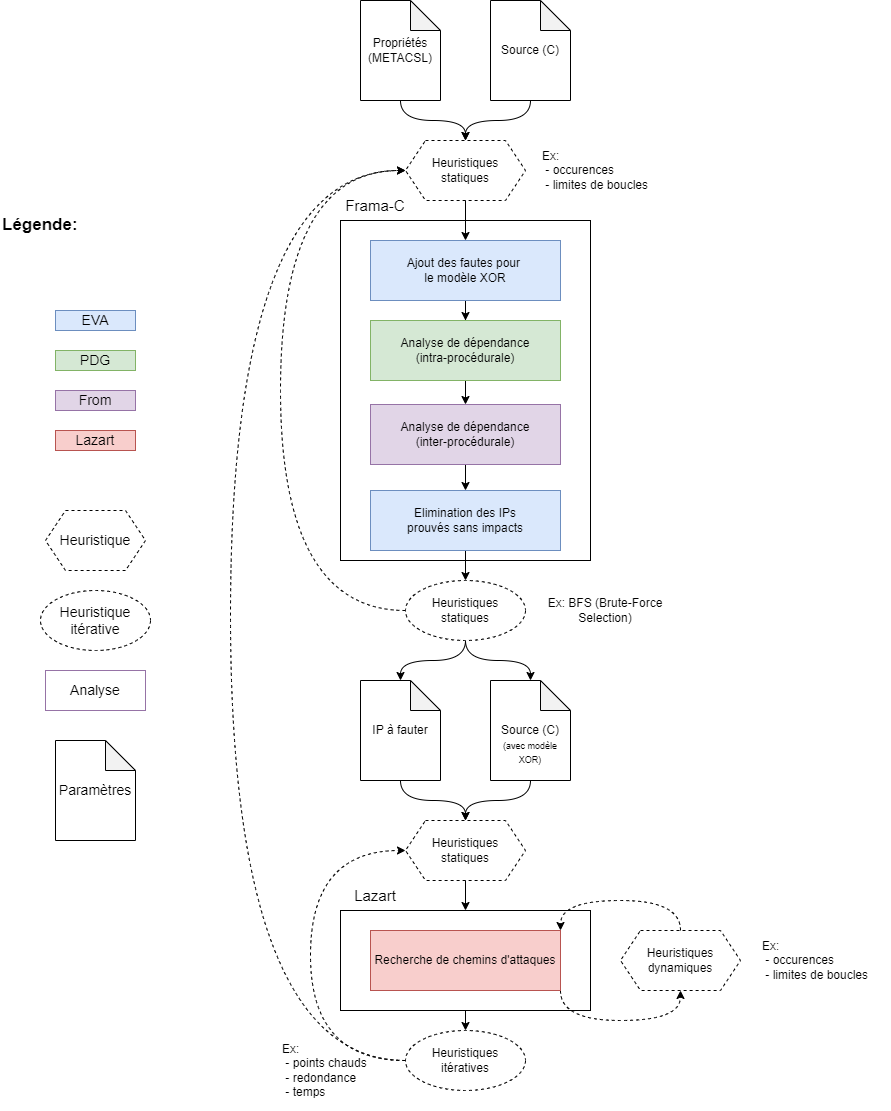
\includegraphics[scale=0.41]{ch3-lazart/img/fdep.drawio.png}
                    \caption{Schéma général de la méthodologie \cite{lacombe2023combining}} \label{fig:metho-fdep}
                \end{figure}
        
                La figure \ref{fig:metho-fdep} présente l'architecture générale de la méthodologie proposée.
                Cette méthodologie utilise l'analyse statique afin de déterminer quels sont les points d'injection qui ont un impact sur la propriété de sécurité étudiée.
                Cet ensemble de fautes est ensuite transmis à Lazart qui recherche des chemins d'attaques.
                Cette approche est présentée dans la section \ref{sec:lazart:metho:eva}.
                Des heuristiques ont aussi été proposées afin de réduire encore l'espace des fautes à injecter. Ces heuristiques peuvent être séparées en deux groupes:
                \begin{itemize}
                    \item Les heuristiques \textit{simples} qui s'appuient sur les résultats d'une unique exécution d'une analyse (section \ref{sec:lazart:metho:static}).
                    \item Les heuristiques \textit{itératives}, qui utilisent une approche itérative pour raffiner le périmètre d'analyse à chaque appel d'un outil, présentées dans la section \ref{sec:lazart:metho:iter}.
                \end{itemize}
                
            \subsubsection{Approximation des points d'injection de fautes utiles}
            \label{sec:lazart:metho:eva}
            
                Cette étape prend en entrée le programme source C et les propriétés à vérifier sous la forme d'assertions (\gls{acsl}). Celles-ci peuvent être définies par l'utilisateur, ou générées automatiquement: les expérimentations conduites utilisent le plugin \gls{rte} de Frama-C permettant de placer automatiquement des assertions contre les erreurs d'exécution.
            
                L'étape d'analyse statique se déroule en quatre sous-étapes:
                \begin{itemize}
                    \item 1) Simulation des points d'injection avec le modèle XOR en introduisant une variable non initialisée (déclarée comme \texttt{extern}) par point d'injection. Cette étape est effectuée avec \gls{eva} qui utilise l'interprétation abstraite (et fonctionne donc par sur-approximation).
                    \item 2) Génération des graphes de dépendances intra-procédural, à l'aide du plugin \gls{pdg} de Frama-C (basé sur \gls{eva}).
                    \item 3) Calcul du graphe de dépendances inter-procédural à l'aide du plugin From.
                    \item 4) Calcul de dépendances pour déterminer quels points d'injection peuvent impacter chaque assertion.
                \end{itemize}
                
                Ainsi, on ne conserve que les points d'injection qui ont un impact (d'après l'analyse de dépendance) sur les assertions non prouvées par \gls{eva}.
                Cette réduction de l'espace de faute préserve la complétude puisque celle-ci est effectuée en considérant toutes les fautes possibles.
                
                La table \ref{tbl:results-fdep} contient les résultats obtenus pour nos programmes de test. La colonne "Nom" indique le programme en question, "IPs" le nombre de points d'injection dans le programme et "Dets" le nombre de points de vérification de contre-mesure (déclenchant un arrêt de la carte si une attaque est détectée).
                La colonne "Lazart (seul)" indique le nombre d'attaques totales trouvées "AP", le nombre de chemins explorés ("EP") et la durée de l'analyse dans le cas où Lazart est lancé sur toutes les fautes générées par le modèle XOR.
                La colonne "AS" correspond à l'étape d'analyse statique (dépendances des propriétés) indiquant le temps d'exécution ("Temps") et le nombre de points d'injection restant après l'analyse ("IPs").
                La colonne Heuristiques indique les heuristiques appliquées ("Type"), le temps d'exécution ("Temps") et le nombre de points d'injection restant après l'application de ces heuristiques ("IPs").
                Enfin, la colonne "Lazart" présente les résultats obtenus avec les points d'injection restants.
                
                Les programmes "vp0" et "vp7" ont été testés sans heuristique (les valeurs \mbox{"-"} indiquant qu'une étape n'est pas effectuée) et permettent d'illustrer un gain de temps non négligeable avec cette analyse de dépendance préliminaire. L'interprétation abstraite passe communément mieux à l'échelle et c'est pourquoi le temps d'analyse reste inférieur à une seconde pour ces exemples.
                Le gain est ainsi bien supérieur pour l'exemple "vp7" qui réduit d'un facteur 10 le nombre de points d'injection à analyser pour Lazart, pour un temps d'analyse trois fois moindre.
                
                \begin{table}[!htpb]
                    \scriptsize
                        \caption{Résultats obtenus pour l'analyse de dépendance}\label{tbl:results-fdep}
                    \begin{center}
                        \setlength\tabcolsep{4pt}
                        \begin{tabular}{l|c|c|c|c|c|c|c|c|c|c|c|c|c}
                        \multicolumn{3}{l|}{Programme} & \multicolumn{3}{l|}{Lazart (seul)} & \multicolumn{2}{l|}{AS} & \multicolumn{3}{l|}{Heuristique} & \multicolumn{3}{l}{Lazart} \\
                        \hline
                        \multicolumn{1}{l|}{Nom} & \multicolumn{1}{l}{IPs} & \multicolumn{1}{l|}{Dets.} & \multicolumn{1}{l|}{AP} & \multicolumn{1}{l|}{EP} & \multicolumn{1}{l|}{Temps} & \multicolumn{1}{l|}{Temps} & \multicolumn{1}{l|}{IPs} & \multicolumn{1}{l|}{Type} & \multicolumn{1}{l|}{Temps} & \multicolumn{1}{l|}{IPs} & \multicolumn{1}{l|}{Attaques} & \multicolumn{1}{l|}{EP} & \multicolumn{1}{l}{Time} \\
                        \hline
                        \hline
                        \multicolumn{1}{l}{vp0} & 20 & 0 & 5 & 65 & \textbf{14s} & 1s & 10 & - & - & - & 5 & 52 & \textbf{11s} \\
                        \multicolumn{1}{l}{vp7} & 142 & 31 & 6 & 3253 & \textbf{1h43} & 1s & 15 & - & - & - & 6 & 1051 & \textbf{30min}
                        \end{tabular}
                    \end{center}
                \end{table} 
                 
            \subsubsection{Heuristiques simples}
            \label{sec:lazart:metho:static}
            
                La méthodologie \cite{lacombe2023combining} propose une heuristique de sélection basée sur le nombre maximal d'occurrences des points d'injection dans une exécution nominale (sans injection de faute).
                Cette heuristique est implémentée avec \gls{eva}, en amont de l'analyse statique de dépendance.
                Cette heuristique fait la supposition qu'un point d'injection qui se déclenche souvent en l'absence de faute, a plus de risque de provoquer une explosion combinatoire des chemins fautés et donc la non-terminaison de l'exploration concolique. 
                Cette heuristique n'est valable qu'en faute unique puisque dans un contexte de fautes multiples, les occurrences des points d'injection peuvent fortement varier.
                
                Une autre heuristique consiste à instrumenter le programme de manière à limiter l'exploration des exécutions.
                Lazart propose des macros d'instrumentation qui coupent l'exploration une fois qu'une limite fixée a été atteinte (par exemple pour limiter les itérations d'une boucle). 
                Lazart n'a cependant pas de solution directe pour définir des limites de fautes différentes pour certains modèles de faute (seule une limite globale de fautes peut être définie). Cela permettrait de limiter l'occurrence de certains points d'injection sans pour autant les ignorer complètement, afin de ne pas passer à côté d'attaques combinées les impliquant. 

                La sélection par force brute (\gls{bfs}) est une heuristique qui a été proposée dans \cite{lacombe2021combining} et qui nécessite plusieurs appels à l'analyseur statique.
                \gls{bfs} consiste à tester indépendamment si un point d'injection a un impact sur les propriétés, en désactivant tous les autres \gls{ip}s. Les points d'injection qui n'ont pas d'impact sur les propriétés sont retirés.
                Cependant, cette approche n'est valide que dans un contexte de faute unique puisque chaque point d'injection est testé indépendamment. Une version multi-fautes nécessiterait d'effectuer autant de fois l'analyse qu'il existe de combinaisons de fautes possibles, ce qui revient à décaler la problématique de l'explosion combinatoire des fautes sur l'analyse de dépendances plutôt que sur l'exécution symbolique.
                La table \ref{tbl:results-fdep2} indique les résultats obtenus avec l'heuristique \gls{bfs} pour l'exemple \textit{iso7816} où près de 60\% des points d'injection peuvent être retirés, en faute unique.
                
            \subsubsection{Heuristiques itératives}
            \label{sec:lazart:metho:iter}
            
                Les heuristiques itératives consistent à raffiner l'espace de faute à injecter au fur et à mesure des analyses. Celles-ci peuvent utiliser l'approche:
                \begin{itemize}
                    \item par \textit{élargissement du périmètre d'analyse}: le périmètre est étendu à chaque itération.
                    \item par \textit{réduction du périmètre d'analyse}: le périmètre est réduit à chaque itération.
                    \item par \textit{combinaison} de réductions et d'élargissement.
                \end{itemize}
                
                Nous avons ainsi proposé une approche par réduction appelée \gls{ss} qui consiste à
                interrompre l'analyse après un temps donné et retirer les points d'injection qui sont les plus déclenchés.
                D'autres métriques produites par l'analyse de points chauds pourraient être considérées pour déterminer les points d'injection à retirer, comme par exemple enlever les points d'injection qui se déclenchent plusieurs fois par attaque (cela étant principalement lié aux boucles).
                Si l'analyse est interrompue mais produit tout de même des attaques, il est possible de retirer les points d'injection apparaissant le plus dans les attaques maximales, puisqu'il s'agit à priori des attaques les moins intéressantes à explorer. 
                Cependant, ces approches par réduction nécessitent de déterminer la durée de seuil du timeout, ce qui n'est pas évident. 
                Dans les cas où seuls quelques points d'injection sont problématiques, ce type d'heuristiques peut fortement aider l'analyse.
                
                L'approche par élargissement que nous avons proposée, appelée \gls{sw}, vise à répéter l'analyse avec Lazart en ajoutant les points d'injection un par un. Si l'analyse dépasse le timeout spécifié lorsqu'un ajoute un point d'injection, alors celui-ci est retiré et un autre point d'injection est testé.
                Il est nécessaire de prévoir une marge par rapport à la durée de l'itération précédente puisque l'ajout d'un point d'injection va nécessairement augmenter le nombre de chemins. Celle-ci a été fixée à 150\% dans nos expérimentations. 
                
                La table \ref{tbl:results-fdep2} présente les résultats obtenus pour les exemples \textit{iso7816} et \textit{sudo}.
                L'exemple sudo a été testé avec la limite des occurrences de points d'injection (réduction) fixée à 1 ("O1") et à 5 ("O5"), et avec l'approche "SW" (élargissement).
                iso7816 a été expérimenté en faute unique avec \gls{bfs} et \gls{sw}, combinée à l'analyse de dépendances (section \ref{sec:lazart:metho:eva}).
                L'approche \gls{bfs}, qui utilise ici un timeout, est très performante car elle réduit très fortement le nombre de points d'injection.
                
                \begin{table}[!htpb]
                \scriptsize
                    \caption{Résultats obtenus pour la méthodologie}\label{tbl:results-fdep2}
                \begin{center}
                    \setlength\tabcolsep{4pt}
                    \begin{tabular}{l|c|c|c|c|c|c|c|c|c|c|c|c}
                    \multicolumn{2}{l|}{Programme} & \multicolumn{3}{l|}{Lazart (seul)} & \multicolumn{2}{l|}{AS} & \multicolumn{3}{l|}{Heuristique} & \multicolumn{3}{l}{Lazart} \\
                    \hline
                    \multicolumn{1}{l|}{Nom} & \multicolumn{1}{l|}{IPs}  & \multicolumn{1}{l|}{AP} & \multicolumn{1}{l|}{EP} & \multicolumn{1}{l|}{Temps} & \multicolumn{1}{l|}{Temps} & \multicolumn{1}{l|}{IPs} & \multicolumn{1}{l|}{Type} & \multicolumn{1}{l|}{Temps} & \multicolumn{1}{l|}{IPs} & \multicolumn{1}{l|}{Attaques} & \multicolumn{1}{l|}{EP} & \multicolumn{1}{l}{Time} \\
                    \hline
                    \hline
                    \multirow{4}{*}{sudo} & 919  & 17 & 737 & 11 & N/A & N/A & \gls{sw} & 23min & 913 & 17 & 737 & 11s \\
                     & 919  & 17 & 737 & 11s & 1s & 104 & \gls{sw} & 3min & 102 & 17 & 670 & 11s \\
                     & 919  & 17 & 737 & 11s & - & - & \gls{sw}+O1 & 3min & 40 & 10 & 602 & 10s \\
                     & 919  & 17 & 737 & 11s & 1s & 104 & \gls{sw}+O5 & 4min & 47 & 10 & 302 & 10s \\
                    \hline
                    \multirow{3}{*}{iso7816} & 153  & - & - & - & -& - & \gls{sw} & 16min & $660 \to 655$  & 1 & 192 & 19s \\
                     & 153  & - & - & - & 153 & 3s & \gls{sw} & 6min  & $153 \to 151$  & 1  & 170 & 12s \\
                     & 153  & - & - & - & 1 & 55s & \gls{bfs} & - & - & 1 & 45 &  1s\\
                    \end{tabular}
                \end{center}
            \end{table} 
        
        \subsection{Périmètre d'analyse de Lazart et analyse partielle}
        \label{sec:rsa-strat}
        
            La méthodologie présentée dans \cite{lacombe2023combining} se concentre sur la sélection des points d'injection sur lesquels une faute pourra être injectée.
            Le modèle XOR englobant la combinaison des modèles d'inversion de test et de données symboliques non contraintes, celui-ci décale la problématique de la sélection des modèles de faute à appliquer vers la problématique de la sélection des points d'injection à activer.
            Comme cela a été évoqué précédemment, le périmètre d'analyse de Lazart inclut aussi d'autres paramètres, notamment le choix de l'objectif d'attaque ou encore de la surface de code à analyser.
            
            Le choix du périmètre d'analyse initial reste une difficulté pour l'utilisateur de l'outil et par exemple, les centres d'évaluation s'appuient en grande partie sur l'expertise des évaluateurs.
            Des méthodes telles que les \textit{stubs}\footnote{Le stub consiste à émuler l'effet d'une partie du programme. Par exemple en remplaçant le corps d'une fonction par un simple retour d'une valeur. Dans ce cas, l'opération est incomplète mais il est possible de préserver la complétude en retournant une variable symbolique dans le cas de Lazart, ce qui revient à faire une sur-approximation des comportements.} peuvent être utilisées pour aider à sélectionner les portions du programme à analyser. L'état de l'art des attaques en fautes permet d'aider à choisir les objectifs d'attaque et modèles de faute à étudier.
            Certains outils d'analyse non liés à l'analyse de fautes peuvent aider à la définition du périmètre d'analyse pour Lazart. Par exemple, l'analyse de dépendances d'\gls{eva} peut permettre ainsi de déterminer quelles fonctions du programme ciblé ont un impact sur les propriétés étudiées et de réduire l'analyse à cette portion.
            Lancer KLEE sur le programme sans injecter de faute (hors de Lazart donc) permet de déterminer si certaines portions du programme posent d'ores et déjà problème pour l'exécution concolique alors qu'aucune faute n'est injectée.
            
            Lorsqu'une analyse est trop complexe pour terminer dans un temps imparti, il est néanmoins possible de récupérer des chemins d'attaques en laissant l'exécution symbolique s'exécuter avec un timeout.
            Dans ce cas, le choix de la stratégie d'exploration est d'autant plus importante que celle-ci peut fortement influer sur les chemins d'attaques qui seront trouvés dans le temps imparti.
            La suite de cette section présente un cas d'utilisation d'une exécution concolique interrompue avec le programme \gls{rsa}.  
           
            Les programmes \gls{rsa} (du \gls{fissc}) n'utilisent pas d'entrées symboliques et utilisent un modèle de mise-à-0 plutôt que la mutation de données symbolique.
            Ces programmes implémentent des opérations modulaires, ce qui implique des boucles dont le nombre d'itérations dépend des entrées.
            Si les entrées ou la valeur d'une faute injectée sont symboliques, alors beaucoup de chemins peuvent être explorés, et potentiellement de longueurs élevées. 
            Néanmoins, il est possible de borner la durée de l'exécution symbolique afin d'obtenir des chemins d'attaques.
            
            La table \ref{tbl:ch3:exp:rsa-strat} présente les résultats obtenus pour le programme d'exemple $rsa0$ avec le modèle d'injection de données en fonction de la stratégie d'exploration utilisée (colonne "Stratégie"). Par défaut, KLEE utilise la stratégie \texttt{nurs-cn} (Non-Uniform Random Search - Coverage-New), visant en priorité les chemins allant vers les instructions les moins couvertes. Les stratégies de recherche en profondeur (\gls{dfs}) et recherche en largeur (\gls{bfs2}) sont également présentées.
            Les colonnes suivantes indiquent le nombre d'attaque réussies trouvées pour chaque nombre de fautes.
            La colonne "EP" correspond au chemins explorés et la colonne "EI" au nombre d'instructions exécutées.
            La colonne "BCov" correspond à la couverture des blocs de base.
            La colonne "TDSE" indique combien de temps l'exécution symbolique a duré\footnote{Le timeout est fixé à 30 minutes mais un temps supplémentaire est nécessaire à KLEE pour générer les ktests correspondant aux chemins en cours d'exploration.}.
            
            \begin{table}[ht]
                \small
                    \caption{Comparaison de différentes stratégies d'exploration}\label{tbl:ch3:exp:rsa-strat}
                \begin{center}
                \setlength\tabcolsep{4pt}
                \begin{tabular}{l|llll|llll}
                Stratégie &1F & 2F & 3F & 4F & EP & EI & BCov & TDSE \\
                \hline
                nurs-cn &  0 & 0 & 0 & 0 & - & - & - & - \\
                dfs &  54 & 71 & 100 & 75 & 419 & 3561393 & 96.8 & 33:37 \\
                bfs &  17 & 18 & 5 & 0 & 95 & 126315 & 33.62 & 57:34:00 \\
                \end{tabular}
                \end{center}
            \end{table} 
            
            On constate que la stratégie d'exploration a un fort impact sur les résultats qui sont obtenus. La stratégie par défaut ne parvient pas à trouver d'attaque en 30 minutes, mais les deux autres stratégies y parviennent, \gls{dfs} trouvant le plus d'attaques dans ce cas. 
            Pour \texttt{nurs-cn}, KLEE ne parvient pas à produire les ktests dans un temps imparti\footnote{Une limite de 1h pour l'arrêt de KLEE a été fixée, mais KLEE ne parvient pas à générer les cas de tests dans le temps imparti et ainsi aucune métrique d'exécution n'est disponible.}.
        
            La table \ref{tbl:ch3:exp:rsa-time} présente les résultats obtenus pour $rsa0$ avec mutation de données symbolique en fonction du temps d'analyse, en utilisant la stratégie d'exploration \gls{dfs}. 
            La colonne "Délai" indique le temps accordé à l'exécution concolique pour l'analyse.
            Les autres colonnes ont la même signification que précédemment (table \ref{tbl:ch3:exp:rsa-strat}). 
            Comme attendu, plus la durée limite est longue, plus l'analyse trouve de chemins d'attaque et plus la couverture est élevée.
            Cela étant, on peut observer que le passage de 1 minute à 5 minutes n'apporte que peu de nouveaux chemins d'attaques (4) tandis que le passage à 30 minutes en ajoute beaucoup.
    
            \begin{table}[ht]
                \small
                    \caption{Attaques trouvées sur RSA en fonction du délai d'analyse spécifié}\label{tbl:ch3:exp:rsa-time}
                \begin{center}
                \setlength\tabcolsep{4pt} 
                    \begin{tabular}{l|llll|lll|l}
                    Délai & 1F & 2F & 3F & 4F & Chemins & Instrs. & BCov & TDSE \\
                    \hline
                    10s & 10 & 5 & 0 & 0 & 35 & 306596 & 90.62 & 00:11 \\
                    1min & 25 & 50 & 50 & 24 & 42 & 1962377 & 93.75 & 01:00 \\
                    5min & 28 & 50 & 50 & 25 & 223 & 1965419 & 96.8 & 05:01 \\
                    30min & 54 & 71 & 100 & 75 & 419 & 3561393 & 96.8 & 33:37
                    \end{tabular}
                \end{center}
            \end{table} 
            
            Le choix de la stratégie d'exploration est un paramètre important pour Lazart, et dans le cas d'analyses qui ne terminent pas en un temps raisonnable, l'utilisation d'un timeout et d'une stratégie d'exploration adaptée permet de tout de même obtenir des résultats. 
            La stratégie d'exploration peut aussi avoir un impact sur la consommation mémoire en fonction du nombre d'états symboliques explorés simultanément.
            Enfin, la stratégie d'exploration est aussi importante dans le cas où l'analyse termine, certaines stratégies pouvant rater des chemins, notamment lorsqu'elle incluent de l'aléatoire.
            
    \section{Conclusion}
        \label{sec:lazart:metho:concl}
        
        La section \ref{lazart:metho} a présenté des solutions et méthodologies permettant de pallier les problématiques liées à l'utilisation de Lazart, notamment en ce qui concerne la sélection des points d'injection à évaluer.
        L'analyse statique permet de réduire l'espace de faute de Lazart de façon considérable sur certains exemples.
        La table \ref{tbl:metho-conclusion} compare certaines des heuristiques présentées précédemment, leur nom étant indiqué dans la première colonne.
        La colonne "Type" détermine si l'heuristique est simple ou itérative. La colonne "Niveau" précise si l'heuristique est appliquée au niveau de l'analyse statique ou de Lazart.
        La colonne "Contexte de fautes" indique si l'heuristique est destinée à la faute unique ou aux fautes multiples et finalement la colonne "Complétude" précise si l'heuristique préserve la complétude.
        
        \begin{table}[hbt]
        \centering
        \caption{Comparaison de différentes heuristiques}
        \vspace{0.2cm}
        {\small
        \label{tbl:metho-conclusion}
            \begin{tabular}{l||l|l|l|l}
            Heuristique & Type & Niveau & Contexte de fautes & Complétude \\
            \hline
            \hline
            Limite d'occurence & simple & \begin{tabular}[c]{@{}l@{}}statique\\ dynamique\end{tabular} & \begin{tabular}[c]{@{}l@{}}simple\\ multiple\end{tabular} & Non \\
            \hline
            Selection bruteforce & iter & statique & simple & Oui \\
            Strategy shrinking & iter & dynamique & simple & Non \\
            Strategy widening & iter & dynamique & multiple & Non \\
            \hline
            Analyse manuelle & both & both & multiple & Non \\ 
            Analyse partielle & both & dynamique & multiple & Non 
        \end{tabular}
        }
        \end{table}
        
        Lazart propose donc des traitements des résultats visant à aider l'utilisateur dans la recherche de vulnérabilité et la protection du programme. 
        Si la définition du périmètre initial d'une analyse reste délicate, l'approche itérative et l'utilisation d'analyse par sur-approximation permettent de guider l'utilisateur.
        
        Le chapitre suivant revient sur ces problématiques du point de vue de l'implémentation. Elle précise certains choix qui ont été faits et qui résultent souvent d'un compromis entre accessibilité, passage à l'échelle et complétude. 
        
\chapter{Lazart - Implémentation et expérimentations}
\label{chpt:lazart-implem}

\begin{tikzpicture}[remember picture,overlay]
\node[anchor=west,inner sep=0pt] at (current page text area.west|-0,3cm) {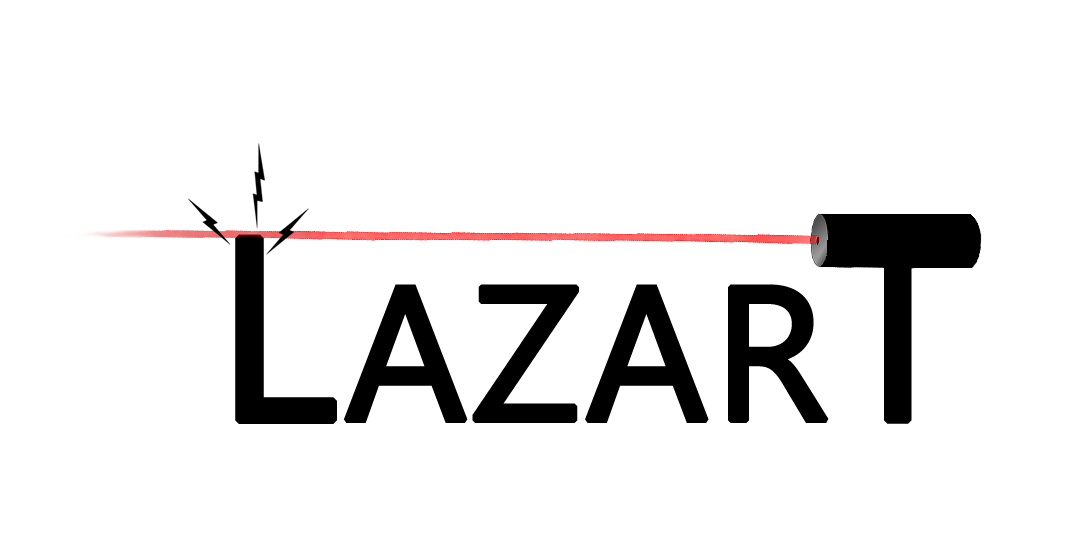
\includegraphics[height=3cm]{ch3-lazart/img/lazart-logo-red.png}};
\end{tikzpicture}

    Ce chapitre s'intéresse à l'implémentation de l'outil Lazart et discute des choix et compromis qui ont été faits.
    
    La section \ref{sec:lazart-impl-klee} décrit l'interaction entre Lazart et l'outil d'exécution concolique (KLEE).
    La section \ref{sec:lazart-impl-wolv} présente Wolverine (phase de mutation), son architecture et son fonctionnement.
    La section \ref{sec:lazart-impl-mfct} explique les choix d'implémentation concernant l'émulation des fautes.
    La section \ref{sec:lazart-impl-analysis} détaille l'implémentation et la complexité des analyses d'attaques de Lazart.
    Finalement, la section \ref{sec:lazart-conclusion} propose une synthèse des chapitres \ref{chpt:lazart} et \ref{chpt:lazart-implem}, ces deux chapitres sur l'outil Lazart et revient sur les contributions et les perspectives de l'outil.

    \setcounter{tocdepth}{2}
    \section*{Table des Matières}
    \localtableofcontents
    
    \section{Interaction avec KLEE}
    \label{sec:lazart-impl-klee}
    
        \begin{figure}[t]\centering
            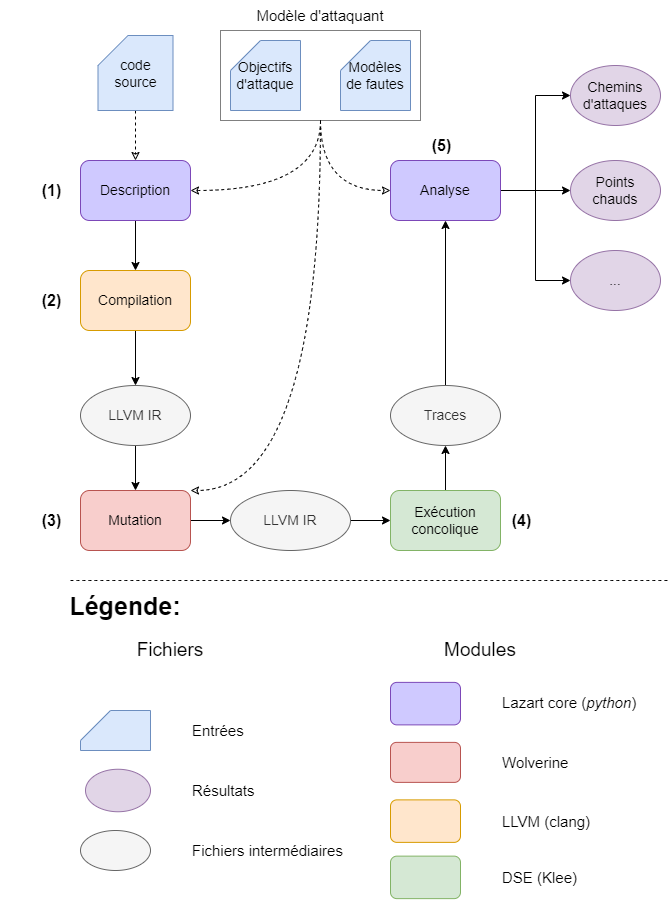
\includegraphics[scale=0.4]{ch3-lazart/img/lazart-workflow4_pack.drawio.png}
            \caption{Processus d'analyse avec Lazart (rappel)}  \label{fig:lazart-analysis-scheme-ch4}
        \end{figure}
    
        KLEE est appelé après la phase de mutation avec pour entrées le mutant \gls{llvm-ir} et des arguments paramétrables depuis l'\gls{api} Python (voir figure \ref{fig:lazart-analysis-scheme-ch4}). Une fois que l'exécution symbolique est terminée (ou bien la fin d'un timeout spécifié par l'utilisateur), la phase de lecture des traces permet de récupérer les résultats de KLEE et les convertir dans la représentation de Lazart.
        L'usage de KLEE nécessite de prendre quelques précautions:
        \begin{itemize}
            \item Retarder au maximum l'introduction de variables symboliques et de disjonction de chemins dues aux fautes.
            \item Couper les traces qui ne nous intéressent pas au plus tôt.
            \item Choisir un paramétrage de KLEE adapté aux besoins de l'analyse et évitant d'introduire une concrétisation non souhaitée.
        \end{itemize}
        
        Ces aspects sont à prendre en compte par l'utilisateur lors de l'instrumentation du programme et du paramétrage de Lazart, comme cela a été abordé dans le chapitre précédent (section \ref{lazart:metho}). 
        Ce sont aussi des problématiques qui ont été considérées lors de l'implémentation de l'outil.
        
        Les deux premiers points sont directement liés à la génération du mutant et à l'émulation des fautes, et seront abordés dans la section \ref{sec:lazart-impl-mfct}. Cette section se concentre sur la récupération des traces d'exécution à partir des cas de test et le paramétrage de KLEE.
        La section \ref{sec:lazart-impl-klee-replay} présente la méthode de rejeu utilisée par Lazart pour récupérer les chemins de KLEE.
        La section \ref{sec:lazart-impl-klee-read} s'intéresse aux optimisations concernant l'exploration des chemins de KLEE et la lecture des ktests par Lazart. 
        La section \ref{sec:userevent} décrit comment récupérer des propriétés sur les traces, par exemple pour vérifier plusieurs objectifs d'attaque en une seule analyse.
    
        \subsection{Rejeu des traces}
        \label{sec:lazart-impl-klee-replay}
 	
            Pour récupérer les données d'une trace à partir d'un cas de test fourni par KLEE (fichier \texttt{.ktest}), chaque évènement d'une trace (entrée dans un bloc de base, déclenchement d'une faute, etc) est affiché sur la sortie standard avec un format spécifique.
            Lazart utilise la fonctionnalité \textit{de rejeu} de KLEE (voir section \ref{sec:klee}) qui permet d'exécuter un ktest avec des entrées concrètes validant le prédicat de chemin de cette trace. La trace est ainsi reconstituée en analysant la sortie console de chaque rejeu de trace et transformée dans la représentation de Lazart.
            
\lstset{caption={Exemple de rejeu d'un ktest de KLEE},label=lst:replay-klee}
\begin{lstlisting}  
[TRACE] bb2
[TRACE] bb3
[FAULT] [DL] [2] [12] [0]
[TRACE] bb5
[USER] tmp = 12
...
\end{lstlisting} 

            Le listing \ref{lst:replay-klee} présente un exemple d'affichage console lors du rejeu d'une trace. 
            Chaque type d'évènement suit une syntaxe précise. Les lignes préfixées par \texttt{[TRACE]} correspondent à l'entrée dans un bloc de base et la ligne préfixée par \texttt{[FAULT]} correspond à l'injection d'une faute dans laquelle le type de modèle est indiqué (ici mutation de données), suivi de l'identifiant du point d'injection (2) et finalement les valeurs spécifiques au modèle (ici la valeur attendue et la valeur fautée).
            
            KLEE propose d'autres outils pour récupérer le chemin d'une trace. L'outil \texttt{ktest-tool} (voir section \ref{sec:klee}) permet de retrouver les valeurs de chaque variable symbolique d'un ktest donné et ainsi récupérer les fautes qui ont été injectées. Cette méthode est utilisée par Lazart lorsque le replay échoue \footnote{Par exemple en cas d'erreur de segmentation lors du rejeu ou bien lorsque le rejeu dépasse un délai fixé.}. Cette méthode permet de retrouver les fautes mais sans ordre et sans information sur le chemin\footnote{La récupération de ces informations depuis KLEE fait partie des perspectives d'amélioration de l'outil.} (fautes non-ordonnées et aucune information sur les blocs de base traversés par exemple).
 	
        \subsection{Lecture des traces}
        \label{sec:lazart-impl-klee-read}
        
            L'étape de lecture des traces consiste donc à rejouer chaque ktest fourni par KLEE pour récupérer le chemin et les fautes injectées.
            La terminaison des traces est obtenue en cherchant les fichiers "*.err" associés à chaque ktest. KLEE génère un fichier par type de terminaison (\textit{klee\_assume} non validé, \gls{rte} par exemple). Si le chemin est complètement exploré, c'est-à-dire que le programme termine de façon nominale avec l'objectif d'attaque validé, alors aucun fichier d'erreur n'est associé au ktest.
            
            Cette étape est très sensible à la performance des accès aux fichiers, d'une part pour le rejeu des traces et d'autre part pour la recherche de la terminaison. Plusieurs optimisations visant à limiter ces accès peuvent être mises en place.
            La récupération de tous les noms de fichiers permet de connaître la terminaison avant d'avoir rejoué la trace, le rejeu nécessitant un accès au fichier et un appel externe à ktest-tool pour chaque trace.
            Cela permet de savoir à l'avance si un ktest correspond à une trace d'attaque réussie et ainsi ne lire que les ktests nécessaires.
            
            La lecture des traces ne lit par défaut que les traces validant l'objectif d'attaque. Ceci peut être paramétré par l'utilisateur s'il souhaite par exemple considérer les \gls{rte} comme des attaques, au prix d'une lecture des traces potentiellement plus longue.
            Néanmoins, KLEE par défaut ne génère qu'un ktest par point de code où une erreur de type \gls{rte} (ptr, div, free etc...), même si plusieurs erreurs se déclenchent dans différents chemins. Par exemple, il ne générera une erreur pour une division par zéro qu'une fois par point de code, même si plusieurs chemins d'attaques peuvent déclencher à ce point du programme.
            Cela permet à KLEE de ne pas effectuer les vérifications (et donc les appels au solveur) concernant les erreurs d'exécution pour chaque chemin.
            L'option \textit{--emit-all-errors} doit être ajouté à KLEE pour générer un cas de test à chaque fois.
            Ainsi, si l'analyse nécessite de récupérer des traces correspondant à des cas d'erreur, il est nécessaire de spécifier l'option correspondante à KLEE et spécifier les ktests supplémentaires à traiter pour Lazart.
            
            La table \ref{tbl:metrics-traces-eae} propose une comparaison de plusieurs configurations de génération de ktests et de traces pour les collections de programmes \texttt{verify\_pin} et \texttt{firmware\_updater} présentés dans le chapitre précédent.
            La colonne "Version" indique les options de KLEE et le mode de génération de traces de Lazart. "eae" indique que tous les cas de tests d'erreur sont générés par KLEE, "standard" indique la lecture des traces standard (objectif d'attaque validé et pas de terminaison en erreur), "rte", la lecture des traces standard plus les erreurs d'exécutions et "full" indique que tous les ktests sont analysés.
            Les colonnes "Traces", "KTests", "EI" et "EP" correspondent respectivement au nombre de traces générées par Lazart, au nombre de Ktests, au nombre d'instructions exécutées et au nombre de chemins explorés.
            Les colonnes suivantes indiquent le temps d'analyse de KLEE ("TDSE"), de lecture des traces ("TTr") et la couverture des blocs de bases ("BCov"), des branches ("BRCov") et des instructions ("ICov").
            
            \begin{table}[h]
                \footnotesize
                \caption{Comparaison des méthodes de génération des traces}
                \label{tbl:metrics-traces-eae}
                \setlength\tabcolsep{3.5pt}
                \begin{center}
                    \begin{tabular}{l|l|l|l|l|l|l|l|l|l|l}
                    Programme & Version & Traces & KTests & EI & EP & TDSE & TTr & BCov & BRCov & ICov \\
                    \hline
                    vp5 & standard & 3291 & 3293 & 2172323 & 14213 & 15.56 & 7.63 & 98.7 & 96.43 & 92.85 \\
                     & rte + eae & 4875 & 14213 & 2172323 & 14213 & 23.65 & 23.146 & 98.7 & 96.43 & 92.85 \\
                     & full + eae & 14213 & 14213 & 2172323 & 14213 & 31.86 & 49.918 & 98.7 & 96.43 & 92.85 \\
                    fu1 & standard & 9179 & 9183 & 36632126 & 137670 & 08:05 & 31.976 & 97.06 & 91.67 & 84.31 \\
                     & rte + eae & 9727 & 137670 & 36632126 & 137670 & 20:34 & 22:20 & 97.06 & 91.67 & 84.31 \\
                     & full + eae & 54305 & 137670 & 36632126 & 137670 & 19:14 & \texttt{02:14:65} & 97.06 & 91.67 & 84.31
                    \end{tabular}
                \end{center}
            \end{table}  
            
            Comme attendu, le mode standard est le plus performant, puisqu'il limite au maximum l'exploration.
            La couverture reste identique dans les exemples considéré quel que soit le mode utilisé, et il en va de même pour les attaques trouvées (qui ne sont pas indiquées ici). 
            L'utilisation de l'option \textit{eae} augmente considérablement le nombre de ktests produits par KLEE, ce qui influe sur le temps de l'exécution symbolique.
            Le temps de l'étape de récupération des traces ("TTr") devient proportionnellement plus important que celui de l'exécution symbolique lorsqu'on augmente le nombre de traces à lire.                
            La couverture reste cependant assez proche de celle obtenue avec l'option \textit{eae}, lorsqu'un ktest est généré pour chaque chemin d'erreur. 
            Le cas \textit{full + eae} implique la lecture de tous les chemins ne validant pas l'oracle, ce qui a peu d'intérêt en pratique mais est donné pour montrer le temps de lecture bien supérieur qu'on obtiendrait. 
        
        \subsection{Objectifs d'attaque multiples et spécification par évènements}
        \label{sec:userevent}
        
            L'utilisation de \textit{klee\_assume} pour la vérification de l'objectif d'attaque permet de trier les traces suivant un prédicat binaire (satisfait / non-satisfait).
            Les \textit{évènements utilisateur} sont une autre méthode de vérification de propriété plus générales sur les traces.
            Cette méthode est notamment utile pour vérifier plusieurs objectifs d'attaque en une seule analyse.
            
            Par exemple, les programmes \textit{verify\_pin} (voir section \ref{sec:lz:exp:bench}) peuvent être analysés avec différents objectifs d'attaques.
            On considérera ici les objectifs $\phi_{auth}$ (s'authentifier avec \gls{pin} faux) et $\phi_{ptc}$ (ne pas décrémenter le compteur d'essai avec un \gls{pin} faux) et leur conjonction $\phi_{auth~\land~ptc}$ et leur disjonction $\phi_{auth~\lor~ptc}$.
            
            S'il est possible d'effectuer une analyse pour chacun des quatre objectifs d'attaque (et donc quatre exécutions concoliques), l'idée ici est d'ajouter des affichages pour le rejeu en fonction des propriétés \textit{auth} (la fonction retourne vrai, l'utilisateur est authentifié) et \textit{ptc} (le compteur d'essais n'a pas été décrémenté). 
            
\lstset{style= codeC, caption={Encodage des propriétés $auth$ et $ptc$ à l'aide d'évènements utilisateurs},label=lst:userevent}
\begin{lstlisting}    
#define _LZ__EVENT(f_, ...) if(klee_is_replay()) { printf(("\n[USER_EVENT] " f_ "\n"), ##__VA_ARGS__); }

int main()
{
    uint8_t user_pin[PIN_SIZE];
    init(user_pin, card_pin); // make symbolic and not-equal

    BOOL ret = verify_pin(user_pin);

    if(ret == TRUE) {
        _LZ__EVENT("AUTH");
    }
    if(try_counter >= TRY_COUNT) {
        _LZ__EVENT("PTC");
    }
    return 0;
}
\end{lstlisting}
    
            Le listing \ref{lst:userevent} présente l'encodage des propriétés \textit{auth} et \textit{ptc} avec des \textit{évènements utilisateur}, la non-égalité des entrées étant toujours vérifiée à l'aide d'un appel à \texttt{klee\_assume} (dans la fonction \texttt{init}).
            Plutôt que couper les traces qui ne vérifient pas un objectif d'attaque binaire (avec \texttt{klee\_assume}), des évènements utilisateurs (ici \textit{AUTH} et \textit{PTC} sont ajoutés à la liste des transitions des traces en fonction des propriétés \textit{auth} et \textit{ptc}.
            La macro \texttt{\_LZ\_\_EVENT} englobe un appel à \textit{printf} avec le bon format pour que l'évènement utilisateur soit récupéré lors du rejeu (l'implémentation de cette macro est indiqué ligne 1). 
            
\lstset{language=python, caption={Encodage des propriétés de l'objectif d'attaque à l'aide d'évènements utilisateurs},label=lst:userevent-py}
\begin{lstlisting}    
execute(a, no_analysis=True) # Compile, mutate, run DSE and parse traces

print(attacks_results(a, satisfies_fct=lambda trace: trace.satisfies() and trace.has_event("AUTH"))
print(attacks_results(a, satisfies_fct=lambda trace: trace.satisfies() and trace.has_event("PTC"))
print(attacks_results(a, satisfies_fct=lambda trace: trace.satisfies() and trace.has_event("AUTH") and trace.has_event("PTC"))
print(attacks_results(a, satisfies_fct=lambda trace: trace.satisfies() and trace.has_event("AUTH") or trace.has_event("PTC"))
\end{lstlisting}

            Le listing \ref{lst:userevent-py} présente le code Python dans le script d'analyse permettant d'effectuer les analyses d'attaques sur les quatre objectifs d'attaque. Pour chaque analyse, les traces sont filtrées en fonction de la présence des évènements.
            L'analyse $a$ est exécutée sans analyse d'attaque (\textit{no\_analysis=True}) puis une analyse d'attaque est exécutée pour chaque objectif d'attaque, en utilisant un filtrage des traces différent (\textit{satisfies\_fct}).
            
            La table \ref{tbl:vp-oracles} présente les résultats d'une analyse du programme $vp3$ pour les quatre objectifs d'attaque, en fonction de la méthode de vérification de l'oracle. Le programme est analysé avec le modèle d'inversion de test avec une limite de 5 fautes et des tableaux d'entrée symboliques.
            La colonne "Version" indique si l'analyse vérifie un objectif d'attaque "binaire" ou à l'aide d'évènements utilisateur ("uevent"). La colonne "objectif" indique l'objectif d'attaque étudié, "total" correspondant au total des analyses séparées pour la version "binaire".
            La colonne "chemins" correspond au nombre de chemins explorés et la colonne "instrs." correspond au nombre total d'instructions exécutées. 
            Les colonnes "ICov" et "Bcov" indiquent respectivement la couverture des instructions et des blocs de base et "TDSE" et "TTot" indiquent respectivement la durée d'exécution concolique de l'analyse et la durée totale.
            
            \begin{table}[h]
                \caption{Résultats des l'analyses en fonction de la méthode de calcul de l'objectif d'attaque}
                \label{tbl:vp-oracles}
                \small
                \begin{center}
                \begin{tabular}{l|l|l|l|l|l|l|l}
                Version & Objectif & Chemins & Instrs. & ICov & BCov & TDSE & TTot \\
                \hline
                séparée & $\phi_{auth}$ & 1930 & 199238 & 98.01\% & 94.64\% & 1s 32 & 3s 305 \\
                 & $\phi_{ptc}$ & 1930 & 192652 & 97.99\% & 94.64\% & 1s 19 & 3s 124 \\
                 & $\phi_{auth\land~ptc}$ & 1930 & 205825 & 98.03\% & 94.64\% & 1s 47 & 3s 237 \\
                 & $\phi_{auth\lor~ptc}$ & 1930 & 205826 & 98.03\% & 94.64\% & 1s 19 & 3s 179 \\
                 & total & 7720 & 803541 & - & - & 5s 17 & 12s 75 \\
                \hline
                uevent & tous & 1930 & 206953 & 97.53\% & 92.19\% & 1s 37 & 5s 955
                \end{tabular}
            \end{center}
            \end{table} 
        
            On constate que les \textit{évènements utilisateurs} permettent d'améliorer grandement le temps d'analyse par rapport à l'utilisation d'analyse séparées avec des objectifs d'attaque binaires. 
            Le surcoût de complexité de l'exécution concolique pour la vérification des différentes propriétés est largement compensé par l'usage d'une seule exécution concolique. On constate en effet que 1930 chemins sont explorés dans tous les cas, l'utilisation d'analyses séparées répète l'exploration de certains chemins. 
            Dans cet exemple, les mêmes chemins d'attaque sont trouvés pour chaque objectif d'attaque binaire avec les deux méthodes.
            Néanmoins, il faut prendre en compte que la complexité supplémentaire de la vérification des différentes propriétés peut potentiellement faire rater des chemins d'attaque au moteur d'exécution concolique.
            
            Les évènements utilisateurs permettent d'analyser plusieurs objectifs d'attaque en une seule exécution concolique, et plus généralement sont utilisés pour obtenir des propriétés plus complexes qu'un prédicat binaire (satisfait/non-satisfait) sur les traces.
        
    \section{Phase de mutation - Wolverine}
    \label{sec:lazart-impl-wolv}
    
        L'étape de mutation (étape 3 de la figure \ref{fig:lazart-analysis-scheme-ch4}) est réalisée avant la phase d'exécution concolique par le module \textit{Wolverine} de Lazart. La représentation intermédiaire issue de la compilation est mutée de manière à y introduire la possibilité d'injecter des fautes.
        Cette phase de mutation est effectuée en fonction de la description du modèle d'attaquant et des opérations à effectuer dans le \textit{fichier de mutation} au format \gls{yaml}.
        Le format de ce fichier est détaillé dans la section \ref{sec:lazart-impl-mutation-file}. 
        
        Wolverine utilise l'\gls{api} C++ de \gls{llvm} permettant la manipulation de la représentation intermédiaire et s'appuie également sur une bibliothèque C liée au programme à analyser au moment de la compilation (étape 2). Il prend en entrée le programme sous la forme d'un bytecode \gls{llvm} (.bc) et le fichier de mutation \gls{yaml}, et vise à transformer chaque point d'injection du programme, par une transformation qui simule l'effet d'une faute (en fonction du modèle de faute spécifié) si le booléen symbolique d'injection est vrai. 
        
        \begin{figure}[ht]\centering
          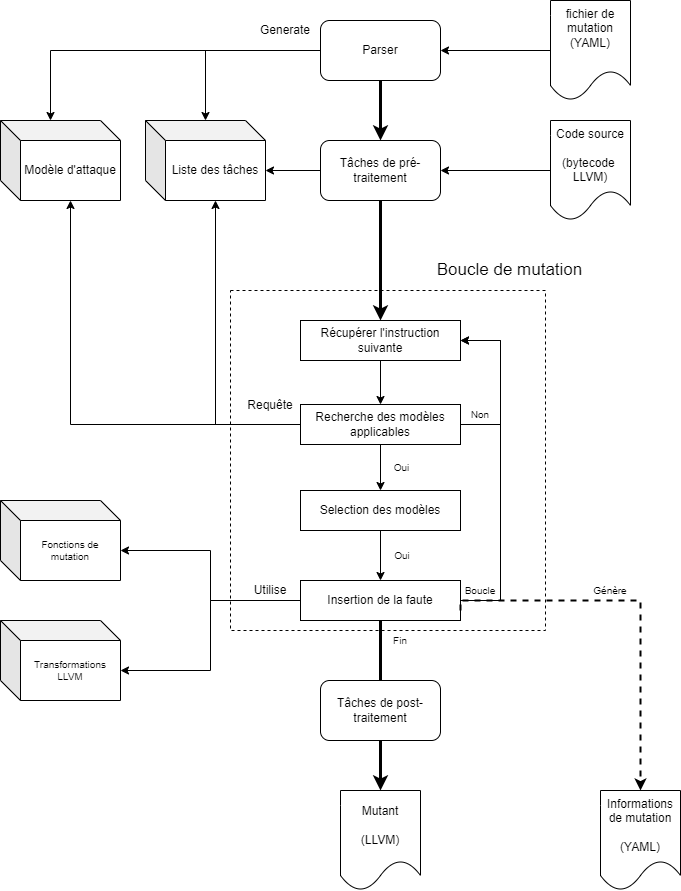
\includegraphics[scale=.52]{ch3-lazart/img/wolverine4-fr.drawio.png}
          \caption{Schéma général de \textit{Wolverine}  \label{fig:wolverine}}
        \end{figure}
        
        La figure \ref{fig:wolverine} présente le fonctionnement général d'une mutation.  
        Après la génération du modèle d'attaquant à partir du fichier de mutation (étape 1), l'étape de \textit{pré-traitement} (étape 2) consiste en plusieurs parcours du programme en fonction des opérations définies par l'utilisateur dans le fichier de mutation et l'instrumentation (détaillée en section \ref{sec:lazart-impl-preprocess}). 
        
        La \textit{boucle de mutation principale} parcourt chaque instruction du programme, fonction par fonction et bloc de base par bloc de base. Pour chaque instruction, le modèle d'attaquant et les informations des analyses sont interrogés afin d'obtenir la liste des modèles de faute applicables sur cette instruction. Le programme est transformé en fonction des modèles de faute sélectionnés. Ces transformations sont détaillées dans la section \ref{sec:lazart-impl-ip-transf}.
        Enfin, Wolverine génère le fichier \gls{llvm-ir} mutant qui sera transmis à KLEE. Il génère aussi certaines informations utilisées ensuite par Lazart, telles que la liste des points d'injection.
        
        \subsection{Fichier de mutation}
            \label{sec:lazart-impl-mutation-file}
            
            Le fichier de mutation contient les paramètres de la mutation sous la forme d'un fichier \gls{yaml} qui est soit fourni par l'utilisateur, soit généré depuis Lazart Core lorsque ceux-ci sont décrits directement en Python. Le listing \ref{lst:mutation-file-example-} montre un exemple de fichier de mutation.
                
\lstset{caption={Exemple de fichier de mutation},label=lst:mutation-file-example-}
\begin{lstlisting}  
---
# Example of mutation file for Wolverine
tasks: # Preprocessing tasks
  add_trace: 
    on: __mut__
  rename_bb: 
    on: __all__
  countermeasures:
    - on: __mut__
      type: load-duplication
## General fault models, can be reused on specific location by ID.
fault-models:
  - &data
    type: data
    all: 0 # All load are faulted to 0.
## Fault spaces. Uses fault models on specific location of the program.
fault-space:
  functions:
    __all__:
      models: [*data]
    foo:
      models: 
        - type: test-inversion
\end{lstlisting} 

            Le fichier de mutation contient trois parties: la section des tâches de pré-traitement (\texttt{tasks} ligne 3), la section des modèles de faute (\texttt{fault-models} ligne 12) et la section d'espace de faute (\texttt{fault-spaces} ligne 17). 
            La section des tâches contient un ensemble d'actions effectuées en pré-traitement ou post-traitement. Dans l'exemple \ref{lst:mutation-file-example-}, les tâches \texttt{add-traces} (l'ajout des \texttt{printf} de trace d'exécution), \texttt{rename-bb} (renommage des blocs de base) et \texttt{countermeasures} (application d'une contre-mesure, ici la duplication des \texttt{load}) sont définies. Le champ \texttt{on} définit l'ensemble des fonctions sur lesquelles la tâche est effectuée, \texttt{\_\_mut\_\_} et \texttt{\_\_all\_\_} étant des mots clefs prédéfinis correspondants respectivement à l'ensemble des fonctions sur lesquelles au moins un modèle est défini et l'ensemble de toutes les fonctions.
            
            La section de l'espace de faute suit une structure identique à celle du champ \texttt{attack\_model} (modèle d'attaquant) de l'\gls{api} Python (voir section \ref{sec:lazart-am-py}) et contient une association entre des points du programme (ici des fonctions) et des modèles de faute. Ces modèles peuvent être définis en-place ou par référence \gls{yaml} (comme ligne 20 dans l'exemple: \texttt{[*data]}).

        \subsection{Phase de pré-traitement}
        \label{sec:lazart-impl-preprocess}
        
            La phase de pré-traitement est effectuée au début de la passe de mutation. Celle-ci applique un ensemble d'opérations en fonction du fichier de mutation.
            
            Les opérations utilitaires (renommage de blocs de base), de trace (ajout de \texttt{printf} pour tracer les blocs de base pour l'étape de rejeu) ou encore d'ajout de contre-mesures automatiques sont appliquées lors de cette phase avec une granularité de l'ordre de la fonction ou du bloc de base. 
            Le pré-traitement effectue aussi les opérations déterminées par l'instrumentation du programme.            
            
            Cette phase pourrait aussi être utilisée pour appliquer d'autres analyses préliminaires (comme celles décrites dans la section \ref{lazart:metho}).
            Dans la première version de l'outil \cite{Potet/ICST14}, le modèle d'inversion de test était précédé par une phase de "coloration de graphe" effectuée dans un module externe en Java permettant de réduire l'espace de faute. 
            L'objectif d'attaque était alors défini en termes d'accessibilité à un bloc précis et cette analyse consiste à colorer chaque bloc pour savoir si une faute en inversion de test vers les branches then, else ou les deux peut mener au bloc ciblé.
            La combinaison de modèles de faute et la gestion de l'inter-procédural compliquent l'analyse dans les versions modernes de Lazart mais il s'agit aussi d'une analyse qui pourra être implémentée dans la phase de pré-traitement.
            
        \subsection{Boucle de mutation et points d'injection}
        \label{sec:lazart-impl-ip-transf}
        
            La boucle de mutation effectue une passe sur toutes les instructions du programme dans les fonctions spécifiées par le modèle de faute comme présenté dans la figure \ref{fig:wolverine}.
            Elle maintient en parallèle l'état des indications de l'instrumentation en fonction des primitives rencontrées dans le programme, telles que l'activation ou la désactivation de modèles (voir section \ref{sec:lazart-am-instr}).
            
\lstset{caption={Boucle de mutation de Wolverine},language=python, label=lst:wolv-mut-loop}
\begin{lstlisting}  
def mutation_loop(module: LLVMModule, istate: InstrumentationState, am: AttackModel):
    for function in llvm_module:
        istate.reset_function();
        for bb in basic_block:
            istate.reset_bb();
            for instr in bb:
                consumed = istate.handle(instr)
                if consumed:
                    continue
                    
                models = am.get_appliable_models(instr, istate)
                if len(models) > 0:
                    model = models[0]
                    if len(models) > 1: 
                        warning("several models appliable, selecting: " + model)
                    (instr, bb) = models.apply(instr)  
\end{lstlisting}

            Le listing \ref{lst:wolv-mut-loop} présente le pseudo-code de la boucle de mutation principale de Wolverine. Toutes les fonctions sont parcourues (à l'exception de primitives de \gls{llvm} et de Lazart) afin de pouvoir y détecter une activation de modèle par l'instrumentation\footnote{Le surcoût de performances est négligeable, toute l'étape de mutation étant elle-même négligeable.}.
            Comme le montre l'avertissement à la ligne de 15, Lazart considère que plusieurs modèles applicables sur une même instruction correspond à une erreur de configuration (par exemple si deux modèles de mutation de donnée s'appliquent sur une même variable). La section \ref{sec:wolverine-multi-ip} revient sur les cas où plusieurs fautes peuvent survenir sur un même point du programme.
            
            Une difficulté de la combinaison de modèles de faute est qu'il ne faut pas qu'un modèle s'applique sur du code qui est relatif à l'analyse (code de simulation des fautes, \texttt{printf} pour le rejeu etc.) et non au programme analysé.
            L'utilisation d'une seule passe permet de ne jamais muter deux fois une instruction (dès lors que les transformations sont locales) mais Wolverine utilise par ailleurs un système d'étiquettes sur les instructions lui permettant d'identifier quelles instructions sont relatives à un point d'injection, à une contre-mesure ou à l'affichage du rejeu par exemple.
            
            Wolverine fait le choix de limiter un maximum l'impact de la mutation sur le graphe de flot et le code original en englobant le code de déclenchement des points d'injection dans des \textit{fonctions de mutation} (section \ref{sec:lazart-impl-mfct}). 
            Ce choix permet aussi de simplifier le code muté s'il doit être utilisé par d'autres outils ou examiné manuellement, en permettant d'identifier simplement les parties du programme correspondant aux points d'injection.
            Cela étant, cette sur-couche d'un appel de fonction peut avoir des conséquences sur les performances de KLEE (discuté dans la section \ref{sec:lazart-mfct-inl}). 

            Le listing \ref{lst:llvm-mutable} contient un exemple de code \gls{llvm-ir} qui va permettre d'illustrer le fonctionnement de ces fonctions. Le listing \ref{lst:llvm-mutable-c} donne l'équivalent C de ce programme. 
            
            \begin{minipage}{0.93\linewidth}
            \begin{lstlisting}[style=base, caption={IR LLVM source}, label=lst:llvm-mutable]
µ%1 = load i32* %val, align 4µ            ; lecture de val
%2 = call i32 @foo(i32 %1)              ; appel de foo
%3 = icmp ne i32 %2, 0                  ; comparaison
§br i1 %4, label %else, label %then§      ; branchement conditionnel

\end{lstlisting}      
                
            \begin{lstlisting}[style=base, caption={Équivalent en langage C}, label=lst:llvm-mutable-c]
if(foo(val)) {
  // then:
} else {
  // else:
}
            \end{lstlisting} 
            \end{minipage}
            
            Dans cet exemple, pour un modèle de faute de mutation de donnée, la ligne 1 du programme est un point d'injection où la faute revient à charger une autre valeur que celle de \texttt{\%val}. De la même manière, une faute dans le modèle d'inversion de test peut être représentée par la négation de la condition de l'instruction \texttt{br} ligne 4. Ces deux points d'injection sont nommés respectivement $IP_{data}$ et $IP_{ti}$. 
         
            \begin{minipage}{0.93\linewidth}
            \begin{lstlisting}[style=base, caption={IR LLVM muté}, label=lst:llvm-mutated]
[...]
µ%6 = alloca i32
%7 = load i32* %val, align 4
%_LZ__w_call_ip_1 = call i32 @_LZ__mut_dl_i32(i32 %7, i8* getelementptr inbounds ([2 x i8], [2 x i8]* @_LZ__w_ip_1_id, i32 0, i32 0))
store i32 %_LZ__w_call_ip_1, i32* %6, align 4
%8 = load i32* %6, align 4µ
%9 = call i32 @foo(i32 %8)
%12 = icmp ne i32 %9, 0
§%_LZ__w_call_ip_2 = call i32 @_LZ__mut_ti(i32 %12, i8* getelementptr inbounds ([2 x i8], [2 x i8]* @_LZ__w_ip_1_id, i32 0, i32 0), i8* getelementptr inbounds ([5 x i8], [5 x i8]* @_LZ__w_ip_0_targetA, i32 0, i32 0), i8* getelementptr inbounds ([5 x i8], [5 x i8]* @_LZ__w_ip_0_targetB) 
br i1 %_LZ__w_call_ip_2, label %bb26, label %bb25§
            \end{lstlisting}
            \end{minipage}
            
            Le listing \ref{lst:llvm-mutated} présente la transformation du programme \ref{lst:llvm-mutable} à l'aide de fonctions de mutation pour les points d'injection $IP_{data}$ et $IP_{ti}$, respectivement représentés en rouge et en bleu-vert.
            Les fonctions de mutation (ici \texttt{\_LZ\_\_mut\_dl\_i32} et \texttt{\_LZ\_\_mut\_ti}) prennent en argument la valeur originale de l'opérande cible, une chaîne de caractère correspondant à l'identifiant (unique) du point d'injection et d'éventuels arguments supplémentaires nécessaires au modèle.
            L'opérande de l'instruction ciblée est passée à la fonction de mutation dont le retour est utilisé comme nouvelle opérande. 
            
            Dans le cas de la mutation de donnée, une variable temporaire est créée puisque la valeur non fautée $\%val$ doit être chargée avant d'être passée à la fonction de mutation, et l'instruction \texttt{load} ligne 6 nécessite une adresse (\texttt{i32*}) comme opérande. Cette valeur temporaire est ainsi créée avec l'instruction \textit{alloca} ligne 2, initialisée ligne 3, et finalement le retour de fonction \texttt{\%\_LZ\_\_w\_call\_ip\_1} est stocké dans la valeur temporaire avec une instruction \texttt{store} ligne 5, puis utilisé comme opérande pour l'instruction \texttt{load} ciblée par la faute ligne 6. Ainsi, il n'est pas nécessaire de modifier toutes les instructions du programme qui utilisent le temporaire \texttt{\%8} puisque celui-ci reste inchangé.

            Le modèle \gls{JMP} n'est pas géré nativement par Wolverine et la transformation de leurs points d'injection est effectuée à la compilation via l'instrumentation.
            Le modèle est cependant reconnu durant la boucle de mutation afin de supporter les points d'injection générés par l'utilisateur dans les analyses (l'\gls{api} Python ayant accès à ces points d'injections via le fichier \texttt{injection\_points.yaml}). 
                
    \section{Émulation des fautes}
    \label{sec:lazart-impl-mfct}
    
        Cette section s'intéresse à l'implémentation de l'émulation des fautes, que ce soit dans les fonctions de mutation ou dans les transformations de points d'injection.
        L'objectif de ces transformations est de retarder l'introduction des variables symboliques ainsi que les disjonctions de chemins et de couper au plus tôt l'exploration des chemins.
        
        La section \ref{sec:lazart-mfct-base} présente la structure des fonctions de mutation et propose une comparaison de plusieurs approches.
        La section \ref{sec:lazart-mfct-data} se concentre sur le modèle de mutation de données symboliques qui inclut une variable symbolique supplémentaire et discute des différentes versions de fonctions de mutation utilisées.
        La section \ref{sec:lazart-mfct-inl} discute des problématiques induites par les fonctions de mutation par rapport à une transformation en-place et des différentes solutions.
        La section \ref{sec:wolverine-multi-ip} parle de l'implémentation des points d'injection multiples générés par l'instrumentation.
 
        \subsection{Fonctionnement}
        \label{sec:lazart-mfct-base}
            
                Le programme présenté dans le listing \ref{lst:mfct-base} correspond au pseudo-code d'une émulation de faute sous la forme d'une fonction de mutation. 
                Les entrées sont la valeur originale \texttt{orig}, potentiellement symbolique, le compteur de fautes \texttt{fcount} (symbolique). La limite de fautes \texttt{flimit} est globale. 
                Les différents prédicats de chemins sont indiqués en marron et la mémoire symbolique (indiquée en rouge) considère \texttt{orig} comme concrète en entrée pour cet exemple.
                
             \begin{center}
            \lstset{basicstyle=\large}
            \lstset{language=C,style=codeC}    
            \begin{lstlisting}[caption=Pseudo-code de l'émulation des fautes, escapeinside={(*}{*)}, language=python, label=lst:mfct-base]
def mutation_fct(orig, fcount): (*{\color{brown} $PC_0 \equiv PC_{fcount}$ }*) (* {\color{red} $\sigma \: = \: \{ \: fcount \: \to \: fcount_0 \}$}*)
    if fcount >= flimit: # No sym variable. (*{\color{brown} $PC_1  \equiv PC_0 \land fcount \geq flimit $}*)
        return orig      
    (*{\color{brown} $PC_2 \: \equiv \: PC_0 \land fcount < \: flimit $}*)
        
    inject = sym_bool() # New sym variable.  (* {\color{red} $\sigma \: = \: \{ \: fcount \: \to \: fcount_0 \: \land \: inject = inject_0 \}$}*)
    if inject: (*{\color{brown} $PC_3  \equiv PC_2 \land inject = true $}*)
        fcount++ # Update. (* {\color{red} $\sigma \: = \: \{ \: fcount \: \to \: fcount_0 + 1\: \land \: inject = inject_0 \}$}*)
        if klee_is_replay(): # Do not create new paths.
            print(fault_str_with_params) # Trace fault trigger for replay.
        return faulted_value
    (*{\color{brown} $PC_4  \equiv PC_2 \land inject = false $}*)

    return orig
                \end{lstlisting}    
            \end{center}     

            Cette implémentation vise à retarder au maximum la création de la variable symbolique booléenne \texttt{inject}. C'est pourquoi un premier test sort immédiatement de la fonction si la limite de fautes est atteinte. C'est aussi la raison pour laquelle \textit{klee\_assume} n'est pas utilisée ici, son appel n'étant pas possible avant la création d'\texttt{inject}.
            La fonction \textit{klee\_is\_replay} est une primitive de KLEE permettant de ne pas exécuter le code lié au rejeu des traces durant l'exécution concolique, qui évite les risques de concrétisation \footnote{La documentation de KLEE indique que la fonction \texttt{printf} est gérée de façon spéciale, de manière à ne pas introduire de concrétisation. Mais nos expérimentations ont mit en évidence certains cas où la présence d'un appel à \texttt{printf} dépendant de variables symboliques fait manquer des chemins à KLEE.}.
 	
        \subsection{Mutation de données}
        \label{sec:lazart-mfct-data}
            
            Cette section vise à présenter les différentes approches d'émulation de fautes en données.
            Le listing \ref{lst:mut-data} présente le pseudo-code du retour de la valeur dans le cadre d'une faute des cinq approches d'implémentation de la fonction de mutation pour l'injection sur les données:
            \begin{itemize}
                \item \texttt{sym}, la variable symbolique injectée n'est pas contrainte et est retournée directement.
                \item \texttt{sym\_pred}, la fonction retourne un booléen déterminant si la valeur est valide, et qui est vérifié par un appel à \texttt{klee\_assume}. 
                \item \texttt{sym\_fun}, la valeur est transformée par la fonction qui retourne une nouvelle valeur contrainte.
                \item  \texttt{fun}, consiste à faire la même opération sans passer par une valeur symbolique.
                \item \texttt{fixed}: est utilisée pour l'injection d'une valeur constante.
            \end{itemize} 
                
\lstset{language=python, caption={Différentes versions de contraintes la mutation de donnée},language=python,label=lst:mut-data}
\begin{lstlisting}   
# Symbolic raw (sym)
return sym_int()
    
# Symbolic constrained (sym_pred)
value = sym_int()
klee_assume(pred(value, original))
return value;

# Symbolic constrained (sym_fun)
value = sym_int()
return f(value, original)
    
# Not symbolic, apply function (fun)
return f(original)
    
# Fixed value (fix)
return N
                \end{lstlisting}

            
  
        \subsection{Performance et inlining}
        \label{sec:lazart-mfct-inl}
 	
 	        Cette section compare les approches par fonction de mutation et par transformation en-place (c'est-à-dire sans appel de fonction, en transformant le graphe de flot local).
 	        Les fonctions de mutation ont l'avantage d'être plus simples pour un utilisateur qui souhaiterait créer de nouveaux modèles et parce qu'elles simplifient le code à analyser en séparant clairement le graphe de flot original de la partie mutation.
 	        Cependant, ces fonctions induisent une surcharge pour le moteur d'exécution symbolique, qui doit effectuer le changement de contexte dû à un appel de fonction et transmettre des paramètres statiques en argument (comme la chaîne de caractères correspondant à l'identifiant de point d'injection, ou l'entier \texttt{fcount} correspondant au nombre de fautes injectées par exemple), et les auteurs de REFINE \cite{Georgakoudis/ICHPCNSA17} indiquent que l'implémentation en-place permet d'obtenir des meilleures performances.
 	        Néanmoins, les expérimentations menées pour Lazart monstrent que ce surcoût n'est pas si important dans le cas d'une exécution concolique avec KLEE, l'explosion des chemins due aux fautes ayant un impact bien plus important que cette surcharge sur certains exemples.
 	        
            Wolverine propose une option d'inlining automatique des fonctions de mutation via une passe \gls{llvm} qui est par défaut appliquée sur chaque appel de fonction de mutation (généré ou défini par l'utilisateur). Cette approche n'effectue pas un inlining en-place, mais place le code de la fonction de mutation dans la fonction courante (qui est donc réutilisé par d'autres injections dans la même fonction). Cette approche souffre de la surcharge de la transmission des arguments tout comme la version avec fonction de mutation, mais ne contient pas d'appel de fonction explicitement (instruction \texttt{call}).
            Une version en-place de la mutation de donnée symbolique a aussi été implémentée, qui elle consiste à avoir un code de mutation séparé pour chaque point d'injection.
            
            La table \ref{tbl:inlining} compare l'approche des fonctions de mutation sans optimisation (\texttt{mfct}), l'inlining automatique (\texttt{mfct+inl}) et la mutation en-place (\texttt{inplace}) sur un ensemble de programmes. Les exemples utilisés sont indiqués dans la colonne "Prgm.", $rsa0$ correspondant à l'implémentation de \gls{rsa} en mise-à-0 et $loader$ au bootloader (voir chapitre précédent). $loader$ n'est évalué qu'en faute unique.
            L'approche utilisée est indiquée dans la colonne "Stratégie", la version en-place n'étant pas implémentée pour l'injection d'une valeur fixe, la version en-place pour $rsa0$ n'est pas présente.
            Les colonnes suivantes indiquent le nombre d'attaques trouvées en fonction du nombre de fautes. On constate que chaque version donne bien des résultats identiques. 
            
            Les colonnes "Chemins" et "Instrs." indiquent respectivement le nombre de chemins explorés et le nombre d'instruction exécutées. On constate que l'inlining automatique est moins performant.
            La colonne "TDSE" qui indique le facteur de temps d'exécution moyen indexé sur l'approche la plus faible. Les variations entre les versions \texttt{mfct} et \texttt{mfct+inl} sont trop faibles pour être mesurées dans le cas de $rsa0$ mais visibles sur $loader$. 
            Le fait que l'inlining automatique soit plus coûteux tend à montrer que les changements de contexte lié à l'appel de fonction sont négligeables pour KLEE. La différence entre les deux étant expliquée par le fait que l'inlining automatique de \gls{llvm} complexifie légèrement le graphe de flot.
            En revanche, l'exemple $loader$ indique des facteurs de temps plus significatifs. La version \texttt{inplace} étant la plus performante puisque les passages d'arguments ne sont pas présents.
            
            Les colonnes "ICov" et "BCov" donnent des indications concernant la couverture des instructions et des blocs de base. La différence entre les approches est significative mais principalement parce que ces métriques ne mesurent pas la même chose suivant les versions.
            Dans le cadre d'une approche \texttt{mfct}, chaque point d'injection partage son code avec tous les points d'injection utilisant la même fonction de mutation. La couverture donnée par KLEE reflète donc davantage celle obtenue sur le programme analysé.
            Dans le cadre de l'inlining automatique \texttt{mfct+inl}, la couverture du code d'émulation est liée à la fois à la fonction de mutation utilisée, mais aussi à la fonction contenant le point d'injection.
            Pour la mutation en-place, le code d'émulation est séparé pour chaque point d'injection et la couverture retournée par KLEE est donc plus faible.
            On constate d'ailleurs que le nombre de chemins explorés est le même pour toutes les approches, seul le nombre d'instructions exécutées diffère.
            
            \begin{table}[ht]
            \centering
            \small
            \setlength\tabcolsep{4pt} % default value: 6pt
            \begin{tabular}{l|l|llll|lll|lll}
            Prgm. & Stratégie & 1F & 2F & 3F & 4F & Ktests & Chemins & Instrs. & ICov & BCov & TDSE \\
            \hline
            \hline
            rsa0 & mfct & 10 & 33 & 65 & 92  & 202 & 913 & 52965525 & 100 & 100 & \textbf{1} \\
            & mfct+inl & 10 & 33 & 65 & 92 & 202 & 913 & 52969338 & 98.55 & 93.02 & \textbf{1} \\
            \hline
            loader & mfct & 12 & - & - & - & 14 & 13592 & 218071560 & 59.7 & 45.26 & 1.15 \\
            & mfct+inl & 12 & - & - & - & 14 & 13592 & 237171222 & 69.65 & 58.39 & 1.3 \\
            & inplace & 12 & - & - & - & 14 & 13592 & 183262082 & 64.06 & 58.39 & \textbf{1}
            \end{tabular}
            \caption{Expérimentations sur la mutation de données}
            \label{tbl:inlining}
            \end{table}
                
            La table \ref{tbl:inlining-resume} présente une comparaison des approches d'émulation des fautes.
            La colonne "Performance" classe les approches en fonction de la surcharge du temps d'exécution.
            La seconde colonne s'intéresse à l'impact de la méthode sur les métriques de couverture de KLEE.  
            Les colonnes suivantes indiquent respectivement la simplicité avec laquelle un modèle peut être ajouté ou étendu (l'implémentation au niveau source étant considérée plus simple que la manipulation de la représentation \gls{llvm}), et si le code d'émulation est explicitement séparé du reste du programme.
            La dernière colonne indique l'état de l'implémentation de la méthode dans Lazart. La version en-place n'est disponible que pour la mutation de donnée non-contrainte\footnote{Hors Wolverine, le modèle \gls{JMP} est un exemple d'émulation en-place.}. Une version en-place pour les autres modèles de Lazart est une piste d'amélioration de l'outil.
            
            \begin{table}[ht]
            \centering
            \small
                \setlength\tabcolsep{3pt} 
                \begin{tabular}{l|l|l|l|l|l}
                Approche & Performance & \begin{tabular}[c]{@{}l@{}}Représentativité\\ de la couverture\end{tabular} & \begin{tabular}[c]{@{}l@{}}Extensibilité des\\ modèles\end{tabular} & \begin{tabular}[c]{@{}l@{}}Séparation \\ de l'émulation\end{tabular} & Implémenté \\
                \hline
                \hline
                mfct & moyenne & par modèle & simple & forte & oui (défaut) \\
                \hline
                mfct+inl & pire & \begin{tabular}[c]{@{}l@{}}par modèle et\\ par fonction\end{tabular} & simple & moyenne & oui \\
                \hline
                inplace & meilleure & par IP & complexe & aucune & partielle (dl-sym)
                \end{tabular}
            \caption{Comparaison des approches de mutation de point d'injection}
            \label{tbl:inlining-resume}
            \end{table}
                
            \subsection{Points d'injection multiples}
            \label{sec:wolverine-multi-ip}
            
                Un point d'injection multiple consiste à faire une disjonction entre le cas nominal et plusieurs cas fautés, comme indiqué dans le listing \ref{lst:multi-ip}. 
                Les points d'injection multiples sont plus performants qu'une succession de points d'injection simples, puisqu'ils n'introduisent qu'une seule fois le chemin correspondant à l'absence de faute.
                Wolverine ne génère pas de point d'injection multiple pour l'inversion de test et la mutation de données puisque ceux-ci n'entrent pas en collision lors de leur application (voir section \ref{sec:lazart-impl-ip-transf}). Il serait cependant possible de créer des points d'injection multiples si d'autres modèles étaient ajoutés.
                Le modèle \gls{JMP} (uniquement défini par instrumentation) est un exemple de point d'injection multiple dans Lazart, lorsque plusieurs étiquettes de destination sont spécifiées. 
                
                \begin{minipage}{0.93\linewidth}
\lstset{caption={Pseudo-code d'un point d'injection multiple},label=lst:multi-ip}
\begin{lstlisting}    
int select = sym_int()
if select == 0:
  normal_behavior()
else if select == 1:
  model_1_behavior()
else if select == 2:
  model_2_behavior()
...                \end{lstlisting}    
                \end{minipage}         

                La table \ref{tbl:multi-ip} présente les résultats normalisés (sur la valeur la plus faible indiquée en gras) sur un ensemble de programmes \texttt{verify\_pin} ($vp0$ à $vp6$) avec deux modèles de fautes \gls{JMP} : le saut vers deux étiquettes possibles et le saut vers trois étiquettes possibles.
                La colonne "Mode" indique si le point d'injection est émulé par une succession de points d'injection simples ("unique") ou bien par un point d'injection multiple ("multiple"). 
                On peut constater que la version avec \gls{ip}s multiples est plus performante en explorant moins de chemins, sans différence sur les résultats de l'analyse d'attaque obtenus.
                
            \begin{table}[h]
            \centering
\begin{tabular}{l||l|l|l|l}
Mode & TDSE & Traces & Chemins explorés (EP) & Attaques \\
\hline
\hline
unique & 1.43 & 1.25 & 1.80 & \textbf{1} \\
\hline
multiple & \textbf{1} & \textbf{1} & \textbf{1} & \textbf{1}
\end{tabular}
            \caption{Métriques de performance entre IP simple et multiple}
            \label{tbl:multi-ip}
\end{table}
        
 	\section{Implémentation des traitements}
 	\label{sec:lazart-impl-analysis}
 	
 	    Cette section se focalise sur l'implémentation et la complexité des traitements proposés par Lazart (présentés en section \ref{sec:lazart-formal}).
 	    La section \ref{sec:lazart-impl-analysis-linear} se concentre sur les analyses d'attaques et de points chauds, et 
 	    la section \ref{sec:lazart-impl-analysis-aar} sur l'analyse de redondance-équivalence.
 	
 		\subsection{Attaques et points chauds}
 		\label{sec:lazart-impl-analysis-linear}
 		
 		    L'analyse d'attaque et l'analyse de points chauds sont des analyses linéaires puisqu'elles ne s'appliquent qu'une fois sur chaque trace. Leur complexité au pire cas est donc $O(n * m)$, avec $n$ le nombre de traces à parcourir et $m$ la taille moyenne des traces (en nombre d'évènements à analyser).
 		    L'analyse de points chauds est cependant plus coûteuse en temps parce qu'elle maintient plusieurs valeurs pour chaque point d'injection.  
 		    
            \begin{figure}[H]\centering
            \begin{multicols}{2}
\lstset{language=python, caption={Pseudo-code de l'analyse d'attaque},label=lst:aa-code, showlines=true}
\begin{lstlisting}
def attack_analysis(a: Analysis, s_fct):
    attacks = []
    for order in range(a.max_order()):
        for trace in traces_list(a, order, s_fct):
            attacks.append(trace)
    return attacks






\end{lstlisting}  
\columnbreak

\lstset{language=python, caption={Pseudo-code de l'analyse de points chauds},label=lst:hsa-code}
\begin{lstlisting}
def hotspots_analysis(a: Analysis, s_fct):
    ips_data = dict<ip_id: str, data: IPData>
    
    for order in range(a.max_order()):
        for trace in traces_list(a, order, s_fct):
            data = compute_local_hs(trace) # metrics on ip in the traces
            ips_data.update(data) # update metrics
    
    return ips_data
\end{lstlisting}  
\end{multicols}
            \caption{Pseudo-code pour les analyses d'attaques et de points chauds}
            \label{fig:implem-aa-hs}
            \end{figure}
            
            Le listing \ref{lst:aa-code} (de la figure \ref{fig:implem-aa-hs}) correspond au pseudo-code de l'analyse d'attaque, qui peut se réduire à un filtrage des traces suivant le prédicat \texttt{s\_fct} fourni par l'utilisateur (par défaut les traces satisfaisant l'objectif d'attaque, sans terminaison en erreur).
            
            Le listing \ref{lst:hsa-code} présente le pseudo-code du calcul des points chauds qui correspond à une mise-à-jour des valeurs (nombre total de déclenchements, nombre maximum par trace etc...) pour chaque trace, l'ensemble de traces étant aussi paramétré par \texttt{s\_fct}.
 		    
            Les deux analyses pourraient en théorie être effectuées toutes deux en une seule passe mais la séparation permet d'appliquer l'analyse de points chauds sur d'autres ensembles de traces (comme les attaques minimales par exemple).
 		    
        \subsection{Analyse de redondance-équivalence}
        \label{sec:lazart-impl-analysis-aar}
            
            L'analyse de redondance-équivalence a une complexité plus élevée que les analyses d'attaques et de points chauds.
            Le temps d'analyse peut avoir un impact non négligeable sur les performances pour certains exemples, comme cela a été illustré dans la section \ref{sec:lz:exp:results}.
            
            L'analyse d'équivalence nécessite de comparer pour chaque ordre $o$ (chaque nombre de fautes) toutes les traces du groupe de traces entre elles, ce qui implique une complexité au pire cas pour un ordre donné en $O(n * n * m)$, avec $n$ le nombre de traces pour un ordre donné et $m$ la moyenne de la taille des traces dans cet ensemble. 
            Plus il existe de classes d'équivalence, plus l'analyse est rapide (pour chaque groupe d'équivalence, une seule trace est traitée par l'analyse de redondance). La complexité à l'ordre $o$ serait plutôt $O(n * e * m)$ avec $e$ correspondant au nombre de classes d'équivalence pour $o$. 
            
            L'analyse de redondance nécessite de comparer chaque trace d'ordre $o$ à toutes les traces de chaque ordre supérieur.
            La complexité correspond donc à $O(n * log(n))$.
            Si on ne s'intéresse qu'à trouver les attaques minimales (voir section \ref{sec:lazart-redundancy}), il n'est pas nécessaire de calculer toutes les relations de redondance entre les traces, et les traces déjà déterminées comme redondantes n'ont pas à être comparées aux autres traces.
            L'option \texttt{lazy} permet de limiter l'analyse de redondance à la recherche de traces minimales. 
       
            Le listing \ref{lst:red-min-code} présente le pseudo-code de l'analyse de redondance-équivalence.
            Le graphe de redondance (\texttt{graph}) représente les relations de redondance entre les traces ainsi que les classes d'équivalence.
            Les classes d'équivalence sont d'abord calculées pour chaque nombre de fautes et l'analyse de redondance peut ainsi s'appliquer au niveau de ces classes plutôt que sur chaque trace.
            Les métriques, comme le nombre total d'attaques minimales, de classes d'équivalence minimales ne sont pas présentées ici mais sont calculées et stockées durant l'analyse (afin de ne pas avoir à retraverser le graphe de redondance pour récupérer ces valeurs).
            
    \lstset{language=python, caption={Pseudo-code de l'analyse de points chauds},label=lst:red-min-code}
    \begin{lstlisting}
    def equivalence_then_redundancy(a: Analysis, do_eq: bool, do_red: bool, eq_s_fct, red_s_fct, lazy: bool):
    graph = TraceGraph()
    
    if do_eq:
        for order in range(a.max_order()):
            trs = traces_list(a, order, eq_s_fct):
            for i in range(trs.size() - 1):
                tr1 = trs[i]
                for j in range(i, trs.size()):
                    tr2 = trs[j]
                    if equivalence_rule(tr1, tr2):
                        graph.set_equivalent(tr1, tr2)
                        
    for order in range(1, a.max_order() - 1): 
        trs = traces_list(a, order, red_s_fct)
        for tr1 in trs:
            if graph.redundant(tr1) and lazy: # lazy mode 
                continue
                
            for target_order in range(order + 1, a.max_order()):
                for tr2 in traces_list(a, order, red_s_fct):
                    if redundancy_rule(tr1, tr2):
                        graph.set_redundant(tr1, tr2)
                
    return graph
    \end{lstlisting}   
            
            Cette approche, consistant à réduire la complexité de la redondance en calculant préalablement les classes d'équivalence, est efficace si peu de classes d'équivalence sont créées.
            Il est possible à l'inverse de commencer par calculer la redondance des traces puis ne calculer l'équivalence que sur les attaques minimales.
            Si le nombre de classes d'équivalence est élevé pour les attaques maximales et centrales, alors cela peut accélérer le calcul de l'équivalence. 
            
            L'implémentation de Lazart permet de paramétrer l'ordre dans lequel l'équivalence et la redondance sont effectuées ainsi que les définition d'équivalence et de redondance utilisées. 
            L'utilisateur peut spécifier les prédicats déterminant l'équivalence et la redondance de deux traces, les plages d'ordres sur lesquelles les analyses s'appliquent, et les plages d'ordres de comparaison (voir la liste des options dans l'annexe \ref{annexe:lz:analysis-args}).
            
    \section{Conclusion et perspectives}
    \label{sec:lazart-conclusion}
    
        \subsection{Contributions sur Lazart}
        
            La reprise et le développement de l'outil Lazart ont été réalisés tout au long de cette thèse. 
            L'outil a été réécrit pratiquement en entier afin de répondre aux besoins des différents utilisateurs académiques et industriels. L'\gls{api} Python a été développée pour simplifier la création d'analyses complexes et Wolverine (phase de mutation) a été entièrement réécrit de manière à supporter la mutation inter-procédurale et la combinaison de modèles de fautes, ainsi que faciliter la récupération d'informations sur la mutation (comme les détails sur les points d'injection dans le mutant final). Le projet a part ailleurs été migré vers une version plus récente de \gls{llvm} (version 9) et de KLEE (version 2). 
            
            L'analyse de redondance a été revue au cours de la thèse puisque dans sa version originale \cite{Potet/ICST14} celle-ci n'utilisait qu'une version partielle de la définition sous-mot. Les concepts d'équivalence, de faute-équivalence et de redondance ont été implémentés, ainsi que l'analyse de points chauds et les analyses de contre-mesures présentées dans les chapitres suivants.
            
            L'analyse inter-procédurale et la combinaison de modèles de fautes ont été ajoutées, ainsi que les fonctionnalités de mutation par instrumentation du programme.
            Le projet compte environ 20k lignes de codes réparties entre les différents modules (\gls{api} Python, Wolverine et outils utilitaires). 
            De plus, la collection \gls{fissc} a été mise à jour au fur et à mesure du développement de Lazart. 
        
        \subsection{Pistes d'amélioration}
        \label{sec:future-work}
        
            Outres des améliorations techniques, certaines pistes sont envisagées pour le futur de Lazart. Les modèles de fautes supportés par l'outil pourraient être étendus. 
            En effet, les modèles \gls{JMP}, \gls{TI} et \gls{DL} permettent de simuler la plupart des modèles haut-niveaux. 
            Par exemple, il est possible de représenter \textit{test-falltrought} (exécuter les deux branches d'un test) à l'aide du modèle \gls{JMP}. 
            Le modèle de mutation de pointeurs pourrait aussi être simulé\footnote{Si on exclut la solution qui serait de rendre symbolique les adresses, non supportée par KLEE.} en autorisant l'injection d'une valeur contenue dans une variable locale de la même fonction ou bien encore en actualisant la mauvaise variable (ou la mauvaise adresse) lors de l'injection. 
            Des travaux sont en cours dans cette direction.
            
            \paragraph{}
            Les fautes permanentes ne sont pas traitées par Lazart, et pourraient être représentées avec l'utilisation de fonctions de mutation spécifiques par point d'injection (ou une mutation en-place). Le point d'injection serait ainsi activé définitivement une fois déclenché et la valeur retourné serait toujours retournée.
            Le support des fautes permanentes, en mémoire, ainsi que des limites de fautes spécifiques à un modèle de faute ou un point d'injection particulier (voir section \ref{sec:lazart:metho:static}) sont aussi des perspectives d'extension pour l'outil.
            
            
            \paragraph{}
            L'implémentation d'une version inter-procédurale de la coloration de graphe \cite{Potet/ICST14} pour le modèle d'inversion de test (ou plus généralement des modèles orientés flot de contrôle) afin d'écarter les fautes sur des points du programme n'ayant pas d'accessibilité avec l'objectif d'attaque pourrait améliorer les performances de ces modèles.
            Cela s'avère cependant plus complexe à mettre en place dans le cadre de la combinaison de modèles si les fautes peuvent ajouter des arrêtes ou des blocs. 
            Plus généralement, la mises en place d'analyses préliminaires pour Lazart (voir sections \ref{lazart:metho} et \ref{sec:lazart-impl-preprocess}) fait partie des projets futurs pour l'outil.
            
            \paragraph{}
            Plutôt que l'approche de type \textit{swifi} de Lazart qui consiste à émuler les fautes en mutant le programme avant de le transmettre à l'outil d'exécution symbolique, il est possible de modéliser les fautes dans le moteur d'exécution symbolique. En fonction d'un modèle d'attaquant, le moteur d'exécution peut diviser l'exécution symbolique en un comportement fauté et non fauté lorsqu'il rencontre une instruction sur laquelle une faute peut être injectée (voir l'exploration symbolique fautée décrite dans la section \ref{sec:dse-fi}). Dans le cas de \gls{llvm-ir}, cela rendrait notamment la simulation des fautes qui impliquent une modification du \gls{cfg} (ajout de blocs de base et ou d'arêtes) plus simple à simuler puisque cela reviendrait à modifier l'instruction suivante à lire pour le moteur d'exécution concolique, sans nécessiter une reconstruction d'un \gls{cfg} incluant tous les sauts possibles comme c'est le cas actuellement. 
            Les modèles de faute touchant spécifiquement des parties de la modélisation du système seraient aussi plus faciles à simuler.
            Par exemple, un modèle d'injection de données dans la mémoire\footnote{Dans Lazart ce type de faute peut être simulée avec une succession d'injections de mutation de donnée (fautes multiples en lecture). Une autre solution serait de développer un modèle d'injection de données sur l'instruction \texttt{store}.} reviendrait à rendre symbolique une portion de mémoire touchée.
            Bien entendu, la problématique d'explosion combinatoire en fautes multiples reste présente.
            
            L'implémentation dans le moteur d'exécution symbolique est probablement plus efficace en termes de performance en raison de l'économie des lectures / écritures de fichiers (voir section \ref{sec:lazart-impl-klee}) et des changements de contexte dûs à l'appel externe de l'outil concolique.
            Les analyses sur l'accessibilité ou la dépendance des données pourraient être faites au fur et à mesure de l'exécution symbolique. En effet, si une faute a déjà été injectée et qu'une limite de fautes est fixée, alors certains chemins fautés peuvent devenir impossibles en raison de cette limite (pareillement pour des analyses de teinte ou de dépendance).  
            De plus, l'accès à la représentation du système (représentation de la mémoire, système de fichiers, temporaires etc...) de l'outil d'exécution permettrait d'implémenter plus simplement des extensions de cette représentation pour certains modèles spécifiques (par exemple un registre multiplieur spécifique à une architecture \cite{Laurent/DATE19}).
            Des outils de ce type existent au niveau binaire mais aucun au niveau \gls{llvm-ir}.
            Une version étendue de KLEE supportant l'injection de fautes est donc une piste de recherche intéressante.
            
            \paragraph{}
            Une autre piste d'amélioration à explorer consiste à ne pas encoder l'objectif d'attaque dans le programme analysé à l'aide de \texttt{klee\_assume}, mais de le vérifier avec le prédicat de chemin.
            Cela permettrait d'éviter la problématique d'une exécution concolique non disjointe (voir section \ref{sec:eq}) à cause de cette vérification, les contraintes sur les entrées et l'objectif d'attaque étant simplement des contraintes supplémentaires au prédicat de chemin. Ne pas explorer les chemins dans le code d'encodage de l'objectif d'attaque permettrait d'améliorer le passage à l'échelle pour certaines analyses.

%\part{Analyse et placement de contre-mesures logicielles}
\chapter{Placement de contre-mesures logicielles}
\label{chpt:placement}
    
    Ce chapitre se concentre sur les contre-mesures logicielles et présente une méthodologie de placement de contre-mesures en fautes multiples combinant une analyse en isolation des schémas de protection et différents algorithmes de placement automatique.      

    La section \ref{sec:soa-countermeasures} présente les problématiques de l'analyse de contre-mesures et comment les méthodologies proposées dans ce chapitre peuvent être utilisées pour y répondre. 
    Cette section s'intéresse aussi à quelques contre-mesures logicielles et leurs caractéristiques, ainsi que les approches existantes dans le domaine de l'évaluation et la comparaison de programmes protégés.
    La section \ref{sec:ch6-defs} traite des différentes contre-mesures automatiques proposées dans Lazart et introduit certaines propriétés nécessaires aux algorithmes de placement.
    La section \ref{sec:placement} présente les algorithmes de placement automatique de contre-mesures et discute des garanties qu'ils apportent en fonction des contre-mesures considérées.
    La section \ref{sec:placement-exps} discute des expérimentations qui ont été réalisées pour ces différents algorithmes.
    La section \ref{sec:model-protectability} s'intéresse à la notion de "protégeabilité" des modèles de faute et propose une classification correspondante.
    Finalement, la section \ref{sec:placement-fw} discute des perspectives de ces travaux. 
    
    \section*{Table des Matières}
    \localtableofcontents
    
    \section{Chaîne de développement logiciel et analyse de contre-mesures}
    \label{sec:soa-countermeasures}
    
        Les chapitres précédents ont introduit les notions de contre-mesures et d'analyse de contre-mesures (section \ref{sec:fi-protections}).
        La suite de ce manuscrit s'intéresse plus particulièrement à la protection de programmes au niveau logiciel.
        
        \begin{defi}
            \label{def:countermeasure}
            Une contre-mesure est une transformation d'un système (programme, algorithme, composant) qui préserve son comportement observable en l'absence d'attaque et vise à augmenter la sécurité en présence d'attaques.
        \end{defi}
                
        L'\textit{analyse de contre-mesure} a déjà été abordée dans les chapitres précédents, et plusieurs problématiques ont été énoncées :
        \begin{itemize}
            \item \textit{le placement :} comment sélectionner les contre-mesures et leurs positions dans un programme.
            \item \textit{la comparaison :} comment comparer et évaluer des contre-mesures et des programmes protégés.
            \item \textit{l'optimisation :} comment déterminer si les protections ajoutées sont effectivement utiles ou si certaines peuvent être retirées.
        \end{itemize}
        
        Ces différentes problématiques sont liées les unes aux autres. Entre autres:
        \begin{itemize}
            \item la capacité de comparer les contre-mesures, pour un modèle d'attaquant donné, permet d'aider au placement des contre-mesures,
            \item l'optimisation de programme peut être utilisée pour placer des contre-mesures en les appliquant systématiquement sur le programme et en calculant a posteriori une version réduite de celui-ci.
        \end{itemize}
        
        La section \ref{sec:cm-soa} s'intéresse à quelques contre-mesures logicielles de la littérature et discute de leurs caractéristiques.
        La section \ref{sec:cm-analysis} présente une revue des techniques d'analyse de contre-mesures proposées dans la littérature.
        Finalement, la section \ref{sec:cm-concl} propose une synthèse de cette section.

        \subsection{Contre-mesures}
        \label{sec:cm-soa}
        
            La section \ref{sec:fi-protections} a présenté les caractéristiques des contre-mesures en fonction du niveau de représentation considéré.
            Cette section se concentre sur les contre-mesures logicielles (ce qui inclut les transformations au niveau assembleur/binaire) et vise à présenter différentes caractéristiques, qui permettront notamment de classifier les contre-mesures pour s'intéresser aux garanties apportées par les algorithmes de placement. 
            Les contre-mesures visant les attaques par canaux-auxiliaires ou visant spécifiquement la protection d'implémentations cryptographiques ne sont pas considérées ici.
            
            La table \ref{tbl:cm-comparison} présente différentes contre-mesures logicielles proposées dans la littérature. 
            La colonne "Nom" indique la contre-mesure en question et "Date" l'année de la publication. Les contre-mesures préfixée par "LZ" correspondent aux contre-mesures automatiques implémentées par Lazart: multiplication de tests ("LZ TM"), multiplication de loads ("LZ LM") et une implémentation de SecSwift \cite{Ferriere/LLVM19} ("LZ SSCF"). 
            
            Les colonnes suivantes correspondent aux différentes classes de caractéristiques qui sont présentées dans cette section: "Modèle" (caractéristiques relatives au modèle de faute et au niveau de représentation), "Méthode" (caractéristiques liées à l'implémentation et le fonctionnement de la contre-mesure) et "Application" (caractéristiques concernant l'application de la contre-mesure sur un programme).
            
            \begin{table}[h]
                {\footnotesize
                \begin{center}
                \setlength\tabcolsep{3pt}
                \begin{tabular}{lll|lll|ll|llll}
                \multicolumn{3}{l|}{Général} & \multicolumn{3}{l|}{Modèle} & \multicolumn{2}{l|}{Méthode} & \multicolumn{4}{l}{Application} \\
                \hline
                Nom & Famille & Date & Dom. & Modèle & MF & Etat & Tech. & Niveau & Granu. & Auto. & Syst. \\
                \hline
                \hline
                Booléen durcis & Data & - & FA & Data & 1 & non & L & - & V & oui & F \\
                \begin{tabular}[c]{@{}l@{}}CFCSS\\ \cite{Oh/TR02}\end{tabular} & Both & 2002 & FT & bit-flip & 1 & oui & D / I & Compil. & B & oui & \cellcolor[HTML]{FFFFFF}P \\
                \cite{nicolescu2004software} & Both & 2003 & FT & bit-flip & 1 & oui & D / I & Compil. & I/B & oui & P \\
                \begin{tabular}[c]{@{}l@{}}Swift\\ \cite{Reis/ISCCO05}\end{tabular} & Both & 2005 & FT & CF & 1 & oui & D / I & LLVM & G & oui & P \\
                Lalande & CFI & 2014 & FA & Saut & 1 & oui & D / I & C & SL & oui & F \\
                \cite{Moro/Phd14} & Both & 2014 & FA & CF/Data & 1 & oui & D / I & Binaire & I & oui & P \\
                \begin{tabular}[c]{@{}l@{}}SecSwift\\ \cite{Ferriere/LLVM19}\end{tabular} & CFI & 2019 & FA & CF & X & oui & D / I & LLVM & F/B & oui & F \\
                LZ TM & CFI & 2019 & FA & TI & X & non & D & LLVM & IP & oui & - \\
                LZ LM & Data & 2022 & FA & DL & X & non & D & LLVM & IP & oui & - \\
                LZ SSCF & CFI & 2020 & FA & CF & X & oui & D / I & LLVM & IP & oui & -
                \end{tabular}
                \end{center} 
                }
                \caption{Comparaison de quelques contre-mesures logicielles \label{tbl:cm-comparison}}
            \end{table}
            
            Deux grandes \textit{familles} de contre-mesures se dégagent au niveau logiciel (colonne "Famille"), en fonction de si celles-ci visent la protection du flot de contrôle (CFI) ou du flot de données (Data). Certaines contre-mesures visent les deux à la fois \cite{Reis/ISCCO05}.
            La colonne "Modèle" indique le modèle de faute visé par la contre-mesure et la colonne "MF" précise si la contre-mesure vise les fautes multiples ("X") ou la faute unique ("1").
            La colonne "Domaine" indique si la contre-mesure est issue du domaine des attaques en fautes ("FA") ou des fautes accidentelles ("FT").
            
            La colonne "État" indique si la contre-mesure propage un \textit{état interne} (comme un compteur \cite{heydemann2019formally} ou des variables \cite{Reis/ISCCO05, Ferriere/LLVM19}) ou si chaque application n'utilise que des états du programme initial (comme la duplication de test).
            La colonne "Tech." indique quelles \textit{techniques} sont utilisées pour la contre-mesure, à savoir :
                \begin{itemize}
                    \item \textit{détection (D) :} l'état du programme est vérifié à certains points de contrôle et une réponse est déclenchée (arrêt du programme, arrêt du système ou signalement de l'erreur par exemple). 
                    \item \textit{infection (I)} : les sorties du programmes sont rendues inutilisables ou invalides en cas de faute.
                    \item \textit{dilution (L)} : l'attaque est rendue plus difficile à réaliser, sans la bloquer complètement.
                \end{itemize}
            
            Pour la catégorie "Application", le \textit{niveau de représentation} (colonne "Niveau"), précise à quel niveau la contre-mesure est appliquée (langage source, représentation intermédiaire ou compilation). 
            La colonne "Granu." correspond à la \textit{granularité} de l'application de la contre-mesure sur le programme, c'est-à-dire quels types de structures peuvent être protégées indépendamment. Il peut s'agir d'une granularité globale ("G"), de l'ordre d'une fonction ("F") ou du bloc de base ("B"), de l'ordre du point d'injection ("IP"), des instructions ("I") ou encore au niveau de structures logicielles ("SL") telles que les boucles ou les conditions.
            La colonne "Automatisation" indique si la contre-mesure est destinée à être appliquée manuellement ou automatiquement (par exemple dans un compilateur).
            La colonne "Syst." indique si l'application automatique est appliquée sur l'ensemble du programme \cite{lalande} ("F") ou si les auteurs proposent une méthode pour réduire cette application en fonction de certains critères ou analyses \cite{Reis/ISCCO05} ("P"). 
            
            La \textit{performance} (c'est-à-dire le surcoût de temps d'exécution, de consommation mémoire ou de taille de code) est aussi un paramètre capital pour le choix des contre-mesures à appliquer. Cette caractéristique n'est pas présentée dans la table ci-dessus.

        \subsection{Évaluation de contre-mesures}
        \label{sec:cm-analysis}
    
            L'évaluation de contre-mesures vise à répondre à deux questions principales :
            \begin{itemize}
                \item Déterminer quelle contre-mesure est la plus efficace pour un modèle de faute donné parmi un ensemble de contre-mesures.
                \item Vérifier l'efficacité des protections insérées dans un programme protégé.
            \end{itemize}
        
            Deux grandes classes d'approches se dégagent de la littérature: l'\textit{évaluation expérimentale} à l'aide d'outils d'analyse de robustesse et l'utilisation des \textit{méthodes formelles}.
    
            \subsubsection{Évaluation expérimentale de la robustesse}
            
                Une première approche consiste à comparer les résultats d'analyse de robustesse d'un programme protégé par différentes contre-mesures. En fonction de la méthode d'évaluation de la robustesse utilisée, les métriques obtenues peuvent être très variées.
                Dans un article de 2013, Thie{\ss}ing et al \cite{theissing2013comprehensive} proposent une comparaison de différents schémas de protection au niveau assembleur. Ils évaluent un ensemble de 19 contre-mesures combinant protection du flot de contrôle et des données en comparant leur surcoût en terme de mémoire et de performance, ainsi que la couverture de détection pour des fautes injectées dans les programmes d'exemples.
                Les différentes versions protégées sont comparées à l'aide d'un simulateur sur une architecture ARM en effectuant des fautes bit-flip sur les instructions et la mémoire.
                Dans \cite{Moro/HOST14}, Moro et al. proposent aussi une comparaison expérimentale de deux contremesures contre le saut d'instruction et le remplacement d'instructions au niveau binaire. 
                Cette évaluation est réalisée à l'aide d'un simulateur.
                Dans \cite{Dureuil/PPLCC16}, les auteurs présentent la collection \gls{fissc}, dont les exemples \textit{verify\_pin} et \gls{rsa} présentés précédemment sont issus.
                Les versions protégées de chaque programmes sont évaluées en inversion de test avec Lazart \cite{Potet/ICST14} au niveau \gls{llvm} ainsi qu'avec le simulateur Celtic \cite{Werner/Phd22} au niveau binaire, qui utilise un modèle de mutation de données sur les instructions.
                
                Une problématique majeure réside dans le fait que l'ajout de contre-mesures logicielles implique une augmentation 
                de la surface d'attaque du programme, les portions ajoutées pouvant elles aussi être attaquées.
                Ce \textit{paradoxe de dilution} \cite{Dureuil/Phd16}, implique qu'il est difficile de comparer les métriques sorties par les outils pour différents programmes protégés. 
                
                De plus, ces approches visent généralement la faute unique. Comparer des programmes en fautes multiples est plus coûteux en termes de temps d'analyse.
                
            \subsubsection{Méthodes formelles}
                
                Des solutions basées sur les méthodes formelles ont été proposées pour l'analyse de programmes protégés. Cette section propose quelques exemples de solutions s'appuyant sur les méthodes formelles.
                
                \textit{SymPFLIED} \cite{Pattabiraman/DSN08} (déjà abordé dans la section \ref{sec:soa-tools}) permet à l'utilisateur de spécifier un ensemble de détecteurs (de tests) sur le programme. Ceux-ci sont composés de morceaux de code écrits dans le programme à analyser à l'aide de l'instruction spécifique \texttt{assert(p)} et d'éventuelles variables fantômes nécessaires pour vérifier un prédicat $p$, qui est quant à lui spécifié en tant qu'expression dans Maude.
                Dans \cite{Pattabiraman/TC12}, un détecteur est un morceau de code externe vérifiant une propriété à l'aide d'une instruction \texttt{check}. Le détecteur est considéré comme non fautable.
                
                Dans \cite{lalande, heydemann2019formally}, les auteurs proposent une vérification formelle d'une contre-mesure, basée sur le model checking. 
                Ils parviennent ainsi à prouver que la contre-mesure proposée protège effectivement contre le modèle de faute de saut d'instructions niveau C. 
                De la même manière, Goubet et al \cite{Goubet/CARDIS15} parviennent à vérifier l'efficacité d'une contre-mesure contre le remplacement d'instructions au niveau binaire.
                Cette approche garantit qu'aucune attaque n'est possible avec le modèle de faute considéré, contrairement à des approches basées sur le test qui considèrent des entrées fixées.
                
                Martin et al. \cite{martin2022verifying} ont proposé une méthode d'analyse dans laquelle des oracles sont ajoutés manuellement pour vérifier que les contre-mesures protègent effectivement le programme contre le modèle de l'inversion de test. 
                Les inversions de tests sont représentées par un appel à une fonction \textit{mutated()} qui produit ou non une faute qui sera ajoutée à la condition par disjonction. Cette fonction vérifie que la limite de faute fournie par l'utilisateur n'est pas atteinte et retourne dans ce cas une valeur non contrainte.
                Des annotations (\gls{acsl}) sont appliquées automatiquement, vérifiant qu'aucune attaque ne peut atteindre la fin du programme sans qu'une contre-mesure ne soit déclenchée. Les annotations sont ensuite vérifiées à l'aide du plugin \gls{wp} de Frama-C.
                Les auteurs parviennent notamment à détecter une erreur dans une des contre-mesures du projet Wookey, qui avait été découverte précédemment dans \cite{inter_cesti}.
                    
        \subsection{Synthèse}
        \label{sec:cm-concl}
            
            Différentes approches ont été proposées en ce qui concerne l'analyse et l'évaluation de contre-mesures. 
            La section \ref{sec:cm-soa} a montré quelques propriétés sur les contre-mesures logicielles proposées dans la littérature.
            Néanmoins les solutions de protection sont très diverses et leur comparaison n'est pas toujours facile, sans compter le \textit{paradoxe de dilution} énoncé précédemment qui rend difficile la comparaison des métriques de robustesse, une contre-mesure pouvant ajouter de la surface d'attaque.
            
            L'approche empirique par essai / erreur est fréquemment utilisée afin de mettre en place des protections dans un programme. Cette approche ne résiste cependant pas au passage à l'échelle dans le cadre de fautes multiples.
            En effet, les contre-mesures pouvant être attaquées, l'explosion combinatoire des chemins d'attaque rend difficile l'approche empirique dans ce contexte.
            De plus, les contre-mesures et les méthodes d'analyse sont très souvent évaluées vis-à-vis d'un modèle de faute particulier, rendant le rejeu de la méthodologie difficile dans un contexte différent.
            
            La suite de ce chapitre s'intéresse à différentes stratégies de placement de contre-mesures, guidées par une recherche préalable des chemins d'attaques réussies avec Lazart.
            Ces algorithmes de placement peuvent être utilisés au sein d'outils de placement automatique de contre-mesures ou servir d'aide au développeur pour un placement manuel des contre-mesures.
        
    \section{Définitions et notions pour le placement de contre-mesures}
    \label{sec:ch6-defs}
    
        Cette section s'intéresse à quelques contre-mesures automatiques proposées dans Lazart, présente leurs schémas de protection, et définit certaines notions qui seront nécessaires pour la définition des algorithmes de placement.
        
        La section \ref{cm-local-pond} présente les notions de localité et de pondération. 
        La section \ref{sec:cm-perfection} définit la notion d'adéquation d'une contre-mesure par rapport à un modèle de faute. 
        La section \ref{sec:cm-complete} définit la notion de complétude de contre-mesures, elle aussi définie par rapport à un modèle de faute.
        Enfin, la section \ref{sec:cm-synthesis} propose une synthèse de cette section.
            
        \subsection{Localité et pondération}
        \label{cm-local-pond}
        
            Les notions de \textit{localité} et de \textit{pondération} seront illustrées respectivement par la duplication de tests (\gls{TD}) et la duplication de loads (\gls{LD}), qui sont des contres-mesures locales, et la multiplication de tests (\gls{TM}) et la multiplication de loads (\gls{LM}) qui sont des contre-mesures locales pondérées.
            Ces contre-mesures ont une granularité de l'ordre du point d'injection et on s'intéressera à leur robustesse vis-à-vis des modèles de faute \gls{TI} et \gls{DL}.
            
            \subsubsection{Contre-mesures locales au point d'injection}
            \label{sec:cm-local}
            
                La \textit{duplication de test} (\gls{TD}) est un exemple de \gls{CL} relativement au modèle d'inversion de test. La figure \ref{fig:td-scheme} présente le schéma de transformation pour la protection d'un branchement conditionnel avec cette contre-mesure dans Lazart. 
                Le \textit{schéma de protection} correspond à la règle de transformation du programme lors de l'application de la contre-mesure sur ce point d'injection. 
                Les blocs en gris correspondent au programme original et les blocs en bleu aux blocs ajoutés par la contre-mesure. Les points d'injection (pour le modèle \gls{TI}) sont indiqués en rouge, à côté de l'instruction correspondante (\texttt{br}).
                Le branchement conditionnel est dupliqué pour chaque branche (\texttt{true} et \texttt{false}) et le programme est arrêté (appel à \texttt{detect}) si le résultat n'est pas celui attendu.
                La condition (\texttt{\%cond}) n'est évaluée qu'une seule fois et est réutilisée dans les tests redondants.
                
                \begin{figure}[!tp]\centering
                    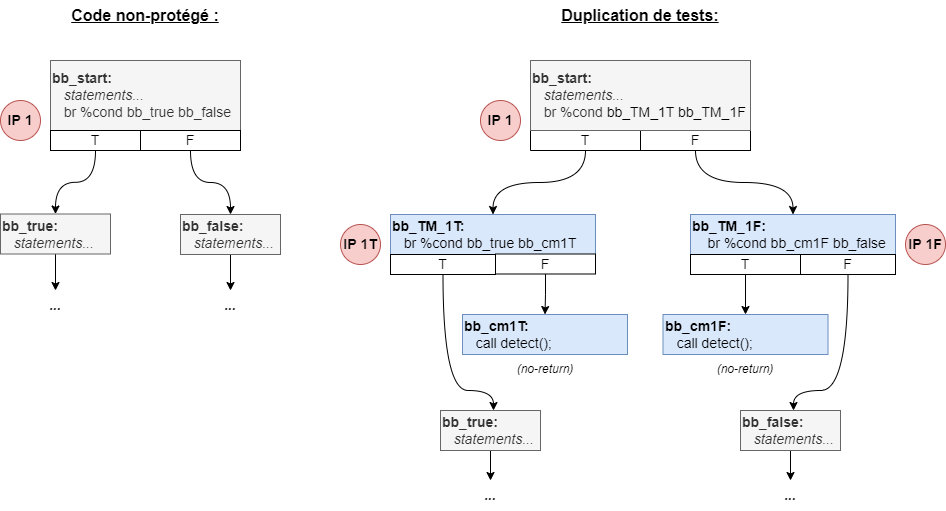
\includegraphics[scale=0.4]{ch5-placement/img/cm-mul-test-large-simple.drawio.png}
                    \caption{Schéma de protection de la duplication de test}
                    \label{fig:td-scheme}
                \end{figure}
                
                \begin{defi}
                    \label{def:cm-application}
                    Soit $P$ un programme et $C$ une contre-mesure, on note $C(P)$ l'application de $C$ sur $P$.
                \end{defi}
                \begin{defi}
                    \label{def:cm-application-local}
                    Soit $C$ une contre-mesure à granularité d'un point d'injection, on note $C(P, IP)$ l'application de $C$ localement sur le point d'injection $IP$.
                \end{defi}
                
                \begin{defi}
                    \label{def:cm-independance}
                    On dit que deux contre-mesures $C_1$ et $C_2$ sont indépendantes (noté $\perp$) ssi, pour tout programme $P$, leur ordre d'application n'a pas d'incidence\footnote{En d'autres termes, les programmes obtenus sont syntaxiquement équivalents quel que soit l'ordre d'application des contre-mesures.} sur le programme protégé obtenu :
                    $C_1 \perp C_2 \leftrightarrow C_2(C_1(P)) = C_1(C_2(P))$.
                \end{defi}
                
                \begin{defi}
                    \label{def:cm-local}
                    Pour un modèle de faute $m$, une contre-mesure $C$ est dite \textit{locale}, ssi, pour tout programme $P$, toutes les applications de C pour chaque point d'injection sont indépendantes: $\forall IP_a, IP_b \in IP(P), C(P, IP_a) \perp C(P, IP_b)$.
                \end{defi}
                
                \gls{TD} est une contre-mesure locale (définition \ref{def:cm-local}), puisqu'elle s'applique sur les points d'injection d'inversion de test (granularité \gls{ip}) et chaque application est indépendante (définition \ref{def:cm-independance}).
                Cette notion de \textit{localité} est importante pour le placement de contre-mesures, puisque dans le cas de contre-mesures locales, il est possible de représenter l'application de la contre-mesure comme un ensemble non ordonné de points d'injection.
                
            \subsubsection{Contre-mesures locales pondérées}
            \label{sec:cm-ponderated}
    
                La multiplication de tests est un exemple de contre-mesure locale pouvant être appliquée avec un niveau de pondération différent pour chaque point d'injection.
                On parle alors de \gls{CLP}, et on appelle \textit{profondeur} le coefficient d'application d'une contre-mesure pour un point d'injection donné (définition \ref{def:cm-ponderated}).
                
                \begin{figure}[p]\centering
                    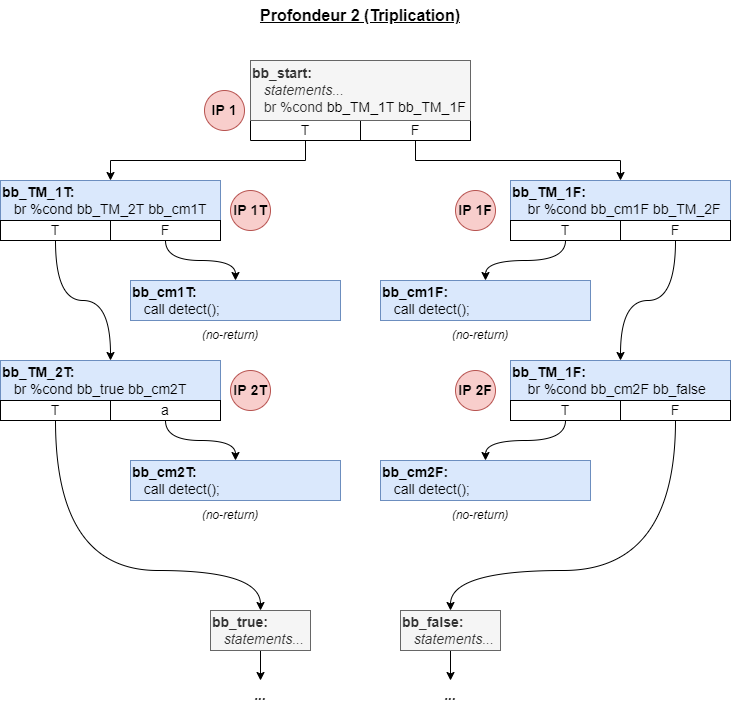
\includegraphics[scale=0.45]{ch5-placement/img/cm-mul-tripl.png}
                    \caption{Schéma de protection de la triplication de test}
                    \label{fig:tt-scheme}
                \end{figure}
            
                \begin{figure}[p]\centering
                    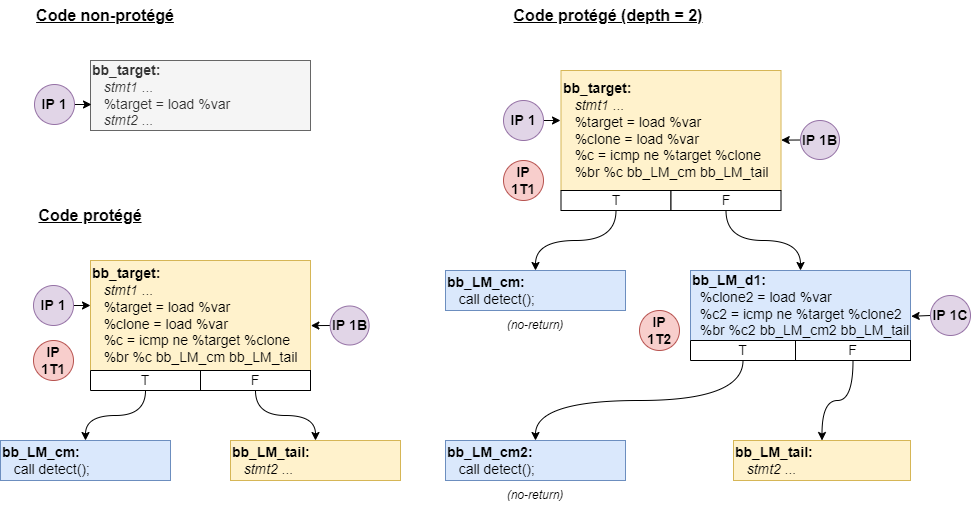
\includegraphics[scale=0.39]{ch5-placement/img/cm-mul-load-full-sep.drawio.png}
                    \caption{Schéma de protection de la multiplication de load}
                    \label{fig:lm-scheme}
                \end{figure}
            
                \begin{defi}
                    \label{def:cm-ponderated}
                    Une contre-mesure locale est dite \textit{pondérée} s'il est possible de l'appliquer avec une profondeur $p$ positive.
                    On note $C_p(P, IP)$ l'application d'une contre-mesure locale pondérée $C$ sur un point d'injection $IP$ avec une profondeur $p \in \mathbb{N}$.
                \end{defi}
                
                Ainsi, la \textit{duplication de test} correspond à une \textit{multiplication de test} de profondeur $1$.
                La figure \ref{fig:tt-scheme} présente le schéma de transformation de la multiplication de tests pour une profondeur $2$ (\gls{TT}). 
                Les points d'injection sont indiqués dans les cercles rouges à côté de l'instruction de branchement correspondante.
                La multiplication de tests peut être vue comme l'application successive de duplications de tests sur les points d'injection introduits par l'itération précédente, en ignorant la protection des branches allant vers un bloc de détection (c'est-à-dire contenant un appel à \textit{detect()} dans les schémas de protection présentés).        
                
                Les contre-mesures locales pondérées peuvent être appliquées avec une profondeur variable sur chaque point d'injection.
                L'intérêt de tels schémas dépend du fait qu'une application de profondeur $n+1$ apporte plus de garanties de sécurité qu'une application de profondeur $n$, pour un modèle de faute $m$, ce qu'on va pouvoir quantifier dans la suite de ce chapitre.
            
            \subsubsection{Multiplication de loads}
            \label{sec:cm-load-mult}
            
                La multiplication de tests vise le modèle de l'inversion de test (\gls{TI}). La multiplication de loads (\gls{LM}) est une contre-mesure locale pondérée visant le modèle de la mutation de données lors les \textit{loads} (\gls{DL}).
                
                La figure \ref{fig:lm-scheme} présente le schéma de protection de la multiplication de loads avec une profondeur $0$ (code non protégé), $1$ (\gls{LD}) et $2$ (\gls{LT}).
                Les points d'injection en rouge correspondent au modèle de faute \gls{TI} tandis que les violets correspondent au modèle \gls{DL}.
                Les blocs de base en jaune indiquent des blocs comportant à la fois des instructions du programme original et du code de contre-mesure.
                Dans le cas de la protection de profondeur 1, l'instruction \texttt{load} est dupliquée et les deux valeurs sont comparées. Si celles-ci sont différentes, le programme est arrêté, sinon le flot de contrôle revient à l'instruction suivant le \texttt{load} ciblé (ici dans un nouveau bloc \texttt{bb\_LM\_tail}). 
                Dans le cas de protection de profondeur 2 ou plus, comme indiqué dans la partie droite de la figure, les \texttt{load}s dupliqués sont comparés à la valeur du \texttt{load} original, générant ainsi plusieurs branchements conditionnels successifs.
            
        \subsection{Adéquation et coefficient de protection}
        \label{sec:cm-perfection}
        
            Cette section s'intéresse à la propriété d'adéquation d'une contre-mesure, définie par rapport à un modèle de faute.
            Cette propriété est nécessaire pour établir des garanties de robustesse pour les différents algorithmes de placement.
            La section \ref{sec:ooc} présente une approche d'analyse de contre-mesures \textit{en isolation}, visant à étudier les propriétés du schéma de protection en dehors d'un programme particulier.
            La section \ref{sec:fscenario} détaille le cas d'une analyse dans le scénario où une entrée est déjà corrompue.
            La section \ref{sec:cm-perfect} définit l'adéquation d'une contre-mesure locale à l'aide de cette analyse.
            
            \subsubsection{Analyse en isolation de schémas de protection}
            \label{sec:ooc}
            
                L'approche présentée ici consiste à s'intéresser aux comportements d'un schéma de protection en isolation, relativement à un modèle de faute.
                L'idée est d'explorer tous les chemins d'exécution fautée en prenant pour entrée le point d'injection (ici une instruction \gls{llvm}) en fonction du modèle de faute $m$ 
                afin de déterminer le nombre de fautes nécessaires pour le corrompre, appelé \textit{coefficient de protection} (définition \ref{def:cm-k}).
                Puisqu'un point d'injection est par définition attaquable en une faute, un schéma de protection avec $K > 1$ apporte des garanties sur la robustesse du schéma de protection.
                
                \begin{defi}
                    \label{def:cm-k}
                    Soit $S$ un schéma de protection sur un point d'injection, on appelle \textit{coefficient de protection} $K$ le nombre minimum de fautes nécessaires pour produire un comportement incorrect, pour un modèle de faute donné.
                \end{defi}     
                
                L'analyse en isolation d'un schéma de protection pour un modèle de faute $m$ nécessite de déterminer :
                \begin{itemize}
                    \item Les \textit{points d'entrée} et les \textit{points de sortie} du schéma de protection.
                    \item Les \textit{entrées} du schéma de protection.
                    \item Les \textit{sorties} du schéma de protection.
                    \item La \textit{surface d'attaque} du schéma de protection par rapport au modèle $m$.
                \end{itemize}

                \paragraph{}
                \textbf{Points d'entrée et de sortie.} Les \textit{points d'entrée et de sortie} sont définis par le schéma de protection, mais également par le modèle de faute $m$. Pour un modèle de faute de saut par exemple, l'exploration exhaustive des comportements du schéma de protection nécessite de prendre en compte comme points d'entrée chaque point d'arrivée de saut possible et comme points de sortie les points d'injection de saut.
                Les schémas de \gls{LM} et \gls{TM} (voir figure \ref{fig:td-scheme}, \ref{fig:tt-scheme} et \ref{fig:lm-scheme}) ne contiennent qu'un seul point d'entrée correspondant à l'instruction sur laquelle le schéma de protection s'applique (respectivement \texttt{br} et \texttt{load}).
                Le schéma \gls{LM} n'a qu'un seul point de sortie (le bloc \texttt{bb\_LM\_tail}) tandis que \gls{TM} en possède deux (les blocs cibles \texttt{bb\_true} et \texttt{bb\_false}).
                Notez qu'on ne considère pas les blocs de détection comme des points de sorties.
                
                \textbf{Entrées.} Les \textit{entrées} correspondent à tout état du programme qui est utilisé par le schéma de protection. Dans le cadre de la contre-mesure \gls{TM}, l'unique entrée est la valeur de condition \texttt{\%cond}, utilisée par les instructions de branchement.
                Pour la contre-mesure \gls{LM}, l'unique entrée est la valeur de la variable lue par les instructions \texttt{load}.
                
                \textbf{Sorties.} Les \textit{sorties} correspondent aux états du programme qui sont susceptibles d'être modifiés par le schéma de protection.
                Pour \gls{TM}, il s'agit du bloc d'arrivée ($bb\_true$ ou $bb\_false$). Pour \gls{LM}, la sortie correspond à la valeur lue par l'instruction \texttt{load}\footnote{C'est à dire la valeur qui sera stockée dans le registre temporaire \gls{llvm} $\%target$.}. 
                Les sorties sont nécessaires pour déterminer l'objectif d'attaque de l'analyse en isolation, une attaque réussie du schéma \gls{TM} correspondant à un branchement vers la mauvaise branche en sortie et pour \gls{LM} au chargement de la mauvaise valeur lors du load (sans qu'aucune fonction \texttt{detect} ne soit déclenchée).
                Il est possible d'avoir plusieurs sorties si on considère des contre-mesures avec \textit{état}, telles que \textit{SecSwift CF} \cite{Ferriere/LLVM19} citée précédemment.
                
                \textbf{Surface d'attaque.} La \textit{surface d'attaque} du schéma de protection correspond à tous les points d'injection du modèle $m$, que ce soit le point d'injection nominal (celui sur lequel le schéma s'applique) mais aussi les points d'injection introduits par la contre-mesure.
                
                \begin{defi}[Surface d'attaque]
                    \label{def:cm-ips}
                    Soit $C$ une contre-mesure et $IP$ un point d'injection, on note $IPs(C(P, IP))$ l'ensemble des points d'injection introduits par l'application $C(P, IP)$.
                \end{defi}
                    
                \begin{figure}[p]\centering
            \begin{multicols}{2} 

\lstset{language=C,style=codeC, caption={Encodage de $TD$ ($TM_1$)},label={lst:td-scheme-lazart}, showlines=true}
\begin{lstlisting}
int tm_scheme(int cond) {
    bb_start:
    if(cond) {
        bb_TM_1T:
        if(cond) {
            bb_true:
            return true;
        } else {
            bb_cm1T:
            detect();
        }
    } else {
        bb_TM_1F:
        if(cond) {
            bb_cm1F:
            detect();
        } else {
            bb_false:
            return false;
        }
    }
}













\end{lstlisting}  
\columnbreak

\lstset{language=C,style=codeC, caption={Encodage de $TT$ ($TM_2$)},label={lst-tt-scheme-lazart}, showlines=true}
\begin{lstlisting}
int tm_scheme(int cond) {
    bb_start:
    if(cond) {
        bb_TM_1T:
        if(cond) {
            bb_TM_2T:
            if(cond) {
                bb_true:
                return true;
            } else {
                bb_cm2T:
                detect();
            }
        } else {
            bb_cm1T:
            detect();
        }
    } else {
        bb_TM_1F:
        if(cond) {
            bb_cm1F:
            detect();
        } else {
            bb_TM_2T:
            if(cond) {
                bb_cm2F:
                detect();
            } else {
                bb_false:
                return false;
            }
        }
    }
}

\end{lstlisting} 
\end{multicols}
            \end{figure}

\begin{figure}[p]\centering
\lstset{caption={Fonction principale de l'analyse en isolation (scénario nominal)},label=lst:ooc-main-lazart}
\begin{lstlisting}
int main() {
    int entry;
    klee_make_symbolic(&entry, sizeof(entry), "cond");

    int br = tm_scheme(entry);

    _LZ__ORACLE((br != (entry ? true : false)));
}
\end{lstlisting}
            \end{figure}
        
                A partir de ces quatre paramètres, il est possible d'explorer les exécutions fautées du schéma de protection. Cette exploration peut être effectuée avec Lazart\footnote{Le nombre de chemins à explorer dans une analyse en isolation est généralement petit. Ainsi, il est possible de vérifier manuellement que l'exploration symbolique est correcte et complète.}, comme montré dans les listings \ref{lst:td-scheme-lazart} et \ref{lst-tt-scheme-lazart} qui correspondent à l'encodage en langage C des schémas de protection de la multiplication de tests, respectivement pour une profondeur de $1$ et de $2$.
                Les noms des blocs de base (correspondant à ceux des figures \ref{fig:td-scheme} et \ref{fig:tt-scheme}) sont indiqués en tant qu'étiquettes (labels ).
                L'entrée du schéma de protection est représentée par l'entier \texttt{cond} et la branche de sortie est représentée sous la forme d'un booléen (branche \textit{true} ou branche \textit{false}).
                Les appels à \texttt{detect()} correspondent à une détection de l'attaque.
        
                Le listing  \ref{lst:ooc-main-lazart} correspond à la fonction principale de l'analyse avec Lazart.
                La condition d'entrée est déclarée comme variable symbolique (ligne 3) et l'objectif d'attaque consiste à retourner la mauvaise branche (vérifié ligne 7).
                La recherche des chemins d'attaque est effectuée en fautant la fonction correspondant au schéma de protection (ici \texttt{tm\_scheme}) avec le modèle $m$ (ici \gls{TI}).

                La table \ref{tbl:tm-ooc-N} présente les résultats de l'analyse en isolation pour différentes profondeurs de protection de la multiplication de tests.
                La colonne "Contre-mesure" indique le schéma de protection: $P$ correspondant à une profondeur 0 (code non protégé), \gls{TD} à la duplication de test (\gls{TM} profondeur 1) et \gls{TT} à la triplication de test (\gls{TM} de profondeur 2).
                Les colonnes suivantes indiquent le nombre d'attaques trouvées pour chaque nombre de fautes et la dernière colonne "$K_n$" correspond au \textit{coefficient de protection nominal}, c'est-à-dire le nombre minimum de fautes nécessaires pour valider l'objectif d'attaque.
    
                \begin{table}[ht]
                    {\small
                    \begin{center}
                        \begin{tabular}{l|cccccc}
                        Contre-mesure & 0 faute & 1 faute & 2 fautes & 3 fautes & 4 fautes & $K_n$ \\
                        \hline
                        $TM_0$ ($P$) & 0 & 1 & 0 & 0 & 0 & 1\\
                        $TM_1$ ($TD$) & 0 & 0 & 1 & 0 & 0 & 2 \\
                        $TM_2$ ($TT$) & 0 & 0 & 0 & 1 & 0 & 3
                        \end{tabular}
                    \end{center} 
                    }
                    \caption{Évaluation en isolation de $TM$ \label{tbl:tm-ooc-N}}
                \end{table}
            
            \subsubsection{Scénario corrompu}
            \label{sec:fscenario}
            
                Afin d'être exhaustif sur l'exploration des comportements, il est nécessaire de se pencher sur le cas où les entrées de la contre-mesure sont déjà corrompues (par une faute précédente).
                Ainsi, la méthodologie d'analyse en isolation distingue deux scénarios, comme indiqué dans la figure \ref{fig:out-of-context}:
                \begin{itemize}
                    \item Scénario Nominal (N) : toutes les entrées sont saines (traité dans la section précédente).
                    \item Scénario Corrompu (C) : une entrée au moins est corrompue en amont du schéma de protection.
                \end{itemize}
                
                \begin{table}[ht]
                    {\small
                    \begin{center}
                        \begin{tabular}{l|cccccc}
                        Contre-mesure & 0 faute & 1 faute & 2 fautes & 3 fautes & 4 fautes & $K_c$ \\
                        \hline
                        $TM_0$ ($P$) & 1 & 0 & 0 & 0 & 0 & 0\\
                        $TM_1$ ($TD$) & 1 & 0 & 0 & 0 & 0 & 0\\
                        $TM_2$ ($TT$) & 1 & 0 & 0 & 0 & 0 & 0
                        \end{tabular}
                    \end{center} 
                    }
                    \caption{Évaluation en isolation de $TM$ (scénario corrompu)\label{tbl:tm-ooc-F}}
                \end{table}
                      
                \begin{figure}[!htp]\centering
                    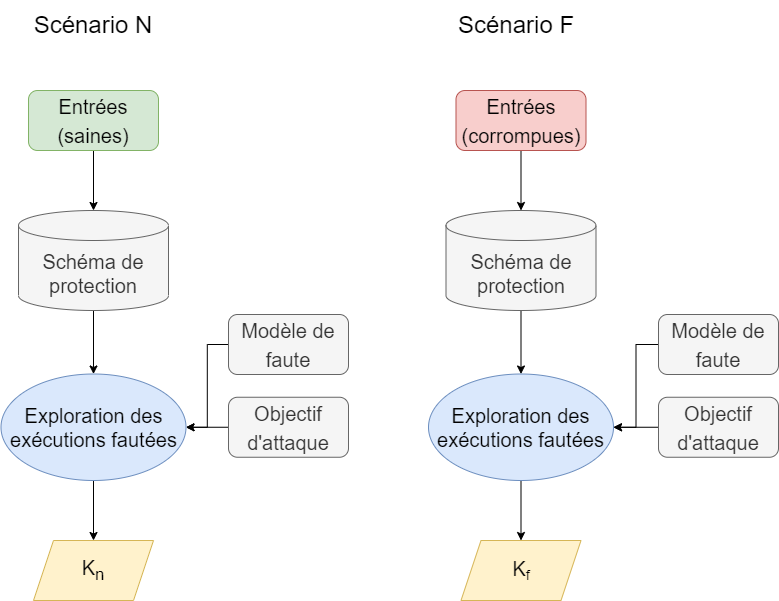
\includegraphics[scale=0.39]{ch5-placement/img/out-of-context-metho.png}
                    \caption{Évaluation de schéma de protection en isolation}
                    \label{fig:out-of-context}
                \end{figure}
        
                La table \ref{tbl:tm-ooc-F} présente les résultats (après analyse de redondance-équivalence) du scénario corrompu (C) pour l'exemple précédent, la condition d'entrée étant falsifiée (en changeant donc l'appel ligne 5 en \texttt{int br = tm\_scheme(!entry);}\footnote{Dans le cas d'une entrée non booléenne, celle-ci serait contrainte comme étant différente de la valeur nominale (\texttt{\_LZ\_\_ORACLE(entry != expected\_value);}.}). 
                On appellera respectivement \textit{coefficient de protection nominal} ($K_n$) et \textit{coefficient de protection corrompu} ($K_c$) les coefficients de protection obtenus pour respectivement les scénarios $N$ et $C$.
                Pour les contre-mesures \gls{TM} et \gls{LM} et leurs modèles de faute respectifs \gls{TI} et \gls{DL} avec une pondération d'application $p$, on obtient $K_n = 1 + p$ et $K_c = 0$. 
                Cela implique que, si les entrées d'un schéma de protection \gls{TM} ou \gls{LM} sont nominales, alors on a la garantie que le programme sera dans un état nominal en sortie du schéma de protection en moins de $1 + p$ fautes injectées localement. 
                En revanche, dans le scénario corrompu, tous les schémas de protection produisent un comportement incorrect même en l'absence de faute, de la même manière que le point d'injection non protégé.
                
            \subsubsection{Adéquation des contre-mesures}
            \label{sec:cm-perfect}
        
                \begin{defi}[Adéquation]
                    \label{def:cm-pperfect}
                    Pour un modèle de faute $m$, une contre-mesure locale $C$ est dite \textit{adaptée} ssi, pour tout programme $P$, son coefficient de protection nominal $K_n$ est strictement supérieur à 1.
                \end{defi}
                
                \begin{defi}[Perfection]
                    \label{def:cm-perfect}
                    Pour un modèle de faute $m$, une contre-mesure locale $C$ est dite \textit{parfaite} ssi, pour tout programme $P$, son coefficient de protection $K = min(K_n, K_c)$ est strictement positif. 
                \end{defi}
                
                Une contre-mesure parfaite (définition \ref{def:cm-perfect}) garantit que, quelles que soient les entrées d'une contre-mesure, tout état invalide du programme sera détecté. 
                La section \ref{sec:model-protectability} revient sur l'existence de telles contre-mesures, mais on peut observer que ce n'est pas le cas des contre-mesures \gls{TM} et \gls{LM}, qui ont $K_c$ nul. En effet, si les entrées sont déjà corrompues, alors le comportement du point d'injection protégé restera incorrect (mauvaise branche ou valeur incorrecte) sans qu'aucune faute ne soit injectée.
                En revanche, \gls{TM} et \gls{LM} sont des contre-mesures adaptées (définition \ref{def:cm-pperfect}) pour respectivement les modèles \gls{TI} et \gls{DL} (propriétés \ref{hypo:test-mult} et \ref{hypo:load-mult}).
                Comme cela a été expliqué dans la section précédente, l'analyse en isolation avec l'exécution symbolique (via Lazart) génère peu de chemins pour nos exemples et il est donc possible de vérifier la complétude de l'exploration des chemins manuellement. 
                La preuve de la propriété d'adéquation d'un schéma de protection par rapport à un modèle de faute pourrait aussi être effectuée à l'aide d'un outil d'analyse statique ou d'un assistant de preuve.
                
                \begin{proper}
                    \label{hypo:test-mult}
                    La multiplication de tests est une contre-mesure locale pondérée adaptée pour le modèle de l'inversion de test (\gls{TI}).
                \end{proper}
            
                \begin{proper}
                    \label{hypo:load-mult}
                    La multiplication de loads est une contre-mesure locale pondérée adaptée pour le modèle de la mutation de données sur les loads (\gls{DL}).
                \end{proper}
                
        \subsection{Complétude d'une contre-mesure et catalogue}
        \label{sec:cm-complete}
         
            Les contres-mesures \gls{TM} et \gls{LM} sont chacune des contres-mesures adaptées pour respectivement les modèles \gls{TI} et \gls{DL}. 
            \gls{TM} et \gls{LM} sont aussi adaptées pour le modèle combiné de l'inversion de test et de la mutation de données ($TI+DL$).
            En effet, chacune a un coefficient de protection nominal $K_n$ strictement supérieur à 1 lorsqu'on les étudie en fonction du modèle $m = TI+DL$.
            
            Néanmoins, ni \gls{TM}, ni \gls{LM}, ne permettent indépendamment la protection de l'ensemble des points d'injection du modèle $TI+DL$. On dit alors que chacune de ces contre-mesures sont \textit{incomplètes} pour le modèle $TI+DL$ (définition \ref{def:cm-compl}).
            Ainsi, on appellera \gls{TLM} la contre-mesure locale pondérée correspondant à l'application de \gls{TM} sur les points d'injection \gls{TI} et \gls{LM} pour les points d'injection \gls{DL}. Cette contre-mesure est complète et adaptée pour le modèle $TI+DL$ (propriété \ref{hypo:tl-mult}).
            
            \begin{defi}
                \label{def:cm-compl}
                Une contre-mesure locale est dite \textit{complète} pour un modèle de faute $m$, si elle propose une schéma de protection pour tous les points d'injection générés par le modèle de faute $m$.
            \end{defi}
        
            \begin{proper}
                \label{hypo:tl-mult}
                La multiplication de tests et de loads (\gls{TLM}) est une contre-mesure locale pondérée adaptée et complète pour le modèle $TI+DL$.
            \end{proper}

            Les algorithmes de placement qui seront présentés par la suite considèrent un \textit{catalogue} de contre-mesures.
            Ce catalogue associe un schéma de protection en fonction d'un point d'injection suivant son modèle de faute et un coefficient de protection.
            \gls{TLM} peut être vu comme un catalogue de contre-mesure associant \gls{TM} aux points d'injection \gls{TI} et \gls{LM} aux points d'injections \gls{DL}, le schéma de protection précis qui sera retourné dépendant du coefficient de protection demandé\footnote{Par exemple, pour un point d'injection \gls{TI} et un coefficient de protection de $2$, le catalogue retournerait la duplication de test.}.            
            Les notions d'adéquation et de complétude peuvent être étendues à un catalogue de contre-mesures (définitions \ref{def:catalog-adatp} et \ref{def:catalog-complete}).
            Les algorithmes de placement présentés par la suite considèrent les catalogues totaux\footnote{Un catalogue total est complet et adapté.} (définition \ref{def:catalog-pond-adatp}).
            
            \begin{defi}[Catalogue adapté]
                \label{def:catalog-adatp}
                Un catalogue de contre-mesures $\mathcal{C}$ est adapté pour un modèle de faute $m$, si toutes les schémas de protection sont adaptés pour le modèle $m$.
            \end{defi}
            
            \begin{defi}[Catalogue complet]
                \label{def:catalog-complete}
                Un catalogue de contre-mesures $\mathcal{C}$ est complet pour un modèle de faute $m$, s'il associe un schéma de protection pour tous les points d'injection du modèle de faute $m$.
            \end{defi}
            
            \begin{defi}[Catalogue total]
                \label{def:catalog-pond-adatp}
                Un catalogue de contre-mesures $\mathcal{C}$ est dit total pour un modèle de faute $m$, s'il possède un schéma de protection pour tout points d'injection et pour tout coefficient de protection $k$, avec $1 \leq k \leq n+1$, pour $m$, avec $n \in \mathbb{N}^*$.
            \end{defi}

            Un catalogue de contre-mesures n'est donc finalement qu'une forme particulière de contre-mesure, permettant de garantir qu'un point d'injection est protégé qu'une fois par un schéma de protection (quelle que soit la profondeur d'application choisie).
            De cette manière, plusieurs contre-mesures (de l'ordre du point d'injection) qui ne sont pas indépendantes peuvent être appliquées de manière indépendante.
            En effet, les contre-mesures \gls{TM} et \gls{LM} ne sont pas indépendantes. \gls{LM} introduit des points d'injections \gls{TI} qui peuvent ainsi être protégés par une application de \gls{TM} (en d'autres termes, $TM(LM(P)) \neq LM(TM(P))$).
            Il est donc nécessaire de s'assurer qu'un point d'injection ne soit pas protégé plusieurs fois de manière à garantir l'indépendance de l'application.
                    
        \subsection{Synthèse}
        \label{sec:cm-synthesis}
        
            La table \ref{tbl:local-cm-comparison} présente un résumé des caractéristiques des différentes contre-mesures abordées dans cette section. La colonne "CM" indique le nom de la contre-mesure.
            Les colonnes "Adéquation" et "Complétude" indiquent respectivement si la contre-mesure est adaptée et complète, par rapport aux différents modèles de faute. Pour la complétude, la valeur "-" indique que la contre-mesure ne permet de protéger aucun point d'injection du modèle de faute.
            La colonne "Surface d'attaque" indique le nombre de points d'injection générés par la contre-mesure pour une profondeur $p$ respectivement pour les modèles \gls{TI} et \gls{DL} (c'est-à-dire $IPs(C_p(P, IP))$).
            Ces valeurs ne sont pas indiquées pour \gls{TLM} puisqu'elle correspond à celles de \gls{TM} ou \gls{LM} en fonction du modèle du point d'injection protégé.
            
            \begin{table}[h]
                {\small
                \begin{center}
                    \begin{tabular}{c|ccc|ccc|cc}
                    CM & \multicolumn{3}{c|}{Adéquation} & \multicolumn{3}{c|}{Complétude} & \multicolumn{2}{c}{Surface d'attaque}  \\
                    \multicolumn{1}{l|}{} & TI & DL & TI+DL & TI & DL & TI+DL & TI & DL  \\
                    \hline
                    \gls{TM} & Oui & Oui & Non & Oui & - & Non & $2p$ & $0$  \\
                    \gls{LM} & Oui & Oui & Non & - & Oui & Non & $p$ & $1 + p$ \\
                    \gls{TLM} & Oui & Oui & Oui & Oui & Oui & Oui & - & - 
                    \end{tabular}
                \end{center} 
                }
                \caption{Comparaison des contre-mesures locales pondérées\label{tbl:local-cm-comparison}}
            \end{table}
        
            Les notions de contre-mesures \textit{locales} et \textit{pondérées} sont nécessaires pour les algorithmes de placement.
            Ces contre-mesures peuvent être représentées par l'ensemble des pondérations associées à chaque point d'injection de fautes du programme, une pondération de 0 correspondant à ne pas protéger le point d'injection. 
            Si on considère des contre-mesures locales mais non pondérées (\gls{CL}), leur application est aussi un ensemble de pondérations dont les valeurs sont comprises entre 0 et 1.
            Enfin, dans le cas de contre-mesures à granularité du point d'injection mais non indépendantes (C), alors l'ordre dans lequel les protections sont appliquées est important. Dans ce cas, l'application de la contre-mesure peut être représentée par une liste ordonnée de points d'injection à protéger.
            Les notions d'\textit{adéquation} et de \textit{complétude} sont quant à elles utiles pour déterminer les garanties en terme de robustesse pour un algorithme de placement. 
            
            \begin{table}[htp]
                {
                \begin{center}
                    \begin{tabular}{l|cc}
                    Contre-mesure & Acronyme & Autre nom \\
                    \hline 
                    Multiplication de tests & $TM$ & - \\
                    $\;\;$ Duplication de tests & $\;TD$ & $\;TM_1$ \\
                    $\;\;$ Triplication de tests & $\;TT$ & $\;TM_2$ \\
                    Multiplication de loads & $LM$ & - \\
                    $\;\;$ Duplication de loads & $\;LD$ & $\;LM_1$ \\
                    $\;\;$ Triplication de loads & $\;LT$ & $\;LM_2$ \\
                    \begin{tabular}[c]{@{}l@{}}Multiplication de loads\\ et de tests\end{tabular} & $TLM$ & -
                    \end{tabular}
                \end{center} 
                }
                \caption{Abréviation pour les différentes contre-mesures locales de Lazart\label{tbl:cm:nomenclature}}
            \end{table}
            
            \begin{table}[htp]
                {\small
                \begin{center}
                    \setlength\tabcolsep{5pt}
                    \begin{tabular}{l|cccc}
                    Localité / Pondération & \multicolumn{4}{c}{Adéquation / Complétude} \\
                     & Inadaptée (-I) & Adaptée (-A) & Complète (-C) & Parfaite (-P) \\
                     \hline
                    CM non locale (C) & C-I & C-A & C-C & C-P \\
                    CM Locale (CL) & CL-I & CL-A & CL-C & CL-P \\
                    CM Locale Pondérée (CLP) & CLP-I & CLP-A & CLP-C & CLP-P
                    \end{tabular}
                \end{center} 
                }
                \caption{Abréviation pour les différentes catégories de contre-mesures à granularité IP\label{tbl:cm:nomenclature-types}}
            \end{table}
        
            Les tables \ref{tbl:cm:nomenclature} et \ref{tbl:cm:nomenclature-types} proposent un résumé des abréviations qui seront utilisées dans la suite de ce chapitre. La table \ref{tbl:cm:nomenclature} indique les abréviations utilisées pour les contre-mesures étudiées ici. La table \ref{tbl:cm:nomenclature-types} indique les abréviations concernant les différentes classes de contre-mesures. Par exemple, \gls{CLP}-AC correspond à une Contre-mesure Locale Pondérée, Adaptée et Complète (pour un modèle de faute donné).
            
    \section{Placement de contre-mesures adaptées}
    \label{sec:placement}

        L'approche de placement de contre-mesures présentée dans ce chapitre se base sur l'analyse en isolation des schémas de protections et sur une exploration des traces d'attaques réussies, par rapport à un modèle de faute et un objectif d'attaque.
        L'analyse en isolation fournit des garanties sur le comportement d'un point d'injection protégé, et les traces d'attaques permettent de déterminer quels sont les points d'injection à protéger.
        Les algorithmes présentés ici prennent ainsi en entrées:
        \begin{itemize}
            \item Le catalogue de contre-mesures $\mathcal{C}$.
            \item Le modèle d'attaquant $M = \{m, \phi\}$, avec $m$ le modèle de faute et $\phi$ l'objectif d'attaque.
            \item Le nombre de fautes $n$ pour lequel on souhaite être robuste.
        \end{itemize}

        Le catalogue $\mathcal{C}$ est un catalogue total (définition \ref{def:catalog-pond-adatp}) pour le modèle $m$.
        Les garanties de robustesse sont données en supposant que l'énumération des chemins d'attaque est \textit{correcte} et \textit{complète} (définitions \ref{def:fi-sound} et \ref{def:fi-complete}).
        Les algorithmes génèrent un programme $P'$ protégé dont les garanties dépendent de l'algorithme et du catalogue, et visent:
        \begin{itemize}
            \item La \textit{robustesse} du programme $P'$ en $n$ fautes.
            \item L'\textit{optimalité} du placement.
        \end{itemize}

        La section \ref{sec:placement-syst} présente trois algorithmes de placement systématique.
        La section \ref{sec:placement-bloc} décrit le placement par bloc, dans lequel seul un \gls{ip} par trace d'attaque est protégé.
        La section \ref{sec:placement-opti} traite du placement réparti où différents \gls{ip}s peuvent être protégés avec des coefficients de protection différents.
        Finalement, la section \ref{sec:placement-other} discute des garanties lorsque le catalogue ne dispose pas d'un schéma avec un coefficient de protection suffisant et discute de certaines variantes des algorithmes précédents.  
            
        \subsection{Placement systématique}
        \label{sec:placement-syst}

            Lorsqu'on s'intéresse à un catalogue total pour le modèle de faute $m$, appliquer un schéma de protection avec un coefficient de protection nominal $K_n = n+1$ sur tous les points d'injection garantit une robustesse en au moins $n$ fautes du programme protégé. 
            En effet, l'analyse en isolation garantit que le comportement du schéma de protection est nominal en moins de $n + 1$ fautes si les entrées sont nominales. Si tous les points d'injection sont protégés avec $K_n = n+1$, il faudra $n + 1$ fautes pour casser indépendamment chaque schéma et aucun schéma de protection ne pourra être corrompu en $n$ fautes.

            On distinguera trois versions de l'algorithme de placement systématique:
            \begin{itemize}
                \item Le placement systématique naïf (\texttt{naïf}): tous les points d'injection du programme sont protégés avec $K_n = n+1$.
                \item Le placement systématique sur les attaques (\texttt{atk}): tous les points d'injection intervenant au moins une fois dans une attaque sont protégés avec $K_n = n+1$.
                \item Le placement systématique sur les minimales (\texttt{min}): seuls les points d'injection intervenant dans les attaques minimales sont protégés avec $K_n = n+1$.
            \end{itemize}

            Si l'énumération des chemins fautés est correcte et complète, alors protéger les points d'injection intervenant dans les attaques est suffisant.
            De plus, la protection des attaques minimales est suffisante, puisque si une attaque $a'$ est redondante par rapport à une attaque $a$, protéger $a$ pour $n$ fautes implique que $a'$ sera robuste en $n+1$ fautes au minimum.

            Le listing \ref{lst:placement-syst} correspond au pseudo-code de l'algorithme de placement systématique sur les attaques minimales (\texttt{min}) prenant en entrées le catalogue $\mathcal{C}$, le programme $P$, le modèle d'attaquant $M$ et le nombre de fautes $n$ pour lequel le programme $P'$ doit être robuste.
            Les attaques minimales sont obtenues à partir d'une analyse d'attaque et une analyse de redondance (lignes 3 et 5) puis chaque point d'injection intervenant au moins une fois dans une attaque minimale se voit assigner un coefficient de protection de $n + 1$ (lignes 11 à 13).
            Le programme $P'$ est généré à partir de l'ensemble des coefficients de protection (lignes 16 à 19) en sélectionnant le schéma de protection à appliquer à partir du catalogue (représenté par la fonction \texttt{get\_cm} ligne 18).

\lstset{caption={Algorithme de placement systématique \texttt{min}},label=lst:placement-syst, showlines=true}
\begin{lstlisting}
def placement_min(C: Catalog, P: Program, M: AttackModel, n: int):
    # Get sucessfull non-detected attacks.
    attacks = T_s(P, M, n)
    # Filter with minimals attacks.
    minimals = RedundacyAnalysis(attacks).minimals()
    
    # Initial protection factors Kn at 1 for all IP.
    required_kn = { IPA: 1, IPB: 1, ..., IPN: 1 }

    # Apply ponderation of n for all IP in traces
    for attack in minimals:
        for IP in attack:
            required_kn[IP] = n + 1 # Make IP robust en n faults.

    # Generation of P'
    P` = P
    for IP, kn in required_kn:
        S = C.get_cm(IP.model(), kn) # Select protection scheme from catalog
        P` = S(P`, IP) # Apply local protection        
    return P`
\end{lstlisting}  

        \subsection{Placement par bloc}
        \label{sec:placement-bloc}

            L'algorithme de placement systématique sur les attaques minimales protège l'ensemble des points d'injection intervenant dans une attaque.
            L'algorithme de placement par bloc (\texttt{bloc-h}) présenté dans cette section vise à protéger au moins un point d'injection par attaque minimale, avec $K_n = n + 1$.

\lstset{caption={Algorithme de placement par bloc avec heuristique \texttt{bloc-h}},label=lst:placement-bloc-h, showlines=true}
\begin{lstlisting}
def placement_bloc_h(C: Catalog, P: Program, M: AttackModel, n: int):
    # Get sucessfull non-detected attacks.
    attacks = T_s(P, M, n)
    # Filter with minimals attacks.
    minimals = RedundacyAnalysis(attacks).minimals()
    
    # Initial protection factors Kn at 1 for all IP.
    required_kn = { IPA: 1, IPB: 1, ..., IPN: 1 }
            
    # For all attacks by faults count.
    for order in 1 to n:
        # Loop trought order-faults attacks by number of associated redundant attacks.
        for attack in minimals.where(order=order).sort_by(Minimals):
            if is_protected(attack, required_kn):
                continue
            # Make attack robust in n faults
            IP = select IP in attack with most occurence
            required_kn[IP] = n

    # Generation of P'
    P` = P
    for IP, kn in required_kn:
        S = C.get_cm(IP.model(), kn) # Select protection scheme from catalog
        P` = S(P`, IP) # Apply local protection        
    return P`
\end{lstlisting}  

            Le listing \ref{lst:placement-bloc-h} présente le pseudo-code de l'algorithme de placement par bloc avec heuristiques. 
            Pour chaque nombre de fautes, toutes les attaques minimales sont parcourues.
            Si une attaque n'est pas protégée (c'est-à-dire qu'il n'y a pas au moins un \gls{ip} protégé au niveau $n$, vérifié par la fonction \texttt{is\_protected} ligne 14), un \gls{ip} est sélectionné pour être protégé (ligne 17).
            La pondération de protection obtenue dépend ainsi de deux leviers :
            \begin{itemize}
                \item \textit{l'ordre dans lequel les traces sont protégées} : l'algorithme utilise une heuristique consistant à parcourir les attaques minimales uniquement, par ordre de leur nombre de fautes, et par nombre de traces redondantes associées ($Red(a)$) décroissant \footnote{C'est-à-dire que si deux traces ont le même nombre de fautes et sont minimales, on privilégiera les attaques avec le plus grand nombre d'attaques redondante associées.}. 
                \item \textit{le point d'injection sélectionné lors de la protection d'une attaque} : ici l'heuristique consiste à sélectionner les \gls{ip}s en fonction de leur nombre d'occurrences dans l'attaque considérée, puis en fonction de leur nombre de déclenchements total au sein des attaques minimales (obtenu à l'aide d'une analyse de point chauds, voir section \ref{sec:hotspots}).  
            \end{itemize}
            
            Dans le cas du placement par bloc, protéger un \gls{ip} avec un coefficient de protection $n+1$ dans chaque attaque garantit que chaque attaque nécessitera au moins $n + 1$ fautes pour être réussie.
            Toute attaque en moins de $n + 1$ fautes sera soit bloquée par un \gls{ip} protégé, soit une attaque non réussie (les sorties produites par l'\gls{ip} protégé étant nominales), ce qui est garanti par l'exploration des chemins d'exécution fautés de $P$.

        \subsection{Placement réparti}
        \label{sec:placement-opti}

            Le placement par bloc présenté précédemment impose la protection avec un coefficient de protection $K_n = n + 1$ pour au moins un \gls{ip} par trace d'attaque minimale.
            Le placement réparti s'autorise à protéger avec $K_n < n + 1$ les \gls{ip}s, de manière à répartir les protections sur plusieurs \gls{ip}s.
    
            La section \ref{sec:placement-isolation} explique pourquoi le placement peut être réparti dans une attaque sans risquer d'introduire des nouveaux chemins d'attaque.
            La section \ref{sec:placement-optimal-ilp} ramène la problématique du calcul optimal du placement réparti à un problème d'optimisation linéaire en nombre entier.
            Finalement, la section \ref{sec:placement-optimal-algo} présente l'algorithme de placement réparti optimal.
        
            \subsubsection{Protection des traces d'attaque}
            \label{sec:placement-isolation}
    
                La figure \ref{fig:placement-isol} présente le principe de la combinaison de l'analyse en isolation et l'exploration des traces d'attaques.
                Les blocs "IP X" correspondent aux déclenchements de fautes sur un \gls{ip} X.
                L'analyse en isolation (en haut) vise à abstraire les comportements possibles d'un point d'injection, que celui-ci soit protégé ou non. Tous les différents chemins ajoutés par la protection du point d'injection sont explorés dans l'analyse en isolation, permettant de déterminer combien de fautes doivent être dépensées pour obtenir une sortie invalide.  
                Dans l'exemple présenté sur la figure \ref{fig:placement-isol}, deux chemins existent pour l'\gls{ip} non protégé (à gauche): le chemin d'exécution nominale produisant une sortie nominale (en vert) et le chemin fauté produisant une sortie invalide (en rouge).
                Pour la version protégée avec $K_n = 2$ (à droite), l'attaque de $IP_{B2}$ introduit par la contre-mesure permet d'obtenir un comportement fauté en deux fautes (le chemin avec une seule faute étant bloqué).
    
                \begin{figure}[ht]\centering
                    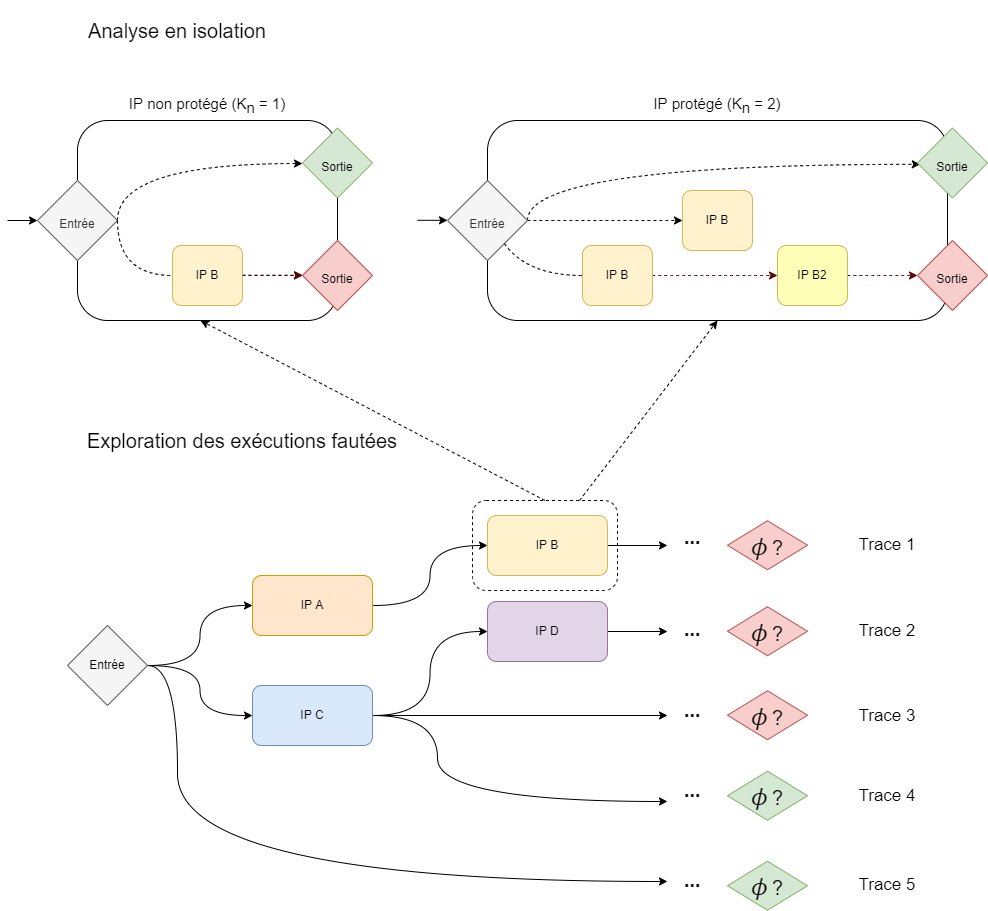
\includegraphics[scale=0.39]{ch5-placement/img/placement-isolation.drawio.png}
                    \caption{Principe général du placement avec analyse en isolation}
                    \label{fig:placement-isol}
                \end{figure}
            
                L'exploration des traces d'attaque donne des informations sur les relations entre les entrées et les sorties des différents points d'injection.   
                L'objectif est de déterminer si un \gls{ip} peut être protégé partiellement (avec un coefficient de protection inférieur à $n + 1$), sans que la sortie invalide qu'il produira n'introduise de nouveaux chemins fautés qui n'auraient pas été pris en compte.            
                Dans la figure \ref{fig:placement-isol}, l'exploration des chemins fautés (en bas), contient des informations sur les effets possibles d'une sortie corrompue d'un point d'injection. Les losanges verts indiquent que l'objectif d'attaque n'est pas validé (attaque non réussie), et les losanges rouges indiquent une attaque réussie.
                
                Par exemple, si on s'intéresse à la trace $2$, comportant la séquence de points d'injection déclenchés $\{ IP_C, IP_D \}$, on peut déterminer qu'un coefficient de protection de $3$ pour $IP_C$ serait suffisant pour obtenir une robustesse en 3 fautes\footnote{Pour $K_n = 3$, la Trace $4$ deviendrait une attaque en $4$ fautes, une faute étant nécessaire pour casser le point d'injection $IP_D$ non protégé.}.
                On peut alors se poser la question de si une attaque en 3 fautes est possible après la sortie invalide de l'\gls{ip} $IP_C$, qui ne demande que 3 fautes pour être corrompue.
                La réponse est donnée par l'exploration complète des traces d'attaques. La trace $4$ est une attaque non réussie et n'est donc pas à prendre en compte.
                En revanche la trace $3$ indique que si $IP_C$ n'est protégé qu'avec un coefficient de protection de $3$, alors la sortie invalide de $IP_C$ peut produire une attaque en $3$ fautes. Un coefficient de protection d'au moins $4$ est nécessaire sur $IP_C$ pour garantir la robustesse en 3 fautes.
    
                L'objectif est de pouvoir substituer les comportements des \gls{ip}s protégés à ceux des \gls{ip}s non protégés qui sont analysés dans l'exploration des exécutions fautées sur $P$, de manière à pouvoir prévoir comment un \gls{ip} protégé va se comporter dans le contexte du programme. 
                L'analyse en isolation abstrait les comportements fautés dans l'\gls{ip}, mais il est nécessaire de garantir que les comportements produits par un point d'injection fauté sont bien inclus dans les modèles de faute utilisés dans l'exploration préliminaire des exécutions fautées. 
                Dans le cadre des modèles de faute \gls{TI} et \gls{DL}, les sorties invalides d'un \gls{ip} fautés sont en effet incluses dans les modèles de Lazart:
                \begin{itemize}
                    \item Pour \gls{TI}, les différents schémas de protection de \gls{TM} peuvent produire une sortie vers la mauvaise branche.
                    \item Pour \gls{DL}, les différents schémas de protection de \gls{LM} peuvent produire une valeur erronée lue par le \texttt{load}, qui correspond au modèle \gls{DL}.
                \end{itemize}
    
                Ce ne serait pas le cas avec tous les modèles. Par exemple une mutation de donnée en mise-à-zéro, pourrait potentiellement produire des comportements différents (comme une mise-à-un) en fonction du schéma de protection.
                Pour garantir la possibilité de substituer les \gls{ip} protégés et non protégés, il serait nécessaire de montrer que les schémas de protection ne peuvent produire que le comportement nominal ou des mises-à-zéro, ou bien utiliser un modèle de mutation de donnée général (symbolique) dans l'exploration des chemins fautés afin de garantir cette inclusion.
     
            \subsubsection{Un problème d'optimisation linéaire}
            \label{sec:placement-optimal-ilp}
    
                La recherche des meilleurs placements répartis (dont le total des pondérations de protection appliquées et minimal) correspond à la recherche des ensembles de coefficients de protection minimaux tels que toute attaque réussie dans $T(P', M)$ nécessite au moins $n + 1$ fautes. 
                L'idée est de couvrir toutes les attaques, chaque attaque donnant un ensemble de contraintes sur les coefficients de protection à appliquer à chaque \gls{ip} pour obtenir la garantie de robustesse. On peut notamment remarquer:
                \begin{itemize}
                    \item si plusieurs \gls{ip}s apparaissent dans une attaque, alors chaque \gls{ip} peut être protégé indépendamment pour obtenir au final une attaque en plus de $n$ fautes.
                    \item si un point d'injection $ip$ apparaît $x$ fois dans une attaque, alors une protection sur $ip$ ajoute la nécessité de $x*K_n$ fautes supplémentaires.
                \end{itemize}        
        
                Les contraintes imposées par une attaque $a$ peuvent se traduire par une inégalité $C_a$ de la forme $\alpha x_1 + ... + \gamma x_n \geq n + 1$, avec $n$ le nombre de fautes pour lequel $P$ doit être robuste, $\{x_1, ..., x_n\}$ les coefficients de protection des \gls{ip}s $\{1, ..., n\}$ et $\{\alpha, ..., \gamma\}$ les coefficients correspondants au nombre de fois où chaque point d'injection se déclenche dans l'attaque.
                La figure \ref{fig:placement-ineq} présente des exemples de traces d'attaques à partir desquelles les inégalités sont générées (indiquées à droite), où \textit{faute X} désigne le déclenchement d'une faute sur le point d'injection $X$.  
                
                \begin{figure}[!h]\centering
                    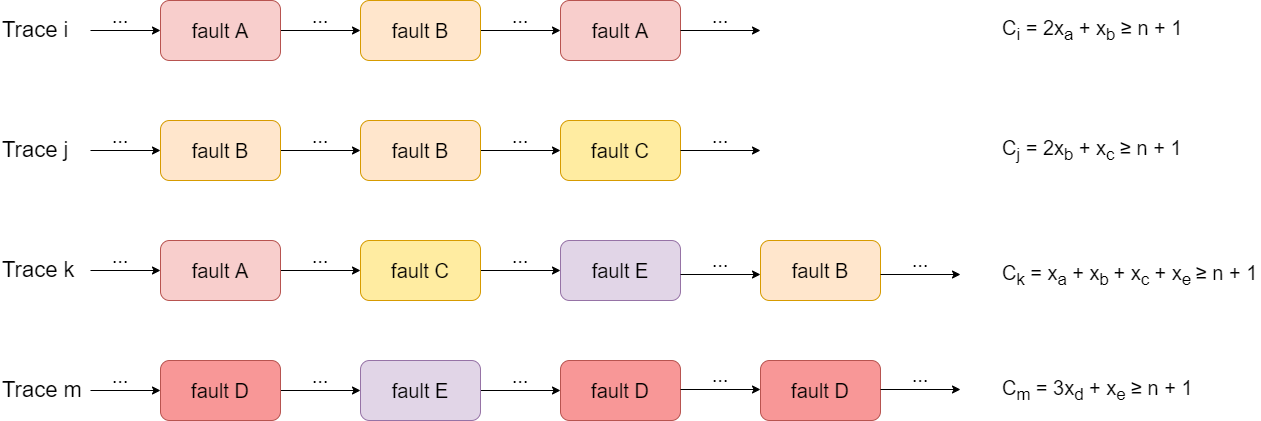
\includegraphics[scale=0.29]{ch5-placement/img/placement-eq.drawio.png}
                    \caption{Inégalités sur les coefficients de protection à partir des attaques}
                    \label{fig:placement-ineq}
                \end{figure}
                
                L'objectif est de trouver les ensembles de coefficients ($\{x_1, ..., x_n\}$) validant les contraintes $C_i$ et minimisant la fonction $x_1 + x_2 + ... + x_n$. 
                Ce problème est une instance du problème d'optimisation linéaire en nombre entier, \gls{ilp}, qui est NP-complet.
        
            \subsubsection{Algorithme de placement réparti optimal}
            \label{sec:placement-optimal-algo}
            
                Le listing \ref{lst:optimal-placement} présente l'algorithme de placement réparti optimal (\textit{rep-opt}) qui s'appuie aussi sur les attaques minimales.
                Dans un premier temps, les contraintes du problème d'optimisation linéaire sont générées à partir des attaques (fonction \texttt{compute\_constraint} ligne 12) et le problème d'optimisation linéaire est résolu dans la fonction \texttt{solve\_ilp} (ligne 14), qui fournit ainsi l'ensemble des coefficients minimisant la somme des protections appliquées.
                Le programme $P'$ est ensuite généré en appliquant les contre-mesures avec les coefficients de protection obtenus.

\lstset{caption={Algorithme de placement réparti optimal \texttt{rep-opt}},label=lst:optimal-placement}
\begin{lstlisting}  
def placement_rep_opt(C: Catalog, P: Program, M: AttackModel, n: int):
    # Get sucessfull non-detected attacks.
    attacks = T_s(P, M, n)
    # Filter with minimals attacks.
    minimals = RedundacyAnalysis(attacks).minimals()
    
    # Initial protection factors Kn at 1 for all IP.
    required_kn = { IPA: 1, IPB: 1, ..., IPN: 1 }
    
    constraints = [] # constraints for ILP
    for attack in minimals:
        constraints += compute_constraint(attack)
    
    required_kn = solve_ilp(constraints, required_kn)
    
    # Generation of P'
    P` = P
    for IP, kn in required_kn:
        S = C.get_cm(IP.model(), kn) # Select protection scheme from catalog
        P` = S(P`, IP) # Apply local protection        
    return P`
\end{lstlisting} 

                Dans le cadre d'un catalogue adapté et complet pour le modèle $m$, $P'$ est robuste en au moins $n$ fautes et la somme des coefficients de protection appliqués est minimale.
    
        \subsection{Autres algorithmes de placement}
        \label{sec:placement-other}

            Trois approches de placement ont été abordées précédemment: le placement systématique (algorithmes \textit{naïf}, \textit{atk} et \textit{min}), le placement par bloc par heuristiques (\textit{bloc-h}) et le placement réparti optimal (\textit{rep-opt}).
            Cette section discute de certaines variantes possibles de ces algorithmes.
            
            \paragraph{Catalogue non total}
            Les sections précédentes ont considéré des catalogues qui possèdent toujours un schéma de protection avec le coefficient de protection demandé.
            On considérera ici un catalogue non total, qui dispose d'une fonction \textit{catalog.get\_cm(IP, k)}, retournant le couple $(S, k')$, avec $S$ le schéma de protection et $k'$ le coefficient de protection de $S$. Deux cas peuvent être distingués : 
            \begin{itemize}
                \item \textit{Sur-protection} : le catalogue fournit le schéma de protection avec $k'$ le plus petit, tel que $k' > k$.
                \item \textit{Sous-protection} : le catalogue fournit un schéma avec $k' < k$.
            \end{itemize}
    
            La \textit{sur-protection} préserve la robustesse du programme protégé. Dans le cas de l'algorithme optimal néanmoins, il devient nécessaire d'ajouter une contrainte supplémentaire sur les coefficients de protection requis pour certains \gls{ip}s. Cela peut donc faire sortir le problème du cadre de l'\gls{ilp} (ce qui ne le rend pas pour autant indécidable), en ajoutant des contraintes du type $X_a \neq 2$ (pour représenter l'absence de schéma pour $K_n = 2$).
            Dans le cas d'une \textit{sous-protection}, le problème de sortie du cadre du problème \gls{ilp} se pose aussi.
            Plus encore, la robustesse du programme peut être remise en question. Si un autre \gls{ip} peut être protégé avec un coefficient de protection suffisant, alors il est possible de garantir la robustesse du programme (quelle que soit l'approche de placement utilisée).
            S'il existe des traces d'attaques pour lesquelles il n'est pas possible de protéger pour $n$ fautes en raison d'un manque de schéma de protection adapté, alors la robustesse en $n$ fautes du programme $P'$ est perdue.
            Ces traces d'attaques sont cependant connues au moment du placement et peuvent être retournées à l'utilisateur, permettant d'anticiper les traces d'attaques du programme $P'$ sans avoir à en explorer les chemins fautés et de déterminer le nombre de fautes pour lequel $P'$ est robuste (en calculant la somme des coefficients de protection des \gls{ip} de chaque attaque non protégée).
             
            \paragraph{Placement réparti par heuristique}
            On peut construire l'algorithme \textit{rep-h} correspondant au placement réparti utilisant des heuristiques plutôt qu'un problème \gls{ilp}.
            Cet algorithme fonctionne comme \textit{bloc-h} (listing \ref{lst:placement-bloc-h}), en combinant une heuristique de parcours des traces et une heuristique de sélection des \gls{ip}s à protéger dans une trace.
            Cette approche peut être préférée à l'approche \textit{rep-opt} (listing \ref{lst:optimal-placement}) dans le cas où :
            \begin{itemize}
                \item le problème \gls{ilp} de l'approche optimale est trop complexe pour être résolu.
                \item certaines contraintes sur le catalogue sortent du cadre du problème \gls{ilp} standard.
            \end{itemize}
             
            \paragraph{Placement optimal par bloc}         
            L'algorithme \textit{bloc-h} ne garantit pas l'optimalité du placement par bloc. Un algorithme de placement optimal par bloc (visant à protéger le moins d'\gls{ip}s possible avec un $K_n = n+1$) est envisageable.
            Le placement \textit{bloc-h} nécessite cependant des contraintes qui ne sont pas de l'ordre du problème \gls{ilp} (les coefficients n'étant plus bornés entre $1$ et $n + 1$ mais ne pouvant prendre que l'une des deux valeurs).
            Cet algorithme correspond à rechercher l'ensemble minimum d'\gls{ip} qui couvrent toutes les traces d'attaques minimales au moins une fois, ce qui se rapproche de l'algorithme de sélection présenté dans le chapitre suivant (voir section \ref{sec:ch6-impl-selection}). 
            
    \section{Expérimentation}
    \label{sec:placement-exps}
        
        Cette section présente quelques expérimentations qui ont été menées sur les algorithmes de placement présentés précédemment : 
        \begin{itemize}
            \item \textit{naïf} (section \ref{sec:placement-syst}) : protection avec $K_n = n+1$ de tous les \gls{ip}s du programme.
            \item \textit{atk} (section \ref{sec:placement-syst}) : protection avec $K_n = n+1$ de tous les \gls{ip}s intervenant dans les attaques.
            \item \textit{min} (section \ref{sec:placement-syst}) : protection avec $K_n = n+1$ de tous les \gls{ip}s intervenant dans les attaques minimales.
            \item \textit{bloc-h} (section \ref{sec:placement-bloc}) : protection avec $K_n = n+1$ d'au moins un \gls{ip} par attaque minimale avec heuristiques.
            \item \textit{rep-opt} (section \ref{sec:placement-opti}) : algorithme optimal pour la protection répartie entre les \gls{ip}s.
        \end{itemize}
            
        \begin{figure}[!h]\centering
            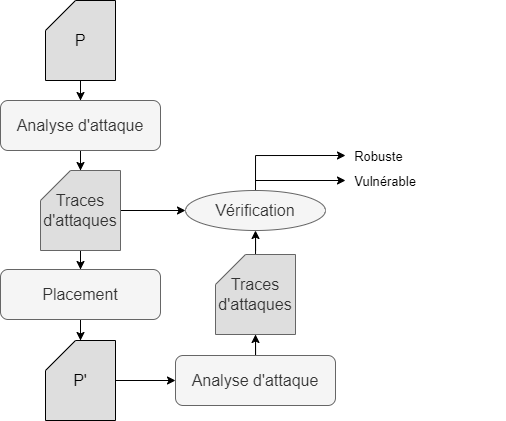
\includegraphics[scale=0.45]{ch5-placement/img/placement-exps.drawio.png}
            \caption{Méthodologie expérimentale pour les algorithmes de placement}
            \label{fig:placement-exp-clpp}
        \end{figure}
        
        La figure \ref{fig:placement-exp-clpp} présente la méthodologie expérimentale utilisée. Chaque algorithme prend en entrée les traces d'attaques générées par Lazart, et retourne les protections à appliquer pour générer le programme $P'$. 
        Une analyse d'attaque est effectuée sur $P'$, permettant ainsi de déterminer si le programme est robuste en $n$ fautes (ce qui n'est garantit que si l'exécution symbolique est complète et correcte).
        Pour l'algorithme de placement optimal (\textit{rep-opt}), la résolution du problème d'optimisation linéaire a été réalisée avec un outil en ligne \footnote{L'annexe \ref{annexe:ilp-memcmp} présente les fichiers de contraintes fournis à l'outil en ligne (\url{https://online-optimizer.appspot.com}).}.
        
        La section \ref{sec:placement-exp-cms} décrit les catalogues de contre-mesures utilisés en fonction du modèle de faute considéré.
        La section \ref{sec:placement-exp-prgm} présente les programmes étudiés et les objectifs d'attaques et la section \ref{sec:placement-exp-res} discute des résultats obtenus.

        \subsection{Catalogue de contre-mesures et inversion de branches}
        \label{sec:placement-exp-cms}

            La section \ref{sec:ch6-defs} a présenté la contre-mesure de multiplication de tests qui est adaptée pour le modèle de l'inversion de test.
            Ses schémas de protection protègent à la fois la branche \textit{vrai} et la branche \textit{faux} de chaque test.

            Dans ces expérimentations, on s'intéressera à une variation de cette contre-mesure qui vise à protéger une seule branche d'un test, permettant ainsi de protéger chaque branche avec une pondération différente.
            Cela nécessite de considérer un autre modèle que l'inversion de test, qu'on appellera \textit{inversion de branche} (\gls{BI}), et pour lequel les points d'injection de la branche \textit{vrai} et la branche \textit{faux} sont distincts.

            Lazart ne supporte pas directement le modèle de l'inversion de branche, mais il est possible d'appliquer une analyse en inversion de test et de distinguer à posteriori les fautes concernant la branche \textit{vrai} et la branche \textit{faux}.

            Les expérimentations utilisent un catalogue de contre-mesures complet et adapté pour le modèle de faute considéré. Ce catalogue retourne le schéma de protection à appliquer pour un point d'injection et un coefficient de protection donnés. 
            Dans le cadre de \gls{BI}, on utilisera donc la multiplication de test sur la branche correspondant au point d'injection.
            Pour le modèle \gls{DL}, on utilisera la multiplication de load.
            Le catalogue garantit ainsi qu'un schéma de protection de profondeur $n$ offre un coefficient de protection de $n + 1$.
        
        \subsection{Programmes utilisés}
        \label{sec:placement-exp-prgm}

            Les programmes étudiés dans cette section sont les suivants:
            \begin{itemize}
                \item \textit{verify pin 2b} (\texttt{vp2b}).
                \item \textit{firmware updater 1} (\texttt{fu1}).
                \item \textit{memcmps} (\texttt{memcmps3}).
            \end{itemize}
    
            \texttt{vp2b} correspond à une version modifiée de \textit{verify\_pin} 2 (voir annexe \ref{annexe:prgm:vp2b}), qui comprend les booléens endurcis et la boucle en temps constant mais ne possède pas de contre-mesure vérifiant le compteur de boucle (l'idée étant de placer les schémas de protection). \texttt{vp2b} est analysé uniquement avec le modèle \gls{BI} et avec l'objectif d'attaque visant à s'authentifier avec un \gls{pin} faux. Les tableaux d'entrées sont symboliques, de taille 4 et différents sur au moins un octet.
    
            \texttt{fu1} (voir section \ref{sec:lz:exp:bench}) à l'inverse contient une duplication de test systématique et considère les modèles \gls{BI} et \gls{DL}. L'objectif d'attaque vise soit à charger un micro-programme corrompu, soit à ne pas mettre à jour le micro-programme.
    
            \texttt{memcmps3} correspond à une version durcie du programme présenté dans la section \ref{sec:lz:memcmps} (voir annexe \ref{annexe:prgm:memcmps3}), dans laquelle quatre appels successifs à \texttt{memcmp} sont effectués avec différents masques. Les tableaux d'entrées sont symboliques et différents (sur au moins un octet) et l'objectif est de retourner $vrai$ malgré l'inégalité des tableaux.
            Le programme est analysé avec les modèles \gls{BI} et \gls{DL}. 
        
        \subsection{Comparaison des algorithmes de placement}
        \label{sec:placement-exp-res}

            La table \ref{tbl:placement-exp-clpp} présente les résultats obtenus pour les différents programmes.
            La colonne "Expé" indique les paramètres de l'expérimentation avec "P" le programme utilisé, "m" le modèle de faute considéré et "IPs" le nombre total de points d'injection dans le programme.
            La colonne "Algos" indique quel algorithme de placement est utilisé.
            La colonne "$\sum$ de protections" indique la somme des pondérations de protection\footnote{Correspondant au coefficient de protection appliqué pour chaque \gls{ip} moins 1 (un \gls{ip} non protégé ayant un coefficient de protection de 1).} appliquées par le placement.
            Enfin la colonne "Robuste" indique si le programme protégé $P'$ est robuste en $n$ fautes après une analyse de vérification avec Lazart.
            
            \begin{table}[htp]
                {\small
                \begin{center}
                    \begin{tabular}{lll|l|llll|l}
                    \multicolumn{3}{c}{Expé} & \multicolumn{1}{c}{Algo.} & \multicolumn{4}{c}{$\sum$ des protections} & \multicolumn{1}{c}{Robuste} \\
                    \hline
                    P & m & IPs &  & 1 faute & 2 fautes & 3 fautes & 4 fautes &  \\
                    \hline
                    \hline
                    \texttt{vp2b} & BI & \multicolumn{1}{r|}{8} & naïf & 8 & 16 & 24 & 32 & \checkmark \\
                     &  &  & atk & \textbf{3} & 8 & 12 & 16 & \checkmark \\
                     &  &  & min & \textbf{3} & 8 & 12 & 16 & \checkmark \\
                     &  &  & bloc-h & \textbf{3} & \textbf{6} & \textbf{9} & \textbf{12} & \checkmark \\
                     &  &  & rep-opt & \textbf{3} & \textbf{6} & \textbf{9} & \textbf{12} & \checkmark \\
                    \hline
                    \hline
                    \texttt{fu1} & BI & \multicolumn{1}{r|}{42} & naïf & 42 & 84 & 126 & 168 & \checkmark \\
                     &  &  & atk & \textbf{0} & 28 & 42 & 88 & \checkmark \\
                     &  &  & min & \textbf{0} & 28 & 42 & 72 & \checkmark \\
                     &  &  & bloc-h & \textbf{0} & 14 & 21 & 28 & \checkmark \\
                     &  &  & rep-opt & \textbf{0} & \textbf{7} & \textbf{14} & \textbf{21} & \checkmark \\
                    \hline
                     & DL & \multicolumn{1}{r|}{2} & naïf & 2 & 4 & 6 & 8 & \checkmark \\
                     &  &  & atk & \textbf{1} & 4 & 6 & 8 & \checkmark \\
                     &  &  & min & \textbf{1} & \textbf{2} & \textbf{3} & \textbf{4} & \checkmark \\
                     &  &  & bloc-h & \textbf{1} & \textbf{2} & \textbf{3} & \textbf{4} & \checkmark \\
                     &  &  & rep-opt & \textbf{1} & \textbf{2} & \textbf{3} & \textbf{4} & \checkmark \\
                    \hline
                     & BI+DL & \multicolumn{1}{r|}{44} & naïf & 44 & 88 & 132 & 176 & \checkmark \\
                     &  &  & atk & \textbf{1} & 32 & 60 & 96 & \checkmark \\
                     &  &  & min & \textbf{1} & 32 & 60 & 80 & \checkmark \\
                     &  &  & bloc-h & \textbf{1} & 16 & 24 & 32 & \checkmark \\
                     &  &  & rep-opt & \textbf{1} & \textbf{9} & \textbf{17} & \textbf{25} & \checkmark \\
                    \hline
                    \hline
                    \texttt{memcmps3} & BI & \multicolumn{1}{r|}{12} & naïf & 12 & 24 & 36 & 48 & \checkmark \\
                     &  &  & atk & \textbf{0} & \textbf{0} & \textbf{0} & 16 & \checkmark \\
                     &  &  & min & \textbf{0} & \textbf{0} & \textbf{0} & 16 & \checkmark \\
                     &  &  & bloc-h & \textbf{0} & \textbf{0} & \textbf{0} & 4 & \checkmark \\
                     &  &  & rep-opt & \textbf{0} & \textbf{0} & \textbf{0} & \textbf{1} & \checkmark \\
                    \hline
                     & DL & \multicolumn{1}{r|}{15} & naïf & 15 & 30 & 45 & 60 & \checkmark \\
                     &  &  & atk & \textbf{1} & 6 & 15 & 32 & \checkmark \\
                     &  &  & min & \textbf{1} & 6 & 15 & 32 & \checkmark \\
                     &  &  & bloc-h & \textbf{1} & 4 & 6 & 8 & \checkmark \\
                     &  &  & rep-opt & \textbf{1} & \textbf{3} & \textbf{4} & \textbf{7} & \checkmark \\
                    \hline
                     & BI+DL & \multicolumn{1}{r|}{27} & naïf & 27 & 54 & 81 & 108 & \checkmark \\
                     &  &  & atk & \textbf{1} & 8 & 24 & 56 & \checkmark \\
                     &  &  & min & \textbf{1} & 8 & 24 & 56 & \checkmark \\
                     &  &  & bloc-h & \textbf{1} & 6 & 9 & 12 & \checkmark \\
                     &  &  & rep-opt & \textbf{1} & \textbf{3} & \textbf{4} & \textbf{9} & \checkmark
                    \end{tabular}
                \end{center}
                }
                \label{tbl:placement-exp-clpp}
                \caption{Comparaison des différents algorithmes de placement}
            \end{table}

            Comme attendu, l'approche par bloc (\textit{bloc-h}) offre de meilleurs résultats que les approches systématiques. De la même manière, le placement réparti (\textit{rep-opt}) produit un poids de protection plus faible.
            
            Pour l'exemple \texttt{vp2b}, on constate que les algorithmes \textit{min} et \textit{atk} sont équivalents, tous les \gls{ip}s des attaques intervenant aussi dans les attaques minimales.
            Les algorithmes \textit{bloc-h} et \textit{rep-opt} fournissent les mêmes résultats, ce qui s'explique par un grand nombre d'attaques en 1 faute qui imposent une pondération de $n \in \mathbb{N}^*$ aux points d'injection concernés pour être résistant en $n$ fautes.

            Pour \texttt{fu1}, seuls deux points d'injection sur les données sont présents et l'un d'entre eux intervient dans une attaque en une faute. Ce même point d'injection est donc à protéger avec un coefficient de protection $K_n = n + 1$ dans le cas du modèle $BI + DL$.
            On observe pour le modèle $BI + DL$ que les algorithmes proposent tous des résultats différents, mettant en évidence la relation d'ordre entre les résultats de chaque algorithme. 

            Pour l'exemple \texttt{memcmps3}, on peut constater un net avantage des algorithmes prenant en compte les attaques pour le modèle \gls{BI}. En effet, une seule attaque est possible avec ce modèle, et consiste à inverser chacun des quatre appels à \texttt{memcmp}. 
            L'algorithme optimal ne nécessite qu'un coefficient de protection $K_n = 2$ puisque déjà quatre fautes sont nécessaires pour l'attaque. 
            Dans cet exemple, les résultats pour l'algorithme \textit{rep-opt} sont meilleurs que \textit{bloc-h} quel que soit le modèle de faute.
            
            On peut remarquer que le programme $P'$ est robuste pour toutes les expérimentations réalisées. Cela peut faire penser que l'exploration des chemins est complète pour tous les programmes.
            Cependant, on peut postuler que si l'exploration rate des chemins pour la génération des attaques sur $P$, il est probable que les chemins correspondant dans $P'$ sont eux aussi manqués.

    \section{Protégeabilité et contre-mesure parfaite}
    \label{sec:model-protectability}

        Les différents algorithmes de placement présentés dans ce chapitre posent des conditions fortes sur les propriétés des contre-mesures du catalogue (adéquation et coefficient de protection suffisant) lorsqu'on recherche une robustesse en $n$ fautes.
        Cette section propose une classification des modèles de faute en fonction du type de protection qu'il est possible d'y appliquer.
        
        On notera $\mathcal{M}$ l'ensemble des modèles de faute.
        Il existe des modèles pour lesquels il est possible de protéger un programme pour le rendre résistant en $n$ fautes, on dit alors que le modèle de faute est \textit{protégeable} (comme les modèles \gls{TI} et \gls{DL}).
        A l'inverse, il existe des modèles pour lesquels il n'est pas possible de se protéger en $n$ fautes. Given et al \cite{Given/ICESS17} ont montré l'existence de tels modèles en se ramenant à des machines de Turing.
        C'est le cas par exemple d'un modèle de remplacement d'instruction arbitraire, permettant de remplacer le programme en un autre de taille arbitraire.
        On divisera donc l'ensemble des modèles de faute en fonction de leur \textit{protégeabilité}:
        
        \begin{itemize}
            \item $\mathcal{P}$ (\textit{modèles Protégeables}): $m \in \mathcal{P} \iff  \exists C $ tel que $\forall \; programme \; P, \forall n \in \mathbb{N}$, $T_s(C(P), m_n) = \emptyset$\footnote{Avec $T_s(P, m_n)$ correspondant à l'ensemble des attaques réussies pour $P$ jusqu'à $n$ fautes.}.
            \item $\mathcal{N}$ (\textit{modèles Non protégeables}): $m \in \mathcal{P} \iff  \nexists C $ tel que $\forall \; programme \; P, \forall n \in \mathbb{N}$, $T_s(C(P), m_n) = \emptyset$ 
        \end{itemize}
        
        L'ensemble des modèles protégeables $\mathcal{P}$ peut être divisé en deux sous-ensembles.
        Les modèles pour lesquels il existe une Contre-mesure Locale Pondérée et Adaptée (CLP-A) sont dits \textit{localement protégeables}, notés  $\mathcal{L}$ et ceux pour lesquels il n'en existe pas sont appelés \textit{globalement protégeables}, notés $\mathcal{G}$. 
        Les modèles pour lesquels il existe une contre-mesure locale parfaite sont dits \textit{parfaitement protégeables}, notés $\mathcal{F}$.
        
        Dans le cas des modèles non protégeables ($\mathcal{N})$, on peut là encore diviser entre ceux pour lesquels il est possible de rendre les attaques plus difficiles à réaliser, qu'on appellera \textit{modèles diluables} $\mathcal{D}$ et ceux pour lesquels cela n'est pas possible, appelés \textit{modèles strictement non protégeables}, notés $\mathcal{S}$.
        
        \begin{figure}[!h]\centering
            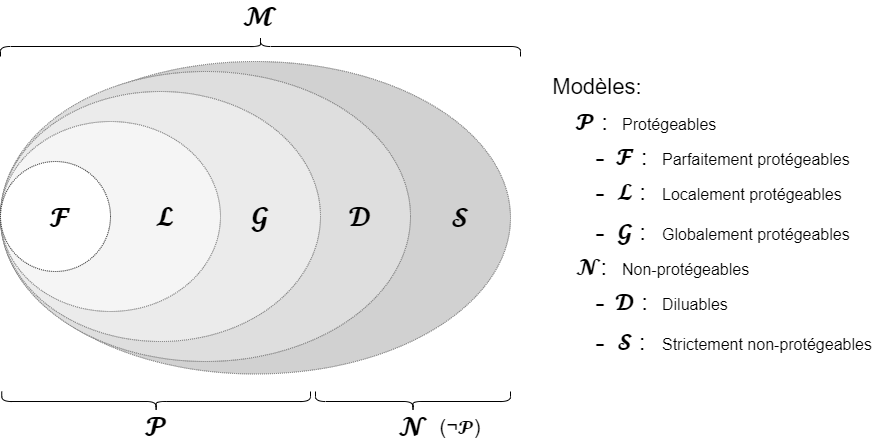
\includegraphics[scale=0.4]{ch5-placement/img/protectable-models-set-extended.drawio.png}
            \caption{Classification des modèles d'attaquant en fonction de leur \textit{protegeabilité}}
            \label{fig:models-protectability}
        \end{figure}
        
        La figure \ref{fig:models-protectability} présente une classification des modèles d'attaquant en fonction de leur protégeabilité. 
        Plusieurs questions restent en suspens concernant l'existence de certaines sous-classes.
        Les sections précédentes ont présenté des modèles dans $\mathcal{L}$ (\textit{localement protégeables}), avec les exemples des modèles \gls{TI}, \gls{DL} et $TI+DL$, pour lesquelles les contre-mesures locales \gls{TM}, \gls{LM} et \gls{TLM} ont été proposées.
        Les modèles \textit{globalement protégeables} ($\mathcal{G}$) sont des modèles pour lesquels il existe une transformation du programme (non locale) permettant de rendre le programme robuste en $n$ fautes. L'existence de cette classe de modèles est hypothétique puisque nous n'avons pas trouvé d'exemple, mais ne semble pas impossible pour autant.
        Il semble difficile de construire une contre-mesure parfaite pour les modèles \gls{TI} et \gls{DL} par exemple, mais l'existence de modèles dans $\mathcal{F}$ semble tout de même probable, si l'on s'intéresse à des modèles de faute simples.
        Formulé autrement: $\mathcal{L} = \mathcal{G} = \mathcal{P} ?$ (considérant que $\mathcal{G}$ n'inclut pas $\mathcal{L})$.
        
        Une autre question survient avec cette classification: est-ce qu'un modèle peut changer de classe de \textit{protégeabilité} si on s'intéresse qu'à un sous-ensemble des programmes possibles à protéger et/ou à un sous-ensemble des objectifs d'attaque.
        Il est aussi possible que cette classification n'ait de sens que si on exclut effectivement certains programmes et objectifs d'attaque qui sont toujours \textit{protégeables} ou \textit{non protégeables} quel que soit le modèle de faute \footnote{Par exemple si un modèle $m$ est non protégeable dans le cas général, mais protégeable si on exclut le programme vide, peut-être faudrait-il le considérer comme protégeable et simplement exclure ce cas extrême de la définition.}.
        Cette question n'a pas été explorée davantage.    
        On peut aussi noter que ce n'est pas parce qu'un modèle de faute est non protégeable qu'il n'existe pas de protection contre ce type d'attaques en considérant un autre niveau de représentation.
        
        Enfin, il est raisonnable de se demander à quel point les modèles \textit{localement protégeables} ($\mathcal{L})$ sont suffisamment réalistes pour être utilisés pour le placement de contre-mesures en pratique.
        On peut arguer à cette question que, même s'il s'avère que les modèles dans $\mathcal{L}$ sont en réalité trop rares ou trop spécifiques, il reste envisageable que cette méthodologie puisse être généralisée pour le calcul du placement de contre-mesures pour des modèles dans $\mathcal{G}$.
        
        Cette classification des modèles en fonction de leur protégeabilité contient donc encore des classes qui sont hypothétiques et des travaux futurs pourraient viser à préciser cela.
    
    \section{Conclusion et perspectives}
    \label{sec:placement-fw}
    
        Cette section présente une conclusion de ce chapitre et discute des perspectives possibles de ces travaux.
        
        \subsection{Conclusion}
        
            La table \ref{tbl:placement-conclusion} présente une comparaison des algorithmes de placement présentés dans ce chapitre (identifiés en colonne "Algo"):
            \begin{itemize}
                \item \textit{naïf}: protection systématique de tous les \gls{ip}s avec $K_n = n + 1$.
                \item \textit{atk}: protection des \gls{ip}s des attaques avec $K_n = n + 1$.
                \item \textit{min}: protection des \gls{ip} des attaques minimales avec $K_n = n + 1$.
                \item \textit{bloc-h}: algorithme par bloc avec heuristiques.
                \item \textit{rep-opt}: algorithme optimal réparti.
                \item \textit{bloc-opt}: algorithme par bloc optimal.
                \item \textit{rep-h}: algorithme réparti avec heuristiques.
            \end{itemize}
            La colonne "Type" indique le type de placement de l'algorithme: \textit{systématique}, par \textit{bloc} ou \textit{réparti}.
            Les colonnes "Garanties $P'$" indiquent les garanties pour le programme $P'$ en ce qui concerne la robustesse du programme $P'$ pour un catalogue total. L'optimalité du placement indique si le placement est optimal par rapport au type de placement considéré.            
            La colonne "Complexité" indique la complexité de l'algorithme de placement (donc sans prendre en compte les différentes analyses d'attaques, de points chauds ou de redondance éventuelles), $t$ correspondant au nombre d'attaques minimales obtenues par l'analyse d'attaque.
            Les colonnes "Analyses" indiquent les analyses de Lazart utilisées pour l'algorithme: analyse d'attaques ($AA$), analyse de redondance ($Red$) et analyse de points chauds ($HS$).

            \begin{table}[h]
                {\small
                \begin{center}
                    \begin{tabular}{l|l|ll|l|lll}
                    Algorithme & Type & \multicolumn{2}{l|}{Garanties $P'$} & Complexité & \multicolumn{3}{l}{Analyses requises} \\
                     &  & Robuste & Optimal &  & AA & Red & HS \\
                     \hline
                    naïf & syst. & \checkmark & - & $O(t)$ & \checkmark & - & - \\
                    atk & syst. & \checkmark & - & $O(t)$ & \checkmark & - & - \\
                    min & syst. & \checkmark & - & $O(t)$ & \checkmark & \checkmark & - \\
                    bloc-h & bloc & \checkmark & - & $O(t)$ & \checkmark & \checkmark & \checkmark \\
                    rep-opt & réparti & \checkmark & \checkmark & NP-Complet$^1$ & \checkmark & \checkmark & - \\
                    bloc-opt & bloc & \checkmark & \checkmark & NP-Complet$^1$ & \checkmark & \checkmark & - \\
                    rep-h & réparti & \checkmark & - & $O(t)$ & \checkmark & \checkmark & \checkmark
                    \end{tabular}
                \end{center} 
                }
                
                \caption{Comparaison des différentes approches de placement}
                \label{tbl:placement-conclusion}
            \end{table}
            
            \footnotetext[1]{L'\gls{ilp} est NP-Complet dans le cas général mais les contraintes générées dans le cas des placements optimaux restent relativement simples.}
  
            Les expérimentations ont montré que les différents algorithmes parviennent à rendre un programme robuste en $n$ fautes lorsque le catalogue est total. 
            On peut constater la relation d'ordre attendue entre les poids de protections proposés par les différents algorithmes de placement : \textit{naïf} $\geq$ \textit{atk} $\geq$ \textit{min} $\geq$ \textit{bloc-h} $\geq$ \textit{bloc-opt} $\geq$ \textit{rep-h} $\geq$ \textit{rep-opt}. 
            Les algorithmes de placement systématiques produisent un grand nombre de protections superflues par rapport aux autres approches, mais les résultats dépendent grandement du programme considéré, \textit{min} trouvant le placement optimal dans l'exemple \texttt{fu1} avec \gls{DL} par exemple.
            De la même manière, \textit{bloc-h} peut parfois donner les mêmes résultats que \textit{rep-opt}, comme pour \texttt{vp2b}.
            
            La complexité du placement optimal (section \ref{sec:placement-opti}) rend son passage à l'échelle difficile pour des programmes contenant des combinaisons de placements possibles élevées. Néanmoins, les expérimentations tendent à montrer que l'ensemble des contraintes générées pour le problème d'optimisation linéaire est souvent simple, même dans le cas de programmes complexes. Cela est du aux attaques en une faute imposant un coefficient de protection maximal (c'est-à-dire de $n + 1$) à certains points d'injection.
            
            L'analyse en isolation (section \ref{sec:ooc}) des schémas de protection permet d'obtenir des garanties en fautes multiples concernant l'efficacité d'une contre-mesure sur un point d'injection, en fonction d'un modèle de faute. En combinaison avec l'exploration des chemins fautés, il est possible d'anticiper les comportements des programmes protégés en fonction des coefficients de protection appliqués.
            Dans le cas de catalogue non totaux, il est possible de prévoir si un placement va produire un programme $P'$ robuste si un cas de sous-protection est rencontré (section \ref{sec:placement-other}), et dans ce cas de fournir les attaques de $P'$.
            Si l'exploration des chemins d'attaque n'est pas complète, on a tout de même la garantie d'avoir protégé certaines attaques sans en avoir introduit de nouvelles, ce qui permet à $P'$ d'être \textit{au moins aussi robuste} que $P$, sans garantie de robustesse en $n$ fautes.
    
        \subsection{Perspectives}
        
            Différentes perspectives peuvent être envisagées pour les travaux présentés dans ce chapitre. Dans un premier temps, il serait intéressant d'étendre les exemples de programmes et de contre-mesures pour comparer plus en profondeur les diverses approches.
            Les algorithmes \textit{bloc-opt} et \textit{rep-h} pourraient être implémentés afin de pouvoir les comparer expérimentalement avec les autres algorithmes, mais ils n'offriront pas de meilleures garanties que \textit{rep-opt}.            
            Pour terminer sur le plan implémentation, l'algorithme de placement optimal utilise pour le moment une intervention manuelle de l'utilisateur pour l'appel à un outil d'optimisation linéaire et automatiser ce processus serait un plus.
            
            De la même manière, d'autres modèles de faute pourraient être considérés, notamment avec des modèles tels que le saut inconditionnel impliquant plusieurs points d'entrée et de sortie dans le schéma de protection, dans le cas de l'analyse de contre-mesures en isolation.
            Substituer les \gls{ip}s protégés aux \gls{ip}s non protégés dans l'exploration des chemins fautés nécessiterait de couvrir les comportements possibles de ces différents points d'entrée ou de sortie.

            \begin{sloppypar}
            L'analyse en isolation de contre-mesures propageant des états internes \cite{Oh/TR02, lalande} nécessite de prendre en compte ces états comme entrées et sorties du schéma de protection.
            Cela nécessiterait potentiellement de diviser les scénarios de l'analyse en isolation en séparant les entrées liées au point d'injection (comme la condition du branchement) et les entrées correspondants aux états internes.
            \end{sloppypar}
            
            Les algorithmes de placement pourraient être étendus à des contre-mesures à granularité plus hautes que le point d'injection.
            Il s'agirait par exemple de sélectionner une protection au niveau d'un bloc ou d'une fonction plutôt qu'une protection de plusieurs points d'injection. Cependant il est difficile de déterminer dans quel cas chaque protection devrait être utilisée. Une analyse en isolation mais appliquée sur des structures plus grosses qu'un point d'injection pourrait aider à la définition de tels algorithmes.

            Le placement de contre-mesures non locales fait aussi partie des pistes d'exploration.
            Cela implique que l'ordre dans lequel les protections sont appliquées est important pour le placement, les applications n'étant pas indépendantes.
            Il est possible de construire un algorithme de placement basé sur les mêmes heuristiques que \textit{bloc-h}, en sélectionnant une contre-mesure adaptée pour protéger les points d'injection pour chaque attaque.
            Les garanties de robustesse sur un tel placement sont difficiles à définir, les protections ajoutées étant modifiées par l'application des contre-mesures suivantes.
            Une solution pourrait consister à étudier en isolation des schémas de protection combinés des différents schémas de protection du catalogue. 
            
            La classification théorique des modèles de faute en fonction de leur protégeabilité laisse encore quelques points en suspens, notamment en ce qui concerne l'existence de certaines classes de contre-mesures. Prouver l'existence ou la non-existence de ces groupes pourrait permettre d'aider à la définition de schémas de protection.
            
            Les algorithmes de placement présentés dans ce chapitre se basent tous sur une analyse des chemins d'attaques non détectées validant l'objectif d'attaque, et visent à sélectionner les portions du programme à protéger.
            Le chapitre suivant s'intéresse à une approche inverse, visant à déterminer quelles portions de contre-mesures peuvent être retirées dans un programme protégé, en se basant sur une analyse recherchant les chemins d'attaques détectés.
\chapter{Optimisation de contre-mesures à détecteurs}
\label{chpt:ccpo}

    Ce chapitre présente la méthodologie d'analyse de contre-mesures présentée à la conférence FDTC \cite{Boespflug/FDTC20}.
    Cette méthodologie s'intéresse à vérifier que les protections ajoutées dans un programme sont effectivement utiles. Cela permet d'aider au placement de contre-mesures, notamment lorsque celles-ci sont placées par un outil automatique.
    
    Dans un premier temps, la section \ref{sec:ccpo-metho} revient sur la problématique de l'optimisation de contre-mesures et présente la méthodologie proposée. 
    Cette approche vise un type spécifique de contre-mesures basées sur des points de vérification de la forme \texttt{if(cond) detect();}, appelés \textit{détecteurs}. 
    La section \ref{sec:ch6:ccpo} présente le fonctionnement de l'algorithme d'optimisation de contre-mesures qui repose sur un type particulier d'exécution utilisant des détecteurs non bloquants.
    La section \ref{sec:ccpo-formalisation} s'intéresse aux garanties apportées par l'algorithme d'optimisation de détecteurs.
    La section \ref{sec:ccpo-impl} présente l'implémentation de cette méthodologie dans Lazart et discute des résultats obtenus sur un ensemble d'expérimentations.
    Finalement, la section \ref{sec:ccpo-conclusion} conclut de ce chapitre.
   
    \section*{Table des Matières}
    \localtableofcontents
    
    \section{Méthodologie d'optimisation de détecteurs}
    \label{sec:ccpo-metho}
    
        Cette section présente la problématique de l'optimisation de contre-mesures décrite dans ce chapitre.
        Il s'agira dans un premier temps de présenter la structure des contre-mesures considérées (section \ref{sec:cm-detectors}), appelée \textit{contre-mesure à détecteurs}. 
        La section \ref{sec:cm-problematic} présente la problématique du calcul de l'ensemble optimal de détecteurs dans un programme protégé.        
        
        \subsection{Contre-mesure à détecteur}
        \label{sec:cm-detectors}
        
            La méthodologie présentée ici repose sur une forme particulière de contre-mesures basées sur les tests, où des points de vérification (appelés \textit{détecteur}) sont de la forme \texttt{if(condition) detect();}.
            La définition \ref{def:det-structure} présente la structure d'un programme protégé par une contre-mesure à détecteurs en trois parties: la contre-mesure (le corps et les détecteurs) et le programme non protégé (corps du programme).
           
            \begin{defi}
            \label{def:det-structure}
            Dans un programme protégé par des contre-mesures logicielles basées sur les tests, le programme peut être décomposé en trois parties:
                \begin{itemize}
                    \item Les \textit{détecteurs}: des points de vérification sur l'état du programme qui visent à détecter un comportement anormal du programme. Les détecteurs sont de la forme \texttt{if(condition) detect();}, l'appel à \texttt{detect} correspondant à la détection de l'attaque.
                    \item Le \textit{corps de contre-mesure}: l'ensemble des variables et instructions supplémentaires ajoutées de manière à pouvoir effectuer les vérifications dans les détecteurs.
                    \item Le \textit{corps de programme}: correspondant au reste du programme (non lié à la contre-mesure).
                \end{itemize}
            \end{defi}
        
            \begin{defi}
                \label{def:detectors}
                On notera $\mathcal{D}(P)$ l'ensemble des détecteurs d'un programme $P$.
            \end{defi}
                
            {
            \begin{table}[ht]
            \centering
            \footnotesize
            \setlength\tabcolsep{1.5pt}
            \begin{tabular}{|l|l|l|l|l|}
                \hline
                Contre-mesure                                                                      & Corps de contre-mesure                                                                                                                   & Détecteurs                                                                             & Modèle de faute                                                       & Niveau                                   \\ \hline
                \hline
                multiplication de tests                                                            & variables de conditions                                                                                                    & tests ajoutés                                                                          & inversion de test                                                     & LLVM                                                   \\ \hline
                multiplication de load/store                                                       & instructions redondantes                                                                                                   & \begin{tabular}[c]{@{}l@{}}vérification des valeurs\\ des load/store\end{tabular}      & \begin{tabular}[c]{@{}l@{}}données\\ (load/store)\end{tabular}        & \begin{tabular}[c]{@{}l@{}}LLVM\\ binaire\end{tabular} \\ \hline
                redondance des données                                                             & \begin{tabular}[c]{@{}l@{}}variables redondantes\\ opérations redondantes\end{tabular}                                     & points de comparaison                                                                  & \begin{tabular}[c]{@{}l@{}}données et\\ flôt de contrôle\end{tabular} &                                                        \\ \hline
                \begin{tabular}[c]{@{}l@{}}ST's SecSwift CF\\  \cite{Ferriere/LLVM19}\end{tabular} & \begin{tabular}[c]{@{}l@{}}variables GSR, RTS\\ calculs pour GSR, RTS\\ identificateurs statiques\\  de blocs\end{tabular} & \begin{tabular}[c]{@{}l@{}}vérification\\ (\texttt{GSR == ID})\end{tabular}            & flôt de contrôle                                                      & LLVM                                                   \\ \hline
                \begin{tabular}[c]{@{}l@{}}CNT \\ \cite{heydemann2019formally}\end{tabular}   & \begin{tabular}[c]{@{}l@{}}compteurs (et paramètres\\ des fonctions)\\ opérations sur les\\ compteurs\end{tabular}         & \begin{tabular}[c]{@{}l@{}}macros de vérification\\ (\texttt{CHECK\_**})\end{tabular} & \begin{tabular}[c]{@{}l@{}}saut d'instructions\\ n > 2\end{tabular}   & C                                                      \\ \hline
            \end{tabular}
            \label{tbl:detector-based-cms}
            \caption{Correspondance des corps et détecteurs pour quelques contremesures}
            \end{table}
            }
            
            Un certain nombre de contre-mesures présentées dans la section \ref{sec:soa-countermeasures} suivent ce schéma. Les contre-mesures telles que la multiplication de test (\gls{TM}) en sont l'exemple naturel. Pour les schémas de duplication d'instructions, ou de redondance de données, les variables/registres ajoutées et les calculs supplémentaires font partie du corps de la contre-mesure, tandis que les tests redondants correspondent aux détecteurs.
            La contre-mesure $CNT$ \cite{lalande, heydemann2019formally} est aussi une contre-mesure à détecteurs. Les compteurs et leurs initialisations et incrémentations font partie du corps de contre-mesure et les détecteurs correspondent aux macros de vérification (telles que \texttt{CHECK\_END\_LOOP}). 
            
            La table \ref{tbl:detector-based-cms} présente la décomposition en corps et détecteurs de certaines contre-mesures basées sur les tests de la littérature, identifiées par leur nom en première colonne. Les colonnes 2 et 3 indiquent respectivement ce qui correspond au corps de contre-mesure et aux détecteurs. La colonne "Modèle de faute" correspond aux modèles de faute pour laquelle la contre-mesure est destinée et la colonnes "Niveau" précise le niveau d'abstraction sur laquelle la contremesure s'applique classiquement (ou défini par les auteurs de l'article correspondant). 
            
        \subsection{Problématique et ensemble optimal de détecteurs}
        \label{sec:cm-problematic}

            L'objectif est de s'intéresser aux différentes variations du programme protégé $P$ (définition \ref{def:detectors-variation}), de manière à déterminer si certains détecteurs peuvent être retirés, sans introduire de nouvelles attaques (problématique \ref{probl:detector-set}).
            
            \begin{defi}
                \label{def:detectors-variation}
                On notera $\mathcal{V}(P)$ l'ensemble des variations du programme $P$ obtenues en retirant 0 à $|\mathcal{D}(P)|$ détecteurs (ce qui inclut $P$ lui même).
            \end{defi}
            
            \begin{defi}
                \label{def:detectors-derive}
                Étant donné un programme $P$ comportant les détecteurs $\mathcal{D}(P)$. 
                On notera $P_{D_1, ..., D_n}$ la variation du programme $P$ conservant uniquement l'ensemble de détecteurs $\mathcal{D}(P_{D_1, ..., D_n}) = \{D_1, ..., D_n\}$.
            \end{defi}

            \begin{probl}
                \label{probl:detector-set}
                Étant donné un programme protégé par un ensemble de détecteurs, et un modèle d'attaquant $\mathcal{M} = \{m, \phi\}$, avec $m$ un modèle de faute et $\phi$ un objectif d'attaque, peut-on supprimer certains de ces points de vérification en gardant le même niveau de sécurité (c'est-à-dire sans introduire de nouvelles attaques) ?
            \end{probl}
            
            La problématique \ref{probl:detector-set} revient à trouver l'ensemble de programmes dans $\mathcal{V}(P)$ qui n'introduisent pas de nouveaux chemins d'attaques réussies.
            Si comparer les attaques de programmes protégés différents est difficile dans le cas général, puisque deux programmes protégés peuvent avoir des structures et donc des chemins d'attaques très différents, les programmes dans $\mathcal{V}(P)$ ont tous une structure similaire, différenciés uniquement par la présence ou non de certains détecteurs\footnote{Notez que les variations de $P$ conservent toutes les portions du corps de contre-mesure, seuls les détecteurs peuvent être retirés. La section \ref{sec:ch6:pres-conclusion} discute du retrait des corps de contre-mesure.}.
            Ainsi, la notion de "ne pas introduire de nouvelles attaques" correspond à s'assurer que chaque chemin d'attaque ayant pour préfixe un chemin d'attaque détectée dans $P$, reste en effet bloqué par un détecteur. 
            
            Si on choisit une fonction $\mathcal{W}$ associant un poids à un ensemble de détecteurs $\mathcal{D}_i$, on peut s'intéresser aux ensembles de détecteurs minimaux qui conservent le même niveau de sécurité (problématique \ref{probl:detector-optimization}).
            Si on s'intéresse à minimiser le nombre de détecteurs, avec un poids égal à 1 pour chaque détecteur du programme, on prendra $\mathcal{W}(\mathcal{D}_i ) = |\mathcal{D}_i|$.
            
            \begin{probl}
                \label{probl:detector-optimization}
                Étant donné un programme protégé par un ensemble de détecteurs, et un modèle d'attaquant $\mathcal{M} = \{m, \phi\}$, avec $m$ un modèle de faute et $\phi$ un objectif d'attaque, peut-on trouver un ensemble de détecteurs minimal $\mathcal{D}_i$, tels que $P_{\mathcal{D}_i}$ n'introduit pas de nouvelles attaques par rapport à $P$, et $\mathcal{D}_i$ minimise une fonction $\mathcal{W}(\mathcal{D})$, fournie par l'utilisateur ?
            \end{probl}

    \section{Optimisation de détecteurs}
    \label{sec:ch6:ccpo}

        Cette section présente plus en détail le fonctionnement de la méthodologie d'optimisation de détecteurs.  
        Cette méthodologie prend en entrée un programme $P$, protégé par un ensemble de détecteurs $\mathcal{D}(P)$, un modèle d'attaquant $M = \{m, \phi\}$ (avec $m$ le modèle de faute et $\phi$ l'objectif d'attaque), et recherche le ou les ensembles de détecteurs minimaux $\mathcal{D}_i$ (déterminés par une fonction de pondération $\mathcal{W}$) tels que les programmes $P_{D_i}$ conservent le même niveau de sécurité que $P$. Cette analyse est paramétrée par une borne du nombre de fautes $n$, et autorise que les contre-mesures (détecteurs et corps de contre-mesure) soient attaquées.
                
        L'idée derrière l'approche présentée ici est de s'intéresser aux chemins des attaques détectées ($T_c(P, M)$), en continuant l'exécution lorsqu'un détecteur se déclenche.
        Ainsi, on peut étudier le comportement du programme dans le cas où le détecteur n'est pas présent et chercher à savoir si un autre détecteur permettrait de détecter le chemin d'attaque. Si l'exploration des chemins est correcte et complète (définitions \ref{def:fi-sound} et \ref{def:fi-complete}), alors les ensembles de détecteurs $\mathcal{D}_i$ calculés sont garantis comme étant minimaux\footnote{Une exception concernant certaines traces d'attaque à écarter sera précisée dans la section \ref{sec:ccpo-prot-det}.}.
        
        La section \ref{sec:ch6:nb-exec} présente le principe de l'exécution avec détecteurs non bloquants, et l'ensemble des chemins d'attaques réussies et détectées.
        La section \ref{sec:ch6:valid-problematic} montre que la recherche des ensembles optimaux de détecteurs, qui n'introduisent pas de nouvelles attaques, peut être ramenée aux ensembles qui couvrent chaque trace par au moins un détecteur.
        La section \ref{sec:ch6:classification} présente l'étape de classification, une première optimisation sur la recherche de l'ensemble de détecteurs, et la section \ref{sec:ch6:selection} montre l'étape de sélection permettant de calculer les ensembles minimaux.
        Finalement, la section \ref{sec:ch6:pres-conclusion} conclut cette section.

        La méthodologie sera illustrée avec une version du programme \texttt{verify\_pin}, appelée \textit{verify\_pin\_2c}, et protégée avec une duplication de test systématique (\gls{TD}).
        Ce programme sera étudié en prenant pour modèle de faute l'inversion de test (\gls{TI}) et l'objectif d'attaque est de s'authentifier avec un \gls{pin} d'entrée incorrect.
        Les listings \ref{lst:ch6:vp4-vp} et \ref{lst:ch6:vp4-compare} (figure \ref{fig:ch6-vp4-res}) présentent l'équivalent C du programme $vp2c+TD$, et correspondent respectivement aux fonctions \texttt{verify\_pin} et \texttt{compare}. 
        Les détecteurs sont indiqués en violet et le corps de contre-mesure en orange, celui-ci correspondant ici aux variables temporaires associées aux résultats des conditions des tests.
        Chaque détecteur est identifié par un entier permettant ainsi de différencier les déclenchements des détecteurs dans les traces. Cet identifiant est passé en paramètre de la fonction \textit{detect}.

        \begin{figure}[hpt]\centering
        \begin{multicols}{2}
        \lstset{escapeinside={<@}{@>}}
        \lstset{caption={Fonction \texttt{verify\_pin}},label={lst:ch6:vp4-vp}, numbers=left,xleftmargin=1em}
        \begin{lstlisting}
bool verify_pin(uint_t* user_pin) {
    if(<@{\color{Bittersweet}bool c\_1 =}@> try_counter > 0) {
        <@{\color{RedViolet}if(!c\_1)}@>
            <@{\color{RedViolet}detect(0);}@>
            
        if(<@{\color{Bittersweet}bool c\_2 =}@> compare(user_pin, card_pin, PIN_SIZE) == true) {
            <@{\color{RedViolet}if(!c\_2)}@>
               <@{\color{RedViolet}detect(8);}@>
            try_counter = 3;
            return true;
        } else {
            <@{\color{RedViolet}if(c\_2)}@>
                <@{\color{RedViolet}detect(9);}@>
            try_counter--;
            return false;
        }
    } <@{\color{RedViolet}else}@>
        <@{\color{RedViolet}if(c\_1)}@>
            <@{\color{RedViolet}detect(1);}@>







    
    return false;
}
\end{lstlisting}  
\columnbreak

\lstset{escapeinside={<@}{@>}}
\lstset{caption={Fonction \texttt{compare}},label={lst:ch6:vp4-compare}, numbers=left,xleftmargin=2em}
\begin{lstlisting}[label=lst:ch6:vp4-compare]
bool compare(uint_t* a1, uint_t* a2, size_t size) {
    bool result = true; int i;
    <@{\color{Bittersweet}bool c\_1 = false;}@>
    
    for(i = 0; <@{\color{Bittersweet}c\_1 =}@> i < size; i++) { 
        <@{\color{RedViolet}if(!c\_1)}@>
            <@{\color{RedViolet}detect(2);}@>
        if(<@{\color{Bittersweet}BOOL c\_2 =}@> a1[i] != a2[i]) {
            <@{\color{RedViolet}if(!c\_2)}@>
                <@{\color{RedViolet}detect(4);}@> 
            result = false; 
        } <@{\color{RedViolet}else}@>
            <@{\color{RedViolet}if(c\_2)}@>
                <@{\color{RedViolet}detect(5);}@> 
    }
    <@{\color{RedViolet}if(c\_1)}@>
        <@{\color{RedViolet}detect(3);}@>

    if(<@{\color{Bittersweet}bool c\_3 =}@> i != size) {
        <@{\color{RedViolet}if(!c\_3)}@>
            <@{\color{RedViolet}detect(6);}@>
        <@{\color{RedViolet}detect(10);}@>
    
    } <@{\color{RedViolet}else}@>
        <@{\color{RedViolet}if(c\_3)}@>
           <@{\color{RedViolet}detect(7);}@>

    return result;
}
\end{lstlisting}  
\end{multicols}

            \begin{multicols}{2}
\lstset{escapeinside={<@}{@>}}
\lstset{caption={Résultats \texttt{verify\_pin}},label={lst:ch6:vp4-vp-res}, numbers=left,xleftmargin=2em}
\begin{lstlisting}
bool verify_pin(uint_t* user_pin) {
    if(<@{\color{Red}bool c\_1 =}@> try_counter > 0) {
        <@{\color{Red}if(!c\_1)}@>
            <@{\color{Red}detect(0);}@>
            
        if(<@{\color{OliveGreen}bool c\_2 =}@> compare(user_pin, card_pin, PIN_SIZE) == true) {
            <@{\color{OliveGreen}if(!c\_2)}@>
               <@{\color{OliveGreen}detect(8);}@>
            try_counter = 3;
            return true;
        } else {
            <@{\color{Red}if(c\_2)}@>
                <@{\color{Red}detect(9);}@>
            try_counter--;
            return false;
        }
    } <@{\color{Red}else}@>
        <@{\color{Red}if(c\_1)}@>
            <@{\color{Red}detect(1);}@>







    
    return false;
}
\end{lstlisting}  
\columnbreak

\lstset{escapeinside={<@}{@>}}
\lstset{caption={Résultats \texttt{compare}},label={lst:ch6:vp4-compare-res}, numbers=left,xleftmargin=2em}
\begin{lstlisting}[label=lst:ch6:vp4-compare-res]
bool compare(uint_t* a1, uint_t* a2, size_t size) {
    bool result = true; int i;
    <@{\color{OliveGreen}bool c\_1 = false;}@>
    
    for(i = 0; <@{\color{Red}c\_1 =}@> i < size; i++) { 
        <@{\color{Red}if(!c\_1)}@>
            <@{\color{Red}detect(2);}@>
        if(<@{\color{Red}BOOL c\_2 =}@> a1[i] != a2[i]) {
            <@{\color{Red}if(!c\_2)}@>
                <@{\color{Red}detect(4);}@> 
            result = false; 
        } <@{\color{Red}else}@>
            <@{\color{Red}if(c\_2)}@>
                <@{\color{Red}detect(5);}@>  
    }
    <@{\color{OliveGreen}if(c\_1)}@>
        <@{\color{OliveGreen}detect(3);}@>

    if(<@{\color{Red}bool c\_3 =}@> i != size) {
        <@{\color{Red}if(!c\_3)}@>
            <@{\color{Red}detect(6);}@>
        <@{\color{OliveGreen}detect(10);}@>
    
    } <@{\color{Red}else}@>
        <@{\color{Red}if(c\_3)}@>
           <@{\color{Red}detect(7);}@>

    return result;
}
\end{lstlisting}  
\end{multicols}
 
        \caption{Application systématique et application optimale pour $vp2c+TD$\label{fig:ch6-vp4-res}}
        \end{figure}

        \subsection{Exécution avec détecteurs non bloquants}
        \label{sec:ch6:nb-exec}

            Lorsqu'on s'intéresse à trouver les ensembles de détecteurs minimaux qui n'introduisent pas de nouvelles attaques, une première solution consiste à comparer chacune des variations du programme $P$. Soit $n$ le cardinal de $\mathcal{D}(P)$, il existe $\mathcal{V}(P) = \sum_{k=1}^{n} \dfrac{n!}{k!(n-k)!} + 1$ variations du programme $P$ correspondant aux combinaisons possibles des détecteurs dans $P$.
            La méthodologie présentée ici vise à calculer ces ensembles de détecteurs minimaux en une seule exploration des exécutions fautées.
            Pour cela, on étudie les exécutions du programme $P$, contenant l'ensemble des détecteurs, en continuant l'exécution lorsqu'un détecteur se déclenche, de manière à explorer les comportements dans les variations du programme où les détecteurs déclenchés ne seraient pas présents.

            \begin{defi}
                \label{def:tnb}
                On note $T^{nb}(P, M)$ l'ensemble des traces d'exécution obtenues avec une analyse avec détecteurs non bloquants, pour un modèle d'attaquant $M$.
            \end{defi}
            
            Lorsque le programme atteint un détecteur $D_i$, le déclenchement du détecteur est enregistré et l'exécution continue comme si le détecteur n'était pas présent.
            La figure \ref{fig:stop-not-to-stop} présente un exemple de traces avec détecteurs bloquants et de traces avec détecteurs non bloquants associées.
            Dans cet exemple, la trace bloquante $2$ correspond aux deux traces non bloquantes $2.1$ et $2.2$, en continuant l'exécution après le déclenchement du détecteur $D_A$. Les cercles en bas indiquent le type de terminaison de la trace: attaque réussie $T_s$ ou attaque détectée $T_c$ pour les traces avec détecteurs bloquants ainsi que les attaques réussies et détectées $T_{cs}$ pour les traces non bloquantes\footnote{L'indice $c$ indique qu'un détecteur au moins est déclenché ($c$ pour \textit{contre-mesure}) et l'indice $s$ indique que l'objectif d'attaque est \textit{satisfait}.}.
            
            \begin{figure}[!htb]\centering
                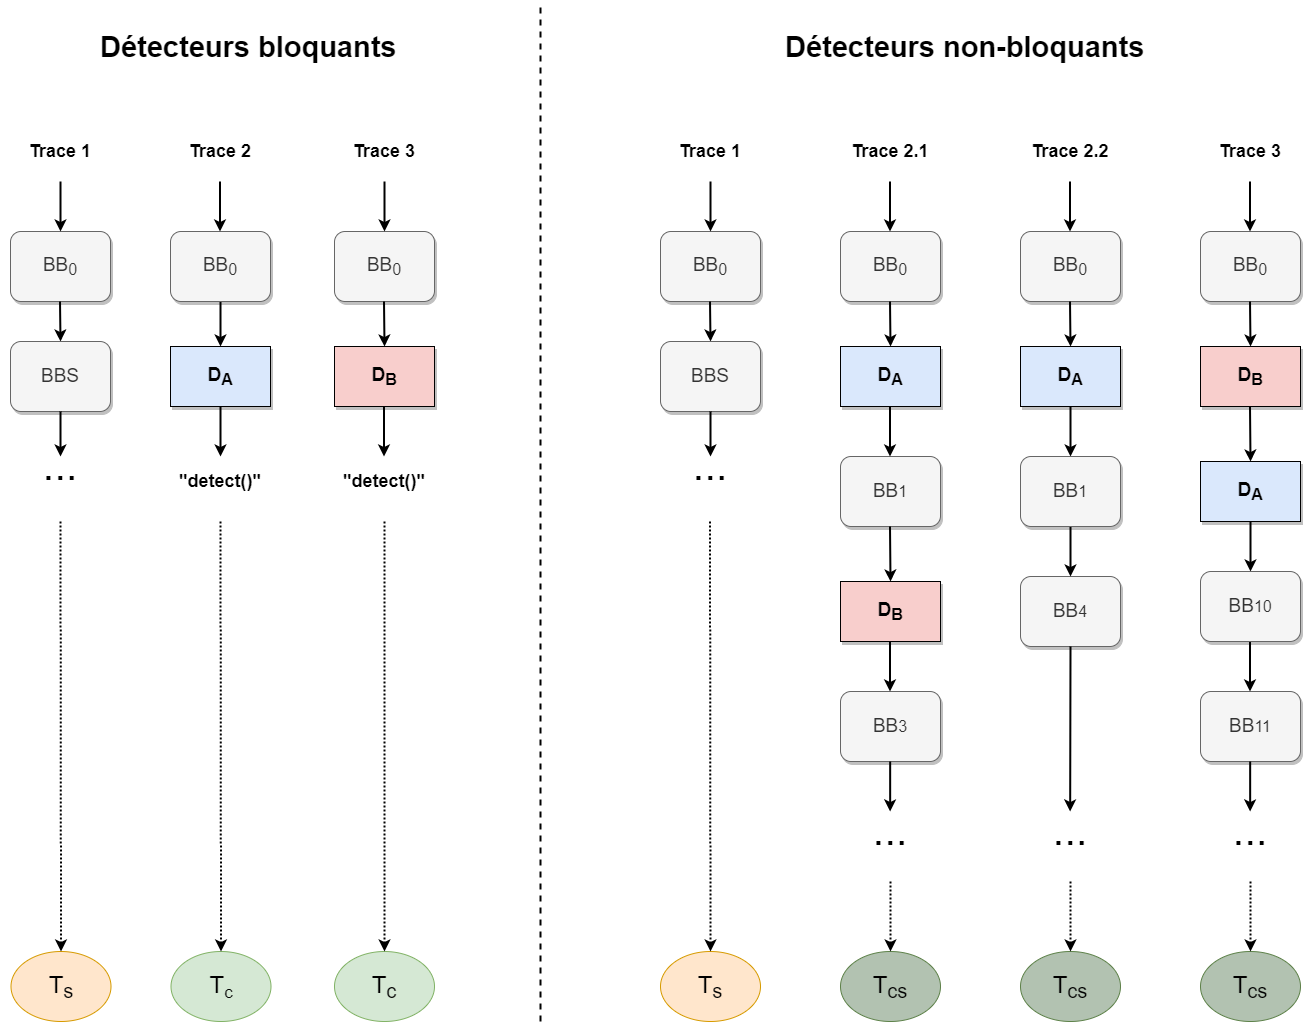
\includegraphics[scale=0.3]{ch6-ccpo/img/CCP-prop-stopping2.png}
                \caption{Exemples de traces avec détecteurs bloquants (à gauche) et non bloquants (à droite)}
                \label{fig:stop-not-to-stop}
            \end{figure}
            
        \subsection{Problématique de la couverture de $T_{cs}^{nb}(P, M)$} 
        \label{sec:ch6:valid-problematic}
        
            Dans la figure \ref{fig:stop-not-to-stop} précédente, on constate que si le détecteur $D_B$ est retiré (trace 3), alors toutes les traces d'exécution non bloquantes sont couvertes (définition \ref{def:valid}) par le détecteur $D_A$ (à l'exception de la trace 1 qui n'est de toute façon bloquée par aucun détecteur). En revanche, si on retire le détecteur $D_A$, alors il existe un chemin supplémentaire (trace 2.2) qui ne sera pas bloqué, le programme $P_{D_B}$ introduit donc au moins une nouvelle attaque par rapport aux programmes $P_{D_A, D_B}$ et $P_{D_A}$. L'ensemble de détecteurs optimal sera donc dans cet exemple $\{ D_A \}$. 
   
            \begin{defi} 
                \label{def:valid}
                Soit $Det(t)$ l'ensemble des détecteurs déclenchés dans une trace d'exécution $t$.
                Un ensemble de détecteurs $\mathcal{D}_i$ couvre un ensemble de traces $\mathcal{T}$ si chaque trace de $\mathcal{T}$ contient le déclenchement d'au moins un détecteur de $\mathcal{D}_i$:  
            \begin{equation*}
                Couvre(\mathcal{D}_i, \mathcal{T}) \equiv  t \in \mathcal{T} \mid \exists d \in \mathcal{D}_i  \mid  d \in Det(t)
            \end{equation*}                 
            \end{defi} 
            
            L'objectif étant de ne pas introduire de chemins d'attaques réussies, on s'intéresse aux attaques réussies et détectées (noté $T_{cs}(P, M)$).   
            Dans le cadre d'une exécution non bloquante, une attaque détectée termine en contre-mesure. 
            La notion d'attaque réussie pour des traces non bloquantes a du sens puisqu'on s'autorise à continuer après le déclenchement d'un détecteur afin de vérifier si l'objectif d'attaque aurait été validé dans le cas où les détecteurs ne seraient pas présents.                            
            Ainsi, les ensembles de détecteurs qui n'introduisent pas de nouvelles attaques sont ceux qui couvrent l'ensemble des traces d'attaques \textit{détectées et réussies} d'une exécution non bloquante (noté $T_{cs}^{nb}(P, M)$).
            La problématique \ref{probl:detector-optimization} revient donc à répondre à la problématique \ref{probl:detector-selection}, qui est un problème d'optimisation\footnote{La recherche de ces ensembles de détecteurs qui couvrent un ensemble de trace se rapproche de l'algorithme \textit{bloc-opt} évoqué dans le chapitre \ref{chpt:placement}.}.   

            \begin{probl}
                \label{probl:detector-selection}
                Trouver les ensembles $\mathcal{D}_i$ de détecteurs minimaux tels que chaque trace d'attaques détectées et réussies $T^{nb}_{cs}(P, M)$, pour un programme $P$ et un modèle d'attaquant $M$, soit couverte par au moins un détecteur de $\mathcal{D}_i$.
                Les ensembles minimaux sont ceux qui minimisent la fonction $\mathcal{W}(\mathcal{D})$ choisie par l'utilisateur.
            \end{probl}

            Pour la suite de cette section \ref{sec:ch6:ccpo}, on posera $\mathcal{T} = T^{nb}_{cs}(P, M)$.
            La recherche des ensembles $\mathcal{D}_i$ minimaux qui couvrent l'ensemble de trace $\mathcal{T}$ est réalisée en deux étapes:
            \begin{itemize}
                \item L'étape de classification (section \ref{sec:ch6:classification}) effectue une première passe sur les traces d'entrées afin de réduire l'espace de recherche.
                \item L'étape de sélection (section \ref{sec:ch6:selection}) consiste en la recherche des ensembles $\mathcal{D}_i$ optimaux  sur cet espace réduit.
            \end{itemize}
         
        \subsection{Classification des détecteurs}    
        \label{sec:ch6:classification}

            L'étape de classification consiste à faire un premier tri des traces d'entrées dans $\mathcal{T}$ pour trouver les détecteurs qui sont:
            \begin{itemize}
                \item \textit{inactifs}: ne se déclenchent jamais dans $\mathcal{T}$ et peuvent donc être écartés des ensembles minimaux.
                \item \textit{nécessaires}: se déclenchent au moins une fois seuls dans une trace d'exécution de $\mathcal{T}$ (sans qu'un autre détecteur ne soit déclenché), et doivent donc être conservés pour ne pas introduire de nouvelles attaques.
            \end{itemize}
            
            Tous les autres détecteurs sont dit \textit{répétitifs} et c'est sur ceux-ci qu'il faut effectuer la recherche d'ensembles minimaux.
            L'étape de \textit{classification} réduit l'espace d'exploration de la sélection des ensembles minimaux.
            En effet, seuls les détecteurs \textit{répétitifs} $\mathcal{D}_R$ doivent être considérés et seules les traces contenant uniquement des détecteurs répétitifs $\mathcal{T}_R$ (définition \ref{eq:tr}) doivent être couvertes (les traces contenant au moins un détecteur nécessaire seront de toute façon couvertes). 

            \begin{defi}[Ensemble des traces contenant uniquement des répétitifs]
                \label{eq:tr}
                \begin{equation*}
                    \mathcal{T}_{R} \equiv \forall t \in \mathcal{T} \mid Det(t) \cup \mathcal{D}_R
                \end{equation*}  
            \end{defi}
            
            La table \ref{tbl:vp-td-ccpa-classification} présente la classification des détecteurs du programme $vp2c+TD$ pour une limite de fautes jusqu'à 4\footnote{Cet exemple n'est pas étudié avec des entrées symboliques mais avec des tableaux d'entrées fixés.}. Les détecteurs peuvent être nécessaires ({\color{green!50} N}), répétitifs ({\color{orange!80} R}) ou inactifs ({\color{red!80} I}).
            
            \begin{table}[H]
            \centering
                \begin{tabular}{|l|c|c|c|c|c|c|c|c|c|c|c|}
                \hline
                \rowcolor[HTML]{EFEFEF} 
                Détecteur & $D_0$ & $D_1$ & $D_2$ & $D_3$ & $D_4$ & $D_5$ & $D_6$ & $D_7$ & $D_8$ & $D_9$ & $D_{10}$ \\ \hline
                \rowcolor[HTML]{FFCCC9} 
                \cellcolor[HTML]{EFEFEF}1 faute & I & I & I & \cellcolor[HTML]{FFCC67}R & I & I & I & I & \cellcolor[HTML]{9AFF99}N & I & \cellcolor[HTML]{FFCC67}R \\ \hline
                \rowcolor[HTML]{FFCC67} 
                \cellcolor[HTML]{EFEFEF}2 fautes & R & \cellcolor[HTML]{FFCCC9}I & R & R & R & R & R & R & \cellcolor[HTML]{9AFF99}N & \cellcolor[HTML]{FFCCC9}I & \cellcolor[HTML]{9AFF99}N \\ \hline
                \rowcolor[HTML]{9AFF99} 
                \cellcolor[HTML]{EFEFEF}3 fautes & N & \cellcolor[HTML]{FFCCC9}I & N & N & N & N & \cellcolor[HTML]{FFCC67}R & N & N & \cellcolor[HTML]{FFCCC9}I & N \\ \hline
                \rowcolor[HTML]{9AFF99} 
                \cellcolor[HTML]{EFEFEF}4 fautes & N & \cellcolor[HTML]{FFCCC9}I & N & N & N & N & \cellcolor[HTML]{FFCC67}R & N & N & \cellcolor[HTML]{FFCCC9}I & N \\ \hline
                \end{tabular}
            \caption{Classification des détecteurs pour $vp2c+TD$ en fonction du nombre d'inversion de test maximum}
            \label{tbl:vp-td-ccpa-classification}
            \end{table}
                
            Les détecteurs $D_1$ et $D_9$ sont inactifs quel que soit le nombre de fautes, ce qui s'explique par le fait qu'ils protègent des branches qui n'ont pas d'impact sur l'objectif d'attaque (respectivement ligne 12 et 18 de la fonction \texttt{verify\_pin} du listing \ref{lst:ch6:vp4-vp}). A l'inverse, le détecteur $D_8$ est nécessaire même en faute unique, étant donné que l'inversion de l'appel à la fonction \texttt{compare} permet de gagner en une faute.
            
        \subsection{Sélection des détecteurs}
        \label{sec:ch6:selection} 

            La seconde étape de la méthodologie consiste à chercher les ensembles de détecteurs répétitifs $\mathcal{D}_{Ri}$ qui, associés aux détecteurs nécessaires $\mathcal{D}_N$, couvrent l'ensemble des traces de $\mathcal{T}_R$. 
            La recherche des $\mathcal{D}_{Ri}$ optimaux est ainsi un problème d'optimisation, dont l'implémentation sera précisée dans la section \ref{sec:ccpo-impl}.

            Dans le cas de l'exemple $vp2+TD$ en deux fautes, seules deux traces d'attaques détectées réussies contiennent uniquement des détecteurs répétitifs, notées $a_1$ et $a_2$.
            Les figures \ref{tbl:trace-o1.19} et \ref{tbl:trace-o2.32} présentent respectivement l'attaque $a_1$ en une faute et l'attaque $a_2$ en deux fautes, sans prendre en compte les transitions qui ne sont pas des fautes ou des détections.
            Deux ensembles de détecteurs répétitifs $\{ D_3 \}$ et $\{ D_7 \}$ permettent de couvrir $\mathcal{T}_R = \{ a_1, a_2 \}$, et doivent être associés aux détecteurs nécessaires $\mathcal{D}_N = \{D_{8}, D_{10}\}$ pour couvrir $\mathcal{T}$:
            \begin{itemize}
                \item $\mathcal{D}_1 = \{D_3, D_8, D_{10}\}$
                \item $\mathcal{D}_2 = \{D_7, D_8, D_{10}\}$
            \end{itemize}
             
            \begin{table}[ht]
            \centering                
                \begin{tabular}{|
                >{\columncolor[HTML]{C0C0C0}}c |
                >{\columncolor[HTML]{ECF4FF}}c |
                >{\columncolor[HTML]{ECF4FF}}l |
                >{\columncolor[HTML]{FFCCC9}}c |
                >{\columncolor[HTML]{ECF4FF}}l |
                >{\columncolor[HTML]{CBCEFB}}c |
                >{\columncolor[HTML]{ECF4FF}}c |
                >{\columncolor[HTML]{CBCEFB}}c |
                >{\columncolor[HTML]{ECF4FF}}c |}
                \hline
                Trace $a_1$ & \multicolumn{2}{c|}{\cellcolor[HTML]{ECF4FF}...} & Faute (bb2) & ... & Dét 3 & ... & Dét 7 & ... \\ \hline
                \end{tabular}
            \caption{Trace de l'attaque réussie détectée $a_1$ \label{tbl:trace-o1.19}}
            \end{table}
                                
            \begin{table}[ht]
            \centering
                \begin{tabular}{|
                >{\columncolor[HTML]{C0C0C0}}c |
                >{\columncolor[HTML]{ECF4FF}}c |
                >{\columncolor[HTML]{ECF4FF}}l |
                >{\columncolor[HTML]{FFCCC9}}c |
                >{\columncolor[HTML]{ECF4FF}}l |
                >{\columncolor[HTML]{CBCEFB}}c |
                >{\columncolor[HTML]{ECF4FF}}c |
                >{\columncolor[HTML]{FFCCC9}}l |
                >{\columncolor[HTML]{ECF4FF}}c |
                >{\columncolor[HTML]{CBCEFB}}c |
                >{\columncolor[HTML]{ECF4FF}}c |}
                \hline
                Trace $a_2$ & \multicolumn{2}{c|}{\cellcolor[HTML]{ECF4FF}...} & Faute (bb2) & ... & Dét 3 & ... & Faute (bb3) & ... & Dét 7 & ... \\ \hline
                \end{tabular}
            \caption{Trace de l'attaque réussie détectée $a_2$ \label{tbl:trace-o2.32}}
            \end{table}
        
            En fonction de la pondération $\mathcal{W}$ choisie, $\mathcal{D}_{1}$ ou $\mathcal{D}_{2}$ seront sélectionnés. 
            Pour une pondération égale pour chaque détecteur, $\mathcal{D}_{1}$ et $\mathcal{D}_{2}$ sont équivalents, mais le détecteur $D_3$ correspond à la duplication de la branche fausse du test \texttt{i < size} dans la boucle et pourrait par conséquent être considéré comme plus coûteux que le détecteur $D_7$ (duplication de $D_{10}$, hors de la boucle), privilégiant ainsi l'ensemble $\mathcal{D}_{2}$.  
            Les listing \ref{lst:ch6:vp4-vp-res} et \ref{lst:ch6:vp4-compare-res} présentent les parties du code retirées (en {\color{Red}rouge}) et conservées (en {\color{OliveGreen}vert}) pour l'ensemble $\mathcal{D}_{1}$, pour respectivement les fonctions \texttt{verify\_pin} et \texttt{compare}. Le corps de contre-mesure (ici chaque variable locale $c_i$ associée à des détecteurs retirés) est également retiré.

        \subsection{Conclusion}
        \label{sec:ch6:pres-conclusion} 
                 
            La méthodologie de calcul de l'ensemble de détecteurs minimaux est ainsi découpée en deux étapes, la \textit{classification} et la \textit{sélection}, comme le montre la figure \ref{fig:ccpo-scheme}.            
            Ainsi, une seule exploration des exécutions est effectuée sur le programme $P$ contenant tous les détecteurs. Cette méthodologie impose cependant que l'évaluation de la condition d'un détecteur n'ait pas d'effet de bord sur l'exécution de la suite du programme ainsi que sur l'objectif d'attaque étudié. 
            La correction de cette approche, correspondant à la garantie qu'aucune nouvelle attaque n'est introduite par le retrait des détecteurs, est discutée en section \ref{sec:ccpo-formalisation}.
               
            \begin{figure}[!ht]\centering
                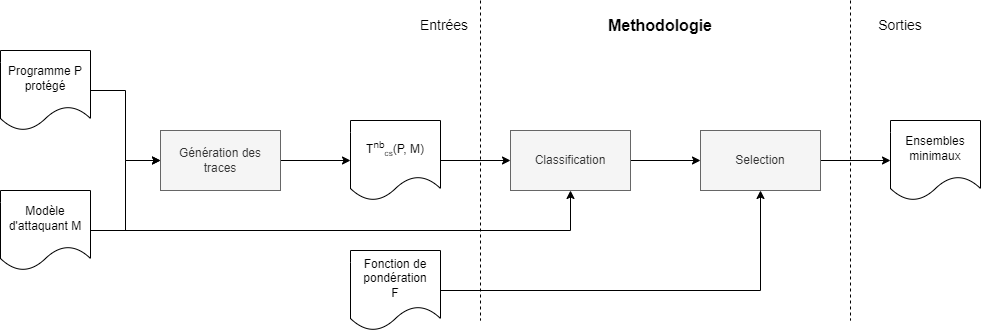
\includegraphics[scale=0.4]{ch6-ccpo/img/ccpo-scheme-select.drawio.png}
                \caption{Schéma de la méthodologie d'optimisation de détecteurs}
                \label{fig:ccpo-scheme}
            \end{figure}
    
            La problématique de l'optimisation des contre-mesures a été abordée dans les chapitres précédents et la méthodologie présentée dans ce chapitre propose une solution dans le cas des contre-mesures à détecteurs, visant à répondre à la problématique \ref{probl:detector-optimization}.
            L'optimisation de détecteurs est une forme de comparaison de programmes protégés puisqu'il s'agit de comparer les différentes variations $\mathcal{V}(P)$.            
            Elle peut aussi être utilisée en amont du processus de développement lors de l'application des contres-mesures pour aider au placement de ces contre-mesures.        
    
            La méthodologie présentée ici garantit que les détecteurs peuvent être retirés sans introduire de nouvelles attaques. Néanmoins, déterminer quelles portions du \textit{corps de contre-mesure} peuvent être enlevées par rapport à l'ensemble de détecteurs calculé n'est pas trivial dans le cas général.
            La figure \ref{fig:ccpo-metho} présente les différents cas d'utilisation de la méthodologie en fonction de la méthode de placement utilisée pour le programme $P$ : placement automatique (a) ou placement manuel (b).
            Le scénario (a) correspond au cas où le placement est effectué à l'aide d'un outil automatique, que ce soit par un outil dédié \cite{lalande} ou un compilateur \cite{Reis/ISCCO05, Proy/TACO17}.
            Il s'agit ici du scénario de l'exemple $vp2c+TD$ où la duplication de test peut être appliquée avec une granularité de l'ordre du point d'injection. 
            Dans ce cas, le programme protégé $P'$ est simplement régénéré à partir d'un ensemble de détecteurs calculé par l'algorithme d'optimisation : 
            \begin{enumerate}
                \item Appliquer systématiquement les contre-mesures.
                \item Calculer un ensemble optimal de détecteurs $D_i$.
                \item Appliquer le placement avec les détecteurs de $D_i$ uniquement.
            \end{enumerate}
    
            \begin{figure}[!ht]
            \centering
                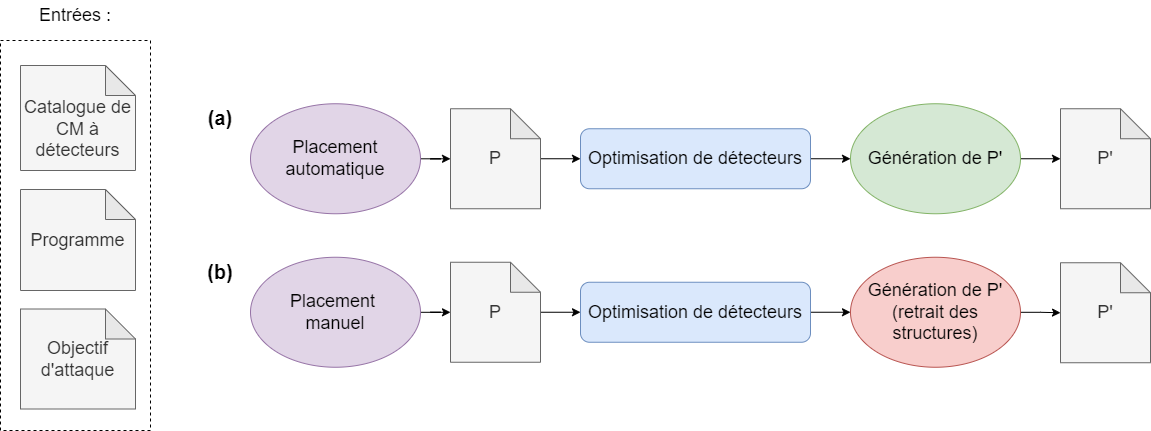
\includegraphics[scale=0.33]{ch6-ccpo/img/placement-ccpo2.drawio.png}
                \caption{Différentes applications de la méthodologie}
                \label{fig:ccpo-metho}
            \end{figure}
    
            Le scénario (b) décrit le cas où il n'est pas possible de ré-appliquer automatiquement la contre-mesure à l'aide de l'ensemble $D_i$. Cela implique qu'il faut calculer le corps de contre-mesure pouvant être retiré.
            Cette analyse n'est pas triviale puisqu'elle requiert de prendre en compte toutes les fautes possibles de manière à déterminer si une portion du corps de contre-mesure est nécessaire.
            Cette partie de la problématique n'est pas traitée dans ce manuscrit.
    
            Un dernier cas d'utilisation peut être noté et correspond à un cas particulier du scénario a, où le placement automatique est un placement \textit{optimal} (comme décrit dans le chapitre précédent). Dans ce cas, la méthodologie peut être utilisée pour vérifier l'optimalité du placement, celui-ci dépendant de la complétude et correction de l'exploration des chemins d'attaques fautés\footnote{De la même manière, l'optimisation de détecteurs repose sur la complétude et la correction des chemins d'attaques détectées.}.
      
    \section{Garanties de la méthode et protection des détecteurs}
    \label{sec:ccpo-formalisation}

        Cette section s'intéresse aux garanties de la méthodologie présentée dans la section précédente, en supposant l'exploration des chemins $T^{nb}_{cs}(P, M)$ complète et correcte.
        La section \ref{sec:exec-classification} revient sur les différentes classes d'exécution dans le cadre d'une exécution avec détecteurs non bloquants et la section \ref{sec:ccpo-rob-preserv} indique les relations autorisées entre ces classes pour préserver la robustesse du programme $P'$.
        La section \ref{sec:ccpo-trace-match} explique comment les traces d'attaques peuvent être mises en correspondance avec les traces d'attaques des différentes variations du programme $P$, permettant ainsi de vérifier que les attaques détectées dans $P$ resteront détectées dans le programme $P'$.
        Enfin, la section \ref{sec:ccpo-prot-det} s'intéresse aux possibles faux positifs et présente une solution appelée \og protection des détecteurs \fg{}. 
        
        \subsection{Classification des exécutions pour $T^{nb}(P, M)$}
        \label{sec:exec-classification}
    
            Les exécutions d'un programme peuvent être caractérisées par:
            \begin{itemize}
                \item la validation ou non de l'objectif d'attaque $\phi$.
                \item la terminaison (exécution terminée ou timeout/boucle infinie).
                \item la présence ou non de fautes.
                \item le déclenchement d'une contre-mesure (d'un détecteur).
            \end{itemize}
            
            Si on choisit d'abstraire la terminaison dans l'objectif d'attaque, ainsi que les cas d'erreurs (crash, division par zéro, accès mémoire invalide), cela permet de simplifier les catégories de traces en laissant l'utilisateur définir, dans l'objectif d'attaque, s'il considère un timeout ou une double désallocation avec \texttt{free} par exemple, comme une attaque réussie.
            C'est ce qui est fait dans Lazart, dans lequel l'utilisateur peut paramétrer les types de terminaison correspondant à une attaque réussie (voir section \ref{sec:lazart-aa}).
            
            Classiquement, les exécutions ou les traces d'exécutions, pour un programme $P$ et un modèle de faute $M$, sont partitionnées dans les ensembles suivants :
            \begin{itemize}
                \item $T_n(P, M)$: les exécutions nominales (sans fautes).
                \item $T_c(P, M)$: les attaques terminant en contre-mesure (détectées).
                \item $T_s(P, M)$: les attaques réussies ($\phi$ satisfait) et non détectées.
                \item $T_f(P, M)$: les attaques non réussies ($\phi$ non satisfait) et non détectées.
            \end{itemize}
            
            Dans le cas d'une analyse avec détecteurs non bloquants, l'exécution ne peut plus terminer en contre-mesure. 
            Pour autant il est possible de différencier les traces contenant le déclenchement d'un détecteur et celles n'en contenant pas.
            De plus, il est possible d'évaluer la condition de succès de l'objectif d'attaque, l'exécution n'étant plus interrompue par les détecteurs.
            Pour une exécution non bloquante, les traces produites à partir de $T_c(P, M)$ peuvent se décomposer en:
            \begin{itemize}
                \item $T_{cs}(P, M)$: les attaques dans lesquelles au moins un détecteur a été déclenché et où l'objectif d'attaque $\phi$ est validé.
                \item $T_{cf}(P, M)$: les attaques dans lesquelles au moins un détecteur a été déclenché et où $\phi$ n'est pas satisfait.
            \end{itemize}
       
            \begin{table}[h]
            \centering
                \begin{tabular}{|l|l|l|l|l}
                \cline{1-4}
                Ensemble / Caractéristique & $\phi$ & fautes & détecteurs                                                                                                                                                                               &  \\ \cline{1-4}
                $T_n(P, M)$                   & faux\footnotemark    & 0      & 0\footnotemark &  \\ \cline{1-4}
                $T_s(P, M)$                   & vrai   & 1+     & 0                                                                                                                                                                                        &  \\ \cline{1-4}
                $T_{cs}(P, M)$                & vrai   & 1+     & 1+                                                                                                                                                                                       &  \\ \cline{1-4}
                $T_{cf}(P, M)$                & faux   & 1+     & 1+                                                                                                                                                                                       &  \\ \cline{1-4}
                $T_f(P, M)$                   & faux   & 1+     & 0                                                                                                                                                                                        &  \\ \cline{1-4}
                \end{tabular}
            \caption{Caractéristiques des différents ensembles de traces d'exécution\label{tbl:traces-categories}}
            \end{table}

            \footnotetext[7]{On suppose que l'objectif d'attaque ne peut pas être validé dans une exécution nominale.}
            \footnotetext[8]{On suppose que les détecteurs ne se déclenchent pas dans une exécution nominale, la contre-mesure préservant le comportement observable du programme en l'absence de faute.}

            La table \ref{tbl:traces-categories} présente les caractéristiques (nombre de fautes, validation de l'objectif d'attaque et nombre de déclencheurs déclenchés) pour les cinq classes de traces d'exécution, ces ensembles de traces étant disjoints.
            
        \subsection{Préservation de la robustesse}
        \label{sec:ccpo-rob-preserv}

            Le paradoxe de dilution \cite{Dureuil/Phd16}, énoncé dans le chapitre précédent, explique qu'il soit difficile de comparer les attaques de différentes versions protégées d'un programme. Les contre-mesures ajoutent des chemins d'exécution et de la surface d'attaque.
            S'il est possible d'associer chaque trace d'exécution d'un programme $P$ à des traces d'un programme $P'$ à l'aide d'une fonction $\delta$, alors pour que $P'$ soit au moins aussi robuste que $P$, il faut que chacune des traces qui ne sont pas des attaques réussies pour $P$ restent inefficaces (attaques bloquées ou objectif d'attaque non réussi) pour $P'$. La table \ref{tbl:trace-class-changes-nb} présente les classes autorisées pour les traces de $T(P')$ en fonction des traces correspondantes (par une fonction $\delta$) dans $T(P)$ pour une conservation de la robustesse.
                                
            \begin{table}[h]
            \centering
                \begin{tabular}{|l|ccccc|}
                \hline
                \multicolumn{1}{|c|}{\multirow{2}{*}{Classe de $t \in T(P)$}} & \multicolumn{5}{c|}{Classes autorisées pour $t' \in \delta(t)$}                                                                                                                              \\ \cline{2-6} 
                \multicolumn{1}{|c|}{}                                        & \multicolumn{1}{l|}{$T_n(P', M)$} & \multicolumn{1}{l|}{$T_s(P', M)$} & \multicolumn{1}{l|}{$T_{cs}(P', M)$} & \multicolumn{1}{l|}{$T_{cf}(P', M)$} & \multicolumn{1}{l|}{$T_f(P', M)$} \\ \hline
                $T_n(P, M)$                                                   & \multicolumn{1}{c|}{\checkmark}   & \multicolumn{1}{c|}{\xmark}       & \multicolumn{1}{c|}{\checkmark}      & \multicolumn{1}{c|}{\checkmark}      & \checkmark                        \\ \hline
                $T_s(P, M)$                                                   & \multicolumn{1}{c|}{\checkmark}   & \multicolumn{1}{c|}{\checkmark}   & \multicolumn{1}{c|}{\checkmark}      & \multicolumn{1}{c|}{\checkmark}      & \checkmark                        \\ \hline
                $T_{cs}(P, M)$                                                & \multicolumn{1}{c|}{\checkmark}   & \multicolumn{1}{c|}{\xmark}       & \multicolumn{1}{c|}{\checkmark}      & \multicolumn{1}{c|}{\checkmark}      & \checkmark                        \\ \hline
                $T_{cf}(P, M)$                                                & \multicolumn{1}{c|}{\checkmark}   & \multicolumn{1}{c|}{\xmark}       & \multicolumn{1}{c|}{\checkmark}      & \multicolumn{1}{c|}{\checkmark}      & \checkmark                        \\ \hline
                $T_f(P, M)$                                                   & \multicolumn{1}{c|}{\checkmark}   & \multicolumn{1}{c|}{\xmark}       & \multicolumn{1}{c|}{\checkmark}      & \multicolumn{1}{c|}{\checkmark}      & \checkmark                        \\ \hline
                \end{tabular}
            \caption{Classes autorisées pour les traces $t' \in f(t)$ \label{tbl:trace-class-changes-nb}}
            \end{table}
            
            L'optimisation de détecteurs implique qu'un programme $P'$ puisse avoir des attaques réussies (non détectées) nécessitant moins de fautes que leur attaque correspondante dans $P$, c'est-à-dire $|F(t')| < |F(t)|, t \in T_s(P, M), t' \in T_s(P', M), t' \in \delta(t)$ (avec $F(t)$ la liste ordonnée des fautes dans la trace $t$). 

        \subsection{Correspondances entre les traces}          
        \label{sec:ccpo-trace-match}
            
            \begin{figure}[htbp]
            \centering
                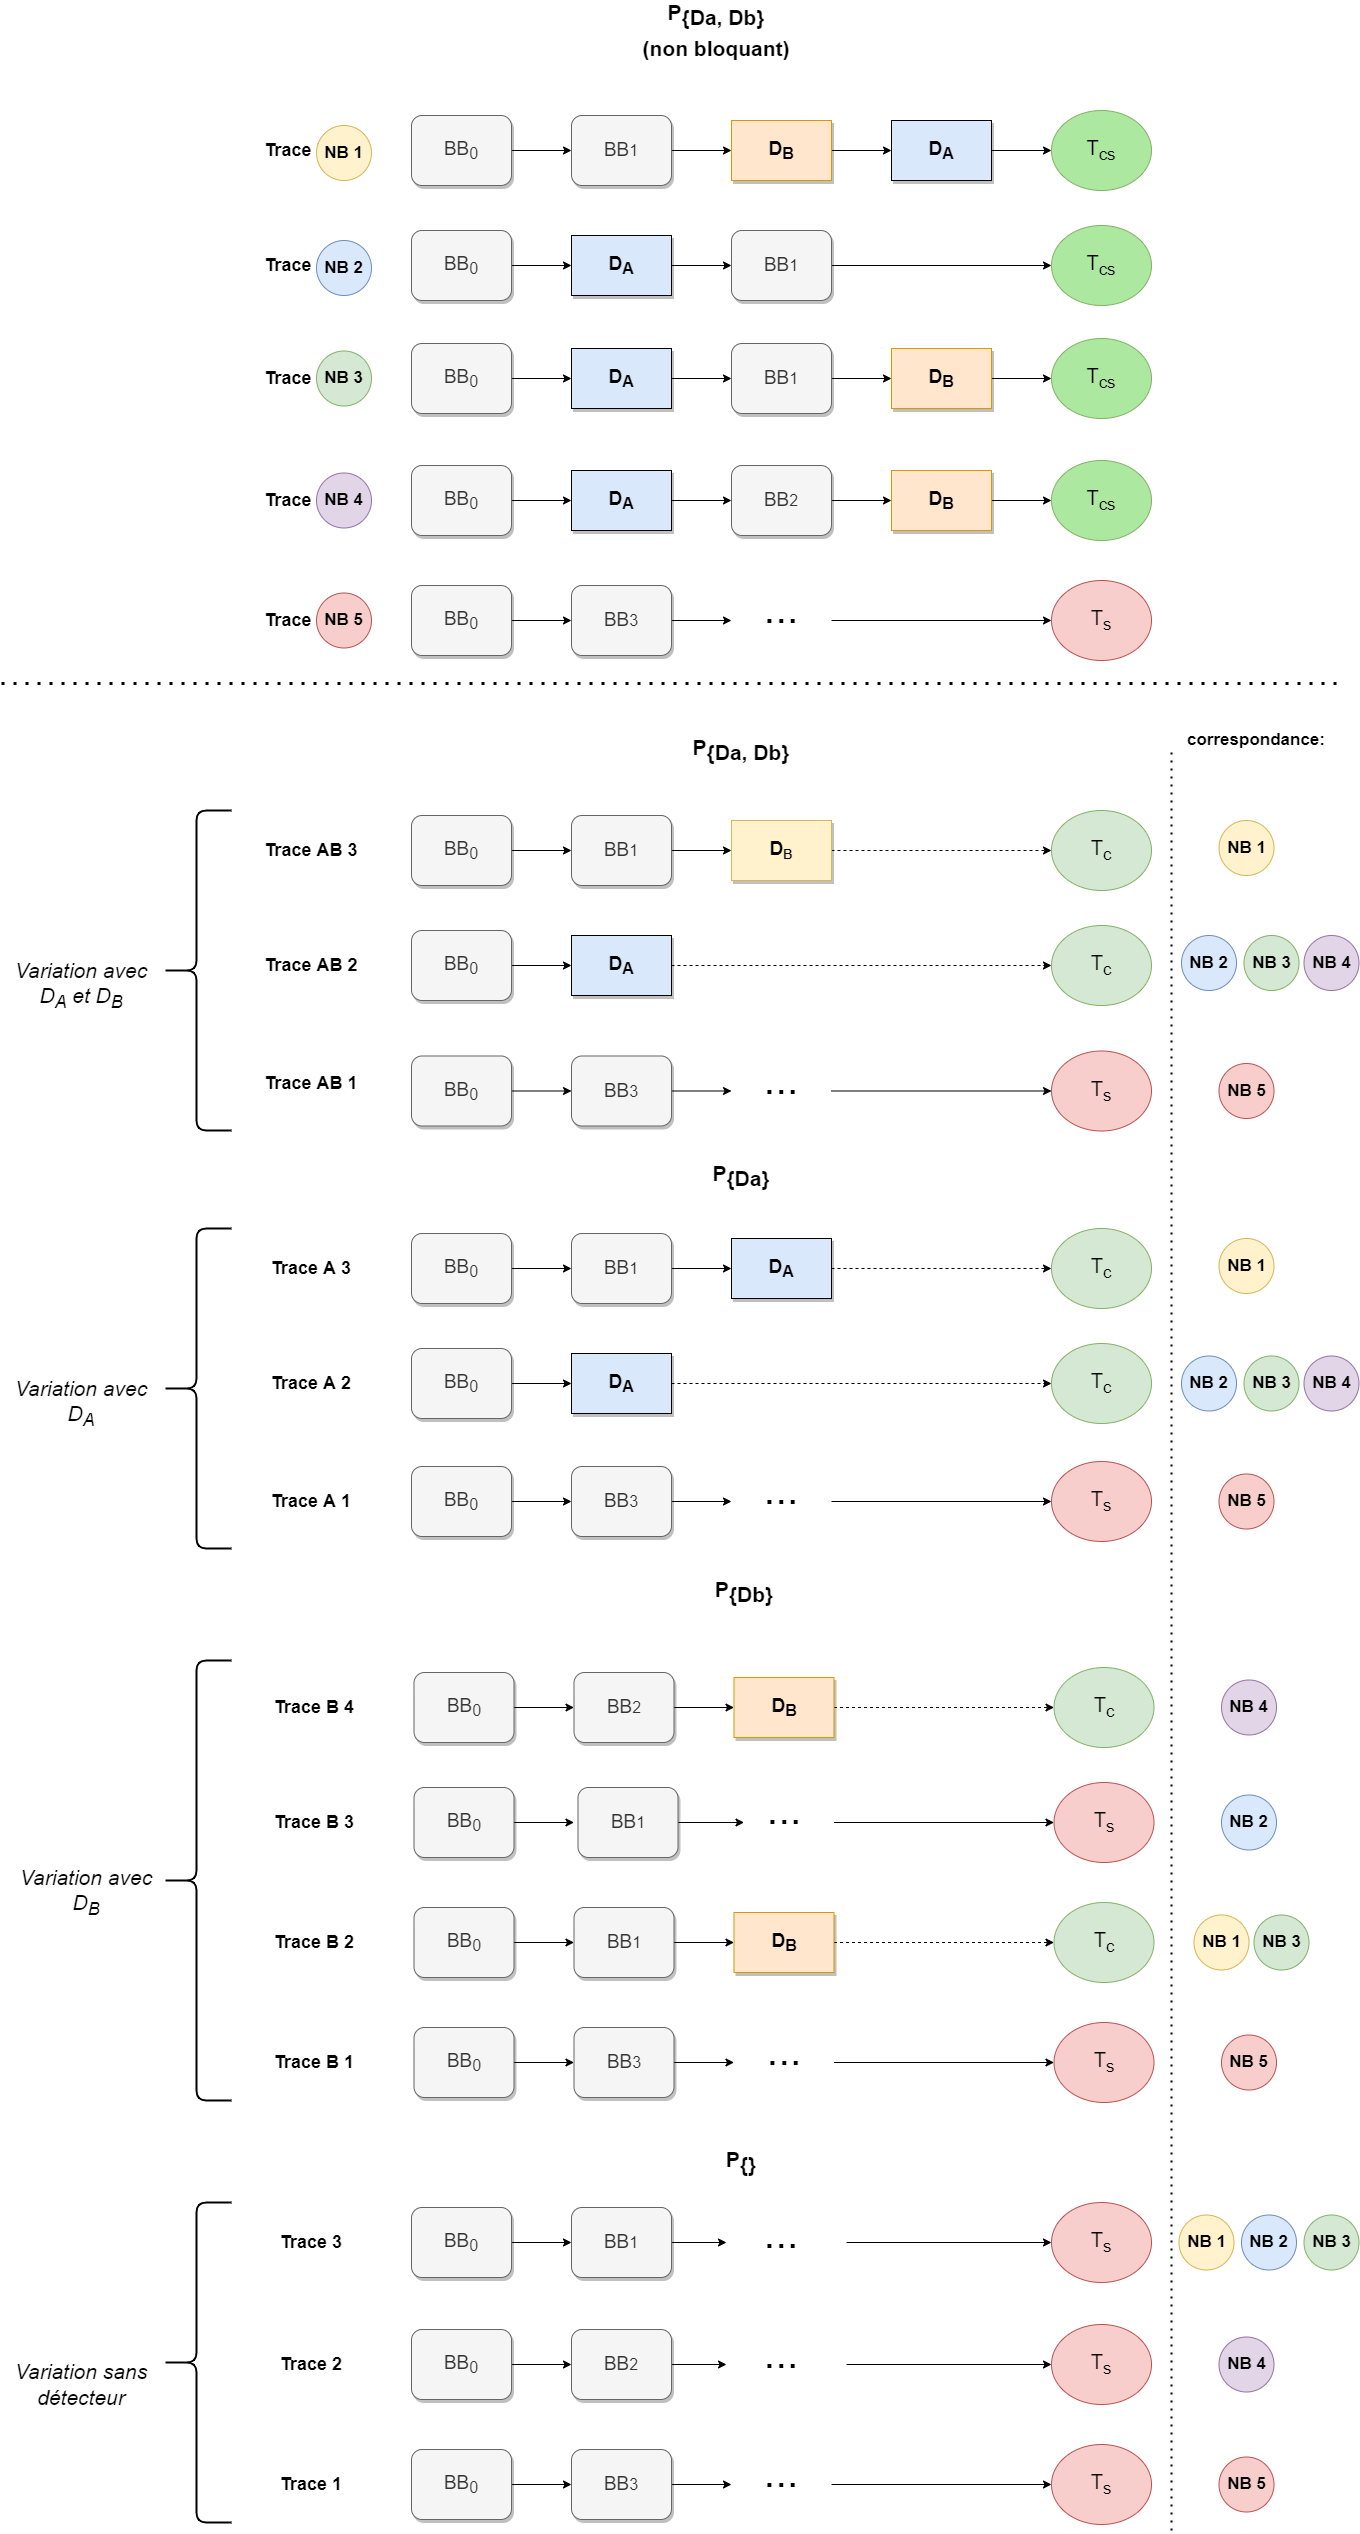
\includegraphics[scale=0.27]{ch6-ccpo/img/trace-corresp.drawio.png}
            \caption{Exemple de correspondance entre les traces des différentes variations $\mathcal{V}(P)$}
            \label{fig:ch6:trace-corresp}
            \end{figure}

            Cette section vise à établir les correspondances entre les traces d'attaques des différentes variations de $P$ et les traces d'exécution avec détecteurs non bloquants sur le programme $P$.     
            Une trace d'exécution bloquante peut correspondre à plusieurs traces d'exécutions non bloquantes. Dans ce cas, la trace bloquante (définition \ref{def:block-trace}) est un préfixe de chaque trace non bloquante correspondante (définition \ref{def:nonblock-trace}).
            
            \begin{defi}
                \label{def:block-trace}
                Les traces d'attaque détectée avec détecteurs bloquants $T_c(P, M)$ sont de la forme $s_0 ... s_n d_i$, avec $s_i$ les transitions nominales ou fautées et $d_i$ le déclenchement d'un détecteur.
            \end{defi}
            
            \begin{defi}
                \label{def:nonblock-trace}
                Les traces d'attaque détectée avec détecteurs non bloquants $T_{c}^{nb}(P, M)$ sont de la forme $s^1_0 ... s^1_{n_1} d_i s^2_0 ... s^2_{n_2} d_j ...$ avec $s^i_j$ les transitions nominales ou fautées et $d_i$ les déclenchements de détecteurs.
            \end{defi}
                    
            La figure \ref{fig:ch6:trace-corresp} présente les correspondances entre les traces des différentes variations d'un programme $P$ contenant deux détecteurs $D_A$ et $D_B$, et les traces de l'exécution non bloquante $T^{nb}(P)$ (en haut).
            Pour chaque trace d'exécution, sa classe peut être attaque réussie ($T_s$) ou attaque détectée ($T_c$). 
            Dans le cas de l'exécution non bloquante, les traces d'attaques réussies et détectées sont indiquées par $T_{cs}$.
            Dans cet exemple, les ensembles de détecteurs $\{D_B\}$ et $\{\}$ ne permettent pas de couvrir l'ensemble des attaques de $T^{nb}$ et les programmes $P_{D_B}$ et $P_{\{\}}$ introduisent de nouvelles attaques réussies qui ne sont pas détectées (respectivement les traces $B3$ et les traces $2$ et $3$).
            
            L'exploration des exécutions non bloquantes du programme $P$ contenant tous les détecteurs permet ainsi d'évaluer la robustesse de chaque variation de $P$.
            Si toutes les traces de $T^{nb}_{cs}{P}$ sont couvertes par (au moins) un détecteur d'un ensemble $\mathcal{D}_{i}$, alors les traces correspondante dans $P_{\mathcal{D}_{i}}$ seront détectées (dans $T_c(P_{\mathcal{D}_{i}})$).
            Cela implique cependant que les conditions des détecteurs non bloquants n'aient pas d'effet de bord sur le reste de l'exécution du programme (et l'objectif d'attaque).
                     
        \subsection{Protection des détecteurs}
        \label{sec:ccpo-prot-det}

            L'analyse de l'ensemble $T^{nb}_{cs}(P, M)$ peut néanmoins générer des faux positifs, puisqu'il existe certaines exécutions qui peuvent fausser l'analyse, en classifiant un détecteur comme \textit{nécessaire} de manière incorrecte. Il s'agit des fautes qui forcent le déclenchement d'un détecteur (alors que la condition de détection est fausse).
             
            Le problème s'illustre facilement avec le modèle d'inversion de test, où la notion de \textit{forcer le passage dans un détecteur} est plus claire.
            L'extrait de programme \ref{lst:detector-base} contient un simple détecteur avec pour condition \texttt{c}. Si l'exploration des exécutions fautées est complète, et qu'il existe des exécutions où $c$ est faux avec encore (au moins) une faute de disponible, alors il existe un ensemble d'exécutions dans lesquelles le test est inversé pour forcer l'entrée dans le détecteur.
                
\begin{minipage}{0.93\linewidth}
\lstset{escapeinside={<@}{@>}}
\lstset{caption={Exemple de trace forcant le passage en contre-mesure},label=lst:detector-base, numbers=left,xleftmargin=2em}
\begin{lstlisting}
...

if(c) {
countermeasure("X");
}

...\end{lstlisting} 
\end{minipage}

            L'ensemble de ces traces donnant lieu à une sur-approximation de la méthodologie est nommé $T^{nb}_{b}(P, M)$ et est contenu dans $T_{cs}(P, M)$. La recherche des ensembles minimaux de détecteurs doit donc s'effectuer sur $T^{nb}_{cs}(P, M) / T^{nb}_{b}(P, M)$.
            Trouver les traces $T^{nb}_b(P, M)$ à partir de $T^{nb}_{cs}(P, M)$ n'est pas trivial, mais une solution consiste à interdire les fautes forçant le passage vers la branche \textit{vraie} des détecteurs au niveau de la génération des traces. C'est cette approche qui est implémentée dans Lazart.
                
    \section{Implémentation et expérimentations}
    \label{sec:ccpo-impl}

        Cette section présente les résultats obtenus pour la méthodologie décrite dans ce chapitre et son implémentation au sein de l'outil Lazart.
        
        \subsection{Implémentation dans Lazart}
        \label{sec:ch6-impl}

            Cette section présente l'implémentation de la méthodologie d'optimisation de détecteurs au sein de Lazart.
            La section \ref{sec:ch6-non block} revient sur l'implémentation des détecteurs non bloquants. 
            Les sections \ref{sec:ch6-impl-classification} et \ref{sec:ch6-impl-selection} détaillent respectivement les étapes de classification et de sélection.
            Enfin, la section \ref{sec:ch6-supdect} discute de la problématique de la création de \textit{super-détecteur} lors de l'application automatique de certaines contre-mesures.

            \subsubsection{Détecteurs non bloquants}
            \label{sec:ch6-non block}
        
                Usuellement, les outils d'analyses considèrent la terminaison d'une exécution en contre-mesure comme un type de terminaison à part entière.                 
                Pour l'analyse de contre-mesures présentée dans ce chapitre, il est nécessaire de supporter un mode d'exécution dans lequel les détecteurs ne terminent pas l'exécution du programme, tout en gardant en mémoire les détecteurs déclenchés. 
                Le déclenchement d'un détecteur $D_i$ est traduit par un évènement de type spécifique qui est affiché sur la sortie pour être récupérée lors du rejeu (voir section \ref{sec:lazart-impl-klee-replay}).   
            
                En pratique, la fonction associée au déclenchement d'un détecteur bloquant correspond au code C présenté dans le listing \ref{lst:trigger-fct-stop}. Le paramètre \texttt{\_det\_id} correspond à l'identifiant unique du détecteur déclenché, en tant que chaîne de caractères. 
                L'exécution est arrêtée avec un appel à \texttt{klee\_assume(false);}.
    
\lstset{style=codeC, caption={Fonction de déclenchement de détecteur bloquant},label={lst:trigger-fct-stop}}
\begin{lstlisting}     
void _LZ__trigger_detector_stop(const char* _det_id)
{
    _LZ__detector_alarm_ = true;
    if(klee_is_replay())
        printf("\n[CM] triggered %s \n", _det_id);  // See wiki for print syntax.
    klee_assume(false); // Cut exploration.
}
\end{lstlisting}  

                \begin{sloppypar}
                Le listing \ref{lst:trigger-fct-nb} correspond à la fonction pour un détecteur non bloquant, qui ne diffère que par l'absence de l'appel à \texttt{klee\_assume(false);}.
                La variable globale \texttt{\_LZ\_\_detector\_alarm\_} permet de vérifier dans l'objectif d'attaque si au moins un détecteur a été déclenché. 
                La question de savoir si une attaque est détectée peut également se faire en vérifiant si $Det(t) = \emptyset$ dans l'\gls{api} Python.
                \end{sloppypar}
    
\lstset{style=codeC, caption={Fonction de déclenchement d'un détecteur non bloquant},label=lst:trigger-fct-nb}
\begin{lstlisting}     
void _LZ__trigger_detector(const char* _det_id)
{
    _LZ__detector_alarm_ = true;    
    if(klee_is_replay()) 
        printf("\n[CM] triggered %s \n", _det_id); // See wiki for print syntax.
}

\end{lstlisting}  

                Dans le cas d'une exécution symbolique complète et correcte, une analyse d'attaque avec des détecteurs bloquants ou non bloquants n'a pas d'impact sur les chemins d'attaques réussies obtenus.
                En effet, seuls des chemins d'attaques détectées peuvent être générés à partir d'un détecteur non bloquant.
                Le mode bloquant a l'avantage d'arrêter plus tôt l'exploration des attaques détectées et donc de réduire le temps de l'exploration. C'est pourquoi il s'agit du mode par défaut pour les analyses d'attaques, les détecteurs non bloquants étant réservés à l'optimisation de détecteurs.
            
            \subsubsection{Classification}
            \label{sec:ch6-impl-classification}
    
                 La première étape de classification est effectuée sur l'ensemble des traces d'attaques réussies et détectées, dans une exécution non bloquante.
                 La classification des détecteurs repose sur le calcul du \textit{niveau de répétition minimal} $L_m[D_i]$ de chaque détecteur $D_i$ sur l'ensemble des traces.              
                 Pour chaque trace, on calcule le \textit{niveau de répétition} qui correspond au nombre de détecteurs \textit{différents} déclenchés dans cette trace (c'est-à-dire sans prendre en compte les répétition d'un même détecteur au sein de la trace).
                 $L_m[D_i]$ qui est initialisé à $\infty$ et est mis à jour à chaque trace pour chaque détecteur présent.
                 Chaque détecteur est finalement classé en fonction de ce niveau de répétition minimal :
                \begin{itemize}
                    \item Inactif: si $L_m[D_i] = \infty$ \textit{(ne s'est jamais déclenché)}
                    \item Nécessaire: si $L_m[D_i] = 1$
                    \item Répétitif: si $L_m[D_i] \in \; ]1; \infty[$
                \end{itemize}
    
                L'implémentation utilise une classification en deux étapes, permettant d'obtenir les résultats pour chaque nombre de fautes jusqu'à $n$ fautes.
                Dans un premier temps, la \textit{classification locale} est calculée, correspondant au calcul de la classe de chaque détecteur pour un nombre de fautes donné.
                Dans un second temps, la classification globale est calculée, en fonction de la classification locale pour les nombres de fautes inférieurs (correspondant à une relation d'ordre $inactif < repetitif < necessaire$:
                \begin{itemize}
                    \item si un détecteur est \textit{répétitif} en $n$ fautes, il est \textit{répétitif} ou \textit{nécessaire} en $m$ fautes pour $m \geq n$.
                    \item si un détecteur est \textit{nécessaire} en $n$ fautes, il est \textit{nécessaire} en $m$ fautes pour $m \geq n$.
                \end{itemize}
                
            \subsubsection{Étape de sélection}
            \label{sec:ch6-impl-selection}
    
               Pour rappel, l'étape de sélection vise à trouver les ensembles minimaux (selon la fonction de pondération $\mathcal{W}$) de détecteurs répétitifs (dans $\mathcal{D}_R$) qui couvrent l'ensemble des traces $\mathcal{T}_R$. 
               Une première solution consiste à essayer toutes les combinaisons de détecteurs possibles, et de conserver uniquement les ensembles qui couvrent $\mathcal{T}_R$.
               
               L'algorithme présenté dans le listing \ref{lst:ch6-select} présente le pseudo code de l'algorithme de sélection utilisé dans Lazart.
               Celui-ci vise à explorer les ensembles de détecteurs contenant un seul élément (ajoutés à la pile, lignes 4 à 6) et explorer progressivement les ensembles contenant un élément de plus.
               L'ensemble des solutions minimales (\texttt{bests}) est initialisé avec l'ensemble $\mathcal{D}_r$.
               L'objectif est d'arrêter l'exploration lorsqu'un ensemble est d'ores et déjà supérieur aux minimums courants\footnote{Par exemple: si $\{D_{1}\}$ couvre l'ensemble de traces, alors $\{D_{1}, D_2\}$ le couvre aussi. Cependant l'ensemble $\{D_{1}, D_2\}$ ne peut pas être une solution minimale puisqu'il a un poids plus élevé et il n'est pas nécessaire d'explorer les ensembles plus grands. En revanche, il est nécessaire d'explorer $\{D_{2}\}$ qui pourrait faire partie des solutions minimales.} (lignes 11 et 12).
               Si un ensemble ne couvre pas $\mathcal{T}_R$ et qu'il n'a pas un poids supérieur aux ensembles minimaux déjà trouvés, alors les ensembles avec un détecteur de plus sont ajoutés à la liste des ensembles à explorer (lignes 22 à 25).

\lstset{language=python, caption={Pseudo-code de l'algorithme de sélection},label=lst:ch6-select}
\begin{lstlisting}
def selection(traces, repetitives):
bests = [repetitives] # Current best sets covering traces.

set_stack = [] # Stack of set to be checked, by total weight (W)
for det in repetitives: 
set_stack += [det] # Initialize with singletons.

while set_stack not empty:
curr = set_stack.pop()

if W(curr) > W(bests[0]):  
    continue # Stop exploration for super-sets

if Cover(curr, traces): 
    # Update best sets.
    if W(curr) == W(bests[0]):
        bests += curr
    elif W(curr) < W(bests[0]):
        bests = [curr]
        
    continue # Stop exploration for super-sets
else: # Add super-sets to stack
    for det in repetitives:
        if det not in curr:
            set_stacks.insert(curr + [det])

return bests
\end{lstlisting} 
           
                La complexité de cet algorithme est dépendante du nombre de détecteurs répétitifs $\mathcal{D}_{R}$ ainsi que du nombre de traces dans $\mathcal{T}_{R}$.
                Dans le pire cas, tous les détecteurs sont répétitifs et toutes les variations de $P$ sont explorées.
                Néanmoins, les expérimentations tendent à montrer que cette étape est souvent négligeable par rapport au reste de l'analyse (voir section \ref{sec:ch6:exp:perf}).
                Dans le pire cas, la seule solution est l'ensemble $\mathcal{D}_R$ (qui couvre toujours l'ensemble $\mathcal{T}_R$ par définition).
                Par ailleurs, l'algorithme de placement \textit{bloc-opt} (voir section \ref{sec:placement-other}) visant à obtenir la couverture d'un \gls{ip} protégé par trace d'attaques pourrait être implémenté avec cet algorithme (en cherchant des ensembles d'\gls{ip}s plutôt que des ensembles de détecteurs).
    
            \subsubsection{Application automatique et super-détecteurs}
            \label{sec:ch6-supdect}
    
                L'application de la duplication de test systématique sur un détecteur déjà existant mène à la création de structures plus complexes comme le montre la figure \ref{fig:super-detect}, ce qui est le cas dans $vp2c+TD$ sur la vérification du compteur de boucle déjà présente dans la fonction \textit{compare}.                    
       
                \begin{figure}[H]\centering
                \begin{multicols}{2}
\lstset{language=C,style=codeC, caption={},label={lst:detector-nominal}, showlines=true}
\begin{lstlisting}
...

if(cond) {
    detect("D1");
} 

...





\end{lstlisting}  
\columnbreak

\lstset{language=C,style=codeC, caption={},label={lst:detector-super}}
\begin{lstlisting}
...

if(bool c_tmp = cond) { 
    if(!c_tmp) {
        detect("DT");
    }
    detect("D1");
}
else if (c_tmp) {
    detect("DF");
}
...\end{lstlisting}  
\end{multicols}
                \caption{Détecteur (à gauche) et super-détecteur formé par $TD$ (à droite) \label{fig:super-detect}}
                \end{figure}
            
                La structure formée par le doublement de la branche du détecteur original (ligne 3 à 8) est appelée \textit{super-détecteur}. Celle-ci pose problème, puisque $D_1$ n'a plus la structure \textit{if(cond) { detect(); }} après l'application de la duplication de test.           
                Dans ce cas, la duplication est redondante par rapport au test original (c'est-à-dire que $D_1$ sera toujours déclenché si $D_T$ est déclenché).
                
                L'implémentation dans Lazart lève un avertissement lorsque l'application locale d'une contre-mesure est susceptible de générer un super-détecteur\footnote{Notez qu'il serait possible de dupliquer le test sans créer de super-détecteur, en dupliquant le test en dehors du détecteur (sans l'imbriquer). Cependant, il s'agit là d'une autre contre-mesure que la duplication de test de Lazart.}. 
                La généralisation de la méthodologie à des structures telles que les super-détecteurs fait partie des perspectives de ces travaux.

        \subsection{Expérimentations}
        \label{sec:ch6:exp}
        
            Cette section présente les résultats obtenus sur un ensemble de couples de programmes et de contre-mesures.                      
            La section \ref{sec:ch6:exp:bench} présente les différents programmes utilisés dans ces expérimentations, ainsi que les modèles d'attaquants considérés.
            La section \ref{sec:ch6:exp:cms} détaille les différentes contre-mesures qui ont été étudiées.
            La section \ref{sec:ch6:exp:results} présente le nombre de détecteurs retirés pour chaque exemple de test. La section \ref{sec:ch6:exp:phi} s'intéresse à l'impact de l'objectif d'attaque sur les résultats et la section \ref{sec:ch6:exp:perf} présente les métriques de performance obtenus.
        
            \subsubsection{Programme d'exemple}
            \label{sec:ch6:exp:bench}
        
                Les expérimentations présentées dans cette section utilisent cinq programmes:
                \begin{itemize}
                    \item $vp2c$: la version 2c du programme \textit{verify\_pin}.
                    \item $aes$ et $aes$ $rk$: une implémentation de l'algorithme de chiffrement \gls{aes} et une implémentation de l'étape \texttt{addRoundKey}.
                    \item $gc1$: une implémentation d'une fonction de génération de nonce \textit{get\_challenge}.
                    \item $fu1$: la version 1 du programme \textit{firmware\_updater}.
                \end{itemize}
            
                Chaque programme est analysé avec le modèle d'inversion de test ($TI$).
                Les programmes $vp2c$ et $fu0$ ont déjà été présentés dans le chapitre précédent et on utilisera les mêmes objectifs d'attaque.
                Le programme $gc1$ contient plusieurs contre-mesures intégrées (pile cachée, compteur de boucle) avec des détecteurs.
                Le programme $aes$ est une implémentation de l'algorithme \gls{aes} et $aes$ $rk$ ne contient que l'étape $addRoundKey$. L'objectif d'attaque est ici de ne pas générer le bon chiffré.
            
            \subsubsection{Les contre-mesures}
            \label{sec:ch6:exp:cms}
            
                En plus des détecteurs éventuellement présents dans les programmes originaux, trois contre-mesures ajoutées systématiquement seront considérées:
                \begin{itemize}
                    \item la duplication de test ($TD$) déjà présentée précédemment.
                    \item la contre-mesure SecSwift Control Flow \cite{Ferriere/LLVM19} ($SSCF$).
                    \item la contre-mesure de compteurs d'instructions niveau C \cite{lalande} ($CNT$).
                \end{itemize}
            
                \paragraph{}\textbf{SecSwift ControlFlow}. La contre-mesure \gls{SSCF} vise la protection du flot de contrôle et repose sur un système de signature par XOR.
                La figure \ref{fig:sscf-scheme} présente la protection d'un branchement à l'aide de la contre-mesure \gls{SSCF}. 
                Chaque bloc de base se voit assigné un identifiant unique et les variables \texttt{RTS} (Register Transfert Signature) et \texttt{GSR} (General Signature Register) sont utilisées pour vérifier que la bonne branche a été sélectionnée. ??? 
                \texttt{GSR} étant égal à l'identifiant du bloc courant dans une exécution nominale.
                \texttt{RTS} est préparée (premier bloc) en fonction de la condition en lui associant l'identifiant du bloc courant XOR le bloc de destination.
                Lors de l'arrivée dans le bloc de destination, la variable \texttt{GSR} est xorée avec \texttt{RTS}.
                Une assertion vérifie que \texttt{GSR} est bien égal à l'identifiant attendu, et lève une erreur dans le cas contraire. Ces assertions correspondent aux détecteurs pour \gls{SSCF}.         

                \begin{figure}[h]
                \centering
                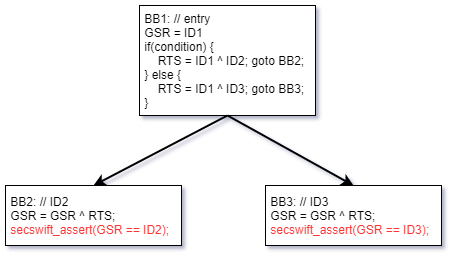
\includegraphics[width=0.55\textwidth]{ch6-ccpo/img/secswift-CF.png}
                \caption{Schéma de protection d'un branchement avec $SSCF$ \cite{Ferriere/LLVM19}}
                \label{fig:sscf-scheme}
                \end{figure}
            
                \textbf{Compteurs d'instructions}. La contre-mesure $CNT$ vise la protection contre le saut d'instruction niveau C en introduisant des compteurs incrémentés entre chaque instruction.
                Le listing \ref{lst:lalande} présente le début de la fonction \textit{verify\_pin} protégée avec $CNT$.
                Les macros \texttt{INCR} et \texttt{CHECK\_INCR} effectuent l'incrémentation d'un compteur, la seconde ajoutant un détecteur pour vérifier que celui-ci vaut bien la valeur attendue.
                Diverses macros sont proposées dans \cite{lalande} afin de protéger différentes structures (appel de fonction, boucle, condition...). La version étudiée ici est légèrement modifiée par rapport au papier original, certaines macros ajoutant un effet de bord dans la condition des détecteurs\footnote{Par exemple, la macro \texttt{CHECK\_INCR(cnt,val, det\_id) cnt = (cnt == val ? cnt + 1 : detect(det\_id));} dans sa version originale modifie le compteur dans le cas où une erreur est détectée. La vérification (détecteur) et la ré-initialisation du compteur ont donc été séparées.}.
             
\begin{minipage}{0.93\linewidth}
\lstset{escapeinside={<@}{@>}, label=lst:lalande}
\begin{lstlisting}
#define <@{\color{red!95} INCR}@>(cnt,val)  cnt = cnt + 1;
#define <@{\color{red!95} CHECK\_INCR}@>(cnt,val, cm_id) if(cnt != val) detect(cm_id); \
cnt = cnt + 1;
[...]


bool verify_pin(<@{\color{red!95}uint8\_t* CNT\_0\_VP\_1}@>) 
{
<@{\color{red!95} CHECK\_INCR(*CNT\_0\_VP\_1, CNT\_INIT\_VP + 0, 0LL)}@>
g_authenticated = 0;
<@{\color{red!95} CHECK\_INCR(*CNT\_0\_VP\_1, CNT\_INIT\_VP + 1, 1LL)}@>
<@{\color{red!95} DECL\_INIT(CNT\_0\_byteArrayCompare\_CALLNB\_1, CNT\_INIT\_BAC)}@>
<@{\color{red!95} CHECK\_INCR(*CNT\_0\_VP\_1, CNT\_INIT\_VP + 2, 2LL)}@>
bool res = byteArrayCompare(user_pin, card_pin, PIN_SIZE<@{\color{red!95}, \&CNT\_0\_compare\_CALLNB\_1}@>);
[...]
\end{lstlisting}
\end{minipage}

            \subsubsection{Détecteurs retirés}
            \label{sec:ch6:exp:results}
                
                La table \ref{tbl:ch6:exp:ccpo-all} présente les résultats obtenus pour les différents exemples.
                La colonne "Programme" indique quel programme de base est utilisé et la colonne "Contre-mesure" indique la contre-mesure systématique ajoutée ("-" indiquant qu'aucune contre-mesure n'est ajoutée). 
                La troisième colonne correspond au nombre global de détecteurs (après l'ajout de la contre-mesure).
                Les colonnes suivantes indiquent le pourcentage de détecteurs retirés après l'application de la méthodologie.
                         
                \begin{table}[htbp]
                \caption{Pourcentage de détecteurs retirés pour différents programmes}\label{tbl:ch6:exp:ccpo-all}
                \begin{center}
                \begin{tabular}{cc|c|ccc}
                    Programme & Contre-mesure & $\mathcal{D}(P)$ & 1 faute   & 2 fautes   & 3 fautes   \\
                    \hline
                    \hline
                    vp2c       & TD            & 11         & 72\% & 63\% & 18\% \\
                    vp2c       & SSCF          & 13         & 92\% & 76\% & 23\% \\
                    vp2c       & CNT           & 31         & 93\% & 93\% & 32\% \\
                    \hline
                    fu0       & TD            & 14         & 0\%  & 0\%  & 0\%  \\
                    fu0       & SSCF          & 24         & 12\% & 12\% & 8\%  \\
                    \hline
                    gc1       & -             & 11         & 81\% & 72\% & 63\% \\
                    gc1       & TD            & 39         & 37\% & 34\% & 34\% \\
                    gc1       & SSCF          & 38         & 57\% & 28\% & 28\% \\
                    \hline
                    aes rk    & TD            & 2          & 50\% & 50\% & 0\%  \\
                    aes rk    & SSCF          & 3          & 66\% & 33\% & 0\%  \\
                    \hline
                    aes c     & TD            & 8          & 50\% & 50\% & 0\%  \\
                    aes c     & SSCF          & 13         & 76\% & 61\% & 38\%
                    \end{tabular}
                \end{center}
                \end{table} 
                        
                On constate que le nombre de détecteurs retirés dépend fortement du programme et de la contre-mesure considérée. Naturellement, plus la limite de fautes est élevée, plus les détecteurs sont nécessaires.
                L'exemple $vp2c + CNT$ est un cas où la contre-mesure n'est pas prévue pour le modèle de faute considéré ($CNT$ visant la protection contre les sauts d'instruction au niveau C), ce qui explique pourquoi autant de détecteurs peuvent être retirés (jusqu'à 2 fautes).
                Dans certains exemples (tels que $fu0 + TD$ ou bien $aes$ $rk$ en 3 fautes), il n'est simplement pas possible de retirer de détecteurs.
                
            \subsubsection{Impact de l'objectif d'attaque}
            \label{sec:ch6:exp:phi}
        
                La table \ref{tbl:ch6:exp:vp-td-phi} présente les résultats obtenus sur l'exemple $vp2c$, en fonction de l'objectif d'attaque considéré: $\phi_{auth}$ (s'authentifier malgré un PIN incorrect), $\phi_{ptc}$ (ne pas décrémenter le compteur d'essais), leurs disjonction et conjonction logiques ($\phi_{auth\; \vee \;ptc}$ et $\phi_{auth\; \wedge \;ptc}$), ainsi que l'objectif d'attaque $\phi_{true}$ où toutes les traces sont considérées (hors cas d'erreurs).

                \begin{table}[htbp]
                \caption{Pourcentage de détecteurs retirés en fonction de l'objectif d'attaque ($vp+td$)}\label{tbl:ch6:exp:vp-td-phi}
                \begin{center}
                    \begin{tabular}{l|lll}
                    Objectif d'attaque      & 1 faute & 2 fautes & 3 fautes \\
                    \hline
                    \hline
                    $\phi_{auth}$           & 83\%    & 72\%     & 18\%     \\
                    $\phi_{ptc}$            & 72\%    & 63\%     & 9\%      \\
                    $\phi_{auth\; \vee \;ptc}$  & 83\%    & 72\%     & 18\%     \\
                    $\phi_{auth\; \wedge \;ptc}$ & 72\%    & 63\%     & 9\%      \\
                    $\phi_{true}$           & 18\%    & 9\%      & 9\%     
                    \end{tabular}
                \end{center}
                \end{table} 
                
                Comme attendu, plus l'objectif d'attaque est général, moins il est possible de retirer de détecteurs.
                L'objectif d'attaque $\phi_{true}$ ne permet le retrait que de 18\% des détecteurs en une faute, mais en trois fautes, les résultats sont équivalents à ceux de $\phi_{ptc}$ (et donc de $\phi_{auth\; \wedge \;ptc}$).
                Par ailleurs, on constate que $\phi_{auth}$ est contenu dans $\phi_{ptc}$ ($\phi_{auth}$ est équivalent à $\phi_{auth\; \vee \;ptc}$ et $\phi_{ptc}$ est équivalent à $\phi_{auth\; \wedge \;ptc}$).
  
            \subsubsection{Performances}
            \label{sec:ch6:exp:perf}
        
                La table \ref{tbl:ccpo-metrics} présente les métriques d'exécution et de performance des expérimentations précédentes.
                Les colonnes "Programme", "Contre-mesure" et "$\mathcal{D}(P)$" ont la même signification que pour la table \ref{tbl:ch6:exp:ccpo-all}. 
                La colonne "Chemins" montre le nombre de chemins complétés et la colonne "Traces" correspond au nombres de traces (dans $T_{cs}^{nb}(P, M)$).
                La colonne "Temps (DSE)" indique le temps d'exécution de KLEE pour la génération des traces. 
                La dernière colonne "Temps (Analyse)" indique le temps de l'analyse d'optimisation de détecteurs combinant les étapes de classification et de sélection.
        
                On peut constater que l'exploration des chemins est toujours le facteur limitant pour tous les programmes de test.
                La durée de l'analyse est fortement liée au nombre de traces, la classification en faisant un parcours complet.
                L'étape de sélection est négligeable dans tous les exemples traités, dû au faible nombre de traces contenant uniquement des détecteurs répétitifs, même pour les cas avec un nombre de traces élevé.

                \begin{table}[htbp]
                \centering
                {\small
                    \setlength\tabcolsep{3pt}
                    \begin{tabular}{ll|lll|ll}
                    Programme & Contre-mesure & $\mathcal{D}(P)$ & Chemins & Traces & Temps (DSE) & Temps (Analyse) \\
                    \hline
                    \hline
                    $vp$ & $TD$ & 11 & 7118 & 296 & \texttt{0:00:03} & 26ms \\
                    $vp$ & $SSCF$ & 13 & 130 576 & 1005 & \texttt{0:01:54} & 89ms \\
                    $vp$ & $CNT$ & 31 & 1 173 312 & 37 347 & \texttt{0:38:24} & 371ms \\
                    \hline
                    $fu$ & $TD$ & 14 & 935 409 & 43 328 & \texttt{0:39:16} & 736ms \\
                    $fu$ & $SSCF$ & 24 & 1 490 767 & 91 713 & \texttt{1:04:39} & 4s \\
                    \hline
                    $gc1$ & - & 11 & 4628 & 78 & \texttt{0:00:04} & 12ms \\
                    $gc1$ & $TD$ & 39 & 102 169 & 10 281 & \texttt{0:01:35} & 1s \\
                    $gc1$ & $SSCF$ & 38 & 1 048 354 & 58 367 & \texttt{0:31:45} & 2s \\
                    \hline
                    $aes rk$ & $TD$ & 2 & 9 439 & 847 & \texttt{0:00:07} & 61ms \\
                    $aes rk$ & $SSCF$ & 3 & 410 095 & 6 952 & \texttt{0:09:19} & 195ms \\
                    \hline
                    $aes$ & $TD$ & 8 & 1 064 007 & 38 810 & \texttt{1:17:25} & 575ms \\
                    $aes$ & $SSCF$ & 13 & 842 583 & 29 770 & \texttt{1:45:00} & 2s
                    \end{tabular}
                }
                \caption{Métriques de temps en 3 fautes \label{tbl:ccpo-metrics}}
                \end{table}
        
    \section{Conclusion, limitations et perspectives}
    \label{sec:ccpo-conclusion}
    
        Les sections précédentes ont décrit une méthodologie d'analyse de contre-mesures à détecteur permettant de retirer les tests sans introduire de nouvelles attaques.
        L'exécution avec détecteurs non bloquants permet d'effectuer une seule exploration des traces d'exécutions, ce qui rend l'analyse réaliste même pour des programmes contenant un nombre important de détecteurs. Les expérimentations effectuées montrent que les résultats sont très dépendants des programmes et des contre-mesures considérés mais qu'il reste possible de retirer des détecteurs dans la grande majorité des exemples étudiés.        
        La correction de cette approche est dépendante de celle de la méthode de génération des traces sous-jacente. L'implémentation dans Lazart avec l'exécution symbolique dépend donc de la complétude et de la correction des traces produites par KLEE.
        
        L'exécution avec détecteurs non bloquants impose certaines propriétés sur les détecteurs étudiés, ce qui rend l'analyse incomplète pour certaines contre-mesures (comme la contre-mesure $CNT$ \cite{lalande} qui a dû être modifiée en partie).        
        La protection des détecteurs est également un problème qui est difficile à résoudre. Seule la protection simple pour l'inversion de test a été implémentée, une sur-approximation de la nécessité d'un détecteur est possible lorsqu'une trace forçant le passage en contre-mesure est détectée.
        
        Retirer le corps de contre-mesure en plus des détecteurs n'est pas une question triviale.         
        Dans le cas général, c'est-à-dire un programme $P$ protégé contre n'importe quel type de contre-mesure à détecteurs, il est difficile de savoir quelles parties du corps des contre-mesures peuvent être retirées à partir de l'ensemble de détecteurs conservés (par exemple pour la contre-mesure \gls{SSCF}  où la variable $GSR$ dépend des identifiants précédents). 
        Des analyses statiques adaptées pour l'injection de fautes sont une piste d'exploration.
        
        La méthodologie présentée dans ce chapitre autorise qu'une attaque $a' \in T(P')$ corresponde à une attaque $a \in T(P)$ mais avec un nombre de fautes nécessaires plus petit en raison des détecteurs qui ont été retirés.
        Il est possible d'adapter la méthodologie en imposant que certaines attaques ne soient pas simplifiée de la sorte, en considérant comme nécessaire tout détecteur correspondant aux points d'injection de ces attaques. Associer le détecteur correspondant à une faute est simple dans le cas de contre-mesures à granularité de l'ordre du point d'injection, comme \gls{TM} ou \gls{SSCF} par exemple, mais ne l'est pas dans le cas général.  
        
        Par ailleurs, les expérimentations présentées dans ce chapitre ont été réalisées sur une ancienne version de l'outil, l'optimisation de contre-mesures n'ayant pas été mise-à-jour sur la version 4 actuelle (présentée dans le chapitre \ref{chpt:lazart} et \ref{chpt:lazart-implem}).
        La mise à jour sur la version actuelle permettrait de profiter du modèle de faute sur les données (\gls{DL}) et la combinaison de modèles.
        De la même manière cela permettrait d'étendre les expérimentations aux contre-mesures \gls{LM}.

%\part{Conclusion}
\chapter{Conclusion et perspectives}
\label{chpt:future-works}

    Ce manuscrit a présenté trois contributions principales visant a répondre à différentes problématiques concernant l'analyse de robustesse d'un programme dans le contexte de l'injection de fautes et de l'analyse de contre-mesures.
    L'outil Lazart fournit un ensemble d'analyses pour la recherche d'attaques.     
    Plusieurs algorithmes visant à aider au placement de contre-mesures logicielles ont été présentés.
    L'optimisation de détecteur propose une solution pour réduire l'ensemble des protections appliquées à un programme.
    Ces différentes contributions visent à prendre en compte les fautes multiples, et donc le fait que les protections ajoutées puissent être attaquées.

    Cette conclusion revient sur les différentes contributions de ce manuscrit, ainsi que sur leurs limitations. Elle présente des perspectives de recherche permettant d'étendre ce travail et de répondre à certaines des problématiques soulevées. 

    \paragraph{}
    \textbf{Lazart.} L'outil d'analyse de robustesse dans le cadre des fautes multiples Lazart (chapitres \ref{chpt:lazart} et \ref{chpt:lazart-implem}) a été développé et étendu au cours de cette thèse.
    Les différentes analyses proposées visent à aider l'utilisateur pour la recherche de chemins d'attaques et l'analyse de contre-mesures.
    La redondance et l'équivalence permettent de simplifier les résultats fournis à l'utilisateur en ne sélectionnant que les attaques les plus pertinentes. 
    L'analyse de points chauds peut être utilisée dans le contexte de la réduction de l'espace de recherche mais aussi pour évaluer les contre-mesures, en appliquant l'analyse sur les chemins d'attaques détectées afin de déterminer les points d'injection qui sont le plus souvent bloqués.     
    Parmi les perspectives des travaux présentés dans ce manuscrit, un certain nombre sont liées à l'extension de Lazart. 

    \paragraph{}
    \textit{Extension des modèles de fautes.}      
    L'extension de l'outil vis-à-vis du support de nouveaux modèles de fautes serait profitable pour la recherche de chemins d'attaques ainsi que pour l'étude de contre-mesures visant des modèles non supportés par Lazart.
    Les modèles actuellement implémentés par l'outil permettent de couvrir un large spectre de modèles de fautes communément considérés au niveau logiciel. La mutation de donnée sur les \texttt{load} (\gls{DL}) permet de simuler les attaques sur le flot de données tandis que le modèle de l'inversion de test (\gls{TI}) et du saut arbitraire (\gls{JMP}) permettent de représenter les attaques au niveau du flot de contrôle.
    D'autres modèles tels que le saut de fonction par exemple peuvent être simulés à l'aide de l'inversion de test.
    Cependant, le support de modèles de fautes plus spécifiques peut avoir des avantages en termes de performance et d'ergonomie pour l'utilisateur. Par exemple, le modèle \texttt{then/else} consistant à exécuter successivement les deux branches d'un test conditionnel\footnote{Pouvant correspondre à plus bas niveau à un NOP de l'instruction de branchement terminant le bloc then par exemple.} peut être simulé à l'aide du modèle de saut arbitraire mais requiert l'utilisation de l'instrumentation du programme, ce qui ne serait pas le cas avec un support \og natif \fg{} via Wolverine.
    Les modèles liés aux pointeurs sont difficiles à prendre en compte pour Lazart, notamment parce que KLEE ne supporte pas les pointeurs symboliques. Cela étant, il est envisageable de considérer des modèles de faute sur les données sans manipuler directement des adresses, par exemple en mutant l'identité des variables dans le code LLVM, permettant ainsi de simuler l'injection de fautes sur des adresses.
    
    \paragraph{}
    \textit{Extension de la bibliothèque de programmes d'exemples.}
    Un grand nombre des programmes d'exemples présentés dans ce manuscrit sont issus de la collection FISSC \cite{Dureuil/PPLCC16}.
    Ceux-ci ont été mis à jour au cours de cette thèse de manière à les rendre plus modulaires afin de pouvoir étudier différentes propriétés (différents objectifs d'attaque, l'impact de l'inlining des fonctions, et l'ajout de certaines protections locales dans les exemples).
    Les programmes \textit{firmware updater} et \textit{memcmps} ont été développés afin de pouvoir étudier des combinaisons de modèles sur les données et le flot de contrôle.
    La recherche de nouveaux programmes de test serait un plus afin de pouvoir expérimenter sur des exemples, que ce soit pour leur complexité afin de tester le passage à l'échelle, leur représentativité en tant que code destiné à des appareils sécurisés ou encore pour mettre en évidence des attaques ou des modèles de fautes. 
    L'extension des contre-mesures automatiques de Lazart (multiplication de tests, multiplication de loads et SSCF) est aussi une solution pour étendre les programmes d'exemple, en permettant de générer des versions protégées.

    \paragraph{}
    \textbf{Placement de contre-mesure.}  
    Plusieurs algorithmes de placement de contre-mesures ont été proposés (chapitre \ref{chpt:placement}).  
    Ces algorithmes visent des classes particulières de contre-mesures, impliquant les notions de localité, pondération, adéquation et complétude. Ces algorithmes se basent sur un catalogue de contre-mesures, et leurs garanties dépendent des propriétés de ce catalogue.
    La protégeabilité d'un modèle de faute permet de classifier les modèles en fonction du type de protection possible.   

    \paragraph{}
    \textit{Extension des contre-mesures supportées.}
    Une piste d'amélioration consiste à étendre les algorithmes de placement pour pouvoir prendre en compte un ensemble plus large de contre-mesures. Plus particulièrement, les contre-mesures à granularité de l'ordre du bloc de base, d'une fonction ou bien encore d'une boucle pourraient être prises en compte.
    Les propriétés des contre-mesures à considérer pour pouvoir estimer quelle granularité de contre-mesure est nécessaire en fonction du contexte restent encore à étudier.
    Cette approche pourrait nécessiter de préciser à l'algorithme si un point d'injection appartient à une structure particulière (fonction, bloc de base...) du programme.

    \paragraph{}
    \textbf{Optimisation de détecteurs}
    Concernant l'optimisation de détecteurs (chapitre \ref{chpt:ccpo}), la problématique du retrait des corps de contre-mesures à partir de l'ensemble $\mathcal{D}_i$ de détecteurs à conserver est délicate.
    Le support de détecteurs à la forme moins contrainte, comme les super-détecteurs évoqués précédemment (section \ref{sec:ch6-supdect}), fait aussi partie des pistes d'exploration.

    \paragraph{}
    \textit{Optimisation de détecteurs symbolique.}
    Une solution qui n'a pas encore été abordée précédemment consiste en l'utilisation d'une variable symbolique booléenne pour faire une disjonction des cas lors de l'arrivée sur un détecteur entre le code avec détecteur et le code sans détecteur.
    Cela correspond à ce qui est fait avec Lazart pour l'injection des fautes, mais appliqué aux différents détecteurs. Cela permettrait de supporter des détecteurs d'une forme plus complexe.
    Il est aussi envisageable d'étendre cette disjonction aux corps de contre-mesure, ce qui permettrait de les retirer au même titre que les détecteurs.     
    Néanmoins, le passage à l'échelle d'une telle approche risque d'être encore plus difficile, la disjonction due aux structures de la contre-mesure se combinant à celle des fautes injectées.
    De plus, certaines contre-mesures dont les paramètres dépendent des protections présentes dans le reste du programme (comme les valeurs attendues de \texttt{GSR} à chaque bloc pour SSCF), nécessiteraient de maintenir en parallèle les portions de code présentes dans le chemin courant.

    \paragraph{}
    \textbf{Approche par sur-approximation.}
    Les implémentations présentées pour le placement et l'optimisation de contre-mesures reposent toutes sur l'exécution concolique pour la génération des traces d'exécution d'entrée.
    L'utilisation d'une méthode de génération de traces par sur-approximation aurait du sens, cependant les expérimentations présentées pour la réduction de l'espace des points d'injection à l'aide de l'analyse statique (voir section \ref{lazart:metho}) tendent à montrer que les propriétés sont difficiles à prouver lorsqu'on prend en compte les fautes multiples. 
    Le \og déroulement \fg{} des exécutions par l'exécution concolique offre des avantages importants en termes de précision des résultats.
    Cela étant, il est possible d'imaginer des optimisations préalables, à la fois pour le placement et l'optimisation de détecteurs, de manière à écarter une partie des points d'injection ou des détecteurs à considérer.
    Par exemple, l'optimisation de détecteurs pourrait profiter d'une analyse statique visant a minima à détecter les détecteurs inactifs afin de soulager l'exploration concolique.

    \paragraph{}
    \textbf{Support de représentation plus bas-niveau.}
    Une autre piste d'amélioration pour Lazart concerne le support de niveaux de représentation différents.
    Les approches de placement et d'optimisations de contre-mesures présentées précédemment sont, sur le principe, indépendantes du niveau de représentation considéré puisqu'elles se basent sur un ensemble de traces d'exécution.
    L'application à des niveaux de représentation différent introduit cependant d'autres problématiques. 
    Pour l'optimisation de détecteurs au niveau binaire par exemple, si l'objectif d'attaque dépend des adresses des instructions (qui dépendent alors de la présence ou non de certains détecteurs), il est plus délicat de garantir qu'un détecteur n'a pas d'impact sur la suite de l'exécution du programme (pour l'exécution non-bloquante).
    

\cleardoublepage
\begin{appendices}

       
\chapter{Documentation sur Lazart}

    Cette annexe présente différentes tables sur les paramètres et options de Lazart.

    \section{Paramètres d'une analyse dans l'API Python}
    \label{annexe:lz:analysis-args}

        La table \ref{tbl:lz:analysis-args} décrit les paramètres d'une analyse dans l'\gls{yaml} Python de Lazart.
        La colonne "Paramètre" indique le nom du paramètre. La colonne "Arg." indique si l'argument est positionnel (\texttt{argX}) ou par mot-clef (\texttt{kwargs}) et la colonne "Type" indique son type.
        La colonne "Défaut" correspond à la valeur par défaut de l'argument et "YAML" indique si cet argument a une correspondance dans le fichier de mutation \gls{yaml} ou s'il est réservé à l'\gls{api} Python.
            
        \begin{table}[htp]
        \scriptsize
        \centering
            \setlength\tabcolsep{3pt}
            \begin{tabular}{l|c|c|c|c|l}
            \multicolumn{1}{c|}{Paramètre} & Arg. & Type & Défaut & YAML & \multicolumn{1}{c}{Description} \\ \hline
            intput\_files & arg0 & \texttt{List[str]} & req. & non & Liste des fichier sources. \\ \hline
            attack\_model & arg1 & \texttt{str | dict} & req. & oui & \begin{tabular}[c]{@{}l@{}}Modèle d'attaquant, fourni soit comme le\\ chemin vers le fichier YAML, soit sous la\\ forme d'un dictionnaire décrivant les\\ modèles appliqués à chaque fonction.\end{tabular} \\ \hline
            path & kwarg & \texttt{str} & généré & non & \begin{tabular}[c]{@{}l@{}}Chemin du dossier dans lequel les fichiers\\ de l'analyse seront générés.\end{tabular} \\ \hline
            name & kwarg & \texttt{str} & \texttt{""} & non & Nom de l'analyse. \\ \hline
            flag & kwarg & \texttt{int} & \texttt{Atk} & non & \begin{tabular}[c]{@{}l@{}}Informations sur le type d'analyse, utilisé\\  pour des fonctions automatiques comme \\ texttt{execute} ou \texttt{report}.\end{tabular} \\ \hline
            max\_order & kwarg & \texttt{int} & 2 & non & Limite de faute pour l'analyse. \\ \hline
            rename\_bb & kwarg & \texttt{List[str]} & \texttt{"\_\_mut\_\_"} & oui & \begin{tabular}[c]{@{}l@{}}Description\footnote{\label{fn:tbl-lazart-analysis-params-mut} \texttt{"\_\_mut\_\_"} et \texttt{"\_\_mut\_\_"} correspondent respectivement à l'ensemble des fonctions sur lesquelles au moins un modèle est défini et à l'ensemble de toutes les fonctions.} des fonctions où appliquer de\\ renommage des blocs de base.\end{tabular} \\ \hline
            add\_trace & kwarg & \texttt{List[str]} & \texttt{"\_\_mut\_\_"} & oui & \begin{tabular}[c]{@{}l@{}}Description des fonctions où appliquer\\ la trace du chemin de l'exécution.\end{tabular} \\ \hline
            compiler & kwarg & \texttt{str} & \texttt{"clang"} & non & Nom de la commande du compilateur \\ \hline
            linker & kwarg & \texttt{str} & \texttt{"clang"} & non & Nom de la commande de l'éditeur des liens \\ \hline
            disassembler & kwarg & \texttt{str} & \texttt{"clang"} & non & Nom de la commande du désassembleur \\ \hline
            compiler\_args & \multicolumn{1}{l|}{kwarg} & \texttt{str} & \texttt{""} & non & \begin{tabular}[c]{@{}l@{}}Arguments supplémentaires pour l'appel de\\ l'éditeur des liens\end{tabular} \\ \hline
            linker\_args & kwarg & \texttt{str} & \texttt{""} & non & \begin{tabular}[c]{@{}l@{}}Arguments supplémentaires pour l'appel du\\ compilateur\end{tabular} \\ \hline
            dis\_args & kwarg & \texttt{str} & \texttt{""} & non & \begin{tabular}[c]{@{}l@{}}Arguments supplémentaires pour l'appel du\\ désassembleur\end{tabular} \\ \hline
            wolverine\_args & kwarg & \texttt{str} & \texttt{""} & non & \begin{tabular}[c]{@{}l@{}}Arguments supplémentaires pour l'appel de\\ Wolverine.\end{tabular} \\ \hline
            klee\_args & kwarg & \texttt{str} & \texttt{"emit-all-errors"} & non & Arguments pour l'appel de Klee. \\ \hline
            countermeasures & \multicolumn{1}{l|}{kwarg} & \multicolumn{1}{l|}{\texttt{List[dict]}} & \texttt{[]} & oui & \begin{tabular}[c]{@{}l@{}}Liste des contre-mesures automatiques à \\ appliquer sur le programme à analyser.\end{tabular}
            \end{tabular}
        \caption{Paramètres d'une analyse dans l'API Python.}
        \label{tbl:lz:analysis-args}
        \end{table}
                
    \section{Arguments des analyses}
    \label{annexe:lz:param-analysis}

        La table \ref{tbl:lz:param-analysis} décrit les arguments et options des différentes analyses (traitements) de Lazart.
        La colonne "Argument" indique le nom de l'argument et la colonne "Opt" indique si celui-ci est optionnel.
        "Type" correspond au type de l'argument et "Défaut" à sa valeur par défaute.
        Les colonnes "AA", "AAR", "HS", "DO" et "PL" indiquent si l'argument est disponible pour respectivement les analyses d'attaque, de redondance-équivalence, de points chauds, d'optimisation de détecteur et de placement.
    
        \begin{table}[htp]
        \footnotesize
        \centering
            \setlength\tabcolsep{3pt}
            \begin{tabular}{|l|l|l|l|l|l|l|l|l|}
            \hline
            Argument & Opt & Type & Défaut & AA & AAR & HS & DO & PL \\ \hline
            analysis & - & \texttt{(Trace) => bool} & \texttt{lambda t: t.satisfies()} & $\checkmark$ & $\checkmark$ & $\checkmark$ & $\checkmark$ & $\checkmark$ \\ \hline
            s\_fct & $\checkmark$ & \texttt{(Trace) => bool} & \texttt{lambda t: t.satisfies()} & $\checkmark$ & $\checkmark$ & $\checkmark$ & $\checkmark$ & - \\ \hline
            quiet & $\checkmark$ & \texttt{bool} & \texttt{false} & $\checkmark$ & $\checkmark$ & $\checkmark$ & $\checkmark$ & $\checkmark$ \\ \hline
            lazy & $\checkmark$ & \texttt{bool} & \texttt{false} & - & $\checkmark$ & - & - & - \\ \hline
            eq\_rule & $\checkmark$ & \texttt{(Trace, Trace) => bool} & Equivalence & - & $\checkmark$ & - & - & - \\ \hline
            red\_rule & $\checkmark$ & \texttt{(Trace, Trace) => bool} & Préfixe & - & $\checkmark$ & - & - & - \\ \hline
            do\_red & $\checkmark$ & \texttt{bool} & \texttt{true} & - & $\checkmark$ & - & - & - \\ \hline
            do\_eq & $\checkmark$ & \texttt{bool} & \texttt{true} & - & $\checkmark$ & - & - & - \\ \hline
            ccp\_list & $\checkmark$ & \texttt{[str]} & all & - & - & - & $\checkmark$ & - \\ \hline
            weight\_fct & $\checkmark$ & \texttt{([str]) => int} & \texttt{lambda dr: len(dr)} & - & - & - & $\checkmark$ & - \\ \hline
            \end{tabular} 
        \caption{Arguments des analyses}
        \label{tbl:lz:param-analysis}
        \end{table}
        
    \section{Defines macros de Lazart}
    \label{annexe:lz:defines}
    
        La table \ref{tbl:lz:defines} donne la liste des macros définies de Lazart lors de la compilation du programme, qui dépendent du type d'analyse et des options sélectionnées.
        Les colonnes "Macro" et "Type" correspondent respectivement à l'identifiant et au type de la macro.
        La colonne "Définition" précise si la macro est définie par Lazart en fonction de l'analyse ou précisée par l'utilisateur.
        
        \begin{table}[htp]
        \footnotesize
        \centering
            \setlength\tabcolsep{3pt}
            \begin{tabular}{|l|c|c|l|}
            \hline
            \multicolumn{1}{|c|}{Macro} & Type & Définition & \multicolumn{1}{c|}{Description} \\ \hline
            \texttt{LAZART} & define & lazart & Macro définie dans toute analyse avec Lazart. \\ \hline
            \texttt{\_LZ\_\_VERSION} & string & lazart & Détermine la version actuelle de Lazart core. \\ \hline
            \begin{tabular}[c]{@{}l@{}}\texttt{\_LZ\_\_VERSION\_MAJOR}\\ \texttt{\_LZ\_\_VERSION\_MINOR}\\ \texttt{\_LZ\_\_VERSION\_PATCH}\end{tabular} & int & lazart & \begin{tabular}[c]{@{}l@{}}Valeur entière correspondant au numéro de version \\ (major.minor.patch) de l'outil.\end{tabular} \\ \hline
            \texttt{\_LZ\_\_ATTACKS} & define & lazart & Macro définie si l'analyse est une analyse d'attaques. \\ \hline
            \texttt{\_LZ\_\_CPPO} & define & lazart & \begin{tabular}[c]{@{}l@{}}Macro définie si l'analyse est une analyse d'optimisation de\\ contre-mesures.\end{tabular} \\ \hline
            \texttt{\_LZ\_\_PLACEMENT} & define & lazart & \begin{tabular}[c]{@{}l@{}}Macro définie si l'analyse est une analyse de placement de\\ contre-mesures.\end{tabular} \\ \hline
            \texttt{\_LZ\_\_NO\_STD} & define & utilisateur & \begin{tabular}[c]{@{}l@{}}Si cette macro est définie, l'API C de Lazart est implémentée \\ sans utiliser la bibliothèque standard C.\end{tabular} \\ \hline
            \texttt{\_LZ\_\_MUT\_VALUE} & define & utilisateur & \begin{tabular}[c]{@{}l@{}}Active la récupération des valeurs injectées pour le modèle de\\ mutation de données.\end{tabular} \\ \hline
            \texttt{\_LZ\_\_CM\_USE\_EXIT} & \multicolumn{1}{l|}{define} & \multicolumn{1}{l|}{utilisateur} & \begin{tabular}[c]{@{}l@{}}Si cette macro est définie, les détecteurs stoppant sont implé-\\ mentés avec \texttt{exit} plutôt que \texttt{klee\_assume}.\end{tabular} \\ \hline
            \end{tabular}
        \caption{Macros définies dans Lazart}
        \label{tbl:lz:defines}
        \end{table}
        
    \section{Fonctions d'instrumentation de Lazart}
    \label{annexe:lz:instr-fct}
    
        La table \ref{tbl:lz:instr-fct} liste les différentes fonctions d'instrumentation supportées par Lazart.
        La colonne "Catégorie" précise le type de catégorie de la commande et "Commande" indique l'identifiant.
        La colonne "Args." correspond aux paramètres de la fonction ou de la macros et précise leurs types. La colonne "Étape" indique à quelle phase d'une analyse la fonction d'instrumentation est traitée par Lazart.
        Finalement la dernière colonne donne une description de la commande.
    
        \begin{sidewaystable}
            \scriptsize
            \setlength\tabcolsep{1.5pt}
            \begin{tabular}{|l|l|l|c|l|}
            \hline
            \multicolumn{1}{|c|}{Catégorie} & \multicolumn{1}{c|}{Commande} & \multicolumn{1}{c|}{Args.} & Étape & \multicolumn{1}{c|}{Description} \\ \hline
            \multirow{2}{*}{Utilitaire} & \texttt{\_LZ\_\_RENAME\_BB} & (str) & Pre-traitement & Renomme le bloc de base courant avec la chaîne de caractère spécifiée. \\ \cline{2-5} 
             & \texttt{\_LZ\_\_MAX\_DEPTH} & (int, expr) & DSE & \begin{tabular}[c]{@{}l@{}}Effectue une action lorsqu'un compteur local atteint une certaine valeur. Généralement utilisé\\ de manière à limiter l'exécution d'une boucle ou une récursion. Prend en argument la limite de\\ profondeur l'expression à exécuter.\end{tabular} \\ \hline
            \begin{tabular}[c]{@{}l@{}}Contrôles\\ des modèles\end{tabular} & \begin{tabular}[c]{@{}l@{}}\texttt{\_LZ\_\_DISABLE\_BB}\\ \texttt{\_LZ\_\_DISABLE\_FUNCTION}\end{tabular} & () & Mutation & Désactive toute mutation dans le bloc de base ou la fonction. \\ \hline
             & \begin{tabular}[c]{@{}l@{}}\texttt{\_LZ\_\_DISABLE\_MODEL}\\ \texttt{\_LZ\_\_ENABLE\_MODEL}\end{tabular} & (str) & Mutation & Désactive / réactive un modèle de faute nommé à partir de ce point de la mutation. \\ \hline
             & \begin{tabular}[c]{@{}l@{}}\texttt{\_LZ\_\_DISABLE\_MODELS}\\ \texttt{\_LZ\_\_ENABLE\_MODELS}\end{tabular} & () & Mutation & Désactive / réactive tous les modèles de fautes à partir de ce point de l'exécution symbolique. \\ \hline
             & \texttt{\_LZ\_\_RESET} & () & Mutation & Réinitialise tous les modèles activés et désactivés. \\ \hline
            \multirow{6}{*}{IP utilisateur} & \texttt{\_LZ\_\_mut\_ti} & (bool, str, str, str) & Mutation & \begin{tabular}[c]{@{}l@{}}Fonction de mutation pour l'inversion de test prenant en entrée la condition à fauter,\\ l'identifiant du point d'injection et les noms des deux blocs de base cibles.\end{tabular} \\ \cline{2-5} 
             & \begin{tabular}[c]{@{}l@{}}\texttt{\_LZ\_\_mut\_ti\_true}\\ \texttt{\_LZ\_\_mut\_ti\_false}\end{tabular} & (bool, str, str) & Mutation & Fonction de mutation pour l'inversion de test où seule l'une des branche peut être fautée. \\ \cline{2-5} 
             & \texttt{\_LZ\_\_mut\_dl\_fix\_iN} & (intN, intN, str) & Mutation & \begin{tabular}[c]{@{}l@{}}Fonctions de mutation pour l'injection de donnée fixe prenant en entrée la valeur originale,\\ la valeur fautée et l'identifiant du point d'injection.\end{tabular} \\ \cline{2-5} 
             & \texttt{\_LZ\_\_mut\_dl\_sym\_iN} & (intN, str) & Mutation & \begin{tabular}[c]{@{}l@{}}Fonctions de mutation pour l'injection de donnée arbitraire non-contrainte prenant en entrée\\ la valeur originale et l'identifiant du point d'injection.\end{tabular} \\ \cline{2-5} 
             & \begin{tabular}[c]{@{}l@{}}\texttt{\_LZ\_\_mut\_dl\_sym\_pred\_iN}\\ \texttt{\_LZ\_\_mut\_dl\_sym\_fct\_iN}\end{tabular} & \begin{tabular}[c]{@{}l@{}}(intN, str, \\     (intN) -> bool) \\ (intN, str,\\     (intN) -> intN)\end{tabular} & Mutation & \begin{tabular}[c]{@{}l@{}}Fonctions de mutation pour l'injection de donnée arbitraire contrainte prenant en entrée la\\ valeur originale, l'identifiant du point d'injection ainsi que la fonction de contrainte ou de\\ prédicat.\end{tabular} \\ \cline{2-5} 
             & \texttt{\_LZ\_\_mut\_jump} & (label, str) & Mutation & Macro pour le saut paramètré par un label de saut et un identifiant de point d'injection. \\ \hline
            \multirow{4}{*}{\begin{tabular}[c]{@{}l@{}}Objectif\\ d'attaque\end{tabular}} & \texttt{\_LZ\_\_ORACLE} & (bool) & DSE & \begin{tabular}[c]{@{}l@{}}Macro de définition de l'objectif d'attaque.\\ \texttt{Correspond à \texttt{klee\_assume}}.\end{tabular} \\ \cline{2-5} 
             & \texttt{\_LZ\_\_triggered} & () -> bool & DSE & \begin{tabular}[c]{@{}l@{}}Fonction permettant de déterminer si au moins une contre-mesure a été déclenchée sur\\ l'exécution courante.\end{tabular} \\ \cline{2-5} 
             & \begin{tabular}[c]{@{}l@{}}\texttt{\_LZ\_\_SYM}\\ \texttt{\_LZ\_\_SYM\_N}\end{tabular} & \begin{tabular}[c]{@{}l@{}}(ptr, size)\\ (ptr, size, str)\end{tabular} & DSE & \begin{tabular}[c]{@{}l@{}}Macros pour la définition de variables symbolique. Prend en paramètre la zone mémoire à\\ rendre symbolique et eventuellement un nom (utilisé par Klee).\\ \texttt{Correspond à \texttt{klee\_make\_symbolic}}.\end{tabular} \\ \cline{2-5} 
             & \texttt{\_LZ\_\_EVENT} & (str) & TP & \begin{tabular}[c]{@{}l@{}}Macro permettant d'ajouter un évènement utilisateur dans la trace, pouvant ensuite être trié\\ dans le script Python. Prend en paramètre une chaîne de caractère de description de l'évènement.\end{tabular} \\ \hline
            \multirow{2}{*}{Contre-mesures} & \texttt{\_LZ\_\_CM} & (str) & TP & \begin{tabular}[c]{@{}l@{}}Macro de déclenchement d'un détecteur, utilise la version bloquante ou non-bloquante en\\ fonction de l'analyse. Prend en paramètre l'identifiant du détecteur.\end{tabular} \\ \cline{2-5} 
             & \begin{tabular}[c]{@{}l@{}}\texttt{\_LZ\_\_trigger\_detector}\\ \texttt{\_LZ\_\_trigger\_detector\_stop}\end{tabular} & (str) & TP & Fonctions de déclenchement de détecteur. Prend en paramètre l'identifiant du détecteur. \\ \hline
            \end{tabular}
        \caption{Fonctions d'instrumentation dans Lazart}
        \label{tbl:lz:instr-fct}
        \end{sidewaystable}

\chapter{Programmes d'expérimentation}

    Cette annexe présente plusieurs programmes utilisés dans différentes expérimentation de ce manuscrit.
    Il s'agit de donner le code des programmes ainsi que les objectifs d'attaque qui sont étudiés.
    Le code des programmes a été légèrement modifié de manière à rendre les codes auto-suffisant et certaines macros, permettant la compilation conditionnelle de différentes versions protégées du programme, ont été retirée par soucis de simplicité.

    La section \ref{annexe:prgm:vp2b} présente le programme \texttt{verify\_pin\_2b}.
    La section \ref{annexe:prgm:memcmps3} décrit le programme \texttt{memcmps3}. 
    La section \ref{annexe:prgm:fu2} présente le programme \texttt{firmware\_updater\_2}.

    \section{Programme \texttt{verify\_pin\_2b}}
    \label{annexe:prgm:vp2b}
    
        Le programme \textit{verify\_pin\_2b} (listing \ref{lst:vp2b}) est une version du programme \texttt{verify\_pin} comprenant les booléens endurcis et la boucle en temps constant. Contrairement à la version \texttt{verify\_pin\_2} de la collection \gls{fissc}, il n'y a pas de contre-mesure visant à vérifier le compteur de boucle.
    
        Ce programme a notamment été utilisé dans le chapitre \ref{chpt:placement} en tant que programme d'exemples pour les expérimentations (voir section \ref{sec:placement-exps}).
        Il est analysé avec le modèles \gls{TI} (ou \gls{BI}).

\lstset{caption={Programme d'analyse pour \texttt{verify\_pin\_2b}},label=lst:vp2b,language=C}
\begin{lstlisting}
#include "lazart.h"

typedef int sec_bool_;
typedef enum { sec_true = 0xAA,
    sec_false = 0x55 } sec_bool_t;

#define BOOL sec_bool_t
#define TRUE sec_true
#define FALSE sec_false

#define PIN_SIZE 4
#define TRY_COUNT 3

uint8_t try_counter;
uint8_t card_pin[PIN_SIZE];

BOOL compare(uint8_t* a1, uint8_t* a2, size_t size)
{
    int i;
    bool diff = FALSE;
    for (i = 0; i < size; i++) { // OT
        if (a1[i] != a2[i]) { // 1T
            diff = TRUE;
        }
        // 1F
    } // OF
    return !diff;
}


BOOL verify_pin(uint8_t* user_pin)
{
    if (try_counter > 0) { // 2T
        if (compare(card_pin, user_pin, PIN_SIZE) == TRUE) { // 3F
            try_counter = TRY_COUNT;
            return TRUE;
        } else { // 3F
            try_counter--;
            return FALSE;
        }
    }
    // 2F

    return FALSE;
}


void init(uint8_t* user_pin, uint8_t* card_pin)
{
    try_counter = TRY_COUNT;
    klee_make_symbolic(user_pin, PIN_SIZE, "user_pin");
    klee_make_symbolic(card_pin, PIN_SIZE, "card_pin");

    int equal = (card_pin[0] == user_pin[0]) & (card_pin[1] == user_pin[1]) & (card_pin[2] == user_pin[2]) & (card_pin[3] == user_pin[3]);

    klee_assume(!equal);
}

bool oracle(BOOL ret) { 
    return ret == TRUE & !_LZ__triggered();
}

int main()
{
    uint8_t user_pin[PIN_SIZE];

    init(user_pin, card_pin);

    bool ret = verify_pin(user_pin);
    _LZ__ORACLE(oracle(ret));

    return 0;
}
\end{lstlisting}

    \section{Programme \texttt{memcmps3}}
    \label{annexe:prgm:memcmps3}
        Le programme \texttt{memcmps3} (listing \ref{lst:memcmps3}) correspond à une versions protégée de la fonction standard \texttt{memcmp}, utilisant des masques.
        La version 3 contient 4 appels à la fonction standard, contrairement à la version 2 (voir section \ref{sec:lz:memcmps}) qui n'en contient que 3.
    
        L'objectif d'attaque étudié correspond à retourner \texttt{TRUE}, avec des tableaux d'entrées différents.
        Le programme peut être analysé avec le modèle \gls{TI} ou en mutation de donnée sur les variables \texttt{len} et \texttt{result}.  

\lstset{caption={Programme d'analyse pour \texttt{memcmps3}},label=lst:memcmps3,language=C}
\begin{lstlisting}  
#include "lazart.h"
#include <stdio.h>

#define TRUE 0x1234
#define FALSE 0x5678
#define MASK 0xABCD
#define MASK2 0xF4F4

int memcmps3(char* a, char* b, int len)
{
    int result = FALSE;
    if (!memcmp(a, b, len)) {
        result ^= FALSE ^ MASK; // result = MASK
        if (!memcmp(a, b, len)) {
            result ^= MASK2; // result = MASK ^ MASK2
            if (!memcmp(a, b, len)) {
                result ^= TRUE ^ MASK; // result = MASK2 ^ TRUE
                if (!memcmp(a, b, len))
                    result ^= MASK2; // result = TRUE
            }
        }
    }

    return result;
}

void initialize_sym(char s1[SIZE], char s2[SIZE])
{
    klee_make_symbolic(s1, SIZE * sizeof(char), "s1");
    klee_make_symbolic(s2, SIZE * sizeof(char), "s2");
    int equal = 0;
    for (unsigned int i = 0; i < SIZE; i++) {
        equal += s1[i] == s2[i];
    }
    klee_assume(equal != SIZE);
}

int main()
{
    char s1[SIZE], s2[SIZE];
    initialize_sym(s1, s2);

    int res;
    res = memcmps3(s1, s2, SIZE);
    
    _LZ__ORACLE(oracle(res));
    return 0;
}
\end{lstlisting} 

    \section{Programme \texttt{firmware\_updater} 2}
    \label{annexe:prgm:fu2}
    
        Les programmes \texttt{firmware\_updater} simulent le processus de chargement d'un micro-programme depuis le réseau et la mise à jour du code local.
        Le listing \ref{lst:firmware-updater-2} correspond à la version 2 de ce programme, qui inclut une checksum permettant de vérifier l'intégrité à différents points du programme.
    
        L'objectif d'attaque étudié consiste à réussir à corrompre le micro-programme, que ce soit en écrivant à la mauvaise adresse, ou en chargeant des données corrompues.
        L'intégrité du micro-programme effectivement chargé en mémoire est vérifiée dans l'objectif d'attaque.
    
\lstset{caption={Programme d'analyse pour \texttt{firmware\_updater\_2}},label=lst:firmware-updater-2}
\begin{lstlisting} 
#include "lazart.h"
#include "stdbool.h"
#include "stdint.h"
#include <stdio.h>
#include <stdlib.h>


#define PAGE_NUMBER 4 // number of pages in a firmware
#define SIZEP 3 // number of bytes in a page
#define LOAD_ADDRESS 0x0F // default load address value for the new firmware
#define BAD_ADDRESS 0x0 // represents any corrupted load address ...

#define NW_CANARY() 3
#define NW_SIZE_BASE() (PAGE_NUMBER * SIZEP)
#ifndef GLOBAL_CHECKSUM
#define NW_SIZE_GCS() 0
#else
#define NW_SIZE_GCS() 1
#endif
#ifndef NO_CHECKSUM
#define NW_SIZE_CS() (PAGE_NUMBER) 
#else
#define NW_SIZE_CS() 0
#endif
#define NW_SIZE() (NW_SIZE_BASE() + NW_SIZE_CS() + NW_SIZE_GCS() + NW_CANARY())

#include <stdio.h>
#include <stdint.h>

typedef uint8_t byte_t;

typedef struct {
    byte_t t[SIZEP];
    byte_t checksum;
} page_t;


typedef struct {
    page_t pages[PAGE_NUMBER];
} firmware_t;

byte_t memory[NW_SIZE() * 2] = {0}; 

byte_t network[NW_SIZE()] = {
    0xDE, 0xAD, 0xAA,
#ifndef NO_CHECKSUM
    (0xDE ^ 0xAD ^ 0xAA),
#endif
    0xAD, 0xDA, 0xAD, 
#ifndef NO_CHECKSUM
    (0xAD ^ 0xDA ^ 0xAD),
#endif
    0xDE, 0xAD, 0xAA,
#ifndef NO_CHECKSUM
    (0xDE ^ 0xAD ^ 0xAA),
#endif
    0xAD, 0xDA, 0xAD,
#ifndef NO_CHECKSUM
    (0xAD ^ 0xDA ^ 0xAD),
#endif
#ifdef GLOBAL_CHECKSUM
#error "Not implemented"
#endif
    0xF5, 0xF5, 0xF5 
};

byte_t receiveData() {
    static unsigned nwstate = 0;

    if(nwstate >= (NW_SIZE()))
        exit(1);
    return network[nwstate++];
}

bool save_firmware(uint8_t* memory, firmware_t* firmware, unsigned adress)
{
    for(unsigned i = 0; i < PAGE_NUMBER; ++i) {
        page_t* page = &firmware->pages[i];
        uint8_t cs = computeChecksum(page);
        if(cs != page->checksum) {
            _LZ__CM("fcs");
        }
        
        unsigned offset = adress + (i * SIZEP);
        for(int k = 0; k < SIZEP; ++k) {
            memory[offset + k] = page->t[k]; 
        }
    }

    return true;
}

void init_firmware(firmware_t* firmware) {
    for(int i = 0; i < PAGE_NUMBER; ++i) {
        firmware->pages[i].checksum = 0;
        for(int k = 0; k < SIZEP; ++k)
            firmware->pages[i].t[k] = 0xFE;
    }
            
}

unsigned oracle_oob = 0;
unsigned oracle_diff = 0;

void verify_oracles(uint8_t* memory) {
    for(unsigned i = 0; i < PAGE_NUMBER; ++i) {
        unsigned i_fw = LOAD_ADDRESS + (i * SIZEP); // [B B B B B B]
        unsigned i_nw = (i * (SIZEP + 1)); // [B B B CS B B B CS]

        for(int k = 0; k < SIZEP; ++k) {
            if (memory[i_fw + k] != network[i_nw + k]) {
                oracle_diff++;
            }
        }
    }
} 

uint8_t computeChecksum(page_t* page_buffer) {
    // Fixed size.
    return page_buffer->t[0] ^ page_buffer->t[1] ^ page_buffer->t[2]; 
}

void firmware_updater() {
    firmware_t firmware;
    unsigned page_counter = 0;
    init_firmware(&firmware);

    // Lecture 
    int byte_counter = 0;
    while(true) {
        byte_t received = receiveData();
        page_t* page_buffer = &firmware.pages[page_counter];
        page_buffer->t[byte_counter] = received;
        byte_counter = byte_counter + 1;

        if(byte_counter >= SIZEP) { // End of page
            byte_t cs = receiveData(); // return expected checksum 
            // Compute checksum 
            page_buffer->checksum = computeChecksum(page_buffer);
            if(cs != page_buffer->checksum) {
                _LZ__CM("ics");
            }
            page_counter++;
            byte_counter = 0;
            
            if(page_counter >= PAGE_NUMBER) {
                break;
            }
            continue; // next page 
        }
    }


    // check that all pages have been (properly) transfered)
    if (page_counter != PAGE_NUMBER) {
        _LZ__CM("pc");
    }
    save_firmware(memory, &firmware, LOAD_ADDRESS);
}


bool oracle() {
    return (oracle_diff > 0) | (oracle_oob > 0);
}



bool valid() {
    for(unsigned i = 0; i < PAGE_NUMBER; ++i) {
        unsigned i_fw = LOAD_ADDRESS + (i * SIZEP); // [B B B B B B]
#ifndef NO_CHECKSUM
        unsigned i_nw = (i * (SIZEP + 1)); // [B B B CS B B B CS]
#else
        unsigned i_nw = i * SIZEP;
#endif
        for(int k = 0; k < SIZEP; ++k) {
            if (memory[i_fw + k] != network[i_nw + k]) {
                return false;
            }
        }
    }
    return true;
} 

bool oob() {
    for(unsigned i = 0; i < LOAD_ADDRESS; ++i) {
        if(memory[i] != 0) {
            return true;
        }
    }
    for(unsigned i = LOAD_ADDRESS + (SIZEP * PAGE_NUMBER); i < (NW_SIZE() * 2); ++i) {
        if(memory[i] != 0)
            return true;
    }
    return false;
}


int main()
{
    firmware_updater();

#ifdef LAZART
    _LZ__ORACLE(!valid() | oob());
#endif
}
\end{lstlisting} 


\chapter{Annexes supplémentaires}

    \section{Contraintes ILP pour le programme \texttt{memcmps3}}
    \label{annexe:ilp-memcmp}

        L'implémentation du placement optimal dans Lazart génère les contraintes d'un programme ILP dans le format de l'outil externe utilisé (voir section \ref{sec:placement-exps}). Le listing \ref{lst:ilp-memcmp-1} correspond aux contraintes pour le modèle de faute $DL$ en une faute et le listing \ref{lst:ilp-memcmp-3} corresponds aux contraintes générées pour le modèle de faute $TI+DL$ pour 3 fautes, le fichier de contraintes en quatre fautes comporte 136 lignes).

\lstset{caption={Contraintes \gls{ilp} pour le programme \texttt{memcmps3} ($DL$, 1 faute)},label=lst:ilp-memcmp-1,language=bash}
\begin{lstlisting}
# Ips
var ip7 >= 1;
var ip6 >= 1;
var ip14 >= 1;

minimize z: ip7 + ip6 + ip14;
subject to c0: ip14 >= 3;
subject to c1: ip6 + ip7 >= 3;
subject to c2: ip6 + ip14 >= 3;
subject to c3: ip6 + ip14 >= 3;
\end{lstlisting}

\lstset{caption={Contraintes \gls{ilp} pour le programme \texttt{memcmps3} ($TI+DL$, 3 fautes)},label=lst:ilp-memcmp-3,language=bash}
\begin{lstlisting}
# Ips
var ip12F >= 1;
var ip20 >= 1;
var ip13 >= 1;
var ip8 >= 1;
var ip9F >= 1;
var ip11 >= 1;
var ip10 >= 1;
var ip9T >= 1;

minimize z: ip12F + ip20 + ip13 + ip8 + ip9F + ip11 + ip10 + ip9T;
subject to c0: ip20 >= 4;
subject to c1: ip9F + ip20 >= 4;
subject to c2: ip8 + ip20 >= 4;
subject to c3: ip8 + ip10 >= 4;
subject to c4: ip9F + ip10 >= 4;
subject to c5: ip8 + ip20 >= 4;
subject to c6: ip8 + ip11 + ip20 >= 4;
subject to c7: ip9F + ip11 + ip20 >= 4;
subject to c8: ip9F + ip11 + ip20 >= 4;
subject to c9: ip8 + ip10 + ip20 >= 4;
subject to c10: ip8 + ip10 + ip11 >= 4;
subject to c11: ip9F + ip10 + ip11 >= 4;
subject to c12: ip8 + ip9T + ip20 >= 4;
subject to c13: ip8 + ip10 + ip11 >= 4;
subject to c14: ip8 + ip12F + ip20 >= 4;
subject to c15: ip8 + ip9F + ip10 >= 4;
subject to c16: ip8 + ip11 + ip20 >= 4;
subject to c17: ip8 + ip9F + ip20 >= 4;
subject to c18: ip9F + ip10 + ip12F >= 4;
subject to c19: ip9F + ip10 + ip11 >= 4;
subject to c20: ip9F + ip12F + ip20 >= 4;
subject to c21: ip8 + ip10 + ip12F >= 4;
subject to c22: ip8 + ip12F + ip13 >= 4;
subject to c23: ip9F + ip12F + ip13 >= 4;
subject to c24: ip9F + ip10 + ip20 >= 4;
subject to c25: ip9F + ip11 + ip13 >= 4;
subject to c26: ip8 + ip11 + ip13 >= 4;
\end{lstlisting}

\end{appendices}

\bibliographystyle{lib/StyleThese}
\bibliography{lib/These}

\end{document}
